\documentclass[../DefinizioneDiProdotto.tex]{subfiles}
\begin{document}
\section{Specifica dei componenti}

	\subsection{Metodo e formalismo di specifica}

		L'esposizione dell'architettura in dettaglio dell'applicazione è esposta di seguito seguendo un approccio top-down a livelli. Si descrive quindi l'architettura partendo dal generale esponendo inizialmente le componenti più teoriche: i package fino a quelle più concrete: le classi con i relativi metodi, attributi e relazioni di ereditarietà. 
		Per distinguere in modo immediato le componenti di librerie dai componenti dell'applicativo si è deciso di associare ciascuna libreria ad un colore specifico:
		\begin{itemize}
			\item Android SDK: classi rappresentati in verde;
			\item JGraphT: classi rappresentate in grigio;
			\item AltBeacon: classi rappresentate in arancione;
			\item Java API: classi rappresentate in azzurro.
		\end{itemize}
		Mentre le classi dell'applicativo sono rappresentate nel classico giallo.
		
		Per ogni package si specifica:
			\begin{itemize}
				\item il nome;
				\item una descrizione;
				\item il package da cui discende;
				\item le interazioni con gli altri package;
				\item gli eventuali package contenuti;
				\item le classi contenute affiancate da un riferimento alla descrizione completa.
			\end{itemize}
		Per ogni classe si specifica:
			\begin{itemize}
				\item il nome;
				\item il tipo;
				\item l'eventuale classe che estende;
				\item le eventuali interfacce che implementa;
				\item la visibilità;
				\item una descrizione;
				\item la lista dettagliata degli attributi;
				\item la lista dettagliata dei metodi.
			\end{itemize}
		Per i diagrammi dei package e delle classi si utilizza il formalismo \textit{UML 2.0}.
		
	\subsection{Sistema CLIPS}
		L'architettura dell'applicativo è basata sul pattern Model View Presenter MVP, in questo modo si preserva il mantenimento del componente model se la view cambiasse e viceversa. I package fondamentali sono:
		\begin{itemize}
			\item \verb|model|: contiene tutta la business logic dell'applicativo;
			\item \verb|view|: contiene una serie di classi "passive" ossia assenti di logica e con relazioni minime tra di esse;
			\item \verb|presenter|: contiene la logica che permette la comunicazione tra \verb|view| e \verb|model|, aggiorna la \verb|view| ed elaborazione i segnali provenienti da essa.
		\end{itemize}
		
		\begin{figure} [h]
			\centering
			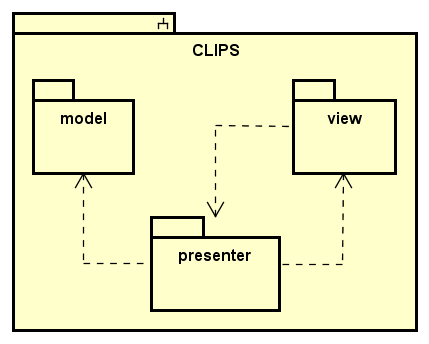
\includegraphics[scale=0.8]{img/package/CLIPS}
			\label{CLIPS}
			\caption{Diagramma dei package - sistema CLIPS}
		\end{figure}
		
	
	% componenti da esportare da Tracy
	\subsection{Componenti}

\subsubsection{model}

    \begin{figure}[H]
        \centering
        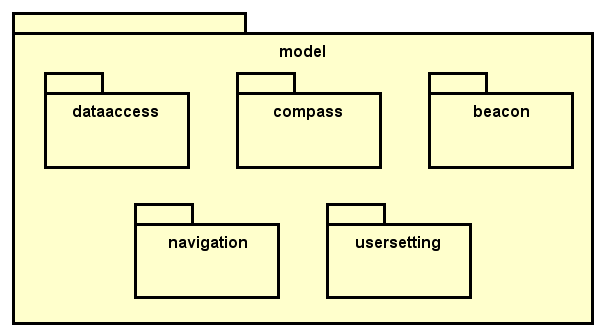
\includegraphics{img/package/model.png}
        \caption{Componente model}\label{fig:model} 
    \end{figure}
    \begin{itemize}
\item \textbf{Descrizione:} Package per il componente Model del pattern architetturale MVP. Questo pacchetto contiene tutte le classi che compongono la business logic;
\item \textbf{Package Contenuti}:
\begin{itemize}
\item \texttt{beacon};

\item \texttt{compass};

\item \texttt{dataaccess};

\item \texttt{navigator};

\item \texttt{usersetting}.

\end{itemize}
\item \textbf{Classi Contenute}:
\begin{itemize}
\item \texttt{AbsBeaconReceiverManager};

\item \texttt{InformationManagerImp};

\item \texttt{MessageSendType};

\item \texttt{NavigationManagerImp};

\item \texttt{NoBeaconSeenException};

\item \texttt{ServiceConnectionImp}.

\end{itemize}
\item \textbf{Interfacce Contenute}:
\begin{itemize}
\item \texttt{InformationManager};

\item \texttt{NavigationManager}.

\end{itemize}
\end{itemize}

\subsubsection{model::\-beacon}

    \begin{figure}[H]
        \centering
        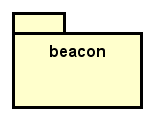
\includegraphics{img/package/beacon.png}
        \caption{Componente model::\-beacon}\label{fig:model::beacon} 
    \end{figure}
    \begin{itemize}
\item \textbf{Descrizione:} Package contenente le classi che rappresentano o si occupano della rilevazione dei beacon. Questo package ha inoltre il compito di interfacciarsi con la libreria Altbeacon;
\item \textbf{Padre:} \texttt{model};
\item \textbf{Classi Contenute}:
\begin{itemize}
\item \texttt{BeaconManagerAdapter};

\item \texttt{LocalBinder};

\item \texttt{LoggerImp};

\item \texttt{MyBeaconImp};

\item \texttt{MyDistanceCalculator}.

\end{itemize}
\item \textbf{Interfacce Contenute}:
\begin{itemize}
\item \texttt{BeaconRanger};

\item \texttt{Logger};

\item \texttt{MyBeacon}.

\end{itemize}
\end{itemize}

\subsubsection{model::\-compass}

    \begin{figure}[H]
        \centering
        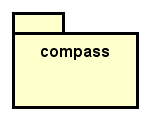
\includegraphics{img/package/compass.png}
        \caption{Componente model::\-compass}\label{fig:model::compass} 
    \end{figure}
    \begin{itemize}
\item \textbf{Descrizione:} Package per la gestione della bussola;
\item \textbf{Padre:} \texttt{model};
\item \textbf{Classi Contenute}:
\begin{itemize}
\item \texttt{Compass}.

\end{itemize}
\end{itemize}

\subsubsection{model::\-dataaccess}

    \begin{figure}[H]
        \centering
        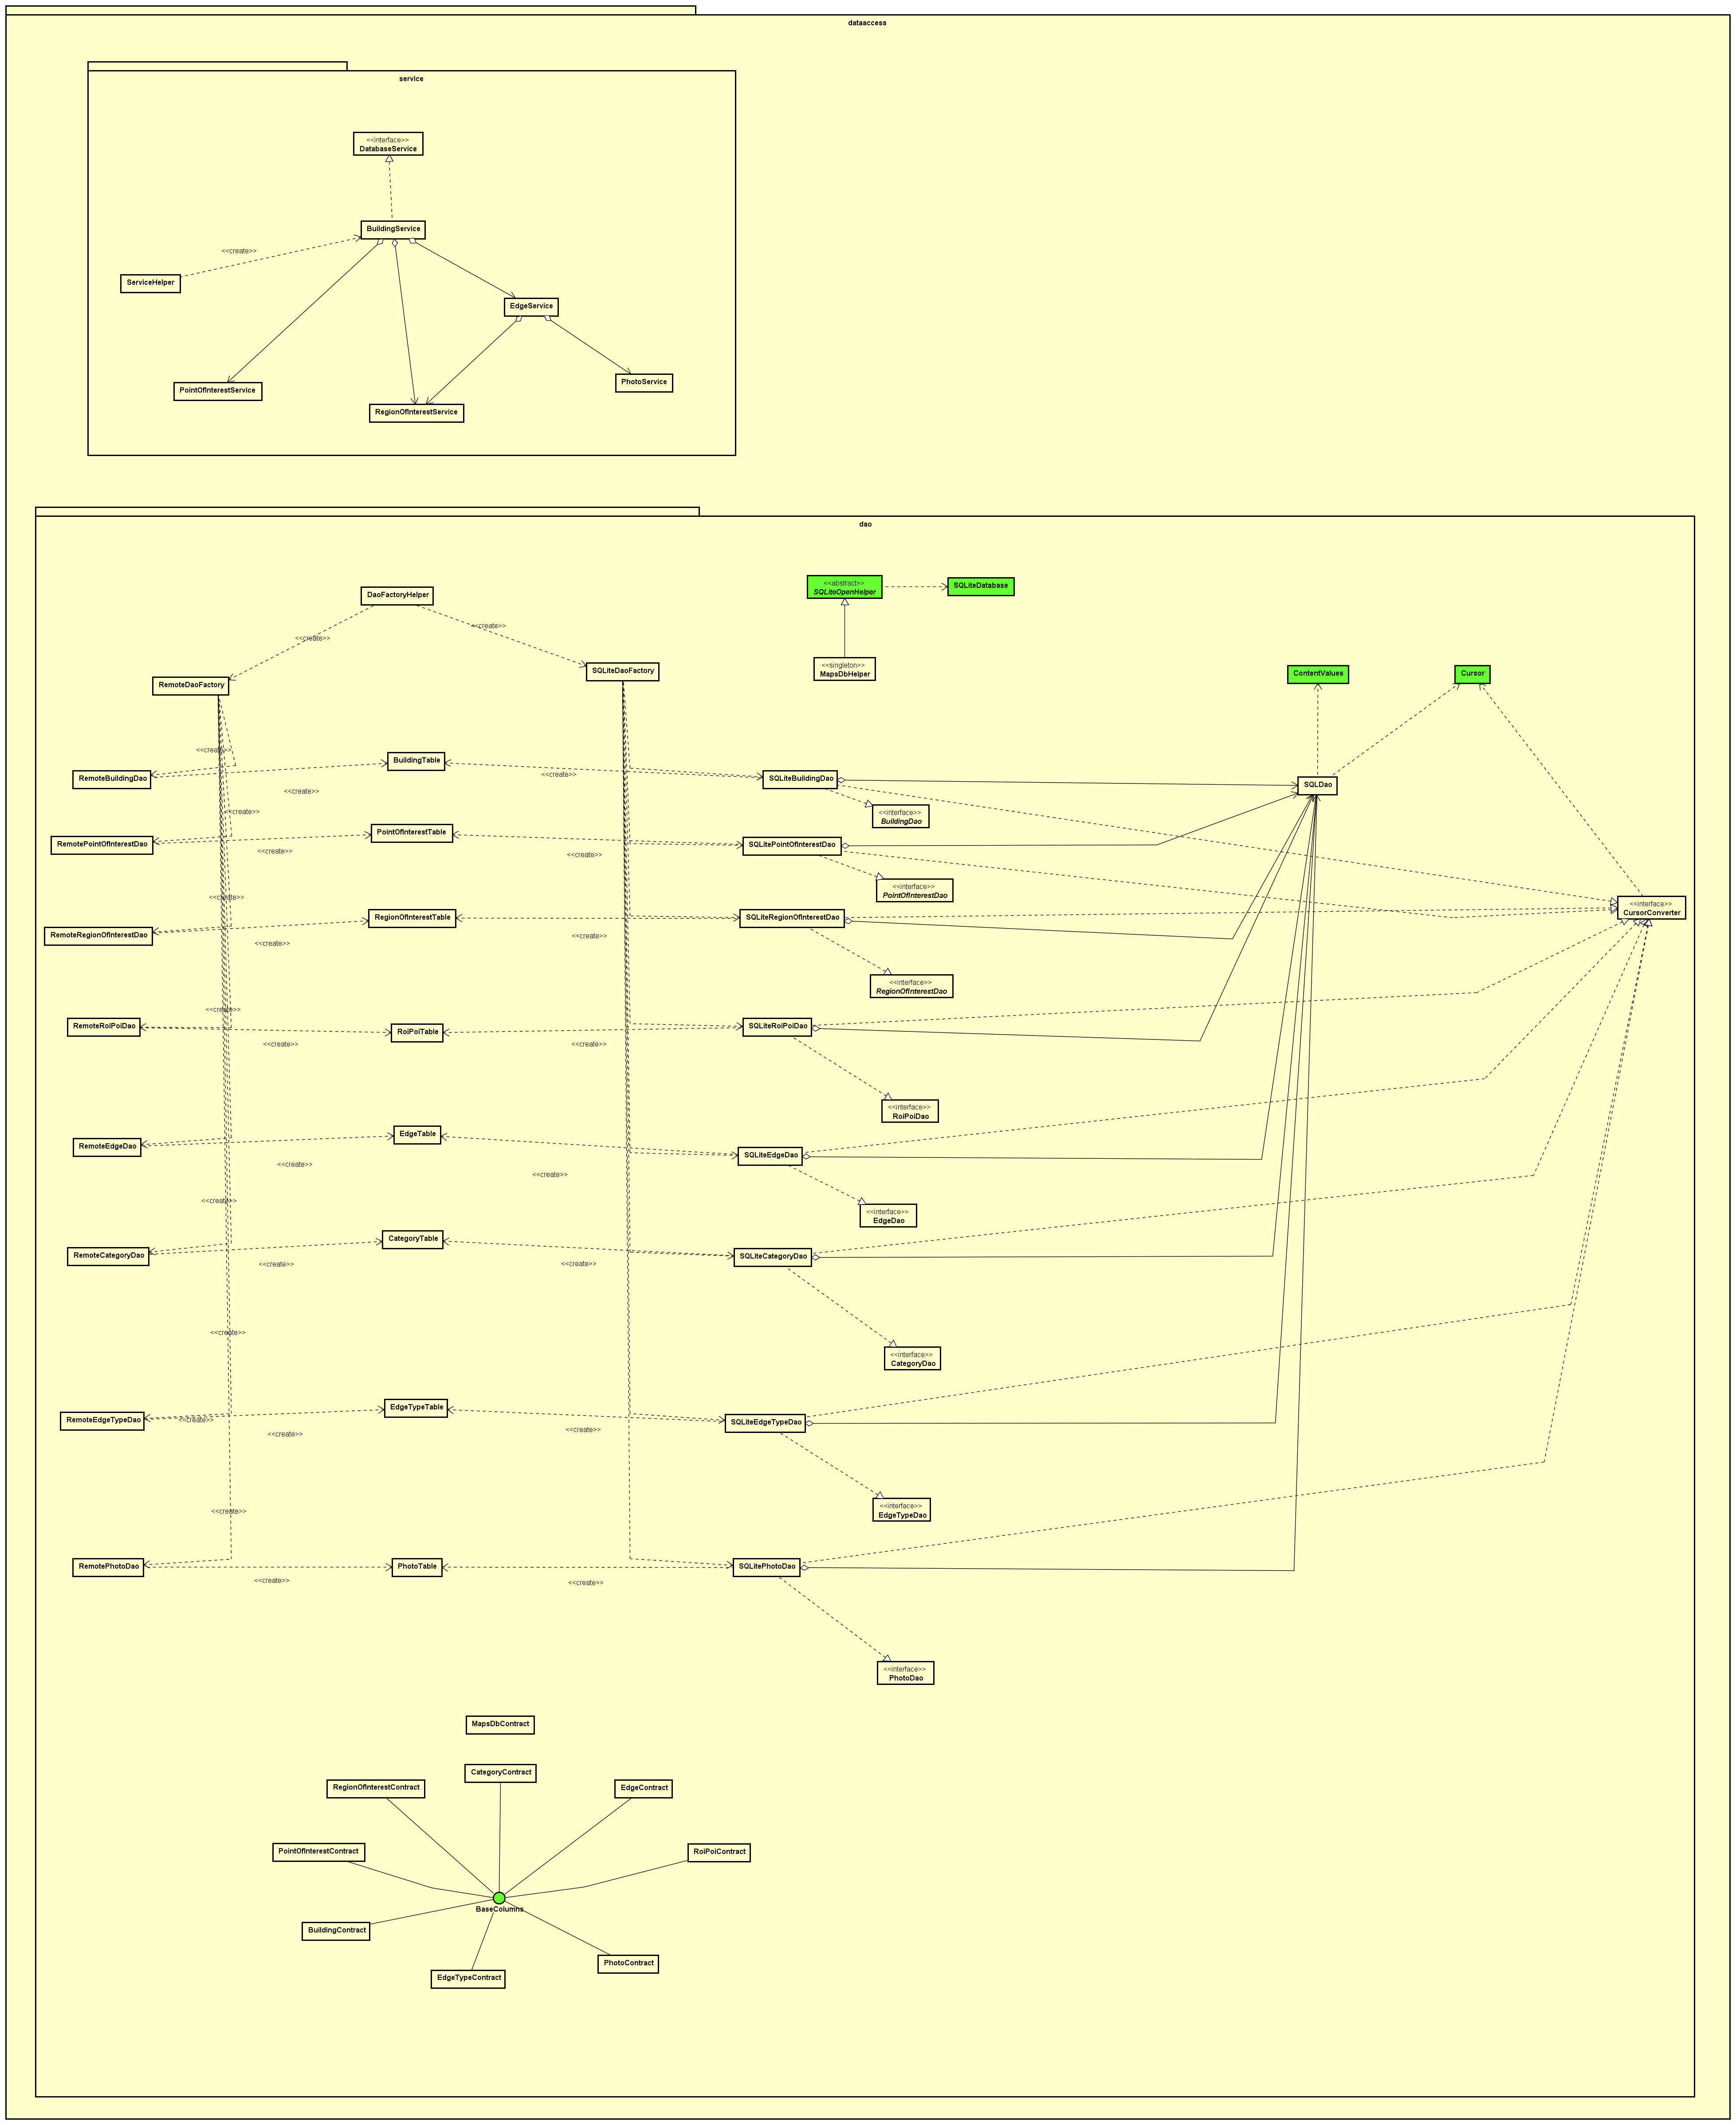
\includegraphics{img/package/dataaccess.png}
        \caption{Componente model::\-dataaccess}\label{fig:model::dataaccess} 
    \end{figure}
    \begin{itemize}
\item \textbf{Descrizione:} Package per la gestione dell'accesso ai dati del database locale e remoto;
\item \textbf{Padre:} \texttt{model};
\item \textbf{Package Contenuti}:
\begin{itemize}
\item \texttt{dao};

\item \texttt{service}.

\end{itemize}
\end{itemize}

\subsubsection{model::\-dataaccess::\-dao}

    \begin{figure}[H]
        \centering
        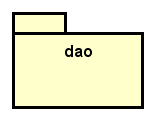
\includegraphics{img/package/dao.png}
        \caption{Componente model::\-dataaccess::\-dao}\label{fig:model::dataaccess::dao} 
    \end{figure}
    \begin{itemize}
\item \textbf{Descrizione:} Package che permette l'interazione diretta con il database e di costruire oggetti persistenti a partire dai risultati delle query sul database;
\item \textbf{Padre:} \texttt{dataaccess};
\item \textbf{Classi Contenute}:
\begin{itemize}
\item \texttt{BuildingContract};

\item \texttt{BuildingTable};

\item \texttt{CategoryContract};

\item \texttt{CategoryTable};

\item \texttt{DaoFactoryHelper};

\item \texttt{EdgeContract};

\item \texttt{EdgeTable};

\item \texttt{EdgeTypeContract};

\item \texttt{EdgeTypeTable};

\item \texttt{MapsDbContract};

\item \texttt{MapsDbHelper};

\item \texttt{PhotoContract};

\item \texttt{PhotoTable};

\item \texttt{PointOfInterestContract};

\item \texttt{PointOfInterestTable};

\item \texttt{RegionOfInterestContract};

\item \texttt{RegionOfInterestTable};

\item \texttt{RemoteBuildingDao};

\item \texttt{RemoteCategoryDao};

\item \texttt{RemoteDaoFactory};

\item \texttt{RemoteEdgeDao};

\item \texttt{RemoteEdgeTypeDao};

\item \texttt{RemotePhotoDao};

\item \texttt{RemotePointOfInterestDao};

\item \texttt{RemoteRegionOfInterestDao};

\item \texttt{RemoteRoiPoiDao};

\item \texttt{RoiPoiContract};

\item \texttt{RoiPoiTable};

\item \texttt{SQLDao};

\item \texttt{SQLiteBuildingDao};

\item \texttt{SQLiteCategoryDao};

\item \texttt{SQLiteDaoFactory};

\item \texttt{SQLiteEdgeDao};

\item \texttt{SQLiteEdgeTypeDao};

\item \texttt{SQLitePhotoDao};

\item \texttt{SQLitePointOfInterestDao};

\item \texttt{SQLiteRegionOfInterestDao};

\item \texttt{SQLiteRoiPoiDao}.

\end{itemize}
\item \textbf{Interfacce Contenute}:
\begin{itemize}
\item \texttt{BuildingDao};

\item \texttt{CategoryDao};

\item \texttt{CursorConverter};

\item \texttt{EdgeDao};

\item \texttt{EdgeTypeDao};

\item \texttt{PhotoDao};

\item \texttt{PointOfInterestDao};

\item \texttt{RegionOfInterestDao};

\item \texttt{RoiPoiDao}.

\end{itemize}
\end{itemize}

\subsubsection{model::\-dataaccess::\-service}

    \begin{figure}[H]
        \centering
        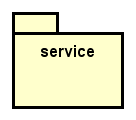
\includegraphics{img/package/service.png}
        \caption{Componente model::\-dataaccess::\-service}\label{fig:model::dataaccess::service} 
    \end{figure}
    \begin{itemize}
\item \textbf{Descrizione:} Package per la creazione degli oggetti della business logic a partire da oggetti DAO;
\item \textbf{Padre:} \texttt{dataaccess};
\item \textbf{Classi Contenute}:
\begin{itemize}
\item \texttt{BuildingService};

\item \texttt{EdgeService};

\item \texttt{PhotoService};

\item \texttt{PointOfInterestService};

\item \texttt{RegionOfInterestService};

\item \texttt{ServiceHelper}.

\end{itemize}
\item \textbf{Interfacce Contenute}:
\begin{itemize}
\item \texttt{DatabaseService}.

\end{itemize}
\end{itemize}

\subsubsection{model::\-navigator}

    \begin{figure}[H]
        \centering
        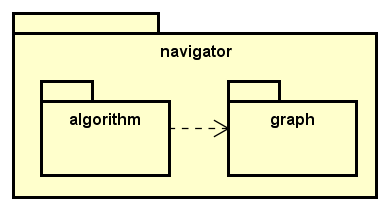
\includegraphics{img/package/navigator.png}
        \caption{Componente model::\-navigator}\label{fig:model::navigator} 
    \end{figure}
    \begin{itemize}
\item \textbf{Descrizione:} Package contenente le classi che permettono la navigazione all'interno degli edifici per cui è previsto il servizio e di accedere alle informazioni relative a tali edifici;
\item \textbf{Padre:} \texttt{model};
\item \textbf{Package Contenuti}:
\begin{itemize}
\item \texttt{algorithm};

\item \texttt{graph}.

\end{itemize}
\item \textbf{Classi Contenute}:
\begin{itemize}
\item \texttt{BuildingInformation};

\item \texttt{BuildingMapImp};

\item \texttt{NavigationExceptions};

\item \texttt{NavigatorImp};

\item \texttt{NoGraphSetException};

\item \texttt{NoNavigationInformationException};

\item \texttt{PathException};

\item \texttt{ProcessedInformationImp}.

\end{itemize}
\item \textbf{Interfacce Contenute}:
\begin{itemize}
\item \texttt{BuildingMap};

\item \texttt{Navigator};

\item \texttt{ProcessedInformation}.

\end{itemize}
\end{itemize}

\subsubsection{model::\-navigator::\-algorithm}

    \begin{figure}[H]
        \centering
        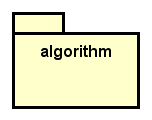
\includegraphics{img/package/algorithm.png}
        \caption{Componente model::\-navigator::\-algorithm}\label{fig:model::navigator::algorithm} 
    \end{figure}
    \begin{itemize}
\item \textbf{Descrizione:} Package contenente le classi che si occupano del calcolo dei percorsi da seguire per la navigazione;
\item \textbf{Padre:} \texttt{navigator};
\item \textbf{Classi Contenute}:
\begin{itemize}
\item \texttt{DijkstraPathFinder}.

\end{itemize}
\item \textbf{Interfacce Contenute}:
\begin{itemize}
\item \texttt{PathFinder}.

\end{itemize}
\end{itemize}

\subsubsection{model::\-navigator::\-graph}

    \begin{figure}[H]
        \centering
        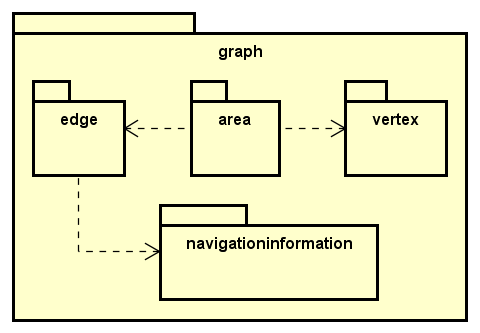
\includegraphics{img/package/graph.png}
        \caption{Componente model::\-navigator::\-graph}\label{fig:model::navigator::graph} 
    \end{figure}
    \begin{itemize}
\item \textbf{Descrizione:} Package contenente le classi che permettono la rappresentazione di un edificio sottoforma di grafo;
\item \textbf{Padre:} \texttt{navigator};
\item \textbf{Package Contenuti}:
\begin{itemize}
\item \texttt{area};

\item \texttt{edge};

\item \texttt{navigationinformation};

\item \texttt{vertex}.

\end{itemize}
\item \textbf{Classi Contenute}:
\begin{itemize}
\item \texttt{MapGraph}.

\end{itemize}
\end{itemize}

\subsubsection{model::\-navigator::\-graph::\-area}

    \begin{figure}[H]
        \centering
        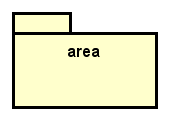
\includegraphics{img/package/area.png}
        \caption{Componente model::\-navigator::\-graph::\-area}\label{fig:model::navigator::graph::area} 
    \end{figure}
    \begin{itemize}
\item \textbf{Descrizione:} Package contenente le classi per rappresentare le aree interne di un edificio;
\item \textbf{Padre:} \texttt{graph};
\item \textbf{Interazione con componenti}:
\begin{itemize}
\item \texttt{model::navigator::graph::vertex}
\end{itemize}
\item \textbf{Classi Contenute}:
\begin{itemize}
\item \texttt{PointOfInterestImp};

\item \texttt{PointOfInterestInformation};

\item \texttt{RegionOfInterestImp}.

\end{itemize}
\item \textbf{Interfacce Contenute}:
\begin{itemize}
\item \texttt{PointOfInterest};

\item \texttt{RegionOfInterest}.

\end{itemize}
\end{itemize}

\subsubsection{model::\-navigator::\-graph::\-edge}

    \begin{figure}[H]
        \centering
        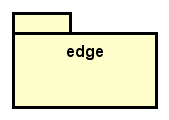
\includegraphics{img/package/edge.png}
        \caption{Componente model::\-navigator::\-graph::\-edge}\label{fig:model::navigator::graph::edge} 
    \end{figure}
    \begin{itemize}
\item \textbf{Descrizione:} Package contenenti le classi per la rappresentazione di un arco di un grafo. Questo package contiene inoltre le classi per rappresentare degli archi che contengono informazione;
\item \textbf{Padre:} \texttt{graph};
\item \textbf{Classi Contenute}:
\begin{itemize}
\item \texttt{AbsEnrichedEdge};

\item \texttt{DefaultEdge};

\item \texttt{ElevatorEdge};

\item \texttt{StairEdge}.

\end{itemize}
\item \textbf{Interfacce Contenute}:
\begin{itemize}
\item \texttt{Edge};

\item \texttt{EnrichedEdge}.

\end{itemize}
\end{itemize}

\subsubsection{model::\-navigator::\-graph::\-navigationinformation}

    \begin{figure}[H]
        \centering
        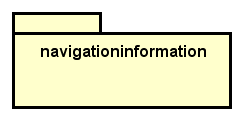
\includegraphics{img/package/navigationinformation.png}
        \caption{Componente model::\-navigator::\-graph::\-navigationinformation}\label{fig:model::navigator::graph::navigationinformation} 
    \end{figure}
    \begin{itemize}
\item \textbf{Descrizione:} Package contenente le classi per la rappresentazione delle informazioni di navigazione;
\item \textbf{Padre:} \texttt{graph};
\item \textbf{Classi Contenute}:
\begin{itemize}
\item \texttt{BasicInformation};

\item \texttt{DetailedInformation};

\item \texttt{NavigationInformationImp};

\item \texttt{PhotoInformation};

\item \texttt{PhotoRef}.

\end{itemize}
\item \textbf{Interfacce Contenute}:
\begin{itemize}
\item \texttt{NavigationInformation}.

\end{itemize}
\end{itemize}

\subsubsection{model::\-navigator::\-graph::\-vertex}

    \begin{figure}[H]
        \centering
        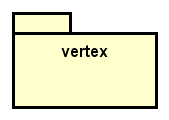
\includegraphics{img/package/vertex.png}
        \caption{Componente model::\-navigator::\-graph::\-vertex}\label{fig:model::navigator::graph::vertex} 
    \end{figure}
    \begin{itemize}
\item \textbf{Descrizione:} Package contenente le classi per la rappresentazione di un vertice del grafo;
\item \textbf{Padre:} \texttt{graph};
\item \textbf{Interazione con componenti}:
\begin{itemize}
\item \texttt{model::navigator::graph::area}
\end{itemize}
\item \textbf{Classi Contenute}:
\begin{itemize}
\item \texttt{VertexImp}.

\end{itemize}
\item \textbf{Interfacce Contenute}:
\begin{itemize}
\item \texttt{Vertex}.

\end{itemize}
\end{itemize}

\subsubsection{model::\-usersetting}

    \begin{figure}[H]
        \centering
        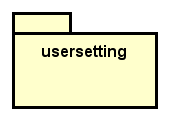
\includegraphics{img/package/usersetting.png}
        \caption{Componente model::\-usersetting}\label{fig:model::usersetting} 
    \end{figure}
    \begin{itemize}
\item \textbf{Descrizione:} Package contenente le classi che si occupano della gestione delle impostazioni e delle preferenze dell'utente. In particolare si occupano della gestione delle preferenze di navigazione e di fruizione delle informazioni e, inoltre, della gestione dei codici sviluppatore;
\item \textbf{Padre:} \texttt{model};
\item \textbf{Classi Contenute}:
\begin{itemize}
\item \texttt{DeveloperCodeManager};

\item \texttt{InstructionPreference};

\item \texttt{PathPreference};

\item \texttt{SettingImp}.

\end{itemize}
\item \textbf{Interfacce Contenute}:
\begin{itemize}
\item \texttt{Setting}.

\end{itemize}
\end{itemize}

\subsubsection{presenter}

    \begin{figure}[H]
        \centering
        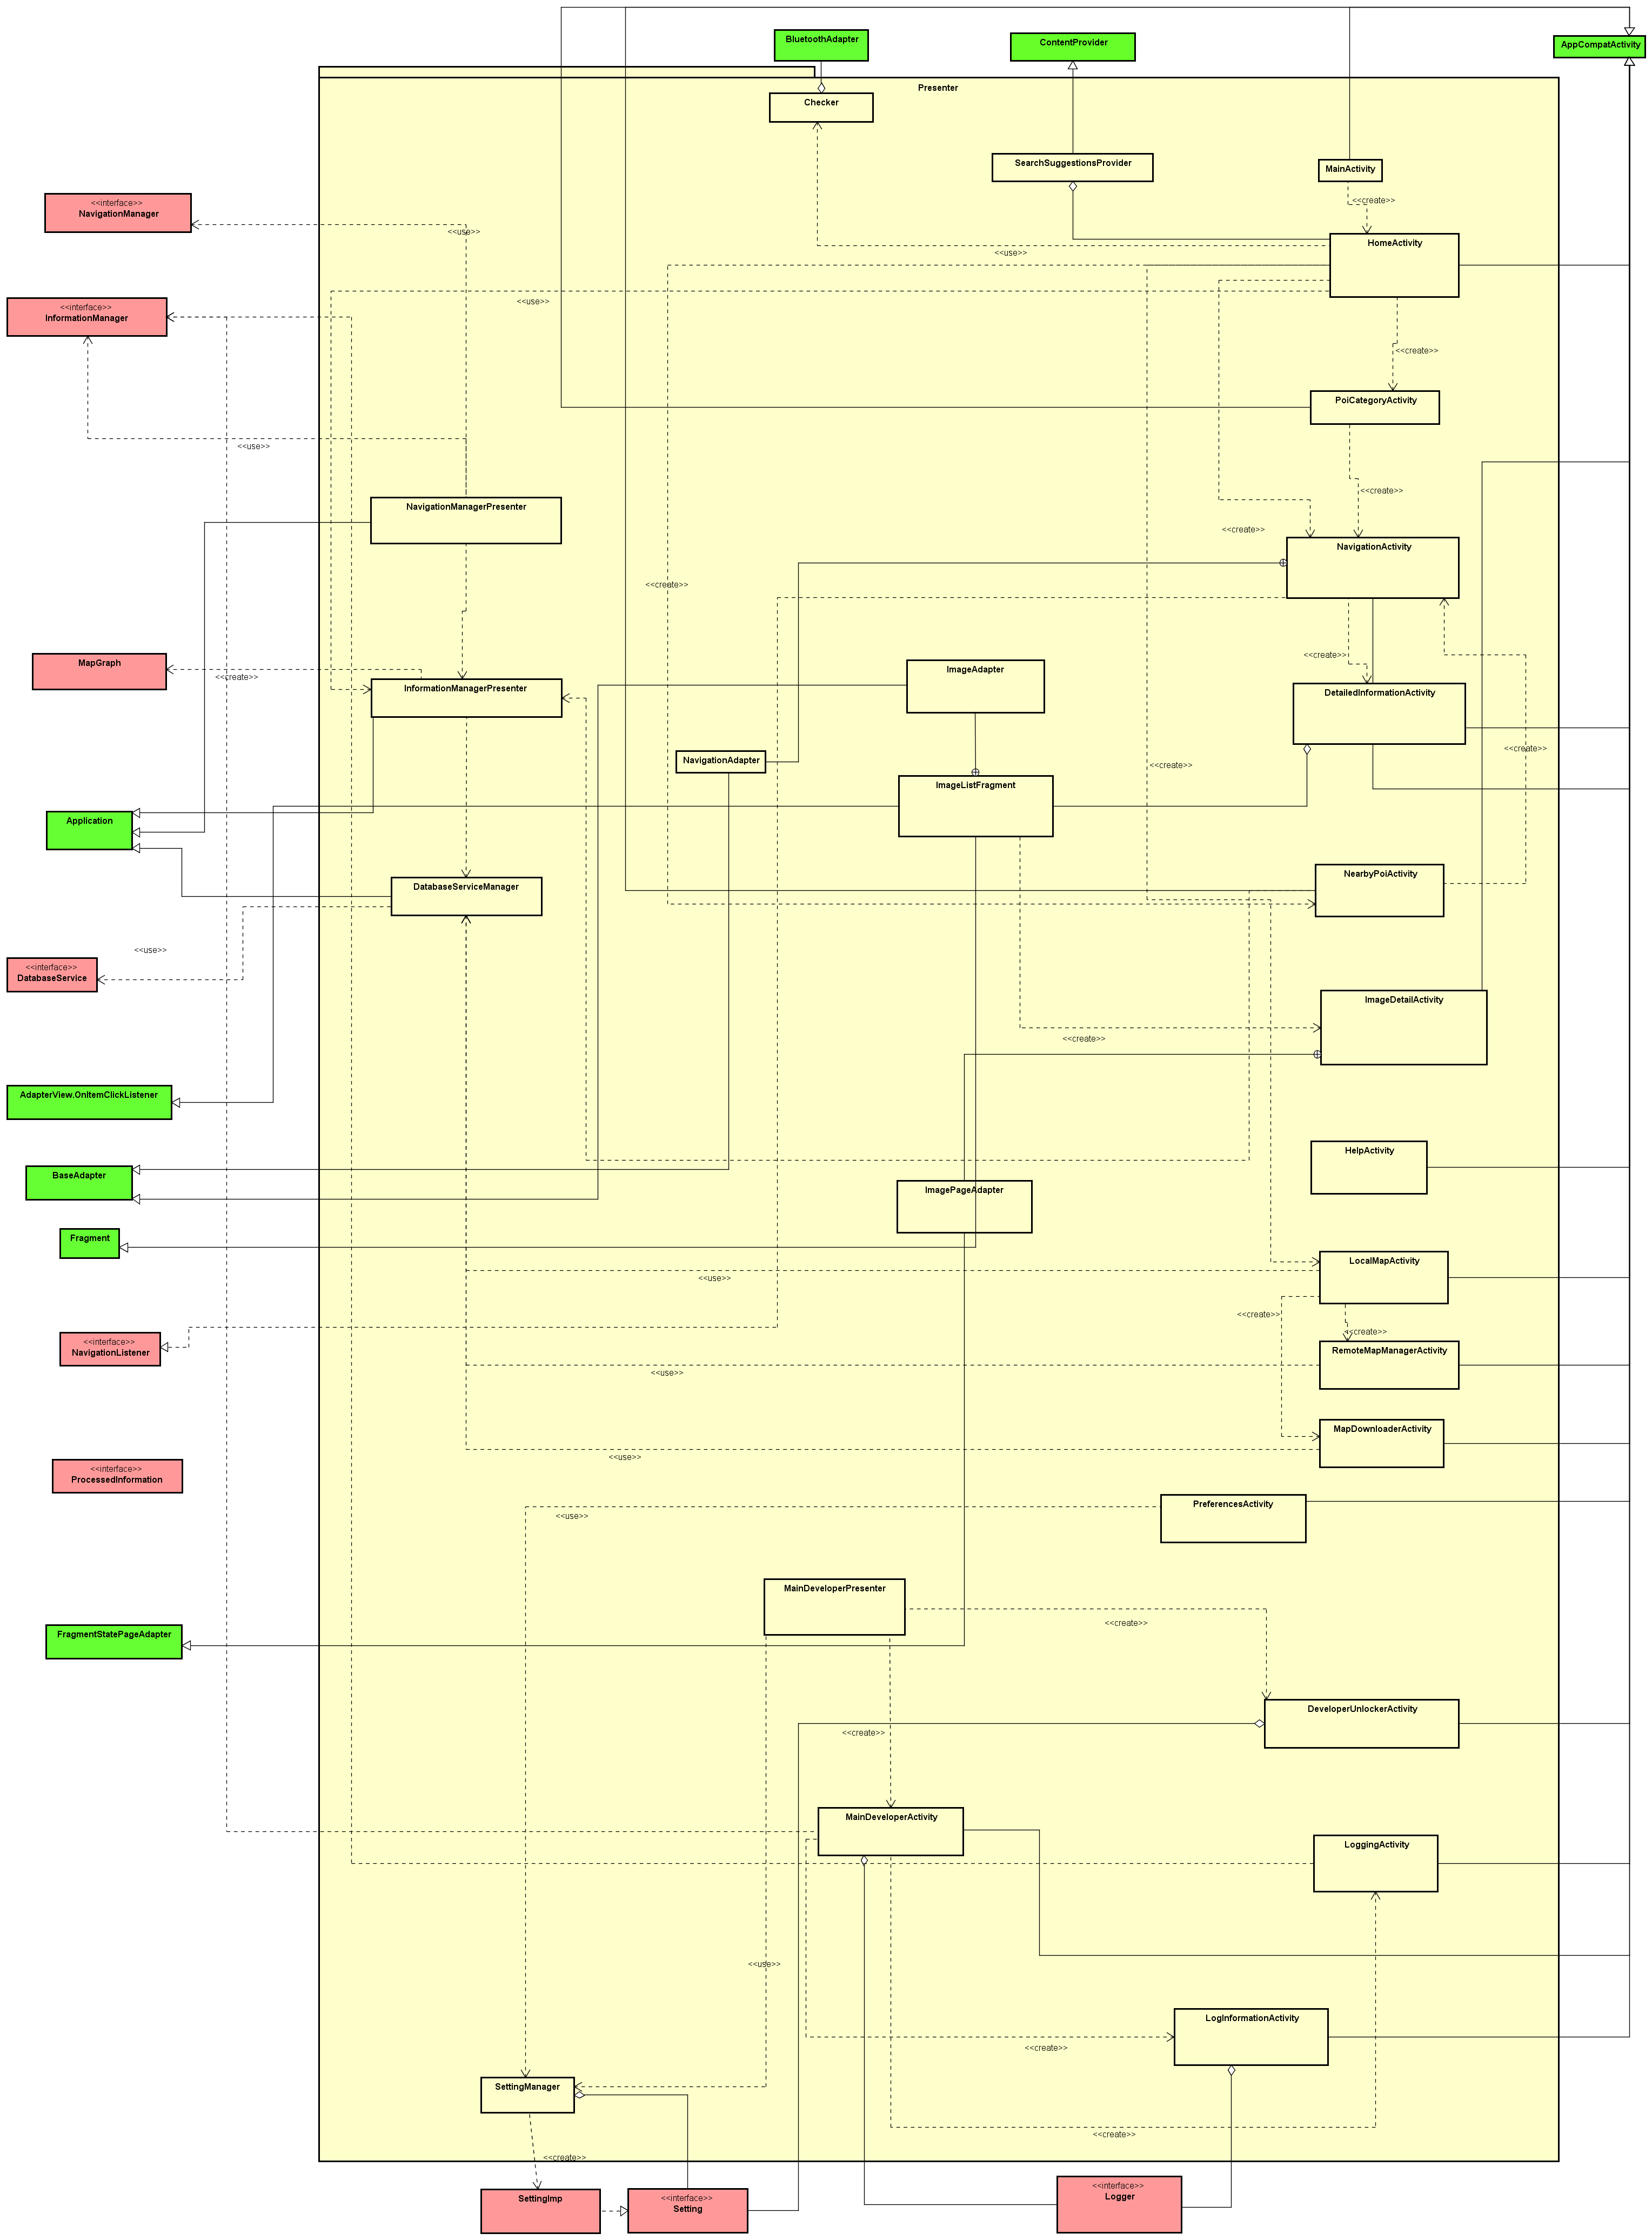
\includegraphics{img/package/presenter.png}
        \caption{Componente presenter}\label{fig:presenter} 
    \end{figure}
    \begin{itemize}
\item \textbf{Descrizione:} Package per il componente Presenter del pattern architetturale MVP;
\item \textbf{Classi Contenute}:
\begin{itemize}
\item \texttt{Checker};

\item \texttt{DatabaseServiceManager};

\item \texttt{DetailedInformationActivity};

\item \texttt{DeveloperUnlockerActivity};

\item \texttt{HelpActivity};

\item \texttt{HomeActivity};

\item \texttt{ImageAdapter};

\item \texttt{ImageDetailActivity};

\item \texttt{ImageListFragment};

\item \texttt{ImagePageAdapter};

\item \texttt{InformationManagerPresenter};

\item \texttt{LocalMapActivity};

\item \texttt{LoggingActivity};

\item \texttt{LogInformationActivity};

\item \texttt{MainActivity};

\item \texttt{MainDeveloperActivity};

\item \texttt{MainDeveloperPresenter};

\item \texttt{MapDownloaderActivity};

\item \texttt{NavigationActivity};

\item \texttt{NavigationAdapter};

\item \texttt{NavigationManagerPresenter};

\item \texttt{NearbyPoiActivity};

\item \texttt{PoiCategoryActivity};

\item \texttt{PreferencesActivity};

\item \texttt{RemoteMapManagerActivity};

\item \texttt{SearchSuggestionsProvider};

\item \texttt{SettingManager}.

\end{itemize}
\end{itemize}

\subsubsection{view}

    \begin{figure}[H]
        \centering
        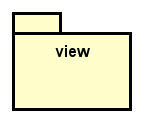
\includegraphics{img/package/view.png}
        \caption{Componente view}\label{fig:view} 
    \end{figure}
    \begin{itemize}
\item \textbf{Descrizione:} Package per il componente View del pattern architetturale MVP. Questo pacchetto contiene tutte le classi che compongono la presentation logic;
\item \textbf{Classi Contenute}:
\begin{itemize}
\item \texttt{DetailedInformationViewImp};

\item \texttt{DeveloperUnlockerViewImp};

\item \texttt{HelpViewImp};

\item \texttt{HomeViewImp};

\item \texttt{ImageDetailViewImp};

\item \texttt{ImageListFragmentViewImp};

\item \texttt{LocalMapManagerViewImp};

\item \texttt{LoggingViewImp};

\item \texttt{LogInformationViewImp};

\item \texttt{MainDeveloperViewImp};

\item \texttt{MainViewImp};

\item \texttt{MapDownloaderViewImp};

\item \texttt{NavigationViewImp};

\item \texttt{NearbyPoiViewImp};

\item \texttt{PoiCategoryViewImp};

\item \texttt{PreferencesViewImp};

\item \texttt{RemoteMapManagerViewImp}.

\end{itemize}
\item \textbf{Interfacce Contenute}:
\begin{itemize}
\item \texttt{DetailedInformationView};

\item \texttt{DeveloperUnlockerView};

\item \texttt{HelpView};

\item \texttt{HomeView};

\item \texttt{ImageDetailView};

\item \texttt{ImageListFragmentView};

\item \texttt{LocalMapManagerView};

\item \texttt{LoggingView};

\item \texttt{LogInformationView};

\item \texttt{MainDeveloperView};

\item \texttt{MainView};

\item \texttt{MapDownloaderView};

\item \texttt{NavigationView};

\item \texttt{NearbyPoiView};

\item \texttt{PoiCategoryView};

\item \texttt{PreferencesView};

\item \texttt{RemoteMapManagerView}.

\end{itemize}
\end{itemize}
\subsection{Classi}

\subsubsection{model::AbsBeaconReceiverManager}

    \begin{figure}[H]
        \centering
        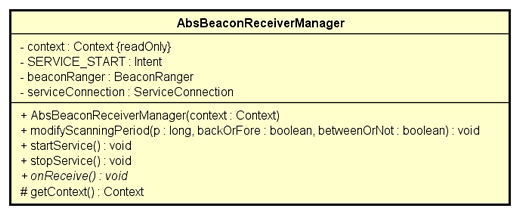
\includegraphics{img/AbsBeaconReceiverManager.png}
        \caption{Classe astratta AbsBeaconReceiverManager}\label{fig:model::AbsBeaconReceiverManager} 
    \end{figure}
    \begin{description}
\item[Nome:] \texttt{\textit{AbsBeaconReceiverManager}};
\item[Tipo:] Classe astratta;
\item[Estende:] \
\begin{itemize}
\item \texttt{ServiceConnectionImp}.
\end{itemize}
\item[Componenti delle librerie utilizzate:] \
\begin{itemize}
\item \texttt{android.content.BroadcastReceiver (Android)};

\item \texttt{android.content.Context (Android)};

\item \texttt{android.content.IntentFilter (Android)}.

\end{itemize}
\item[Visibilità:] \texttt{public};
\item[Utilizzo:] È utilizzata per implementare metodi utili a tutte le classi che necessitano di ricevere e utilizzare beacon;
\item[Descrizione:] Classe base per la comunicazione con le classi che si occupano del rilevamento dei beacon;
\item[Attributi:] \
\begin{itemize}
\item \texttt{- beaconManagerAdapter : BeaconRanger \{readOnly\}}\\
Service che si occupa del rilevamento dei beacon

\item \texttt{- context : Context \{readOnly\}}\\
Contesto dell'applicazione

\item \texttt{- serviceConnection : ServiceConnection}\\
Connessione con il Service per la comunicazione con il service stesso

\item \texttt{- \underline{SERVICE\_START : Intent \{readOnly\}}}\\
Intent per ricevere I beacon inviati dal BeaconManagerAdapter

\end{itemize}
\item[Metodi:] \
\begin{itemize}
\item \texttt{+ AbsBeaconReceiverManager()}\\
Costruttore della classe AbsBeaconReceiverManager
 \item \texttt{\# getContext() : Context}\\
Metodo che ritorna il contesto dell'applicazione
 \item \texttt{+ modifyScanningPeriod(p : long, backOrFore : boolean, betweenOrNot : boolean) : void}\\
Metodo che permette di modificare il tempo tra una scansione per la ricerca dei beaccon e la successiva
 \begin{description}
\item[Argomenti:] \
\begin{itemize}
\item \texttt{p : long}\\
Periodo di scansione dei beacon da scansionare\item \texttt{backOrFore : boolean}\\
Scelta se modificare il periodo di scansione quando l'applicazione è in background o in foreground\item \texttt{betweenOrNot : boolean}\\
Scelta se modificare il periodo di scansione o la pausa tra due scansioni\end{itemize}
\end{description}
\item \texttt{+ \textit{onReceive() : void}}\\
Metodo astratto che permette di eseguire delle azioni alla ricezione di una PriorityQueue<MyBeacon> contenente l'insieme dei beacon visibili in un determinato momento
 \item \texttt{+ startService() : void}\\
Metodo che permette di attivare il service che si occupa di fare le scansioni per trovare I beacon
 \item \texttt{+ stopService() : void}\\
Metodo che permette di fermare il service che si occupa di fare le scansioni per trovare I beacon
 \end{itemize}
\end{description}

\subsubsection{model::InformationManager}

    \begin{figure}[H]
        \centering
        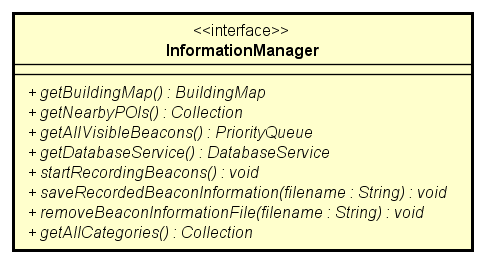
\includegraphics{img/InformationManager.png}
        \caption{Interfaccia InformationManager}\label{fig:model::InformationManager} 
    \end{figure}
    \begin{description}
\item[Nome:] \texttt{\textit{InformationManager}};
\item[Tipo:] Interfaccia;
\item[Visibilità:] \texttt{public};
\item[Utilizzo:] È utilizzata per rendere indipendente l'accesso alle informazioni trattate dai pacchetti del Model da come questo è realizzato;
\item[Descrizione:] Interfaccia che si occupa di esporre tutti i metodi utili per accedere ad informazioni trattate dai vari pacchetti del Model;
\item[Metodi:] \
\begin{itemize}
\item \texttt{+ \textit{getAllCategories() : Collection<String>}}\\
Metodo che ritorna tutte le categorie di POI all'interno dell'edificio
 \item \texttt{+ \textit{getAllVisibleBeacons() : PriorityQueue<MyBeacon>}}\\
Metodo che ritorna la PriorityQueue<MyBeacon>, eventualmente vuota, dei beacon visibili
 \item \texttt{+ \textit{getBuildingMap() : BuildingMap}}\\
Metodo che ritorna la mappa dell'edificio se questa è già stata caricata dal database locale. Viene lanciata una eccezione di tipo NoBeaconSeenException nel caso in cui non sia stata caricata la mappa poichè non è stato ancora ricevuto alcun beacon
 \item \texttt{+ \textit{getDatabaseService() : DatabaseService}}\\
Metodo che ritorna un oggetto DatabaseService che permette di interrogare il database
 \item \texttt{+ \textit{getLogInfo(name : String) : String}}\\
Metodo che, dato il nome di un log, ritorna l'informazione in esso contenuta sotto forma di stringa
 \begin{description}
\item[Argomenti:] \
\begin{itemize}
\item \texttt{name : String}\\
Nome del file di log da cui reperire l'informazione\end{itemize}
\end{description}
\item \texttt{+ \textit{getNearbyPOIs() : Collection<PointOfInterest>}}\\
Metodo che ritorna l'insieme di POI associati al beacon rilevato con il segnale più potente. Viene lanciata una eccezione di tipo NoBeaconSeenException nel caso in cui venga invocato il metodo ma non è stato rilevato ancora alcun beacon
 \item \texttt{+ \textit{removeBeaconInformationFile(filename : String) : void}}\\
Metodo che permette di rimuovere un log delle informazioni dei beacon visibili
 \begin{description}
\item[Argomenti:] \
\begin{itemize}
\item \texttt{filename : String}\\
Nome del file da rimuovere\end{itemize}
\end{description}
\item \texttt{+ \textit{saveRecordedBeaconInformation(filename : String) : void}}\\
Metodo che permette di salvare il log delle informazioni dei beacon visibili su file
 \begin{description}
\item[Argomenti:] \
\begin{itemize}
\item \texttt{filename : String}\\
Nome da dare al file da salvare\end{itemize}
\end{description}
\item \texttt{+ \textit{startRecordingBeacons() : void}}\\
Metodo che permette di avviare il log delle informazioni dei beacon visibili
 \end{itemize}
\end{description}

\subsubsection{model::InformationManagerImp}

    \begin{figure}[H]
        \centering
        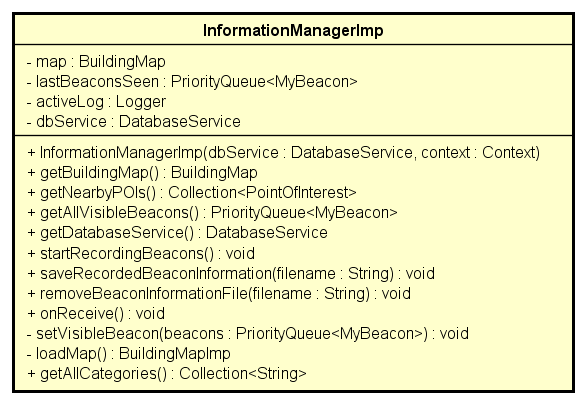
\includegraphics{img/InformationManagerImp.png}
        \caption{Classe InformationManagerImp}\label{fig:model::InformationManagerImp} 
    \end{figure}
    \begin{description}
\item[Nome:] \texttt{InformationManagerImp};
\item[Tipo:] Classe;
\item[Estende:] \
\begin{itemize}
\item \texttt{AbsBeaconReceiverManager}.
\end{itemize}
\item[Implementa:] \
\begin{itemize}
\item \texttt{InformationManager}.

\end{itemize}
\item[Visibilità:] \texttt{public};
\item[Utilizzo:] È utilizzata per avere un unico punto di accesso alle informazioni del package Model. La classe si occupa di tenere un riferimento alla mappa a cui appartengono i beacon rilevati, un riferimento all'interfaccia che permette di accedere alle informazioni salvate nel database locale o remoto e ti permette di salvare le informazioni dei beacon rilevati;
\item[Descrizione:] Classe che permette l'accesso alle informazioni trattate nel package Model;
\item[Attributi:] \
\begin{itemize}
\item \texttt{- activeLog : Logger}\\
Logger per la registrazione delle informazioni dei beacon rilevati

\item \texttt{- dbService : DatabaseService \{readOnly\}}\\
Oggetto per la gestione delle mappe nel database locale e per il recupero delle mappe nel database remoto

\item \texttt{- lastBeaconsSeen : PriorityQueue<MyBeacon>}\\
PriorityQueue, eventualmente vuota, contenente gli ultimi beacon rilevati

\item \texttt{- map : BuildingMap}\\
Mappa dell'edificio di cui sono stati rilevati I beacon

\end{itemize}
\item[Metodi:] \
\begin{itemize}
\item \texttt{+ getAllCategories() : Collection<String>}\\
Metodo che ritorna tutte le categorie di POI presenti all'interno dell'edificio
 \item \texttt{+ getAllVisibleBeacons() : PriorityQueue<MyBeacon>}\\
Metodo che ritorna la PriorityQueue<MyBeacon>, eventualmente vuota, dei beacon visibili
 \item \texttt{+ getBuildingMap() : BuildingMap}\\
Metodo che ritorna la mappa dell'edificio se questa è già stata caricata dal database locale. Viene lanciata una eccezione di tipo NoBeaconSeenException nel caso in cui non sia stata caricata la mappa poichè non è stato ancora ricevuto alcun beacon
 \item \texttt{+ getDatabaseService() : DatabaseService}\\
Metodo che ritorna un oggetto DatabaseService che permette di interrogare il database
 \item \texttt{+ getLogInfo(name : String) : String}\\
Metodo che, dato il nome di un log, ritorna l'informazione in esso contenuta sotto forma di stringa
 \begin{description}
\item[Argomenti:] \
\begin{itemize}
\item \texttt{name : String}\\
Nome del log da cui reperire l'informazione\end{itemize}
\end{description}
\item \texttt{+ getNearbyPOIs() : Collection<PointOfInterest>}\\
Metodo che ritorna l'insieme di POI associati al beacon rilevato con il segnale più potente. Viene lanciata una eccezione di tipo NoBeaconSeenException nel caso in cui venga invocato il metodo ma non è stato rilevato ancora alcun beacon
 \item \texttt{+ InformationManagerImp(dbService : DatabaseService, context : Context)}\\
Costruttore della classe InformationManagerImp
 \begin{description}
\item[Argomenti:] \
\begin{itemize}
\item \texttt{dbService : DatabaseService}\\
Oggetto per la gestione delle mappe nel database locale e per il recupero delle mappe nel database remoto\item \texttt{context : Context}\\
Contesto dell'applicazione\end{itemize}
\end{description}
\item \texttt{- loadMap() : BuildingMap}\\
Metodo che permette di recuperare una mappa dal database in base al major dei beacon rilevati
 \item \texttt{+ onReceive() : void}\\
Metodo che si occupa di settare il campo dati lastBeaconsSeen con la PriorityQueue<MyBeacon> contenente gli ultimi beacon rilevati. Nel caso in cui non sia stata ancora caricata una mappa dal database locale si occupa di caricare la mappa dell'edificio che contiene I beaccon rilevati
 \item \texttt{+ removeBeaconInformationFile(filename : String) : void}\\
Metodo che permette di rimuovere un log delle informazioni dei beacon visibili
 \begin{description}
\item[Argomenti:] \
\begin{itemize}
\item \texttt{filename : String}\\
Nome del file da rimuovere\end{itemize}
\end{description}
\item \texttt{+ saveRecordedBeaconInformation(filename : String) : void}\\
Metodo che permette di salvare il log delle informazioni dei beacon visibili su file
 \begin{description}
\item[Argomenti:] \
\begin{itemize}
\item \texttt{filename : String}\\
Nome del file in cui salvare le informazioni dei beacon\end{itemize}
\end{description}
\item \texttt{- setVisibleBeacon(beacons : PriorityQueue<MyBeacon>) : void}\\
Metodo che setta il campo dati lastBeaconsSeen
 \begin{description}
\item[Argomenti:] \
\begin{itemize}
\item \texttt{beacons : PriorityQueue<MyBeacon>}\\
Lista dei beacon visibili\end{itemize}
\end{description}
\item \texttt{+ startRecordingBeacons() : void}\\
Metodo che permette di avviare il log delle informazioni dei beacon visibili
 \end{itemize}
\end{description}

\subsubsection{model::MessageSendType}

    \begin{figure}[H]
        \centering
        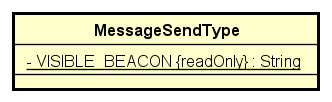
\includegraphics{img/MessageSendType.png}
        \caption{Classe MessageSendType}\label{fig:model::MessageSendType} 
    \end{figure}
    \begin{description}
\item[Nome:] \texttt{MessageSendType};
\item[Tipo:] Classe;
\item[Visibilità:] \texttt{public};
\item[Utilizzo:] È utilizzata dalla classe BeaconManagerAdapter per inviare messaggi contenenti la lista di beacon tramite una istanza della classe android.support.v4.content.LocalBroadcastManager, attraverso le classi android.content.IntentFilter e BeaconReceiver, per ricevere tali messaggi;
\item[Descrizione:] Classe che rappresenta l'etichetta di un messaggio scambiato all'interno dell'applicazione contenente una lista di beacon;
\item[Attributi:] \
\begin{itemize}
\item \texttt{- VISIBLE\_BEACON : String}\\
Rappresenta il messaggio che viene scambiato all'interno dell'applicazione

\end{itemize}
\end{description}

\subsubsection{model::NavigationManager}

    \begin{figure}[H]
        \centering
        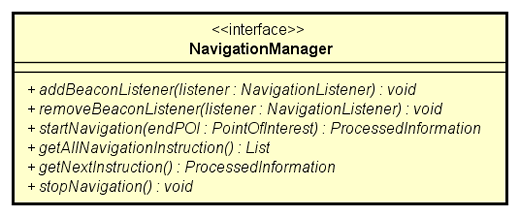
\includegraphics{img/NavigationManager.png}
        \caption{Interfaccia NavigationManager}\label{fig:model::NavigationManager} 
    \end{figure}
    \begin{description}
\item[Nome:] \texttt{\textit{NavigationManager}};
\item[Tipo:] Interfaccia;
\item[Visibilità:] \texttt{public};
\item[Utilizzo:] È utilizzata per rendere indipedente il modo in cui la navigazione è utilizzata da come questi metodi sono implementati;
\item[Descrizione:] Interfaccia che si occupa di esporre tutti i metodi utili alla navigazione;
\item[Metodi:] \
\begin{itemize}
\item \texttt{+ \textit{addBeaconListener(listener : NavigationListener) : void}}\\
Metodo che permette di registrare un listener
 \begin{description}
\item[Argomenti:] \
\begin{itemize}
\item \texttt{listener : NavigationListener}\\
Listener che deve essere aggiunto alla lista di NavigationListener\end{itemize}
\end{description}
\item \texttt{+ \textit{getAllNavigationInstruction() : List<ProcessedInformation>}}\\
Metodo che permette di recuperare tutte le istruzioni di navigazione per un percorso calcolato. Viene lanciata una eccezione di tipo NoNavigationInformationException nel caso in cui venga richiamato questo metodo senza aver prima avviato la navigazione
 \item \texttt{+ \textit{getNextInstruction() : ProcessedInformation}}\\
Metodo che permette di recuperare tutte le istruzioni di navigazione per un percorso calcolato in base al beacon più potente ricavato dalla PriorityQueue<MyBeacon> passata come argomento. Viene lanciata una eccezione di tipo NoNavigationInformationException nel caso in cui venga richiamato questo metodo senza aver prima avviato la navigazione.
 \item \texttt{+ \textit{removeBeaconListener(listener : NavigationListener) : void}}\\
Metodo che permette di rimuovere un listener
 \begin{description}
\item[Argomenti:] \
\begin{itemize}
\item \texttt{listener : NavigationListener}\\
Listener che deve essere rimosso dalla lista di NavigationListener\end{itemize}
\end{description}
\item \texttt{+ \textit{startCompass() : void}}\\
Metodo che permette di attivare il rilevamento dei dati dalla bussola
 \item \texttt{+ \textit{startNavigation(endPOI : PointOfInterest) : ProcessedInformation}}\\
Metodo che permette di avviare la navigazione verso uno specifico POI
 \begin{description}
\item[Argomenti:] \
\begin{itemize}
\item \texttt{endPOI : PointOfInterest}\\
POI da raggiungere tramite navigazione\end{itemize}
\end{description}
\item \texttt{+ \textit{stopCompass() : void}}\\
Metodo che permette di fermare il rilevamento dei dati ottenuti dalla bussola
 \item \texttt{+ \textit{stopNavigation() : void}}\\
Metodo che permette di fermare la navigazione
 \end{itemize}
\end{description}

\subsubsection{model::NavigationManagerImp}

    \begin{figure}[H]
        \centering
        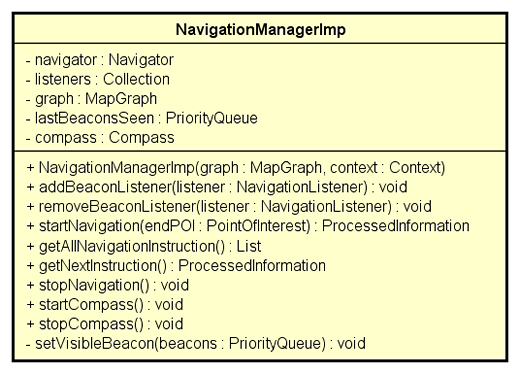
\includegraphics{img/NavigationManagerImp.png}
        \caption{Classe NavigationManagerImp}\label{fig:model::NavigationManagerImp} 
    \end{figure}
    \begin{description}
\item[Nome:] \texttt{NavigationManagerImp};
\item[Tipo:] Classe;
\item[Estende:] \
\begin{itemize}
\item \texttt{AbsBeaconReceiverManager}.
\end{itemize}
\item[Implementa:] \
\begin{itemize}
\item \texttt{NavigationManager}.

\end{itemize}
\item[Visibilità:] \texttt{public};
\item[Utilizzo:] È utilizzata per fornire istruzioni di navigazioni agli oggetti che osservano le istanza di tale classe, in base ai beacon rilevati;
\item[Descrizione:] Classe che si occupa della gestione della navigazione;
\item[Attributi:] \
\begin{itemize}
\item \texttt{- compass : Compass \{readOnly\}}\\
Oggetto che permette di recuperare I dati della bussola

\item \texttt{- graph : MapGraph \{readOnly\}}\\
Grafo rappresentante la mappa dell'edificio

\item \texttt{- lastBeaconsSeen : PriorityQueue<MyBeacon>}\\
PriorityQueue, eventualmente vuota, contenente gli ultimi beacon rilevati

\item \texttt{- listeners : Collection<NavigationListener>}\\
Collezione contenenti tutti I listener da aggiornare ad ogni nuova istruzione da inviare

\item \texttt{- navigator : Navigator}\\
Oggetto per la navigazione

\end{itemize}
\item[Metodi:] \
\begin{itemize}
\item \texttt{+ addBeaconListener(listener : NavigationListener) : void}\\
Metodo che permette di registrare un listener
 \begin{description}
\item[Argomenti:] \
\begin{itemize}
\item \texttt{listener : NavigationListener}\\
Listener che deve essere aggiunto alla lista di NavigationListener\end{itemize}
\end{description}
\item \texttt{+ getAllNavigationInstruction() : List<ProcessedInformation>}\\
Metodo che permette di recuperare tutte le istruzioni di navigazione per un percorso calcolato. Viene lanciata una eccezione di tipo NoNavigationInformationException nel caso in cui venga richiamato questo metodo senza aver prima avviato la navigazione
 \item \texttt{+ getNextInstruction() : ProcessedInformation}\\
Metodo che permette di recuperare tutte le istruzioni di navigazione per un percorso calcolato ion base al beacon più potente ricavato dalla PriorityQueue<MyBeacon> passata come argomento. Viene lanciata una eccezione di tipo NoNavigationInformationException nel caso in cui venga richiamato questo metodo senza aver prima avviato la navigazione.
 \item \texttt{+ NavigationManagerImp(graph : MapGraph, context : Context)}\\
Costruttore della classe NavigationManagerImp
 \begin{description}
\item[Argomenti:] \
\begin{itemize}
\item \texttt{graph : MapGraph}\\
Grafo dell'edificio in cui si desidera navigare\item \texttt{context : Context}\\
Contesto dell'applicazione\end{itemize}
\end{description}
\item \texttt{+ onReceive() : void}\\
Metodo che si occupa di settare il campo dati lastBeaconsSeen con la PriorityQueue<MyBeacon> contenente gli ultimi beacon rilevati e di aggiornare tutti I listeners con le ultime istruzioni di navigazione
 \item \texttt{+ removeBeaconListener(listener : NavigationListener) : void}\\
Metodo che permette di rimuovere un listener
 \begin{description}
\item[Argomenti:] \
\begin{itemize}
\item \texttt{listener : NavigationListener}\\
Listener che deve essere rimosso dalla lista di NavigationListener\end{itemize}
\end{description}
\item \texttt{- setVisibleBeacon(beacons : PriorityQueue<MyBeacon>) : void}\\
Metodo che setta il campo dati lastBeaconsSeen
 \begin{description}
\item[Argomenti:] \
\begin{itemize}
\item \texttt{beacons : PriorityQueue<MyBeacon>}\\
Collection di beacon rilevati nell'area circostante\end{itemize}
\end{description}
\item \texttt{+ startCompass() : void}\\
Metodo che permette di fermare il rilevamento dei dati ottenuti dalla bussola
 \item \texttt{+ startNavigation() : ProcessedInformation}\\
Metodo che permette di avviare la navigazione verso uno specifico POI
 \item \texttt{+ stopCompass() : void}\\
Metodo che permette di attivare il rilevamento dei dati dalla bussola
 \item \texttt{+ stopNavigation() : void}\\
Metodo che permette di fermare la navigazione
 \end{itemize}
\end{description}

\subsubsection{model::NoBeaconSeenException}

    \begin{figure}[H]
        \centering
        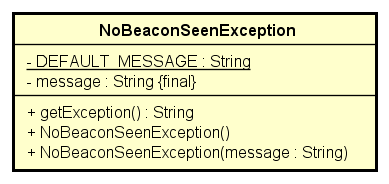
\includegraphics{img/NoBeaconSeenException.png}
        \caption{Classe NoBeaconSeenException}\label{fig:model::NoBeaconSeenException} 
    \end{figure}
    \begin{description}
\item[Nome:] \texttt{NoBeaconSeenException};
\item[Tipo:] Classe;
\item[Visibilità:] \texttt{public};
\item[Utilizzo:] Eccezione lanciata nel caso in cui venga richiesta una operazione che coinvolge l'utilizzo dei beacon ma non ne sono stati rilevati;
\item[Descrizione:] Classe che rappresenta l'eccezione lanciata nel caso in cui non siano rilevati beacon;
\item[Attributi:] \
\begin{itemize}
\item \texttt{- \underline{DEFAULT\_MESSAGE : String}}\\
Rappresenta il messaggio di default che viene mostrato quando non viene rilevato nessun beacon

\item \texttt{- message : String \{readOnly\}}\\
Rappresenta un messaggio qualsiasi quando non viene rilevato nessun beacon

\end{itemize}
\item[Metodi:] \
\begin{itemize}
\item \texttt{+ NoBeaconSeenException()}\\
Costruttore della classe di default
 \item \texttt{+ NoBeaconSeenException(message : String)}\\
Costruttore della classe che richiede un messaggio come parametro
 \begin{description}
\item[Argomenti:] \
\begin{itemize}
\item \texttt{message : String}\\
Questo parametro richiede che un messaggio di tipo  String\end{itemize}
\end{description}
\end{itemize}
\end{description}

\subsubsection{model::ServiceConnectionImp}

    \begin{figure}[H]
        \centering
        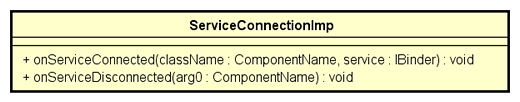
\includegraphics{img/ServiceConnectionImp.png}
        \caption{Classe ServiceConnectionImp}\label{fig:model::ServiceConnectionImp} 
    \end{figure}
    \begin{description}
\item[Nome:] \texttt{ServiceConnectionImp};
\item[Tipo:] Classe;
\item[Componenti delle librerie utilizzate:] \
\begin{itemize}
\item \texttt{android.content.ServiceConnection (Android)}.

\end{itemize}
\item[Visibilità:] \texttt{public};
\item[Utilizzo:] È utilizzata per comunicare con un'istanzza della classe BeaconManagerAdapter, per dare la possibilità di ridurre il periodo di scansione per la ricerca dei beacon e per mettere in pausa la scansione qualora l'applicazione venisse messa in background;
\item[Descrizione:] Classe che implementa android.content.ServiceConnection, utile al fine di comunicare con la classe che si occupa del rilevamento dei beacon;
\item[Metodi:] \
\begin{itemize}
\item \texttt{+ onServiceConnected(className : ComponentName, service : IBinder) : void}\\
Questo metodo permette di specificare determinate azioni nel momento in cui un servizio(Service) viene connesso ad un componente
 \begin{description}
\item[Argomenti:] \
\begin{itemize}
\item \texttt{className : ComponentName}\\
Questo parametro richiede il nome del servizio su cui si vuole eseguire la connessione\item \texttt{service : IBinder}\\
Questo parametro richiede l'IBinder del servizio con cui si vuole effettuare la connessione\end{itemize}
\end{description}
\item \texttt{+ onServiceDisconneted(className : ComponentName) : void}\\
Questo metodo permette di eseguire delle azioni nel momento in cui un servizio (Service) viene interrotto o termina in seguito ad un errore.
 \begin{description}
\item[Argomenti:] \
\begin{itemize}
\item \texttt{className : ComponentName}\\
Questo parametro richiede il nome del servizio che è stato interrotto o è terminato in seguito ad errori\end{itemize}
\end{description}
\end{itemize}
\end{description}

\subsubsection{model::beacon::BeaconManagerAdapter}

    \begin{figure}[H]
        \centering
        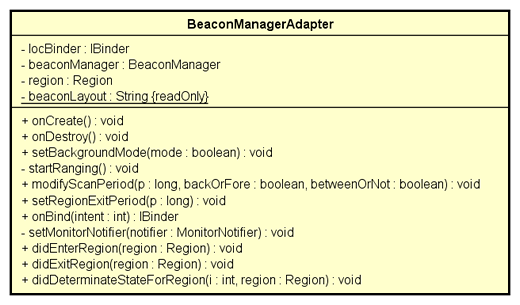
\includegraphics{img/BeaconManagerAdapter.png}
        \caption{Classe BeaconManagerAdapter}\label{fig:model::beacon::BeaconManagerAdapter} 
    \end{figure}
    \begin{description}
\item[Nome:] \texttt{BeaconManagerAdapter};
\item[Tipo:] Classe;
\item[Implementa:] \
\begin{itemize}
\item \texttt{BeaconRanger}.

\end{itemize}
\item[Componenti delle librerie utilizzate:] \
\begin{itemize}
\item \texttt{android.app.Service (Android)}.

\end{itemize}
\item[Visibilità:] \texttt{public};
\item[Utilizzo:] È utilizzata per rilevare i beacon;
\item[Descrizione:] Classe che si occupa del rilevamento dei beacon. Estende la classe android.app.Service e implementa le interfacce org.altbeacon.beacon.BeaconConsumer e org.altbeacon.beacon.startup.BootstrapNotifier;
\item[Attributi:] \
\begin{itemize}
\item \texttt{- \underline{beaconLayout : String}}\\
Rappresenta una stringa che identifica la marca del Beacon o del protocollo

\item \texttt{- beaconManager : BeaconManager}\\
Riferimento alla classe che permette di gestire il rilevamento dei beacon

\item \texttt{- locBinder : IBinder}\\
Riferimento al LocalBinder che detiene il collegamento con il Service

\item \texttt{- region : Region}\\
Rappresenta un criterio che serve ad eseguire il match con un beacon

\end{itemize}
\item[Metodi:] \
\begin{itemize}
\item \texttt{+ didDeterminateStateForRegion(i : int , region : Region) : void}\\
Metodo che determina se un dispositivo è presente all'interno di una Region
 \begin{description}
\item[Argomenti:] \
\begin{itemize}
\item \texttt{i : int }\\
Stato della Region che può essere MonitorNotifier.INSIDE o MonitorNotifier.OUTSIDE\item \texttt{region : Region}\\
Criterio che serve ad eseguire il match con un beacon\end{itemize}
\end{description}
\item \texttt{+ didEnterRegion(region : Region) : void}\\
Metodo che definisce delle azioni da eseguire nel momento in cui il dispositivo rileva uno o più beacon nella Region
 \begin{description}
\item[Argomenti:] \
\begin{itemize}
\item \texttt{region : Region}\\
Criterio che serve ad eseguire il match con un beacon\end{itemize}
\end{description}
\item \texttt{+ didExitRegion(region : Region) : void}\\
Metodo che definisce delle azioni da eseguire nel momento in cui il dispositivo non rileva più beacon nella Region
 \begin{description}
\item[Argomenti:] \
\begin{itemize}
\item \texttt{region : Region}\\
Criterio che serve ad eseguire il match con un beacon\end{itemize}
\end{description}
\item \texttt{+ modifyScanPeriod(p : long, backOrFore : boolean, betweenOrNot : boolean) : void}\\
Metodo che serve a modificare il periodo di scansione per il rilevamento dei beacon
 \begin{description}
\item[Argomenti:] \
\begin{itemize}
\item \texttt{p : long}\\
Periodo di scansione\item \texttt{backOrFore : boolean}\\
Parametro per decidere se cambiare il periodo di scansione in Foreground o in Background\item \texttt{betweenOrNot : boolean}\\
Parametro che serve a decidere se modificare il periodo di scansione o di non scansione\end{itemize}
\end{description}
\item \texttt{+ onBind(intent : Intent) : IBinder}\\
Metodo che serve a definire determinate azioni nel momento in cui una classe viene collegata ad un Service 
 \begin{description}
\item[Argomenti:] \
\begin{itemize}
\item \texttt{intent : Intent}\\
Intent del Service di cui  si vuole fare il collegamento  \end{itemize}
\end{description}
\item \texttt{+ onCreate() : void}\\
Metodo che inizializza i parametri della classe alla creaziione di un'istanza
 \item \texttt{+ onDestroy() : void}\\
Metodo che esegue le azioni necessarie alla distruzione del Service
 \item \texttt{+ setBackgroundMode(mode : boolean) : void}\\
Metodo per notificare al Service che l'applicazione sta andando in background 
 \begin{description}
\item[Argomenti:] \
\begin{itemize}
\item \texttt{mode : boolean}\\
Questo parametro serve per impostare se l'applicazione sta andando in background o no.\end{itemize}
\end{description}
\item \texttt{- setMonitorNotifier() : void}\\
Metodo che imposta il monitor che rileva le notifiche
 \item \texttt{+ setRegionExitPeriod(p : long) : void}\\
Metodo per impostare il periodo che determina l'uscita di un beacon da una Region
 \begin{description}
\item[Argomenti:] \
\begin{itemize}
\item \texttt{p : long}\\
Questo parametro richiede il periodo in millisecondi \end{itemize}
\end{description}
\item \texttt{- startRanging() : void}\\
Questo metodo serve per far partire il Ranging dei Beacon 
 \end{itemize}
\end{description}

\subsubsection{model::beacon::BeaconRanger}

    \begin{figure}[H]
        \centering
        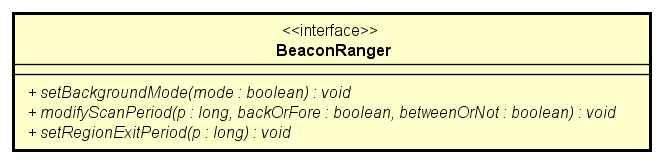
\includegraphics{img/BeaconRanger.png}
        \caption{Interfaccia BeaconRanger}\label{fig:model::beacon::BeaconRanger} 
    \end{figure}
    \begin{description}
\item[Nome:] \texttt{BeaconRanger};
\item[Tipo:] Interfaccia;
\item[Visibilità:] \texttt{public};
\item[Utilizzo:] È utilizzata al fine di rendere indipendente il rilevamento dei beacon dalla sua implementazione;
\item[Descrizione:] Interfaccia che espone tutti i metodi che possono essere invocati su di una classe che si occupa del rilevamento dei beacon ;
\item[Metodi:] \
\begin{itemize}
\item \texttt{+ modifyScanPeriod(p : long, backOrFore : boolean, betweenOrNot : boolean) : void}\\
Metodo che serve a modificare il periodo di scansione per il rilevamento dei beacon
 \begin{description}
\item[Argomenti:] \
\begin{itemize}
\item \texttt{p : long}\\
Periodo di scansione\item \texttt{backOrFore : boolean}\\
Parametro per decidere se cambiare il periodo di scansione in Foreground o in Background\item \texttt{betweenOrNot : boolean}\\
Parametro che serve a decidere se modificare il periodo di scansione o di non scansione\end{itemize}
\end{description}
\item \texttt{+ setBackgroundMode() : void}\\
Metodo per notificare al Service che l'applicazione sta andando in background 
 \item \texttt{+ setRegionExitPeriod() : void}\\
Metodo per impostare il periodo che determina l'uscita di un beacon da una Region
 \end{itemize}
\end{description}

\subsubsection{model::beacon::LocalBinder}

    \begin{figure}[H]
        \centering
        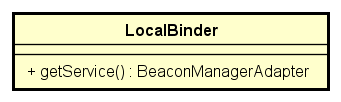
\includegraphics{img/LocalBinder.png}
        \caption{Classe LocalBinder}\label{fig:model::beacon::LocalBinder} 
    \end{figure}
    \begin{description}
\item[Nome:] \texttt{LocalBinder};
\item[Tipo:] Classe;
\item[Componenti delle librerie utilizzate:] \
\begin{itemize}
\item \texttt{android.os.Binder (Android)}.

\end{itemize}
\item[Visibilità:] \texttt{public};
\item[Utilizzo:] È utilizzata per la comunicazione tra i processi;
\item[Descrizione:] Classe definita per permettere la comunicazione tra processi (IPC), in questo caso permette di comunicare con i metodi pubblici definiti internamente ad una classe Service. Estende la classe android.os.Binder;
\item[Metodi:] \
\begin{itemize}
\item \texttt{+ getService() : BeaconManagerAdapter}\\
Questo metodo restituisce il riferimento al Service BeaconManagerAdapter
 \end{itemize}
\end{description}

\subsubsection{model::beacon::Logger}

    \begin{figure}[H]
        \centering
        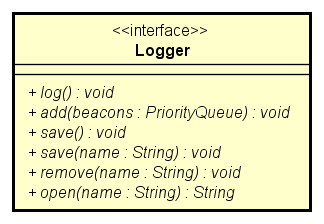
\includegraphics{img/Logger.png}
        \caption{Interfaccia Logger}\label{fig:model::beacon::Logger} 
    \end{figure}
    \begin{description}
\item[Nome:] \texttt{Logger};
\item[Tipo:] Interfaccia;
\item[Visibilità:] \texttt{public};
\item[Utilizzo:] È necessaria per rendere indipendente l'utilizzo di un logger dalla sua implementazione;
\item[Descrizione:] Interfaccia che espone i metodi utili per accedere alle funzionalità di un logger;
\item[Metodi:] \
\begin{itemize}
\item \texttt{+ \textit{add(beacons : PriorityQueue<MyBeacon>) : void}}\\
Metodo che aggiunge all'insieme di informazioni di beacon già eventualmente presenti le informazioni riguardanti i beacon passati in ingresso
 \begin{description}
\item[Argomenti:] \
\begin{itemize}
\item \texttt{beacons : PriorityQueue<MyBeacon>}\\
Insieme dei beacon di cui salvare le informazioni.\end{itemize}
\end{description}
\item \texttt{+ \textit{log() : void}}\\
Metodo che salva le informazioni contenute nell'oggetto su di un file
 \item \texttt{+ \textit{open(name : String) : String}}\\
Metodo che, dato il nome di un file di log, ritorna l'informazione in esso contenuta sotto forma di stringa
 \begin{description}
\item[Argomenti:] \
\begin{itemize}
\item \texttt{name : String}\\
Nome del file di log da cui reperire le informazioni\end{itemize}
\end{description}
\item \texttt{+ \textit{remove(name : String) : void}}\\
Metodo per la rimozione di un log precedentemente salvato
 \begin{description}
\item[Argomenti:] \
\begin{itemize}
\item \texttt{name : String}\\
Nome del log da rimuovere\end{itemize}
\end{description}
\item \texttt{+ \textit{save(filename : String) : void}}\\
Metodo che salva le informazioni contenute nell'oggetto su di un file con nome uguale alla stringa passata come parametro
 \begin{description}
\item[Argomenti:] \
\begin{itemize}
\item \texttt{filename : String}\\
Nome da dare al file.\end{itemize}
\end{description}
\end{itemize}
\end{description}

\subsubsection{model::beacon::LoggerImp}

    \begin{figure}[H]
        \centering
        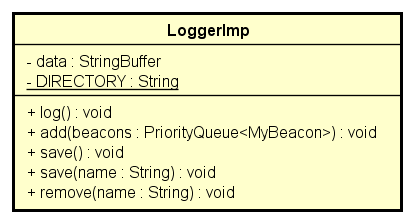
\includegraphics{img/LoggerImp.png}
        \caption{Classe LoggerImp}\label{fig:model::beacon::LoggerImp} 
    \end{figure}
    \begin{description}
\item[Nome:] \texttt{LoggerImp};
\item[Tipo:] Classe;
\item[Implementa:] \
\begin{itemize}
\item \texttt{Logger}.

\end{itemize}
\item[Visibilità:] \texttt{public};
\item[Utilizzo:] È utilizzata per raccogliere i dati dei beacon che devono essere salvati e per salvare tali dati in un file;
\item[Descrizione:] Classe che implementa Logger, per la gestione di un log;
\item[Attributi:] \
\begin{itemize}
\item \texttt{- data : StringBuffer}\\
Rappresenta il contenuto di un log

\item \texttt{- \underline{directory : String \{readOnly\}}}\\
Path della directory in cui vengono salvati i log

\end{itemize}
\item[Metodi:] \
\begin{itemize}
\item \texttt{+ add(beacons : PriorityQueue<MyBeacon>) : void}\\
Metodo che aggiunge all'insieme di informazioni di beacon già eventualmente presenti le informazioni riguardanti i beacon passati in ingresso
 \begin{description}
\item[Argomenti:] \
\begin{itemize}
\item \texttt{beacons : PriorityQueue<MyBeacon>}\\
Questo parametro richiede una lista di beacons\end{itemize}
\end{description}
\item \texttt{+ \underline{getDirectory() : String}}\\
Metodo che restituisce il path della directory in cui vengono salvati i log
 \item \texttt{+ log() : void}\\
Metodo che salva le informazioni contenute nell'oggetto su di un file
 \item \texttt{+ open(name : String) : String}\\
Metodo che, dato il nome di un log, ritorna sotto forma di stringa l'informazione in esso contenuta
 \begin{description}
\item[Argomenti:] \
\begin{itemize}
\item \texttt{name : String}\\
Nome del log da cui reperire le informazioni\end{itemize}
\end{description}
\item \texttt{+ remove(name : String) : void}\\
Metodo per la rimozione di un log precedentemente salvato
 \begin{description}
\item[Argomenti:] \
\begin{itemize}
\item \texttt{name : String}\\
Nome del log da rimuovere\end{itemize}
\end{description}
\item \texttt{+ save(name : String) : void}\\
Metodo che salva le informazioni contenute nell'oggetto su di un file con nome uguale alla stringa passata come parametro
 \begin{description}
\item[Argomenti:] \
\begin{itemize}
\item \texttt{name : String}\\
Nome del file sul quale salvare il log\end{itemize}
\end{description}
\item \texttt{+ save() : void}\\
Metodo che salva le informazioni contenute nell'oggetto su di un file
 \end{itemize}
\end{description}

\subsubsection{model::beacon::MyBeacon}

    \begin{figure}[H]
        \centering
        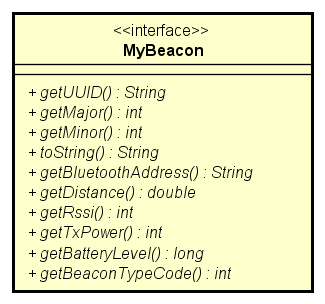
\includegraphics{img/MyBeacon.png}
        \caption{Interfaccia MyBeacon}\label{fig:model::beacon::MyBeacon} 
    \end{figure}
    \begin{description}
\item[Nome:] \texttt{MyBeacon};
\item[Tipo:] Interfaccia;
\item[Visibilità:] \texttt{public};
\item[Utilizzo:] È utilizzata al fine di rendere indipendente l'accesso alle informazioni dei beacon da come questi sono rappresentati. È utile inoltre nel caso in cui non si voglia, in futuro, utilizzare più la libreria Altbeacon. Utilizzando questa interfaccia nel Model infatti, in caso di un cambiamento, non sarà necessario cambiare altre parti di model all'infuori del package beacon, a meno di un ampliamento delle funzionalità;
\item[Descrizione:] Interfaccia che espone tutti i metodi che possono essere invocati su di un beacon gestito all'interno della nostra applicazione. Estende l'interfaccia java.io.Serializable;
\item[Metodi:] \
\begin{itemize}
\item \texttt{+ \textit{getBatteryLevel() : long}}\\
Metodo che ritorna il livello di batteria del beacon rilevato
 \item \texttt{+ \textit{getBeaconTypeCode() : int}}\\
Metodo che ritorna il codice rappresentante il tipo di beacon che è stato rilevato
 \item \texttt{+ \textit{getBluetoothAddress() : String}}\\
Metodo che ritorna l'indirizzo Bluetooth del beacon
 \item \texttt{+ \textit{getDistance() : double}}\\
Metodo che ritorna la distanza del beacon dal dispositivo che lo ha rilevato
 \item \texttt{+ \textit{getMajor() : int}}\\
Metodo che ritorna l'identificativo Major del beacon
 \item \texttt{+ \textit{getMinor() : int}}\\
Metodo che ritorna l'identificativo Minor del beacon
 \item \texttt{+ \textit{getRssi() : int}}\\
Metodo che ritorna la potenza ricevuta del segnale del beacon
 \item \texttt{+ \textit{getTxPower() : int}}\\
Metodo che ritorna la potenza di trasmissione del beacon
 \item \texttt{+ \textit{getUUID() : String}}\\
Metodo che ritorna l'identificativo UUID del beacon
 \end{itemize}
\end{description}

\subsubsection{model::beacon::MyBeaconImp}

    \begin{figure}[H]
        \centering
        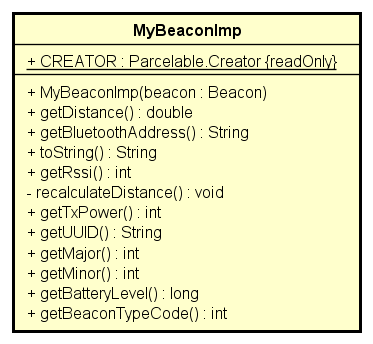
\includegraphics{img/MyBeaconImp.png}
        \caption{Classe MyBeaconImp}\label{fig:model::beacon::MyBeaconImp} 
    \end{figure}
    \begin{description}
\item[Nome:] \texttt{MyBeaconImp};
\item[Tipo:] Classe;
\item[Implementa:] \
\begin{itemize}
\item \texttt{MyBeacon}.

\end{itemize}
\item[Componenti delle librerie utilizzate:] \
\begin{itemize}
\item \texttt{org.altbeacon.beacon.Beacon (AltBeacon)}.

\end{itemize}
\item[Visibilità:] \texttt{public};
\item[Utilizzo:] È utilizzata per accedere alle informazioni di un beacon sfruttando la classe org.altbeacon.beacon.Beacon, adattandola alle necessità dell'applicazione;
\item[Descrizione:] Classe che implementa l'interfaccia MyBeacon. Offre tutti i metodi per accedere alle informazioni di un beacon. Estende la classe org.altbeacon.beacon.Beacon;
\item[Attributi:] \
\begin{itemize}
\item \texttt{- \underline{CREATOR : List<NavigationInformationImp,Parcelable.Creator<MyBeaconImp> \{readOnly\}}}\\
Attributo richiesto per rendere la classe Parcelable

\end{itemize}
\item[Metodi:] \
\begin{itemize}
\item \texttt{+ getBatteryLevel() : long}\\
Metodo che ritorna il livello di batteria del beacon rilevato
 \item \texttt{+ getBeaconTypeCode() : int}\\
Metodo che ritorna il codice rappresentante il tipo di beacon che è stato rilevato
 \item \texttt{+ getBluetoothAddress() : String}\\
Metodo che ritorna l'indirizzo Bluetooth del beacon
 \item \texttt{+ getDistance() : double}\\
Metodo che ritorna la distanza del beacon dal dispositivo che lo ha rilevato
 \item \texttt{+ getMajor() : int}\\
Metodo che ritorna l'identificativo Major del beacon
 \item \texttt{+ getMinor() : int}\\
Metodo che ritorna l'identificativo Minor del beacon
 \item \texttt{+ getRssi() : int}\\
Metodo che ritorna la potenza ricevuta del segnale del beacon
 \item \texttt{+ getTxPower() : int}\\
Metodo che ritorna la potenza di trasmissione del beacon
 \item \texttt{+ getUUID() : String}\\
Metodo che ritorna l'identificativo UUID del beacon
 \item \texttt{+ MyBeaconImp(beacon : Beacon)}\\
Costruttore della classe
 \begin{description}
\item[Argomenti:] \
\begin{itemize}
\item \texttt{beacon : Beacon}\\
Questo parametro richiede un beacon\end{itemize}
\end{description}
\item \texttt{+ recalculateDistance() : void}\\
Questo metodo permette di ricalcolare la distanza tra il beacon e il dispositivo
 \item \texttt{+ toString() : String}\\
Questo metodo permette di fornire una conversione di MyBeaconImp a tipo String
 \end{itemize}
\end{description}

\subsubsection{model::beacon::MyDistanceCalculator}

    \begin{figure}[H]
        \centering
        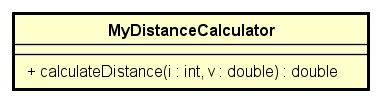
\includegraphics{img/MyDistanceCalculator.png}
        \caption{Classe MyDistanceCalculator}\label{fig:model::beacon::MyDistanceCalculator} 
    \end{figure}
    \begin{description}
\item[Nome:] \texttt{MyDistanceCalculator};
\item[Tipo:] Classe;
\item[Componenti delle librerie utilizzate:] \
\begin{itemize}
\item \texttt{org.altbeacon.beacon.distance.DistanceCalculator (AltBeacon)}.

\end{itemize}
\item[Visibilità:] \texttt{public};
\item[Utilizzo:] È utilizzata per calcolare la distanza di un beacon dal dispositivo che lo ho rilevato;
\item[Descrizione:] Classe che implementa l'intefaccia org.altbeacon.beacon.distance.DistanceCaluclator;
\item[Metodi:] \
\begin{itemize}
\item \texttt{+ calculateDistance(i : int, v : double) : double}\\
Questo metodo calcola la distanza di un beacon dal dispositivo
 \begin{description}
\item[Argomenti:] \
\begin{itemize}
\item \texttt{i : int}\\
Questo parametro richiede la potenza del beacon di cui si vuole calcolare la distanza\item \texttt{v : double}\\
Questo parametro richiede il valore rssi del beacon di cui si vuole calcolare la distanza\end{itemize}
\end{description}
\end{itemize}
\end{description}

\subsubsection{model::compass::Compass}

    \begin{figure}[H]
        \centering
        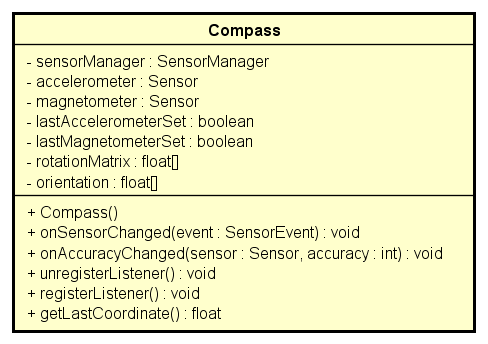
\includegraphics{img/Compass.png}
        \caption{Classe Compass}\label{fig:model::compass::Compass} 
    \end{figure}
    \begin{description}
\item[Nome:] \texttt{Compass};
\item[Tipo:] Classe;
\item[Componenti delle librerie utilizzate:] \
\begin{itemize}
\item \texttt{android.hardware.Sensor (Android)};

\item \texttt{android.hardware.SensorEventListener (Android)};

\item \texttt{android.hardware.SensorManager (Android)}.

\end{itemize}
\item[Visibilità:] \texttt{public};
\item[Utilizzo:] È utilizzata per calcolare e restituire l'orientamento del dispositivo;
\item[Descrizione:] Classe che si occupa di gestire i dati ricavabili dai sensori e calcolare l'orientamento del device;
\item[Attributi:] \
\begin{itemize}
\item \texttt{- accelerometer : Sensor}\\
Sensore che misura l'accellerazione del device sui tre assi fisici

\item \texttt{- lastAccelerometerSet : boolean}\\
variabile di guardia per accertarsi il reperimento di almeno un dato dall'accellerometro

\item \texttt{- lastMagnetometerSet : boolean}\\
variabile di guardia per accertarsi il reperimento di almeno un dato dal magnetometro

\item \texttt{- magnetometer : Sensor}\\
Sensore che misura il campo magnetico per i tre assi fisici

\item \texttt{- orientation : float[]}\\
gradi di orientamento sui tre assi fisici

\item \texttt{- rotationMatrix : float[]}\\
matrice di rotazione ottenuta dai dati rilevati dai sensori

\item \texttt{- sensorManager : SensorManager}\\
oggetto fornito dal sistema Android per ottenere le istanze dei sensori

\end{itemize}
\item[Metodi:] \
\begin{itemize}
\item \texttt{+ Compass()}\\
Costruttore della classe Compass
 \item \texttt{+ getLastCoordinate() : float}\\
Metodo che restituisce l'ultimo dato calcolato dai dati ricavati dai sensori che indica l'orientamento del dispositivo.
 \item \texttt{+ onAccuracyChanged(sensor : Sensor, accuracy : int) : void}\\
Metodo che viene chiamato nel caso in cui l'accuratezza dei sensori è cambiata. Attualmente non viene utilizzato dall'applicativo
 \begin{description}
\item[Argomenti:] \
\begin{itemize}
\item \texttt{sensor : Sensor}\\
Riferimento al sensore che ha scatenato l'evento\item \texttt{accuracy : int}\\
Nuova accuratezza impostata al sensore \end{itemize}
\end{description}
\item \texttt{+ onSensorChanged(event : SensorEvent) : void}\\
Metodo invocato ad ogni evento generato dai sensori attivi di Compass. Fornisce quindi i dati misurati dal sensore e elaborandoli ne ricava l'orientamento del device
 \begin{description}
\item[Argomenti:] \
\begin{itemize}
\item \texttt{event : SensorEvent}\\
Rappresenta un evento scatenato da un sensore del dispositivo e detiene al suo interno tutti i dati rilevati da quel sensore\end{itemize}
\end{description}
\item \texttt{+ registerListener() : void}\\
Metodo che permette all'oggetto Compass di ricevere dati dai sensori e quindi accenderli
 \item \texttt{+ unregisterListener() : void}\\
Metodo che permette all'oggetto Compass di smettere di ricevere dati dai sensori e quindi spegnerli
 \end{itemize}
\end{description}

\subsubsection{model::dataaccess::dao::BuildingContract}

    \begin{figure}[H]
        \centering
        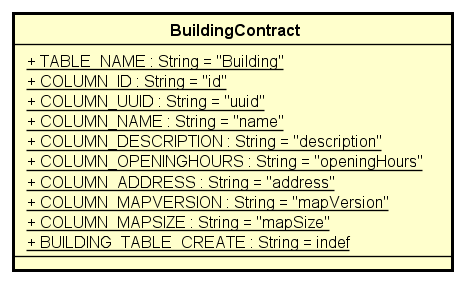
\includegraphics{img/BuildingContract.png}
        \caption{Classe BuildingContract}\label{fig:model::dataaccess::dao::BuildingContract} 
    \end{figure}
    \begin{description}
\item[Nome:] \texttt{BuildingContract};
\item[Tipo:] Classe;
\item[Visibilità:] \texttt{public};
\item[Utilizzo:] Utilizzata per reperire le informazioni corrette della tabella Building del database locale;
\item[Descrizione:] Classe che contiene le informazioni corrette della tabella Building del database locale;
\item[Attributi:] \
\begin{itemize}
\item \texttt{+ \underline{BUILDING\_TABLE\_CREATE : String \{readOnly\}}}\\
Query per la creazione della tabella

\item \texttt{+ \underline{COLUMN\_ADDRESS : String \{readOnly\}}}\\
Valore della colonna address. Valore di default "address"

\item \texttt{+ \underline{COLUMN\_DESCRIPTION : String \{readOnly\}}}\\
Valore della colonna description. Valore di default "description"

\item \texttt{+ \underline{COLUMN\_ID : String \{readOnly\}}}\\
Valore della colonna id. Valore di default "id"

\item \texttt{+ \underline{COLUMN\_MAPVERSION : String \{readOnly\}}}\\
Valore della colonna mapVersion. Valore di default "mapVersion"

\item \texttt{+ \underline{COLUMN\_NAME : String \{readOnly\}}}\\
name

\item \texttt{+ \underline{COLUMN\_OPENINGHOURS : String \{readOnly\}}}\\
Valore della colonna openingHours. Valore di default "openingHours"

\item \texttt{+ \underline{COLUMN\_UUID : String \{readOnly\}}}\\
Valore della colonna uuid. Valore di default "uuid"

\item \texttt{+ \underline{TABLE\_NAME : String \{readOnly\}}}\\
Nome della tabella.Valore di default "Building"

\end{itemize}
\end{description}

\subsubsection{model::dataaccess::dao::BuildingDao}

    \begin{figure}[H]
        \centering
        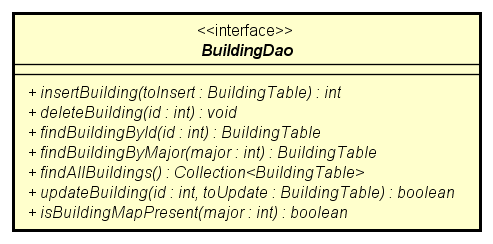
\includegraphics{img/BuildingDao.png}
        \caption{Interfaccia BuildingDao}\label{fig:model::dataaccess::dao::BuildingDao} 
    \end{figure}
    \begin{description}
\item[Nome:] \texttt{BuildingDao};
\item[Tipo:] Interfaccia;
\item[Visibilità:] \texttt{public};
\item[Utilizzo:] Viene utilizzata per rendere indipendenti l'invocazioni dei metodi per effettuare le operazioni CRUD sulla tabella "Building" del database locale dalla loro implementazione;
\item[Descrizione:] Interfaccia che espone i metodi per un DAO per accedere alla tabella "Building" del database locale;
\item[Metodi:] \
\begin{itemize}
\item \texttt{+ \textit{deleteBuilding(id : int) : void}}\\
Metodo che permette la rimozione delle informazioni di un edificio dalla tabella "Building" del database locale 
 \begin{description}
\item[Argomenti:] \
\begin{itemize}
\item \texttt{id : int}\\
Identificativo dell'edificio di cui rimuovere le informazioni dal database locale\end{itemize}
\end{description}
\item \texttt{+ \textit{findAllBuildings() : Collection<BuildingTable>}}\\
Metodo che viene utilizzato per recuperare le informazioni di tutti gli edifici presenti nella tabella "Building" del database locale
 \item \texttt{+ \textit{findBuildingById(id : int) : BuildingTable}}\\
Metodo che viene utilizzato per recuperare le informazioni di tutti gli edifici presenti nella tabella "Building" del database locale
 \begin{description}
\item[Argomenti:] \
\begin{itemize}
\item \texttt{id : int}\\
Identificativo dell'edificio di cui recuperare le informazioni\end{itemize}
\end{description}
\item \texttt{+ \textit{findBuildingByMajor(major : int) : BuildingTable}}\\
Metodo per recuperare le informazioni di un edificio dal database locale tramite il suo major, sotto forma di oggetto BuildingTable
 \begin{description}
\item[Argomenti:] \
\begin{itemize}
\item \texttt{major : int}\\
Major identificante l'edificio che deve essere recuperato dal database\end{itemize}
\end{description}
\item \texttt{+ \textit{insertBuilding(toInsert : BuildingTable) : int}}\\
Metodo che permette l'inserimento delle informazioni di un edificio in una entry della tabella "Building" del database locale
 \begin{description}
\item[Argomenti:] \
\begin{itemize}
\item \texttt{toInsert : BuildingTable}\\
Oggetto di tipo BuildingTable che contiene le informazioni dell'edificio\end{itemize}
\end{description}
\item \texttt{+ \textit{isBuildingMapPresent(major : int) : boolean}}\\
Metodo per verificare la presenza nel database locale delle informazioni di un edificio
 \begin{description}
\item[Argomenti:] \
\begin{itemize}
\item \texttt{major : int}\\
major dell'edificio\end{itemize}
\end{description}
\item \texttt{+ \textit{updateBuilding(id : int, toUpdate : BuildingTable) : boolean}}\\
Metodo per aggiornare le informazioni di un edificio nella tabella "Building" del database locale
 \begin{description}
\item[Argomenti:] \
\begin{itemize}
\item \texttt{id : int}\\
Identificativo dell'edificio di cui aggiornare le informazioni\item \texttt{toUpdate : BuildingTable}\\
Oggetto che contiene le informazioni aggiornate dell'edificio\end{itemize}
\end{description}
\end{itemize}
\end{description}

\subsubsection{model::dataaccess::dao::BuildingTable}

    \begin{figure}[H]
        \centering
        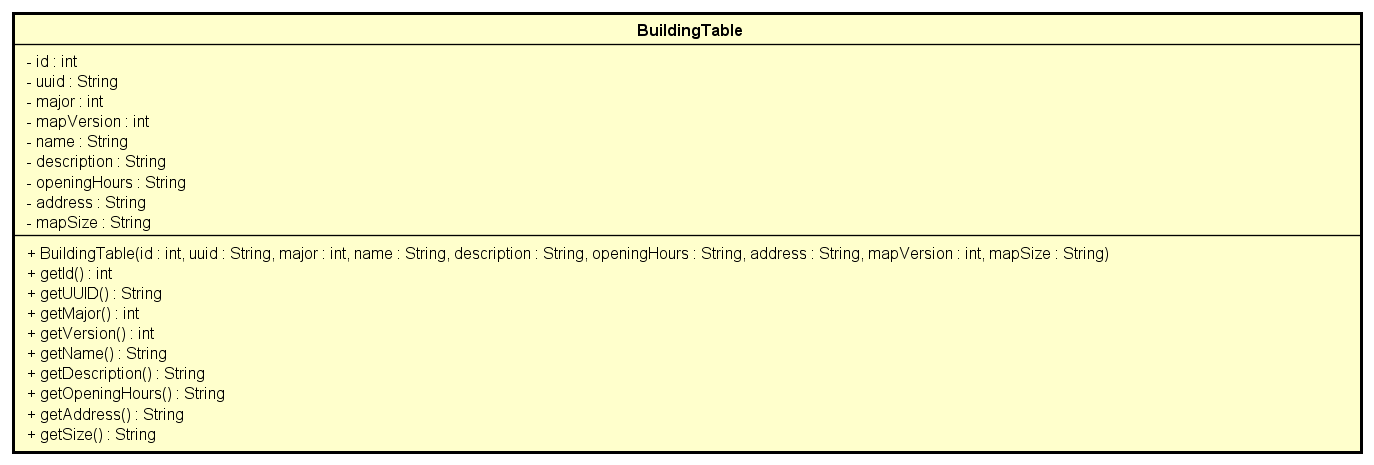
\includegraphics{img/BuildingTable.png}
        \caption{Classe BuildingTable}\label{fig:model::dataaccess::dao::BuildingTable} 
    \end{figure}
    \begin{description}
\item[Nome:] \texttt{BuildingTable};
\item[Tipo:] Classe;
\item[Visibilità:] \texttt{public};
\item[Utilizzo:] Viene utilizzata per recuperare le informazioni di una ennupla della tabella Building del database locale ;
\item[Descrizione:] Classe che rappresenta una ennupla della tabella Building del database locale;
\item[Attributi:] \
\begin{itemize}
\item \texttt{- address : String}\\
Indirizzo dell'edificio

\item \texttt{- description : String}\\
Descrizione dell'edificio

\item \texttt{- id : int}\\
Identificativo dell'edificio

\item \texttt{- major : int}\\
Major dell'edificio

\item \texttt{- mapSize : String}\\
Dimensione della mappa (in MB)

\item \texttt{- mapVersion : int}\\
Versione corrente della mappa

\item \texttt{- name : String}\\
Nome dell'edificio

\item \texttt{- openingHours : String}\\
Orario dell'apertura dell'edificio

\item \texttt{- uuid : String}\\
Identificativo dell'applicazione

\end{itemize}
\item[Metodi:] \
\begin{itemize}
\item \texttt{+ BuildingTable(id : int, uuid : String, major : int, name : String, description : String, openingHours : String, address : String, mapVersion : int, mapSize : String)}\\
Costruttore della classe BuildingTable
 \begin{description}
\item[Argomenti:] \
\begin{itemize}
\item \texttt{id : int}\\
Identificativo numerico dell'oggetto BuildingTable\item \texttt{uuid : String}\\
Identificativo univoco\item \texttt{major : int}\\
Major dell'edificio\item \texttt{name : String}\\
Nome dell'edificio mappato\item \texttt{description : String}\\
Descrizione dell'edificio mappato\item \texttt{openingHours : String}\\
Orari di apertura dell'edificio mappato\item \texttt{address : String}\\
Indirizzo dell'edificio mappato\item \texttt{mapVersion : int}\\
Versione della mappa\item \texttt{mapSize : String}\\
Dimensione della mappa (espressa in MB)\end{itemize}
\end{description}
\item \texttt{+ getAddress() : String}\\
Metodo che ritorna l'indirizzo dell'edificio
 \item \texttt{+ getDescription() : String}\\
Metodo che ritorna la descrizione dell'edificio
 \item \texttt{+ getId() : int}\\
Metodo che ritorna l'identificativo dell'edificio
 \item \texttt{+ getMajor() : int}\\
Metodo che ritorna il major dell'edificio
 \item \texttt{+ getName() : String}\\
Metodo che ritorna il nome dell'edificio
 \item \texttt{+ getOpeningHours() : String}\\
Metodo che ritorna l'orario di apertura dell'edificio
 \item \texttt{+ getSize() : String}\\
Metodo che ritorna la dimensione della mappa (in MB)
 \item \texttt{+ getUUID() : String}\\
Metodo che ritorna l'identificativo dell'applicazione
 \item \texttt{+ getVersion() : int}\\
Metodo che ritorna la versione della mappa dell'edificio
 \end{itemize}
\end{description}

\subsubsection{model::dataaccess::dao::CategoryContract}

    \begin{figure}[H]
        \centering
        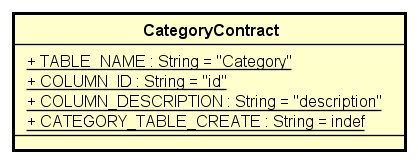
\includegraphics{img/CategoryContract.png}
        \caption{Classe CategoryContract}\label{fig:model::dataaccess::dao::CategoryContract} 
    \end{figure}
    \begin{description}
\item[Nome:] \texttt{CategoryContract};
\item[Tipo:] Classe;
\item[Visibilità:] \texttt{public};
\item[Utilizzo:] Utilizzata per reperire le informazioni corrette della tabella Category del database locale;
\item[Descrizione:] Classe che contiene le informazioni corrette della tabella Category del database locale;
\item[Attributi:] \
\begin{itemize}
\item \texttt{+ \underline{CATEGORY\_TABLE\_CREATE : String \{readOnly\}}}\\
Query per la creazione della tabella

\item \texttt{+ \underline{COLUMN\_DESCRIPTION : String \{readOnly\}}}\\
Valore della colonna description. Valore di default "description"

\item \texttt{+ \underline{COLUMN\_ID : String \{readOnly\}}}\\
Valore della colonna id. Valore di default "id"

\item \texttt{+ \underline{TABLE\_NAME : String \{readOnly\}}}\\
Nome della tabella. Valore di default "Category"

\end{itemize}
\end{description}

\subsubsection{model::dataaccess::dao::CategoryDao}

    \begin{figure}[H]
        \centering
        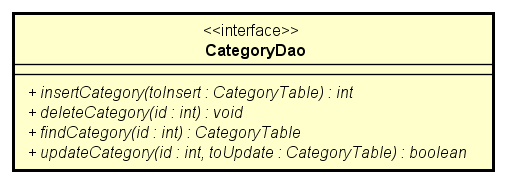
\includegraphics{img/CategoryDao.png}
        \caption{Interfaccia CategoryDao}\label{fig:model::dataaccess::dao::CategoryDao} 
    \end{figure}
    \begin{description}
\item[Nome:] \texttt{CategoryDao};
\item[Tipo:] Interfaccia;
\item[Visibilità:] \texttt{public};
\item[Utilizzo:] Viene utilizzata per rendere indipendenti l'invocazioni dei metodi per effettuare le operazioni CRUD sulla tabella "Category" del database locale dalla loro implementazione;
\item[Descrizione:] .Interfaccia che espone i metodi per un DAO per accedere alla tabella "Category" del database locale;
\item[Metodi:] \
\begin{itemize}
\item \texttt{+ \textit{deleteCategory(id : int) : void}}\\
Metodo che permette la rimozione delle informazioni di un edificio dalla tabella "Category" del database locale
 \begin{description}
\item[Argomenti:] \
\begin{itemize}
\item \texttt{id : int}\\
Identificativo della categoria da rimuovere dal database locale\end{itemize}
\end{description}
\item \texttt{+ \textit{findCategory(id : int) : CategoryTable}}\\
Metodo per recuperare le informazioni di una categoria dal database locale tramite il suo identificativo, sotto forma di oggetto CategoryTable
 \begin{description}
\item[Argomenti:] \
\begin{itemize}
\item \texttt{id : int}\\
Identificativo della categoria di cui recuperare le informazioni\end{itemize}
\end{description}
\item \texttt{+ \textit{insertCategory(toInsert : CategoryTable) : int}}\\
Metodo che permette l'inserimento di una categoria nella tabella "Category" del database locale
 \begin{description}
\item[Argomenti:] \
\begin{itemize}
\item \texttt{toInsert : CategoryTable}\\
Oggetto di tipo CategoryTable che contiene le informazioni della categoria\end{itemize}
\end{description}
\item \texttt{+ \textit{updateCategory(id : int, toUpdate : CategoryTable) : boolean}}\\
Metodo per aggiornare le informazioni di una categoria nella tabella "Category" del database locale
 \begin{description}
\item[Argomenti:] \
\begin{itemize}
\item \texttt{id : int}\\
Identificativo della categoria di cui aggiornare le informazioni\item \texttt{toUpdate : CategoryTable}\\
Oggetto che contiene le informazioni aggiornate della categoria\end{itemize}
\end{description}
\end{itemize}
\end{description}

\subsubsection{model::dataaccess::dao::CategoryTable}

    \begin{figure}[H]
        \centering
        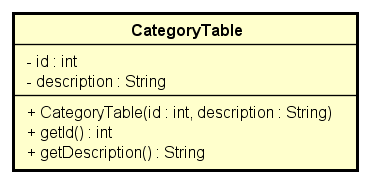
\includegraphics{img/CategoryTable.png}
        \caption{Classe CategoryTable}\label{fig:model::dataaccess::dao::CategoryTable} 
    \end{figure}
    \begin{description}
\item[Nome:] \texttt{CategoryTable};
\item[Tipo:] Classe;
\item[Visibilità:] \texttt{public};
\item[Utilizzo:] Viene utilizzata per recuperare le informazioni di una ennupla della tabella Category del database locale ;
\item[Descrizione:] Classe che rappresenta una ennupla della tabella Category del database locale;
\item[Attributi:] \
\begin{itemize}
\item \texttt{- description : String}\\
Nome della categoria

\item \texttt{- id : int}\\
Identificativo numerico dell'oggetto CategoryTable

\end{itemize}
\item[Metodi:] \
\begin{itemize}
\item \texttt{+ CategoryTable(id : int, description : String)}\\
Costruttore della classe CategoryTable
 \begin{description}
\item[Argomenti:] \
\begin{itemize}
\item \texttt{id : int}\\
Identificativo numerico dell'oggetto CategoryTable\item \texttt{description : String}\\
Nome della categoria\end{itemize}
\end{description}
\item \texttt{+ getDescription() : String}\\
Metodo che restituisce il nome della categoria
 \item \texttt{+ getId() : int}\\
Metodo che restituisce l'identificativo numerico dell'oggetto CategoryTable
 \end{itemize}
\end{description}

\subsubsection{model::dataaccess::dao::CursorConverter}

    \begin{figure}[H]
        \centering
        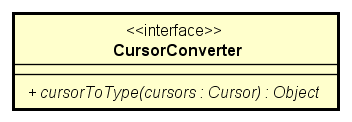
\includegraphics{img/CursorConverter.png}
        \caption{Interfaccia CursorConverter}\label{fig:model::dataaccess::dao::CursorConverter} 
    \end{figure}
    \begin{description}
\item[Nome:] \texttt{CursorConverter};
\item[Tipo:] Interfaccia;
\item[Componenti delle librerie utilizzate:] \
\begin{itemize}
\item \texttt{android.database.Cursor (Android)}.

\end{itemize}
\item[Visibilità:] \texttt{public};
\item[Utilizzo:] È utilizzata per rendere definire una unica firma per la conversione delle informazioni prese dal database in oggetti;
\item[Descrizione:] Interfaccia base per la conversione di un Cursor in un oggetto;
\item[Metodi:] \
\begin{itemize}
\item \texttt{+ \textit{cursorToType(cursor : Cursor) : Object}}\\
Metodo che viene utilizzato per convertire il risultato di una qury sul database locale in un oggetto
 \begin{description}
\item[Argomenti:] \
\begin{itemize}
\item \texttt{cursor : Cursor}\\
Risultato della query sul database locale\end{itemize}
\end{description}
\end{itemize}
\end{description}

\subsubsection{model::dataaccess::dao::DaoFactoryHelper}

    \begin{figure}[H]
        \centering
        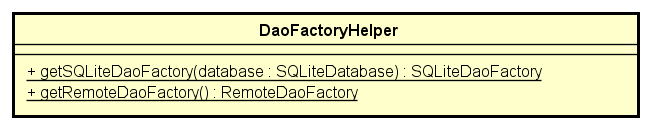
\includegraphics{img/DaoFactoryHelper.png}
        \caption{Classe DaoFactoryHelper}\label{fig:model::dataaccess::dao::DaoFactoryHelper} 
    \end{figure}
    \begin{description}
\item[Nome:] \texttt{DaoFactoryHelper};
\item[Tipo:] Classe;
\item[Visibilità:] \texttt{public};
\item[Utilizzo:] Viene utilizzata per ottenere un'istanza di SQLiteDaoFactory o di RemoteDaoFactory;
\item[Descrizione:] Classe che rappresenta un aiutante per ottenere un'istanza di una delle due Factory di DAO (locali o remoti);
\item[Metodi:] \
\begin{itemize}
\item \texttt{+ \underline{getRemoteDaoFactory() : RemoteDaoFactory}}\\
Metodo che viene utilizzato per ottenere un'istanza di RemoteDaoFactory
 \item \texttt{+ \underline{getSQLiteDaoFactory(database : SQLiteDatabase) : SQLiteDaoFactory}}\\
Metodo che viene utilizzato per ottenere un'istanza di SQLiteDaoFactory
 \begin{description}
\item[Argomenti:] \
\begin{itemize}
\item \texttt{database : SQLiteDatabase}\\
Il database locale\end{itemize}
\end{description}
\end{itemize}
\end{description}

\subsubsection{model::dataaccess::dao::EdgeContract}

    \begin{figure}[H]
        \centering
        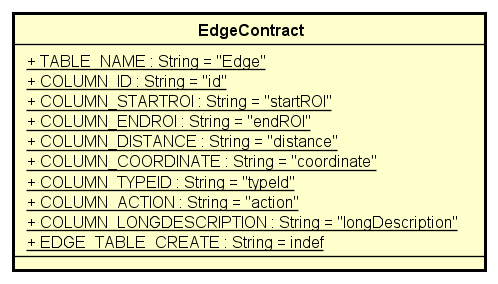
\includegraphics{img/EdgeContract.png}
        \caption{Classe EdgeContract}\label{fig:model::dataaccess::dao::EdgeContract} 
    \end{figure}
    \begin{description}
\item[Nome:] \texttt{EdgeContract};
\item[Tipo:] Classe;
\item[Visibilità:] \texttt{public};
\item[Utilizzo:] Utilizzata per reperire le informazioni corrette della tabella Edge del database locale;
\item[Descrizione:] Classe che contiene le informazioni corrette della tabella Edge del database locale;
\item[Attributi:] \
\begin{itemize}
\item \texttt{+ \underline{COLUMN\_ACTION : String \{readOnly\}}}\\
Valore della colonna action. Valore di default "action"

\item \texttt{+ \underline{COLUMN\_COORDINATE : String \{readOnly\}}}\\
Valore della colonna coordinate. Valore di default "coordinate"

\item \texttt{+ \underline{COLUMN\_DISTANCE : String \{readOnly\}}}\\
Valore della colonna distance. Valore di default "distance"

\item \texttt{+ \underline{COLUMN\_ENDROI : String \{readOnly\}}}\\
Valore della colonna endROI. Valore di default "endROI"

\item \texttt{+ \underline{COLUMN\_ID : String \{readOnly\}}}\\
Valore della colonna id. Valore di default "id"

\item \texttt{+ \underline{COLUMN\_LONGDESCRIPTION : String \{readOnly\}}}\\
Valore della colonna longDescription. Valore di default "longDescription"

\item \texttt{+ \underline{COLUMN\_STARTROI : String \{readOnly\}}}\\
Valore della colonna startROI. Valore di default "startROI"

\item \texttt{+ \underline{COLUMN\_TYPEID : String \{readOnly\}}}\\
Valore della colonna typeId. Valore di default "typeId"

\item \texttt{+ \underline{EDGE\_TABLE\_CREATE : String \{readOnly\}}}\\
Query per la creazione della tabella

\item \texttt{+ \underline{TABLE\_NAME : String \{readOnly\}}}\\
Nome della tabella. Valore di default "Edge"

\end{itemize}
\end{description}

\subsubsection{model::dataaccess::dao::EdgeDao}

    \begin{figure}[H]
        \centering
        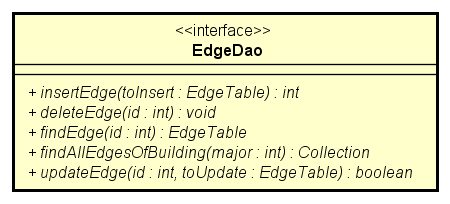
\includegraphics{img/EdgeDao.png}
        \caption{Interfaccia EdgeDao}\label{fig:model::dataaccess::dao::EdgeDao} 
    \end{figure}
    \begin{description}
\item[Nome:] \texttt{EdgeDao};
\item[Tipo:] Interfaccia;
\item[Visibilità:] \texttt{public};
\item[Utilizzo:] Viene utilizzata per rendere indipendenti l'invocazioni dei metodi per effettuare le operazioni CRUD sulla tabella "Edge" del database locale dalla loro implementazione;
\item[Descrizione:] Interfaccia che espone i metodi per un DAO per accedere alla tabella "Edge" del database locale;
\item[Metodi:] \
\begin{itemize}
\item \texttt{+ \textit{deleteEdge(id : int) : void}}\\
Metodo che permette la rimozione delle informazioni di un edificio dalla tabella "Edge" del database locale 
 \begin{description}
\item[Argomenti:] \
\begin{itemize}
\item \texttt{id : int}\\
Identificativo dell'arco di cui rimuovere le informazioni dal database locale\end{itemize}
\end{description}
\item \texttt{+ \textit{findAllEdgesOfBuilding(major : int) : Collection<EdgeTable>}}\\
Metodo che viene utilizzato per recuperare le informazioni di tutti gli archi presenti nella tabella "Edge" del database locale
 \begin{description}
\item[Argomenti:] \
\begin{itemize}
\item \texttt{major : int}\\
Identificativo major dell'edificio di cui si vogliono recuperare tutti gli archi\end{itemize}
\end{description}
\item \texttt{+ \textit{findEdge(id : int) : EdgeTable}}\\
Metodo per recuperare le informazioni di un arco dal database locale tramite il suo identificativo, sotto forma di oggetto EdgeTable
 \begin{description}
\item[Argomenti:] \
\begin{itemize}
\item \texttt{id : int}\\
Identificativo dell'arco di cui recuperare le informazioni\end{itemize}
\end{description}
\item \texttt{+ \textit{insertEdge(toInsert : EdgeTable) : int}}\\
Metodo che permette l'inserimento delle informazioni di un edificio in una entry della tabella "Edge" del database locale
 \begin{description}
\item[Argomenti:] \
\begin{itemize}
\item \texttt{toInsert : EdgeTable}\\
Oggetto di tipo EdgeTable che contiene le informazioni dell'arco\end{itemize}
\end{description}
\item \texttt{+ \textit{updateEdge(id : int, toUpdate : EdgeTable) : boolean}}\\
Metodo per aggiornare le informazioni di un edificio nella tabella "Edge" del database locale
 \begin{description}
\item[Argomenti:] \
\begin{itemize}
\item \texttt{id : int}\\
Identificativo dell'arco di cui aggiornare le informazioni\item \texttt{toUpdate : EdgeTable}\\
Oggetto che contiene le informazioni aggiornate dell'arco\end{itemize}
\end{description}
\end{itemize}
\end{description}

\subsubsection{model::dataaccess::dao::EdgeTable}

    \begin{figure}[H]
        \centering
        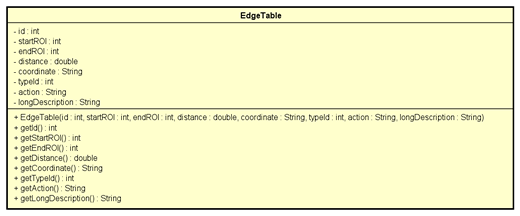
\includegraphics{img/EdgeTable.png}
        \caption{Classe EdgeTable}\label{fig:model::dataaccess::dao::EdgeTable} 
    \end{figure}
    \begin{description}
\item[Nome:] \texttt{EdgeTable};
\item[Tipo:] Classe;
\item[Visibilità:] \texttt{public};
\item[Utilizzo:] Viene utilizzata per recuperare le informazioni di una ennupla della tabella Edge del database locale ;
\item[Descrizione:] Classe che rappresenta una ennupla della tabella Edge del database locale;
\item[Attributi:] \
\begin{itemize}
\item \texttt{- action : String}\\
Descrizione dell'azione da compiere per arrivare dallo startROI all'endROI

\item \texttt{- coordinate : String}\\
Angolo rispetto al Nord polare presente lo startROI e l'endROI

\item \texttt{- distance : double}\\
Distanza tra lo startROI e l'endROI

\item \texttt{- endROI : int}\\
Nodo d'arrivo dell'arco

\item \texttt{- id : int}\\
Identificativo dell'Edge

\item \texttt{- longDescription : String}\\
Descrizione testuale estesa per raggiungere l'endROI a partire dallo startROI

\item \texttt{- startROI : int}\\
Nodo di partenza dell'arco

\item \texttt{- typeId : int}\\
Identificativo del tipo di Edge

\end{itemize}
\item[Metodi:] \
\begin{itemize}
\item \texttt{+ EdgeTable(id : int, startROI : int, endROI : int, distance : double, coordinate : String, typeId : int, action : String, longDescription : String)}\\
Costruttore della classe EdgeTable
 \begin{description}
\item[Argomenti:] \
\begin{itemize}
\item \texttt{id : int}\\
Identificativo dell'Edge\item \texttt{startROI : int}\\
Nodo di partenza dell'arco\item \texttt{endROI : int}\\
Nodo d'arrivo dell'arco\item \texttt{distance : double}\\
Distanza tra lo startROI e l'endROI\item \texttt{coordinate : String}\\
Angolo rispetto al Nord polare presente lo startROI e l'endROI\item \texttt{typeId : int}\\
Identificativo del tipo di Edge\item \texttt{action : String}\\
Descrizione dell'azione da compiere per arrivare dallo startROI all'endROI\item \texttt{longDescription : String}\\
Descrizione testuale estesa per raggiungere l'endROI a partire dallo startROI\end{itemize}
\end{description}
\item \texttt{+ getAction() : String}\\
Metodo che ritorna la descrizione dell'azione da compiere per arrivare dallo startROI all'endROI
 \item \texttt{+ getCoordinate() : String}\\
Metodo che ritorna l'angolo rispetto al Nord polare presente lo startROI e l'endROI
 \item \texttt{+ getDistance() : double}\\
Metodo che ritorna la distanza tra lo startROI e l'endROI
 \item \texttt{+ getEndROI() : int}\\
Metodo che ritorna il nodo d'arrivo dell'arco
 \item \texttt{+ getId() : int}\\
Metodo che ritorna l'identificativo dell'Edge
 \item \texttt{+ getLongDescription() : String}\\
Metodo che ritorna la descrizione testuale estesa per raggiungere l'endROI a partire dallo startROI
 \item \texttt{+ getStartROI() : int}\\
Metodo che ritorna il nodo di partenza dell'arco
 \item \texttt{+ getTypeId() : int}\\
Metodo che ritorna l'identificativo del tipo di Edge
 \end{itemize}
\end{description}

\subsubsection{model::dataaccess::dao::EdgeTypeContract}

    \begin{figure}[H]
        \centering
        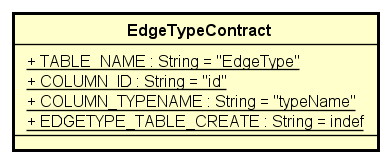
\includegraphics{img/EdgeTypeContract.png}
        \caption{Classe EdgeTypeContract}\label{fig:model::dataaccess::dao::EdgeTypeContract} 
    \end{figure}
    \begin{description}
\item[Nome:] \texttt{EdgeTypeContract};
\item[Tipo:] Classe;
\item[Visibilità:] \texttt{public};
\item[Utilizzo:] Utilizzata per reperire le informazioni corrette della tabella EdgeType del database locale;
\item[Descrizione:] Classe che contiene le informazioni corrette della tabella EdgeType del database locale;
\item[Attributi:] \
\begin{itemize}
\item \texttt{+ \underline{COLUMN\_ID : String \{readOnly\}}}\\
Valore della colonna id. Valore di default "id"

\item \texttt{+ \underline{COLUMN\_TYPENAME : String \{readOnly\}}}\\
Valore della colonna typeName. Valore di default "typeName"

\item \texttt{+ \underline{EDGETYPE\_TABLE\_CREATE : String \{readOnly\}}}\\
Query per la creazione della tabella

\item \texttt{+ \underline{TABLE\_NAME : String \{readOnly\}}}\\
Nome della tabella. Valore di default "EdgeType"

\end{itemize}
\end{description}

\subsubsection{model::dataaccess::dao::EdgeTypeDao}

    \begin{figure}[H]
        \centering
        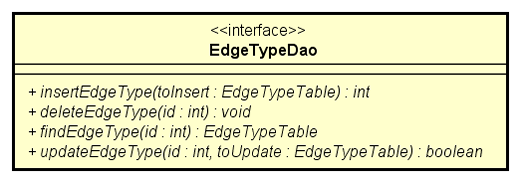
\includegraphics{img/EdgeTypeDao.png}
        \caption{Interfaccia EdgeTypeDao}\label{fig:model::dataaccess::dao::EdgeTypeDao} 
    \end{figure}
    \begin{description}
\item[Nome:] \texttt{EdgeTypeDao};
\item[Tipo:] Interfaccia;
\item[Visibilità:] \texttt{public};
\item[Utilizzo:] Viene utilizzata per rendere indipendenti l'invocazioni dei metodi per effettuare le operazioni CRUD sulla tabella "EdgeType" del database locale dalla loro implementazione;
\item[Descrizione:] Interfaccia che espone i metodi per un DAO per accedere alla tabella "EdgeType" del database locale;
\item[Metodi:] \
\begin{itemize}
\item \texttt{+ \textit{deleteEdgeType(id : int) : void}}\\
Metodo che permette la rimozione delle informazioni di un tipo di Edge dalla tabella "EdgeType" del database locale
 \begin{description}
\item[Argomenti:] \
\begin{itemize}
\item \texttt{id : int}\\
Identificativo del tipo di Edge di cui rimuovere le informazioni dal database locale\end{itemize}
\end{description}
\item \texttt{+ \textit{findEdgeType(id : int) : EdgeTypeTable}}\\
Metodo per recuperare le informazioni di un tipo di Edge dal database locale tramite il suo identificativo, sotto forma di oggetto EdgeTypeTable
 \begin{description}
\item[Argomenti:] \
\begin{itemize}
\item \texttt{id : int}\\
Identificativo del tipo di Edge di cui recuperare le informazioni\end{itemize}
\end{description}
\item \texttt{+ \textit{insertEdgeType(toInsert : EdgeTypeTable) : int}}\\
Metodo che permette l'inserimento delle informazioni del tipo di Edge in una entry della tabella "EdgeType" del database locale
 \begin{description}
\item[Argomenti:] \
\begin{itemize}
\item \texttt{toInsert : EdgeTypeTable}\\
Oggetto di tipo EdgeTypeTable che contiene le informazioni di un tipo di Edge\end{itemize}
\end{description}
\item \texttt{+ \textit{updateEdgeType(id : int, toUpdate : EdgeTypeTable) : boolean}}\\
Metodo per aggiornare le informazioni di un tipo di Edge nella tabella "EdgeType" del database locale
 \begin{description}
\item[Argomenti:] \
\begin{itemize}
\item \texttt{id : int}\\
Identificativo del tipo di Edge di cui aggiornare le informazioni\item \texttt{toUpdate : EdgeTypeTable}\\
Oggetto che contiene le informazioni aggiornate del tipo di Edge\end{itemize}
\end{description}
\end{itemize}
\end{description}

\subsubsection{model::dataaccess::dao::EdgeTypeTable}

    \begin{figure}[H]
        \centering
        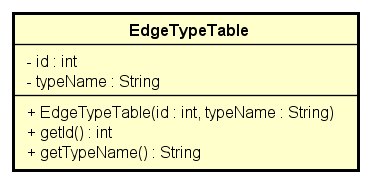
\includegraphics{img/EdgeTypeTable.png}
        \caption{Classe EdgeTypeTable}\label{fig:model::dataaccess::dao::EdgeTypeTable} 
    \end{figure}
    \begin{description}
\item[Nome:] \texttt{EdgeTypeTable};
\item[Tipo:] Classe;
\item[Visibilità:] \texttt{public};
\item[Utilizzo:] Viene utilizzata per recuperare le informazioni di una ennupla della tabella EdgeType del database locale ;
\item[Descrizione:] Classe che rappresenta una ennupla della tabella EdgeType del database locale;
\item[Attributi:] \
\begin{itemize}
\item \texttt{- id : int}\\
Identificativo numerico dell'oggetto EdgeTypeTable

\item \texttt{- typeName : String}\\
Identificativo numerico che permette di identificare il tipo di Edge

\end{itemize}
\item[Metodi:] \
\begin{itemize}
\item \texttt{+ EdgeTypeTable(id : int, typeName : String)}\\
Costruttore della classe EdgeTypeTable
 \begin{description}
\item[Argomenti:] \
\begin{itemize}
\item \texttt{id : int}\\
Identificativo numerico dell'oggetto EdgeTypeTable\item \texttt{typeName : String}\\
Identificativo numerico che permette di identificare il tipo di Edge\end{itemize}
\end{description}
\item \texttt{+ getId() : int}\\
Metodo che restituisce l'identificativo numerico dell'oggetto EdgeTypeTable
 \item \texttt{+ getTypeName() : String}\\
Metodo che restituisce l'identificativo numerico che permette di identificare il tipo di Edge
 \end{itemize}
\end{description}

\subsubsection{model::dataaccess::dao::MapsDbContract}

    \begin{figure}[H]
        \centering
        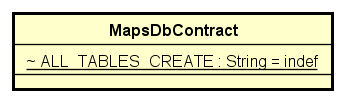
\includegraphics{img/MapsDbContract.png}
        \caption{Classe MapsDbContract}\label{fig:model::dataaccess::dao::MapsDbContract} 
    \end{figure}
    \begin{description}
\item[Nome:] \texttt{MapsDbContract};
\item[Tipo:] Classe;
\item[Visibilità:] \texttt{public};
\item[Utilizzo:] Viene utilizzata per reperire la query corretta per creare tutte le tabelle del database locale;
\item[Descrizione:] Classe che contiene la query corretta per creare tutte le tabelle del database locale;
\item[Attributi:] \
\begin{itemize}
\item \texttt{~ \underline{ALL\_TABLES\_CREATE : String \{readOnly\}}}\\
Query per la creazione di tutte le tabelle del database locale

\end{itemize}
\end{description}

\subsubsection{model::dataaccess::dao::MapsDbHelper}

    \begin{figure}[H]
        \centering
        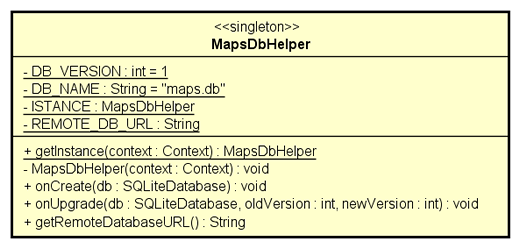
\includegraphics{img/MapsDbHelper.png}
        \caption{Classe MapsDbHelper}\label{fig:model::dataaccess::dao::MapsDbHelper} 
    \end{figure}
    \begin{description}
\item[Nome:] \texttt{MapsDbHelper};
\item[Tipo:] Classe;
\item[Componenti delle librerie utilizzate:] \
\begin{itemize}
\item \texttt{android.database.sqlite.SQLiteOpenHelper (Android)}.

\end{itemize}
\item[Visibilità:] \texttt{public};
\item[Utilizzo:] Viene utilizzata per ottenere un'istanza di SQLiteDatabase o l'URL del database remoto;
\item[Descrizione:] Classe che rappresenta un aiutante per ottenere informazioni su come accedere al database locale e remoto;
\item[Attributi:] \
\begin{itemize}
\item \texttt{- \underline{DB\_NAME : String \{readOnly\}}}\\
Nome del database locale. Valore di default: "maps.db"

\item \texttt{- \underline{DB\_VERSION : int \{readOnly\}}}\\
Numero di versione del database locale. Valore di default: "1"

\item \texttt{- \underline{ISTANCE : MapsDbHelper \{readOnly\}}}\\
Istanza di MapsDbHelper salvata per poter essere condivisa

\item \texttt{- \underline{REMOTE\_DB\_URL : String \{readOnly\}}}\\
URL del database remoto

\end{itemize}
\item[Metodi:] \
\begin{itemize}
\item \texttt{+ \underline{getInstance() : MapsDbHelper}}\\
Metodo che ritorna una istanza di MapsDbHelper
 \item \texttt{+ getRemoteDatabaseURL() : String}\\
Metodo che ritorna l'URL del database remoto
 \item \texttt{- MapsDbHelper()}\\
Costruttore della classe MapsDbHelper
 \item \texttt{+ onCreate(db : SQLiteDatabase) : void}\\
Metodo che viene chiamato la prima volta che viene creato il database
 \begin{description}
\item[Argomenti:] \
\begin{itemize}
\item \texttt{db : SQLiteDatabase}\\
Riferimento al database\end{itemize}
\end{description}
\item \texttt{+ onUpgrade(db : SQLiteDatabase, oldVersion : int, newVersione : int) : void}\\
Metodo che viene chiamato per effettuare l'upgrade del database
 \begin{description}
\item[Argomenti:] \
\begin{itemize}
\item \texttt{db : SQLiteDatabase}\\
Riferimento al database\item \texttt{oldVersion : int}\\
Numero di versione del vecchio database\item \texttt{newVersione : int}\\
Numero di versione del nuovo database\end{itemize}
\end{description}
\end{itemize}
\end{description}

\subsubsection{model::dataaccess::dao::PhotoContract}

    \begin{figure}[H]
        \centering
        \includegraphics{img/PhotoContract.png}
        \caption{Classe PhotoContract}\label{fig:model::dataaccess::dao::PhotoContract} 
    \end{figure}
    \begin{description}
\item[Nome:] \texttt{PhotoContract};
\item[Tipo:] Classe;
\item[Visibilità:] \texttt{public};
\item[Utilizzo:] Utilizzata per reperire le informazioni corrette della tabella Photo del database locale;
\item[Descrizione:] Classe che contiene le informazioni corrette della tabella Photo del database locale;
\item[Attributi:] \
\begin{itemize}
\item \texttt{+ \underline{COLUMN\_EDGEID : String \{readOnly\}}}\\
Valore della colonna edgeId. Valore di default "edgeId"

\item \texttt{+ \underline{COLUMN\_ID : String \{readOnly\}}}\\
Valore della colonna id. Valore di default "id"

\item \texttt{+ \underline{COLUMN\_URL : String \{readOnly\}}}\\
Valore della colonna url. Valore di default "url"

\item \texttt{+ \underline{PHOTO\_TABLE\_CREATE : String \{readOnly\}}}\\
Query per la creazione della tabella

\item \texttt{+ \underline{TABLE\_NAME : String \{readOnly\}}}\\
Nome della tabella.Valore di default "Photo"

\end{itemize}
\end{description}

\subsubsection{model::dataaccess::dao::PhotoDao}

    \begin{figure}[H]
        \centering
        \includegraphics{img/PhotoDao.png}
        \caption{Interfaccia PhotoDao}\label{fig:model::dataaccess::dao::PhotoDao} 
    \end{figure}
    \begin{description}
\item[Nome:] \texttt{PhotoDao};
\item[Tipo:] Interfaccia;
\item[Visibilità:] \texttt{public};
\item[Utilizzo:] Viene utilizzata per rendere indipendenti l'invocazioni dei metodi per effettuare le operazioni CRUD sulla tabella "Photo" del database locale dalla loro implementazione;
\item[Descrizione:] Interfaccia che espone i metodi per un DAO per accedere alla tabella "Photo" del database locale;
\item[Metodi:] \
\begin{itemize}
\item \texttt{+ \textit{deletePhoto(id : int) : void}}\\
Metodo che permette la rimozione delle informazioni di una foto dalla tabella "Photo" del database locale
 \begin{description}
\item[Argomenti:] \
\begin{itemize}
\item \texttt{id : int}\\
Identificativo della foto di cui rimuovere le informazioni dal database locale\end{itemize}
\end{description}
\item \texttt{+ \textit{findAllPhotosOfEdge(id : int) : Collection<PhotoTable>}}\\
Metodo che viene utilizzato per recuperare le informazioni di tutte foto associate ad un Edge presenti nella tabella "Photo" del database locale
 \begin{description}
\item[Argomenti:] \
\begin{itemize}
\item \texttt{id : int}\\
Identificativo dell'Edge\end{itemize}
\end{description}
\item \texttt{+ \textit{findPhoto(id : int) : PhotoTable}}\\
Metodo per recuperare le informazioni di una foto dal database locale tramite il suo identificativo, sotto forma di oggetto PhotoTable
 \begin{description}
\item[Argomenti:] \
\begin{itemize}
\item \texttt{id : int}\\
Identificativo della foto\end{itemize}
\end{description}
\item \texttt{+ \textit{insertPhoto(toInser : PhotoTable) : int}}\\
Metodo che permette l'inserimento delle informazioni di una foto in una entry della tabella "Photo" del database locale
 \begin{description}
\item[Argomenti:] \
\begin{itemize}
\item \texttt{toInser : PhotoTable}\\
Oggetto di tipo Photo che contiene le informazioni della foto\end{itemize}
\end{description}
\item \texttt{+ \textit{updatePhoto(id : int, toUpdate : PhotoTable) : boolean}}\\
Metodo per aggiornare le informazioni di una foto nella tabella "Photo" del database locale
 \begin{description}
\item[Argomenti:] \
\begin{itemize}
\item \texttt{id : int}\\
Identificativo della foto di cui aggiornare le informazioni\item \texttt{toUpdate : PhotoTable}\\
Oggetto che contiene le informazioni aggiornate della foto\end{itemize}
\end{description}
\end{itemize}
\end{description}

\subsubsection{model::dataaccess::dao::PhotoTable}

    \begin{figure}[H]
        \centering
        \includegraphics{img/PhotoTable.png}
        \caption{Classe PhotoTable}\label{fig:model::dataaccess::dao::PhotoTable} 
    \end{figure}
    \begin{description}
\item[Nome:] \texttt{PhotoTable};
\item[Tipo:] Classe;
\item[Visibilità:] \texttt{public};
\item[Utilizzo:] Viene utilizzata per recuperare le informazioni di una ennupla della tabella Photo del database locale ;
\item[Descrizione:] Classe che rappresenta una ennupla della tabella Photo del database locale;
\item[Attributi:] \
\begin{itemize}
\item \texttt{- edgeId : int}\\
Identificativo numerico dell'Edge a cui fa riferimento la foto

\item \texttt{- id : int}\\
Identificativo numerico dell'oggetto PhotoTable

\item \texttt{- url : String}\\
Stringa che rappresenta l'URL dove si può reperire la foto

\end{itemize}
\item[Metodi:] \
\begin{itemize}
\item \texttt{+ getEdgeId() : int}\\
Metodo che viene utilizzato per recuperare l'identificativo numerico dell'Edge a cui fa riferimento la foto
 \item \texttt{+ getId() : int}\\
Metodo che viene utilizzato per recuperare l'identificativo numerico della foto nel database
 \item \texttt{+ getUrl() : String}\\
Metodo per recuperare la stringa che rappresenta l'URL dove è possibile reperire la foto 
 \item \texttt{+ PhotoTable(id : int, url : String, edgeId : int)}\\
Costruttore della classe PhotoTable
 \begin{description}
\item[Argomenti:] \
\begin{itemize}
\item \texttt{id : int}\\
Identificativo numerico della foto nel database locale\item \texttt{url : String}\\
Stringa che rappresenta l'URL dove si può reperire la foto\item \texttt{edgeId : int}\\
Identificativo numerico dell'Edge a cui fa riferimento la foto\end{itemize}
\end{description}
\end{itemize}
\end{description}

\subsubsection{model::dataaccess::dao::PointOfInterestContract}

    \begin{figure}[H]
        \centering
        \includegraphics{img/PointOfInterestContract.png}
        \caption{Classe PointOfInterestContract}\label{fig:model::dataaccess::dao::PointOfInterestContract} 
    \end{figure}
    \begin{description}
\item[Nome:] \texttt{PointOfInterestContract};
\item[Tipo:] Classe;
\item[Visibilità:] \texttt{public};
\item[Utilizzo:] Utilizzata per reperire le informazioni corrette della tabella POI del database locale;
\item[Descrizione:] Classe che contiene le informazioni corrette della tabella POI del database locale;
\item[Attributi:] \
\begin{itemize}
\item \texttt{+ \underline{COLUMN\_CATEGORYID : String \{readOnly\}}}\\
Valore della colonna categoryId. Valore di default "categoryId"

\item \texttt{+ \underline{COLUMN\_DESCRIPTION : String \{readOnly\}}}\\
Valore della colonna description. Valore di default "description"

\item \texttt{+ \underline{COLUMN\_ID : String \{readOnly\}}}\\
Valore della colonna id. Valore di default "id"

\item \texttt{+ \underline{COLUMN\_NAME : String \{readOnly\}}}\\
Valore della colonna name. Valore di default "name"

\item \texttt{+ \underline{POI\_TABLE\_CREATE : String \{readOnly\}}}\\
Contiene la query di creazione della tabella

\item \texttt{+ \underline{TABLE\_NAME : String \{readOnly\}}}\\
Nome della tabella.Valore di default "POI"

\end{itemize}
\end{description}

\subsubsection{model::dataaccess::dao::PointOfInterestDao}

    \begin{figure}[H]
        \centering
        \includegraphics{img/PointOfInterestDao.png}
        \caption{Interfaccia PointOfInterestDao}\label{fig:model::dataaccess::dao::PointOfInterestDao} 
    \end{figure}
    \begin{description}
\item[Nome:] \texttt{PointOfInterestDao};
\item[Tipo:] Interfaccia;
\item[Visibilità:] \texttt{public};
\item[Utilizzo:] Viene utilizzata per rendere indipendenti l'invocazioni dei metodi per effettuare le operazioni CRUD sulla tabella "POI" del database locale dalla loro implementazione;
\item[Descrizione:] Interfaccia che espone i metodi per un DAO per accedere alla tabella "POI" del database locale;
\item[Metodi:] \
\begin{itemize}
\item \texttt{+ \textit{deletePointOfInterest(id : int) : void}}\\
Metodo che permette la rimozione delle informazioni di un edificio dalla tabella "POI" del database locale 
 \begin{description}
\item[Argomenti:] \
\begin{itemize}
\item \texttt{id : int}\\
Identificativo del POI di cui rimuovere le informazioni dal database locale\end{itemize}
\end{description}
\item \texttt{+ \textit{findAllPointsWithMajor(major : int) : Collection<PointOfInterestTable>}}\\
Metodo che viene utilizzato per recuperare le informazioni di tutti gli edifici presenti nella tabella "POI" del database locale
 \begin{description}
\item[Argomenti:] \
\begin{itemize}
\item \texttt{major : int}\\
Identificativo Major associato a tutti i beacon presenti in uno stesso edificio\end{itemize}
\end{description}
\item \texttt{+ \textit{findPointOfInterest(id : int) : PointOfInterestTable}}\\
Metodo per recuperare le informazioni di un edificio dal database locale tramite il suo identificativo, sotto forma di oggetto PointOfInterestTable
 \begin{description}
\item[Argomenti:] \
\begin{itemize}
\item \texttt{id : int}\\
Identificativo del POI di cui recuperare le informazioni\end{itemize}
\end{description}
\item \texttt{+ \textit{insertPointOfInterest(toInsert : PointOfInterestTable) : int}}\\
Metodo che permette l'inserimento delle informazioni di un edificio in una entry della tabella "POI" del database locale
 \begin{description}
\item[Argomenti:] \
\begin{itemize}
\item \texttt{toInsert : PointOfInterestTable}\\
Oggetto di tipo PointOfInterestTable che contiene le informazioni dell'edificio\end{itemize}
\end{description}
\item \texttt{+ \textit{updatePointOfInterest(id : int, toUpdate : PointOfInterestTable) : boolean}}\\
Metodo per aggiornare le informazioni di un edificio nella tabella "POI" del database locale
 \begin{description}
\item[Argomenti:] \
\begin{itemize}
\item \texttt{id : int}\\
Identificativo del POI di cui aggiornare le informazioni\item \texttt{toUpdate : PointOfInterestTable}\\
Oggetto che contiene le informazioni aggiornate del POI\end{itemize}
\end{description}
\end{itemize}
\end{description}

\subsubsection{model::dataaccess::dao::PointOfInterestTable}

    \begin{figure}[H]
        \centering
        \includegraphics{img/PointOfInterestTable.png}
        \caption{Classe PointOfInterestTable}\label{fig:model::dataaccess::dao::PointOfInterestTable} 
    \end{figure}
    \begin{description}
\item[Nome:] \texttt{PointOfInterestTable};
\item[Tipo:] Classe;
\item[Visibilità:] \texttt{public};
\item[Utilizzo:] Viene utilizzata per recuperare le informazioni di una ennupla della tabella PointOfInterest del database locale ;
\item[Descrizione:] Classe che rappresenta una ennupla della tabella PointOfInterest del database locale;
\item[Attributi:] \
\begin{itemize}
\item \texttt{- categoryId : int}\\
Identificativo della categoria a cui appartiene il POI

\item \texttt{- description : String}\\
Descrizione del POI

\item \texttt{- id : int}\\
Identificativo del POI

\item \texttt{- name : String}\\
Nome del POI

\end{itemize}
\item[Metodi:] \
\begin{itemize}
\item \texttt{+ getCategoryId() : int}\\
Metodo che ritorna l'identificativo del POI
 \item \texttt{+ getDescription() : String}\\
Metodo che ritorna la descrizione del POI
 \item \texttt{+ getId() : int}\\
Metodo che ritorna l'identificativo del POI
 \item \texttt{+ getName() : String}\\
Metodo che ritorna il nome dell'edificio
 \item \texttt{+ PointOfInterestTable(description : String, id : int, name : String, category : int)}\\
Costruttore della classe PointOfInterestTable
 \begin{description}
\item[Argomenti:] \
\begin{itemize}
\item \texttt{description : String}\\
Descrizione del POI\item \texttt{id : int}\\
Identificativo del POI\item \texttt{name : String}\\
Nome del POI\item \texttt{category : int}\\
Identificativo della categoria a cui appartiene il POI\end{itemize}
\end{description}
\end{itemize}
\end{description}

\subsubsection{model::dataaccess::dao::RegionOfInterestContract}

    \begin{figure}[H]
        \centering
        \includegraphics{img/RegionOfInterestContract.png}
        \caption{Classe RegionOfInterestContract}\label{fig:model::dataaccess::dao::RegionOfInterestContract} 
    \end{figure}
    \begin{description}
\item[Nome:] \texttt{RegionOfInterestContract};
\item[Tipo:] Classe;
\item[Visibilità:] \texttt{public};
\item[Utilizzo:] Utilizzata per reperire le informazioni corrette della tabella ROI del database locale;
\item[Descrizione:] Classe che contiene le informazioni corrette della tabella ROI del database locale;
\item[Attributi:] \
\begin{itemize}
\item \texttt{+ \underline{COLUMN\_ID : String \{readOnly\}}}\\
Valore della colonna id. Valore di default "id"

\item \texttt{+ \underline{COLUMN\_MAJOR : String \{readOnly\}}}\\
Valore della colonna major. Valore di default "major"

\item \texttt{+ \underline{COLUMN\_MINOR : String \{readOnly\}}}\\
Valore della colonna minor. Valore di default "minor"

\item \texttt{+ \underline{COLUMN\_UUID : String \{readOnly\}}}\\
Valore della colonna uuid. Valore di default "uuid"

\item \texttt{+ \underline{ROI\_TABLE\_CREATE : String \{readOnly\}}}\\
Contiene la query di creazione della tabella

\item \texttt{+ \underline{TABLE\_NAME : String \{readOnly\}}}\\
Nome della tabella. Valore di default "ROI"

\end{itemize}
\end{description}

\subsubsection{model::dataaccess::dao::RegionOfInterestDao}

    \begin{figure}[H]
        \centering
        \includegraphics{img/RegionOfInterestDao.png}
        \caption{Interfaccia RegionOfInterestDao}\label{fig:model::dataaccess::dao::RegionOfInterestDao} 
    \end{figure}
    \begin{description}
\item[Nome:] \texttt{RegionOfInterestDao};
\item[Tipo:] Interfaccia;
\item[Visibilità:] \texttt{public};
\item[Utilizzo:] Viene utilizzata per rendere indipendenti l'invocazioni dei metodi per effettuare le operazioni CRUD sulla tabella "ROI" del database locale dalla loro implementazione;
\item[Descrizione:] Interfaccia che espone i metodi per un DAO per accedere alla tabella "ROI" del database locale;
\item[Metodi:] \
\begin{itemize}
\item \texttt{+ \textit{deleteRegionOfInterest(id : int) : void}}\\
Metodo che permette la rimozione delle informazioni di una RegionOfInterest dalla tabella "ROI" del database locale
 \begin{description}
\item[Argomenti:] \
\begin{itemize}
\item \texttt{id : int}\\
Identificativo della RegionOfInterest di cui rimuovere le informazioni dal database locale\end{itemize}
\end{description}
\item \texttt{+ \textit{findAllRegionsWithMajor(major : int) : Collection<RegionOfInterestTable>}}\\
Metodo che viene utilizzato per recuperare le informazioni di tutte le RegionOfInterest associato ad certo edificio, dato il major dell'edificio
 \begin{description}
\item[Argomenti:] \
\begin{itemize}
\item \texttt{major : int}\\
Major dell'edificio\end{itemize}
\end{description}
\item \texttt{+ \textit{findRegionOfInterest(id : int) : RegionOfInterestTable}}\\
Metodo per recuperare le informazioni di una RegionOfInterest dal database locale tramite il suo identificativo, sotto forma di oggetto RegionOfInterestTable
 \begin{description}
\item[Argomenti:] \
\begin{itemize}
\item \texttt{id : int}\\
Identificativo della RegionOfInterest di cui recuperare le informazioni\end{itemize}
\end{description}
\item \texttt{+ \textit{insertRegionOfInterest(toInsert : RegionOfInterestTable) : int}}\\
Metodo che permette l'inserimento delle informazioni di una RegionOfInterest in una entry della tabella "ROI" del database locale
 \begin{description}
\item[Argomenti:] \
\begin{itemize}
\item \texttt{toInsert : RegionOfInterestTable}\\
Oggetto di tipo RegionOfInterestTable che contiene le informazioni della RegionOfInterest\end{itemize}
\end{description}
\item \texttt{+ \textit{updateRegionOfInterest(id : int, toUpdate : RegionOfInterestTable) : boolean}}\\
Metodo per aggiornare le informazioni di una RegionOfInterest nella tabella "ROI" del database locale
 \begin{description}
\item[Argomenti:] \
\begin{itemize}
\item \texttt{id : int}\\
Identificativo della RegionOfInterest di cui aggiornare le informazioni\item \texttt{toUpdate : RegionOfInterestTable}\\
Oggetto che contiene le informazioni aggiornate della RegionOfInterest\end{itemize}
\end{description}
\end{itemize}
\end{description}

\subsubsection{model::dataaccess::dao::RegionOfInterestTable}

    \begin{figure}[H]
        \centering
        \includegraphics{img/RegionOfInterestTable.png}
        \caption{Classe RegionOfInterestTable}\label{fig:model::dataaccess::dao::RegionOfInterestTable} 
    \end{figure}
    \begin{description}
\item[Nome:] \texttt{RegionOfInterestTable};
\item[Tipo:] Classe;
\item[Visibilità:] \texttt{public};
\item[Utilizzo:] Viene utilizzata per recuperare le informazioni di una ennupla della tabella RegionOfInterest del database locale ;
\item[Descrizione:] Classe che rappresenta una ennupla della tabella RegionOfInterest del database locale;
\item[Attributi:] \
\begin{itemize}
\item \texttt{- id : int}\\
Identificativo della RegionOfInterest

\item \texttt{- major : int}\\
Major dell'edificio

\item \texttt{- minor : int}\\
Identificativo del beacon associato alla ROI

\item \texttt{- uuid : String}\\
UUID dell'applicazione

\end{itemize}
\item[Metodi:] \
\begin{itemize}
\item \texttt{+ getId() : int}\\
Metodo che ritorna l'identificativo della ROI
 \item \texttt{+ getMajor() : int}\\
Metodo che ritorna il major dell'edificio
 \item \texttt{+ getMinor() : int}\\
Metodo che ritorna l'identificativo del beacon associato alla ROI
 \item \texttt{+ getUUID() : String}\\
Metodo che ritorna l'UUID dell'applicazione
 \item \texttt{+ RegionOfInterestTable(id : int, uuid : String, major : int, minor : int)}\\
Costruttore della classe RegionOfInterestTable
 \begin{description}
\item[Argomenti:] \
\begin{itemize}
\item \texttt{id : int}\\
Identificativo della RegionOfInterest\item \texttt{uuid : String}\\
Identificativo dell'applicazione\item \texttt{major : int}\\
Major dell'edificio\item \texttt{minor : int}\\
Identificativo del beacon associato alla ROI\end{itemize}
\end{description}
\end{itemize}
\end{description}

\subsubsection{model::dataaccess::dao::RemoteBuildingDao}

    \begin{figure}[H]
        \centering
        \includegraphics{img/RemoteBuildingDao.png}
        \caption{Classe RemoteBuildingDao}\label{fig:model::dataaccess::dao::RemoteBuildingDao} 
    \end{figure}
    \begin{description}
\item[Nome:] \texttt{RemoteBuildingDao};
\item[Tipo:] Classe;
\item[Componenti delle librerie utilizzate:] \
\begin{itemize}
\item \texttt{com.google.api.client.json.JsonObjectParser
};

\item \texttt{com.google.gson.JsonArray};

\item \texttt{com.google.gson.JsonElement};

\item \texttt{com.google.gson.JsonObject}.

\end{itemize}
\item[Visibilità:] \texttt{public};
\item[Utilizzo:] È utilizzata per la conversione di oggetti JSON in oggetti persistenti BuildingTable che rappresentano la tabella "Building" del database locale;
\item[Descrizione:] Classe di utility per la conversione da JSON a BuildingTable;
\item[Metodi:] \
\begin{itemize}
\item \texttt{+ fromJSONToTable(object : JsonObject) : BuildingTable}\\
Metodo utilizzato per la conversione di un oggetto JsonObject in un oggetto BuildingTable, che viene ritornato
 \begin{description}
\item[Argomenti:] \
\begin{itemize}
\item \texttt{object : JsonObject}\\
Oggetto JSON che rappresenta un oggetto di tipo BuildingTable\end{itemize}
\end{description}
\item \texttt{+ RemoteBuildingDao()}\\
Costruttore di default per la classe RemoteBuildingDao
 \end{itemize}
\end{description}

\subsubsection{model::dataaccess::dao::RemoteCategoryDao}

    \begin{figure}[H]
        \centering
        \includegraphics{img/RemoteCategoryDao.png}
        \caption{Classe RemoteCategoryDao}\label{fig:model::dataaccess::dao::RemoteCategoryDao} 
    \end{figure}
    \begin{description}
\item[Nome:] \texttt{RemoteCategoryDao};
\item[Tipo:] Classe;
\item[Componenti delle librerie utilizzate:] \
\begin{itemize}
\item \texttt{com.google.api.client.json.JsonObjectParser
};

\item \texttt{com.google.gson.JsonArray};

\item \texttt{com.google.gson.JsonElement};

\item \texttt{com.google.gson.JsonObject}.

\end{itemize}
\item[Visibilità:] \texttt{public};
\item[Utilizzo:] È utilizzata per la conversione di oggetti JSON in oggetti persistenti CategoryTable che rappresentano la tabella "Category" del database locale;
\item[Descrizione:] Classe di utility per la conversione da JSON a CategoryTable;
\item[Metodi:] \
\begin{itemize}
\item \texttt{+ fromJSONToTable(object : JsonObject) : CategoryTable}\\
Metodo utilizzato per la conversione di un oggetto JsonObject in un oggetto CategoryTable, che viene ritornato
 \begin{description}
\item[Argomenti:] \
\begin{itemize}
\item \texttt{object : JsonObject}\\
Oggetto JSON che rappresenta un oggetto di tipo CategoryTable\end{itemize}
\end{description}
\item \texttt{+ RemoteCategoryDao()}\\
Costruttore di default per la classe RemoteCategoryDao
 \end{itemize}
\end{description}

\subsubsection{model::dataaccess::dao::RemoteDaoFactory}

    \begin{figure}[H]
        \centering
        \includegraphics{img/RemoteDaoFactory.png}
        \caption{Classe RemoteDaoFactory}\label{fig:model::dataaccess::dao::RemoteDaoFactory} 
    \end{figure}
    \begin{description}
\item[Nome:] \texttt{RemoteDaoFactory};
\item[Tipo:] Classe;
\item[Visibilità:] \texttt{public};
\item[Utilizzo:] Viene utilizzata per creare e ottenere oggetti DAO remoti;
\item[Descrizione:] Classe che rappresenta la factory per creare tutti gli oggetti DAO remoti;
\item[Metodi:] \
\begin{itemize}
\item \texttt{+ getBuildingDao() : RemoteBuildingDao}\\
Metodo che viene utilizzato per ottenere un'istanza di RemoteBuildingDao
 \item \texttt{+ getCategoryDao() : RemoteCategoryDao}\\
Metodo che viene utilizzato per ottenere un'istanza di RemoteCategoryDao
 \item \texttt{+ getEdgeDao() : RemoteEdgeDao}\\
Metodo che viene utilizzato per ottenere un'istanza di RemoteEdgeDao
 \item \texttt{+ getEdgeTypeDao() : RemoteEdgeTypeDao}\\
Metodo che viene utilizzato per ottenere un'istanza di RemoteEdgeTypeDao
 \item \texttt{+ getPhotoDao() : RemotePhotoDao}\\
Metodo che viene utilizzato per ottenere un'istanza di RemotePhotoDao
 \item \texttt{+ getPointOfInterestDao() : RemotePointOfInterestDao}\\
Metodo che viene utilizzato per ottenere un'istanza di RemotePointOfInterestDao
 \item \texttt{+ getRegionOfInterestDao() : RemoteRegionOfInterestDao}\\
Metodo che viene utilizzato per ottenere un'istanza di RemoteRegionOfInterestDao
 \item \texttt{+ getRoiPoiDao() : RemoteRoiPoiDao}\\
Metodo che viene utilizzato per ottenere un'istanza di RemoteRoiPoiDao
 \item \texttt{+ RemoteDaoFactory()}\\
Costruttore di default per la classe RemoteDaoFactory
 \end{itemize}
\end{description}

\subsubsection{model::dataaccess::dao::RemoteEdgeDao}

    \begin{figure}[H]
        \centering
        \includegraphics{img/RemoteEdgeDao.png}
        \caption{Classe RemoteEdgeDao}\label{fig:model::dataaccess::dao::RemoteEdgeDao} 
    \end{figure}
    \begin{description}
\item[Nome:] \texttt{RemoteEdgeDao};
\item[Tipo:] Classe;
\item[Componenti delle librerie utilizzate:] \
\begin{itemize}
\item \texttt{com.google.api.client.json.JsonObjectParser
};

\item \texttt{com.google.gson.JsonArray};

\item \texttt{com.google.gson.JsonElement};

\item \texttt{com.google.gson.JsonObject}.

\end{itemize}
\item[Visibilità:] \texttt{public};
\item[Utilizzo:] È utilizzata per la conversione di oggetti JSON in oggetti persistenti EdgeTable che rappresentano la tabella "Edge" del database locale;
\item[Descrizione:] Classe di utility per la conversione da JSON a EdgeTable;
\item[Metodi:] \
\begin{itemize}
\item \texttt{+ fromJSONToTable(object : JsonObject) : EdgeTable}\\
Metodo utilizzato per la conversione di un oggetto JsonObject in un oggetto EdgeTable, che viene ritornato
 \begin{description}
\item[Argomenti:] \
\begin{itemize}
\item \texttt{object : JsonObject}\\
Oggetto JSON che rappresenta un oggetto di tipo EdgeTable\end{itemize}
\end{description}
\item \texttt{+ RemoteEdgeDao()}\\
Costruttore di default per la classe RemoteEdgeDao
 \end{itemize}
\end{description}

\subsubsection{model::dataaccess::dao::RemoteEdgeTypeDao}

    \begin{figure}[H]
        \centering
        \includegraphics{img/RemoteEdgeTypeDao.png}
        \caption{Classe RemoteEdgeTypeDao}\label{fig:model::dataaccess::dao::RemoteEdgeTypeDao} 
    \end{figure}
    \begin{description}
\item[Nome:] \texttt{RemoteEdgeTypeDao};
\item[Tipo:] Classe;
\item[Componenti delle librerie utilizzate:] \
\begin{itemize}
\item \texttt{com.google.api.client.json.JsonObjectParser
};

\item \texttt{com.google.gson.JsonArray};

\item \texttt{com.google.gson.JsonElement};

\item \texttt{com.google.gson.JsonObject}.

\end{itemize}
\item[Visibilità:] \texttt{public};
\item[Utilizzo:] È utilizzata per la conversione di oggetti JSON in oggetti persistenti EdgeTypeTable che rappresentano la tabella "EdgeType" del database locale;
\item[Descrizione:] Classe di utility per la conversione da JSON a EdgeTypeTable;
\item[Metodi:] \
\begin{itemize}
\item \texttt{+ fromJSONToTable(object : JsonObject) : EdgeTypeTable}\\
Metodo utilizzato per la conversione di un oggetto JsonObject in un oggetto EdgeTypeTable, che viene ritornato
 \begin{description}
\item[Argomenti:] \
\begin{itemize}
\item \texttt{object : JsonObject}\\
Oggetto JSON che rappresenta un oggetto di tipo EdgeTypeTable\end{itemize}
\end{description}
\item \texttt{+ RemoteEdgeTypeDao()}\\
Costruttore di default per la classe RemoteEdgeTypeDao
 \end{itemize}
\end{description}

\subsubsection{model::dataaccess::dao::RemotePhotoDao}

    \begin{figure}[H]
        \centering
        \includegraphics{img/RemotePhotoDao.png}
        \caption{Classe RemotePhotoDao}\label{fig:model::dataaccess::dao::RemotePhotoDao} 
    \end{figure}
    \begin{description}
\item[Nome:] \texttt{RemotePhotoDao};
\item[Tipo:] Classe;
\item[Componenti delle librerie utilizzate:] \
\begin{itemize}
\item \texttt{com.google.api.client.json.JsonObjectParser
};

\item \texttt{com.google.gson.JsonArray};

\item \texttt{com.google.gson.JsonElement};

\item \texttt{com.google.gson.JsonObject}.

\end{itemize}
\item[Visibilità:] \texttt{public};
\item[Utilizzo:] È utilizzata per la conversione di oggetti JSON in oggetti persistenti PhotoTable che rappresentano la tabella "Photo" del database locale;
\item[Descrizione:] Classe di utility per la conversione da JSON a PhotoTable;
\item[Metodi:] \
\begin{itemize}
\item \texttt{+ fromJSONToTable(object : JsonObject) : PhotoTable}\\
Metodo utilizzato per la conversione di un oggetto JsonObject in un oggetto PhotoTable, che viene ritornato
 \begin{description}
\item[Argomenti:] \
\begin{itemize}
\item \texttt{object : JsonObject}\\
Oggetto JSON che rappresenta un oggetto di tipo PhotoTable\end{itemize}
\end{description}
\item \texttt{+ RemotePhotoDao()}\\
Costruttore di default per la classe RemotePhotoDao
 \end{itemize}
\end{description}

\subsubsection{model::dataaccess::dao::RemotePointOfInterestDao}

    \begin{figure}[H]
        \centering
        \includegraphics{img/RemotePointOfInterestDao.png}
        \caption{Classe RemotePointOfInterestDao}\label{fig:model::dataaccess::dao::RemotePointOfInterestDao} 
    \end{figure}
    \begin{description}
\item[Nome:] \texttt{RemotePointOfInterestDao};
\item[Tipo:] Classe;
\item[Componenti delle librerie utilizzate:] \
\begin{itemize}
\item \texttt{com.google.api.client.json.JsonObjectParser
};

\item \texttt{com.google.gson.JsonArray};

\item \texttt{com.google.gson.JsonElement};

\item \texttt{com.google.gson.JsonObject}.

\end{itemize}
\item[Visibilità:] \texttt{public};
\item[Utilizzo:] È utilizzata per la conversione di oggetti JSON in oggetti persistenti PointOfInterestTable che rappresentano la tabella "POI" del database locale;
\item[Descrizione:] Classe di utility per la conversione da JSON a PointOfInterestTable;
\item[Metodi:] \
\begin{itemize}
\item \texttt{+ fromJSONToTable(object : JsonObject) : PointOfInterestTable}\\
Metodo utilizzato per la conversione di un oggetto JsonObject in un oggetto PointOfInterestTable, che viene ritornato
 \begin{description}
\item[Argomenti:] \
\begin{itemize}
\item \texttt{object : JsonObject}\\
Oggetto JSON che rappresenta un oggetto di tipo PointOfInterestTable\end{itemize}
\end{description}
\item \texttt{+ RemotePointOfInterestDao()}\\
Costruttore di default per la classe RemotePointOfInterestDao
 \end{itemize}
\end{description}

\subsubsection{model::dataaccess::dao::RemoteRegionOfInterestDao}

    \begin{figure}[H]
        \centering
        \includegraphics{img/RemoteRegionOfInterestDao.png}
        \caption{Classe RemoteRegionOfInterestDao}\label{fig:model::dataaccess::dao::RemoteRegionOfInterestDao} 
    \end{figure}
    \begin{description}
\item[Nome:] \texttt{RemoteRegionOfInterestDao};
\item[Tipo:] Classe;
\item[Componenti delle librerie utilizzate:] \
\begin{itemize}
\item \texttt{com.google.api.client.json.JsonObjectParser
};

\item \texttt{com.google.gson.JsonArray};

\item \texttt{com.google.gson.JsonElement};

\item \texttt{com.google.gson.JsonObject}.

\end{itemize}
\item[Visibilità:] \texttt{public};
\item[Utilizzo:] È utilizzata per la conversione di oggetti JSON in oggetti persistenti RegionOfInterestTable che rappresentano la tabella "ROI" del database locale;
\item[Descrizione:] Classe di utility per la conversione da JSON a RegionOfInterestTable;
\item[Metodi:] \
\begin{itemize}
\item \texttt{+ fromJSONToTable(object : JsonObject) : RegionOfInterestTable}\\
Metodo utilizzato per la conversione di un oggetto JsonObject in un oggetto RegionOfInterestTable, che viene ritornato
 \begin{description}
\item[Argomenti:] \
\begin{itemize}
\item \texttt{object : JsonObject}\\
Oggetto JSON che rappresenta un oggetto di tipo RegionOfInterestTable\end{itemize}
\end{description}
\item \texttt{+ RemoteRegionOfInterestDao()}\\
Costruttore di default per la classe RemoteRegionOfInterestDao
 \end{itemize}
\end{description}

\subsubsection{model::dataaccess::dao::RemoteRoiPoiDao}

    \begin{figure}[H]
        \centering
        \includegraphics{img/RemoteRoiPoiDao.png}
        \caption{Classe RemoteRoiPoiDao}\label{fig:model::dataaccess::dao::RemoteRoiPoiDao} 
    \end{figure}
    \begin{description}
\item[Nome:] \texttt{RemoteRoiPoiDao};
\item[Tipo:] Classe;
\item[Componenti delle librerie utilizzate:] \
\begin{itemize}
\item \texttt{com.google.api.client.json.JsonObjectParser
};

\item \texttt{com.google.gson.JsonArray};

\item \texttt{com.google.gson.JsonElement};

\item \texttt{com.google.gson.JsonObject}.

\end{itemize}
\item[Visibilità:] \texttt{public};
\item[Utilizzo:] È utilizzata per la conversione di oggetti JSON in oggetti persistenti RoiPoiTable che rappresentano la tabella "ROIPOI" del database locale;
\item[Descrizione:] Classe di utility per la conversione da JSON a RoiPoiTable;
\item[Metodi:] \
\begin{itemize}
\item \texttt{+ fromJSONToTable(object : JsonObject) : RoiPoiTable}\\
Metodo utilizzato per la conversione di un oggetto JsonObject in un oggetto RoiPoiTable, che viene ritornato
 \begin{description}
\item[Argomenti:] \
\begin{itemize}
\item \texttt{object : JsonObject}\\
Oggetto JSON che rappresenta un oggetto di tipo RoiPoiTable\end{itemize}
\end{description}
\item \texttt{+ RemoteRoiPoiDao()}\\
Costruttore di default per la classe RemoteRoiPoiDao
 \end{itemize}
\end{description}

\subsubsection{model::dataaccess::dao::RoiPoiContract}

    \begin{figure}[H]
        \centering
        \includegraphics{img/RoiPoiContract.png}
        \caption{Classe RoiPoiContract}\label{fig:model::dataaccess::dao::RoiPoiContract} 
    \end{figure}
    \begin{description}
\item[Nome:] \texttt{RoiPoiContract};
\item[Tipo:] Classe;
\item[Visibilità:] \texttt{public};
\item[Utilizzo:] Utilizzata per reperire le informazioni corrette della tabella ROIPOI del database locale;
\item[Descrizione:] Classe che contiene le informazioni corrette della tabella ROIPOI del database locale;
\item[Attributi:] \
\begin{itemize}
\item \texttt{+ \underline{COLUMN\_POIID : String \{readOnly\}}}\\
Valore della colonna poiId. Valore di default "poiId"

\item \texttt{+ \underline{COLUMN\_ROIID : String \{readOnly\}}}\\
Valore della colonna roiId. Valore di default "roiId"

\item \texttt{+ \underline{ROIPOI\_TABLE\_CREATE : String \{readOnly\}}}\\
Query per la creazione della tabella

\item \texttt{+ \underline{TABLE\_NAME : String \{readOnly\}}}\\
Nome della tabella. Valore di default "ROIPOI"

\end{itemize}
\end{description}

\subsubsection{model::dataaccess::dao::RoiPoiDao}

    \begin{figure}[H]
        \centering
        \includegraphics{img/RoiPoiDao.png}
        \caption{Interfaccia RoiPoiDao}\label{fig:model::dataaccess::dao::RoiPoiDao} 
    \end{figure}
    \begin{description}
\item[Nome:] \texttt{RoiPoiDao};
\item[Tipo:] Interfaccia;
\item[Visibilità:] \texttt{public};
\item[Utilizzo:] Viene utilizzata per rendere indipendenti l'invocazioni dei metodi per effettuare le operazioni CRUD sulla tabella "ROIPOI" del database locale dalla loro implementazione;
\item[Descrizione:] Interfaccia che espone i metodi per un DAO per accedere alla tabella "ROIPOI" del database locale;
\item[Metodi:] \
\begin{itemize}
\item \texttt{+ \textit{deleteRoiPoisWherePoi(poi : int) : void}}\\
Metodo che permette la rimozione delle associazioni tra un ROI e i POI ad esso associato dalla tabella "ROIPOI" del database locale 
 \begin{description}
\item[Argomenti:] \
\begin{itemize}
\item \texttt{poi : int}\\
Identificativo del POI di cui rimuovere le associazioni con i ROI dal database locale\end{itemize}
\end{description}
\item \texttt{+ \textit{deleteRoiPoisWhereRoi(roi : int) : void}}\\
Metodo che permette la rimozione delle associazioni tra un POI e i ROI ad esso associato dalla tabella "ROIPOI" del database locale 
 \begin{description}
\item[Argomenti:] \
\begin{itemize}
\item \texttt{roi : int}\\
Identificativo del ROI di cui rimuovere le associazioni con i POI dal database locale\end{itemize}
\end{description}
\item \texttt{+ \textit{findAllPointsWithRoi(roi : int) : int[]}}\\
Metodo per recuperare tutti gli identificativi dei POI associati ad un ROI 
 \begin{description}
\item[Argomenti:] \
\begin{itemize}
\item \texttt{roi : int}\\
Identificativo del ROI di cui recuperare gli identificativi di tutti i POI associati\end{itemize}
\end{description}
\item \texttt{+ \textit{findAllRegionsWithPoi(poi : int) : int[]}}\\
Metodo per recuperare tutti gli identificativi dei ROI associati ad un POI 
 \begin{description}
\item[Argomenti:] \
\begin{itemize}
\item \texttt{poi : int}\\
Identificativo del POI di cui recuperare gli identificativi di tutti i ROI associati\end{itemize}
\end{description}
\item \texttt{+ \textit{insertRoiPoi(toInsert : RoiPoiTable) : int}}\\
Metodo che permette l'inserimento tra ROI ed POI nel database locale utilizzando un oggetto RoiPoiTable
 \begin{description}
\item[Argomenti:] \
\begin{itemize}
\item \texttt{toInsert : RoiPoiTable}\\
Oggetto di tipo RoiPoiTable che contiene le associazioni tra ROI e POI\end{itemize}
\end{description}
\item \texttt{+ \textit{updateRoiPoi(poi : int, roi : int, toUpdate : RoiPoiTable) : boolean}}\\
Metodo per aggiornare le associazioni tra POI e ROI
 \begin{description}
\item[Argomenti:] \
\begin{itemize}
\item \texttt{poi : int}\\
Identificativo del POI di cui aggiungere una associazione con un ROI\item \texttt{roi : int}\\
Identificativo del ROI di cui aggiungere una associazione con un POI\item \texttt{toUpdate : RoiPoiTable}\\
Oggetto che contiene le associazioni tra ROI e POI\end{itemize}
\end{description}
\end{itemize}
\end{description}

\subsubsection{model::dataaccess::dao::RoiPoiTable}

    \begin{figure}[H]
        \centering
        \includegraphics{img/RoiPoiTable.png}
        \caption{Classe RoiPoiTable}\label{fig:model::dataaccess::dao::RoiPoiTable} 
    \end{figure}
    \begin{description}
\item[Nome:] \texttt{RoiPoiTable};
\item[Tipo:] Classe;
\item[Visibilità:] \texttt{public};
\item[Utilizzo:] Viene utilizzata per recuperare le informazioni di una ennupla della tabella RoiPoi del database locale ;
\item[Descrizione:] Classe che rappresenta una ennupla della tabella RoiPoi del database locale;
\item[Attributi:] \
\begin{itemize}
\item \texttt{- poiID : int}\\
Identificativo del POI

\item \texttt{- roiID : int}\\
Identificativo del ROI

\end{itemize}
\item[Metodi:] \
\begin{itemize}
\item \texttt{+ getPoiID() : int}\\
Metodo che restituisce l'identificativo del POI
 \item \texttt{+ getRoiID() : int}\\
Metodo che restituisce l'identificativo del ROI
 \item \texttt{+ RoiPoiTable(roiID : int, poiID : int)}\\
Costruttore della classe RoiPoiTable
 \begin{description}
\item[Argomenti:] \
\begin{itemize}
\item \texttt{roiID : int}\\
Identificativo del ROI\item \texttt{poiID : int}\\
Identificativo del POI\end{itemize}
\end{description}
\end{itemize}
\end{description}

\subsubsection{model::dataaccess::dao::SQLDao}

    \begin{figure}[H]
        \centering
        \includegraphics{img/SQLDao.png}
        \caption{Classe SQLDao}\label{fig:model::dataaccess::dao::SQLDao} 
    \end{figure}
    \begin{description}
\item[Nome:] \texttt{SQLDao};
\item[Tipo:] Classe;
\item[Componenti delle librerie utilizzate:] \
\begin{itemize}
\item \texttt{android.content.ContentValues (Android)};

\item \texttt{android.database.Cursor (Android)}.

\end{itemize}
\item[Visibilità:] \texttt{public};
\item[Utilizzo:] Utilizzata dai DAO locali per effettuare operazioni CRUD sul database;
\item[Descrizione:] Classe che contiene le operazioni di query dirette;
\item[Attributi:] \
\begin{itemize}
\item \texttt{- database : SQLiteDatabase \{readOnly\}}\\
Database locale

\end{itemize}
\item[Metodi:] \
\begin{itemize}
\item \texttt{+ delete(tableName : String, where : String, whereArgs : String[]) : int}\\
Metodo per la rimozione di valori dal database locale. Ritorna il numero delle righe rimosse
 \begin{description}
\item[Argomenti:] \
\begin{itemize}
\item \texttt{tableName : String}\\
Nome della tabella su cui eseguire l'operazione\item \texttt{where : String}\\
Condizioni utilizzate per filtrare le righe su cui effettuare l'operazione\item \texttt{whereArgs : String[]}\\
Valori delle condizioni where\end{itemize}
\end{description}
\item \texttt{+ insert(tableName : String, values : ContentValues) : long}\\
Metodo per l'inserimento di valori in una tabella del database locale. Ritorna l'id della riga inserita
 \begin{description}
\item[Argomenti:] \
\begin{itemize}
\item \texttt{tableName : String}\\
Nome della tabella su cui effettuare l'operazione\item \texttt{values : ContentValues}\\
Valori da inserire nella tabella\end{itemize}
\end{description}
\item \texttt{+ query(distinct : boolean, tableName : String, columns : String[], where : String, whereArgs : String[], groupBy : String, having : String, orderBy : String, limit : String) : Cursor}\\
Metodo per effettuare una query sul database locale
 \begin{description}
\item[Argomenti:] \
\begin{itemize}
\item \texttt{distinct : boolean}\\
Parametro che indica se applicare o meno la clause DISTINCT alla query\item \texttt{tableName : String}\\
Nome della tabella si cui effettuare la query\item \texttt{columns : String[]}\\
Lista delle colonne da ritornare\item \texttt{where : String}\\
Condizioni utilizzate per filtrare le righe su cui effettuare l'operazione\item \texttt{whereArgs : String[]}\\
Valori delle condizioni where\item \texttt{groupBy : String}\\
Parametro su cui effettuare il raggruppamento del risultati della query\item \texttt{having : String}\\
Condizioni utilizzate per filtrare le righe dopo aver applicato la clausola HAVING\item \texttt{orderBy : String}\\
Parametro su cui effettuare l'ordinamento dei risultati della query\item \texttt{limit : String}\\
Limite di righe che la query può restituire\end{itemize}
\end{description}
\item \texttt{+ rawQuery(sqlQuery : String, whereArgs : String[]) : Cursor}\\
Metodo per eseguire una query fornendola sotto forma di stringa
 \begin{description}
\item[Argomenti:] \
\begin{itemize}
\item \texttt{sqlQuery : String}\\
Query da eseguire sotto forma di stringa\item \texttt{whereArgs : String[]}\\
Argomenti della clausola WHERE\end{itemize}
\end{description}
\item \texttt{+ SQLDao(database : SQLiteDatabase)}\\
Costruttore della classe SQLDao
 \begin{description}
\item[Argomenti:] \
\begin{itemize}
\item \texttt{database : SQLiteDatabase}\\
Database locale dell'applicazione\end{itemize}
\end{description}
\item \texttt{+ update(tableName : String, values : ContentValues, where : String, whereArgs : String[]) : int}\\
Metodo per l'aggiornamento di valori in una tabella del database locale. Ritorna il numero di righe modificate 
 \begin{description}
\item[Argomenti:] \
\begin{itemize}
\item \texttt{tableName : String}\\
Nome della tabella su cui eseguire l'operazione\item \texttt{values : ContentValues}\\
Valori aggiornati che sostituiranno i presenti\item \texttt{where : String}\\
Condizioni utilizzate per filtrare le righe su cui effettuare l'operazione\item \texttt{whereArgs : String[]}\\
Valori delle condizioni where\end{itemize}
\end{description}
\end{itemize}
\end{description}

\subsubsection{model::dataaccess::dao::SQLiteBuildingDao}

    \begin{figure}[H]
        \centering
        \includegraphics{img/SQLiteBuildingDao.png}
        \caption{Classe SQLiteBuildingDao}\label{fig:model::dataaccess::dao::SQLiteBuildingDao} 
    \end{figure}
    \begin{description}
\item[Nome:] \texttt{SQLiteBuildingDao};
\item[Tipo:] Classe;
\item[Implementa:] \
\begin{itemize}
\item \texttt{BuildingDao}.

\end{itemize}
\item[Visibilità:] \texttt{public};
\item[Utilizzo:] Viene utilizzata per effettuare le operazioni CRUD sulla tabella "Building" del database locale;
\item[Descrizione:] Classe che rappresenta un DAO per la tabella "Building" del database locale;
\item[Metodi:] \
\begin{itemize}
\item \texttt{+ cursorToType(cursor : Cursor) : BuildingTable}\\
Metodo che viene utilizzato per convertire il risultato della query sulla tabella "Building" del database locale in un oggetto BuildingTable
 \begin{description}
\item[Argomenti:] \
\begin{itemize}
\item \texttt{cursor : Cursor}\\
Risultato della query sulla tabella "Building" del database locale\end{itemize}
\end{description}
\item \texttt{+ deleteBuilding(id : int) : void}\\
Metodo che permette la rimozione delle informazioni di un edificio dalla tabella "Building" del database locale 
 \begin{description}
\item[Argomenti:] \
\begin{itemize}
\item \texttt{id : int}\\
Identificativo dell'edificio di cui rimuovere le informazioni dal database locale\end{itemize}
\end{description}
\item \texttt{+ findAllBuildings() : Collection<BuildingTable>}\\
Metodo che viene utilizzato per recuperare le informazioni di tutti gli edifici presenti nella tabella "Building" del database locale
 \item \texttt{+ findBuildingById(id : int) : BuildingTable}\\
Metodo per recuperare le informazioni di un edificio dal database locale tramite il suo identificativo, sotto forma di oggetto BuildingTable
 \begin{description}
\item[Argomenti:] \
\begin{itemize}
\item \texttt{id : int}\\
Identificativo dell'edificio di cui recuperare le informazioni\end{itemize}
\end{description}
\item \texttt{+ findBuildingByMajor(major : int) : BuildingTable}\\
Metodo per recuperare le informazioni di un edificio dal database locale tramite il suo major, sotto forma di oggetto BuildingTable
 \begin{description}
\item[Argomenti:] \
\begin{itemize}
\item \texttt{major : int}\\
Major dell'edificio di cui recuperare le informazioni\end{itemize}
\end{description}
\item \texttt{+ insertBuilding(toInsert : BuildingTable) : int}\\
Metodo che permette l'inserimento delle informazioni di un edificio in una entry della tabella "Building" del database locale
 \begin{description}
\item[Argomenti:] \
\begin{itemize}
\item \texttt{toInsert : BuildingTable}\\
Oggetto di tipo BuildingTable che contiene le informazioni dell'edificio\end{itemize}
\end{description}
\item \texttt{+ isBuildingMapPresent(major : int) : boolean}\\
Metodo per verificare la presenza nel database locale delle informazioni di un edificio
 \begin{description}
\item[Argomenti:] \
\begin{itemize}
\item \texttt{major : int}\\
major dell'edificio\end{itemize}
\end{description}
\item \texttt{+ SQLiteBuildingDao(database : SQLiteDatabase)}\\
Costruttore della classe SQLiteBuildingDao
 \begin{description}
\item[Argomenti:] \
\begin{itemize}
\item \texttt{database : SQLiteDatabase}\\
Il database locale\end{itemize}
\end{description}
\item \texttt{+ updateBuilding(id : int, toUpdate : BuildingTable) : boolean}\\
Metodo per aggiornare le informazioni di un edificio nella tabella "Building" del database locale
 \begin{description}
\item[Argomenti:] \
\begin{itemize}
\item \texttt{id : int}\\
Identificativo dell'edificio di cui aggiornare le informazioni\item \texttt{toUpdate : BuildingTable}\\
Oggetto che contiene le informazioni aggiornate dell'edificio\end{itemize}
\end{description}
\end{itemize}
\end{description}

\subsubsection{model::dataaccess::dao::SQLiteCategoryDao}

    \begin{figure}[H]
        \centering
        \includegraphics{img/SQLiteCategoryDao.png}
        \caption{Classe SQLiteCategoryDao}\label{fig:model::dataaccess::dao::SQLiteCategoryDao} 
    \end{figure}
    \begin{description}
\item[Nome:] \texttt{SQLiteCategoryDao};
\item[Tipo:] Classe;
\item[Implementa:] \
\begin{itemize}
\item \texttt{CategoryDao}.

\end{itemize}
\item[Visibilità:] \texttt{public};
\item[Utilizzo:] Viene utilizzata per effettuare le operazioni CRUD sulla tabella “Category" del database locale;
\item[Descrizione:] Classe che rappresenta un DAO per la tabella “Category" del database locale;
\item[Metodi:] \
\begin{itemize}
\item \texttt{+ cursorToType(cursor : Cursor) : CategoryTable}\\
Metodo che viene utilizzato per convertire il risultato della query sulla tabella "Category" del database locale in un oggetto CategoryTable
 \begin{description}
\item[Argomenti:] \
\begin{itemize}
\item \texttt{cursor : Cursor}\\
Risultato della query sulla tabella "Category" del database locale\end{itemize}
\end{description}
\item \texttt{+ deleteCategory(id : int) : void}\\
Metodo che permette la rimozione delle informazioni di un edificio dalla tabella "Category" del database locale
 \begin{description}
\item[Argomenti:] \
\begin{itemize}
\item \texttt{id : int}\\
Identificativo della categoria da rimuovere dal database locale\end{itemize}
\end{description}
\item \texttt{+ findCategory(id : int) : CategoryTable}\\
Metodo per recuperare le informazioni di una categoria dal database locale tramite il suo identificativo, sotto forma di oggetto CategoryTable
 \begin{description}
\item[Argomenti:] \
\begin{itemize}
\item \texttt{id : int}\\
Identificativo della categoria di cui recuperare le informazioni\end{itemize}
\end{description}
\item \texttt{+ insertCategory(toInsert : CategoryTable) : int}\\
Metodo che permette l'inserimento di una categoria nella tabella "Category" del database locale
 \begin{description}
\item[Argomenti:] \
\begin{itemize}
\item \texttt{toInsert : CategoryTable}\\
Oggetto di tipo CategoryTable che contiene le informazioni della categoria\end{itemize}
\end{description}
\item \texttt{+ SQLiteCategoryDao(database : SQLiteDatabase)}\\
Costruttore della classe SQLiteCategoryDao
 \begin{description}
\item[Argomenti:] \
\begin{itemize}
\item \texttt{database : SQLiteDatabase}\\
Il database locale\end{itemize}
\end{description}
\item \texttt{+ updateCategory(id : int, toUpdate : CategoryTable) : boolean}\\
Metodo per aggiornare le informazioni di una categoria nella tabella "Category" del database locale
 \begin{description}
\item[Argomenti:] \
\begin{itemize}
\item \texttt{id : int}\\
Identificativo della categoria di cui aggiornare le informazioni\item \texttt{toUpdate : CategoryTable}\\
Oggetto che contiene le informazioni aggiornate della categoria\end{itemize}
\end{description}
\end{itemize}
\end{description}

\subsubsection{model::dataaccess::dao::SQLiteDaoFactory}

    \begin{figure}[H]
        \centering
        \includegraphics{img/SQLiteDaoFactory.png}
        \caption{Classe SQLiteDaoFactory}\label{fig:model::dataaccess::dao::SQLiteDaoFactory} 
    \end{figure}
    \begin{description}
\item[Nome:] \texttt{SQLiteDaoFactory};
\item[Tipo:] Classe;
\item[Visibilità:] \texttt{public};
\item[Utilizzo:] Viene utilizzata per creare e ottenere oggetti DAO locali;
\item[Descrizione:] Classe che rappresenta la factory per creare tutti gli oggetti DAO locali;
\item[Attributi:] \
\begin{itemize}
\item \texttt{- database : SQLiteDatabase \{readOnly\}}\\
Il database locale

\end{itemize}
\item[Metodi:] \
\begin{itemize}
\item \texttt{+ getBuildingDao() : BuildingDao}\\
Metodo che viene utilizzato per ottenere un'istanza di SQLiteBuildingDao
 \item \texttt{+ getCategoryDao() : CategoryDao}\\
Metodo che viene utilizzato per ottenere un'istanza di SQLiteCategoryDao
 \item \texttt{+ getEdgeDao() : EdgeDao}\\
Metodo che viene utilizzato per ottenere un'istanza di SQLiteEdgeDao
 \item \texttt{+ getEdgeTypeDao() : EdgeTypeDao}\\
Metodo che viene utilizzato per ottenere un'istanza di SQLiteEdgeTypeDao
 \item \texttt{+ getPhotoDao() : PhotoDao}\\
Metodo che viene utilizzato per ottenere un'istanza di SQLitePhotoDao
 \item \texttt{+ getPointOfInterestDao() : PointOfInterestDao}\\
Metodo che viene utilizzato per ottenere un'istanza di SQLitePointOfInterestDao
 \item \texttt{+ getRegionOfInterestDao() : RegionOfInterestDao}\\
Metodo che viene utilizzato per ottenere un'istanza di SQLiteRegionOfInterestDao
 \item \texttt{+ getRoiPoiDao() : RoiPoiDao}\\
Metodo che viene utilizzato per ottenere un'istanza di SQLiteRoiPoiDao
 \item \texttt{+ SQLiteDaoFactory(database : SQLiteDatabase)}\\
Costruttore della classe SQLiteDaoFactory
 \begin{description}
\item[Argomenti:] \
\begin{itemize}
\item \texttt{database : SQLiteDatabase}\\
Il database locale \end{itemize}
\end{description}
\end{itemize}
\end{description}

\subsubsection{model::dataaccess::dao::SQLiteEdgeDao}

    \begin{figure}[H]
        \centering
        \includegraphics{img/SQLiteEdgeDao.png}
        \caption{Classe SQLiteEdgeDao}\label{fig:model::dataaccess::dao::SQLiteEdgeDao} 
    \end{figure}
    \begin{description}
\item[Nome:] \texttt{SQLiteEdgeDao};
\item[Tipo:] Classe;
\item[Implementa:] \
\begin{itemize}
\item \texttt{EdgeDao}.

\end{itemize}
\item[Visibilità:] \texttt{public};
\item[Utilizzo:] Viene utilizzata per effettuare le operazioni CRUD sulla tabella “Edge" del database locale;
\item[Descrizione:] Classe che rappresenta un DAO per la tabella “Edge" del database locale;
\item[Metodi:] \
\begin{itemize}
\item \texttt{+ cursorToType(cursor : Cursor) : EdgeTable}\\
Metodo che viene utilizzato per convertire il risultato della query sulla tabella "Edge" del database locale in un oggetto EdgeTable
 \begin{description}
\item[Argomenti:] \
\begin{itemize}
\item \texttt{cursor : Cursor}\\
Risultato della query sulla tabella "Edge" del database locale\end{itemize}
\end{description}
\item \texttt{+ deleteEdge(id : int) : void}\\
Metodo che permette la rimozione delle informazioni di un edificio dalla tabella "Edge" del database locale 
 \begin{description}
\item[Argomenti:] \
\begin{itemize}
\item \texttt{id : int}\\
Identificativo dell'arco di cui rimuovere le informazioni dal database locale\end{itemize}
\end{description}
\item \texttt{+ findAllEdgesOfBuilding(major : int) : Collection<EdgeTable>}\\
Metodo che viene utilizzato per recuperare le informazioni di tutti gli archi presenti nella tabella "Edge" del database locale
 \begin{description}
\item[Argomenti:] \
\begin{itemize}
\item \texttt{major : int}\\
Identificativo major dell'edificio di cui si vogliono recuperare tutti gli archi\end{itemize}
\end{description}
\item \texttt{+ findEdge(id : int) : EdgeTable}\\
Metodo per recuperare le informazioni di un arco dal database locale tramite il suo identificativo, sotto forma di oggetto EdgeTable
 \begin{description}
\item[Argomenti:] \
\begin{itemize}
\item \texttt{id : int}\\
Identificativo dell'arco di cui recuperare le informazioni\end{itemize}
\end{description}
\item \texttt{+ insertEdge(toInsert : EdgeTable) : int}\\
Metodo che permette l'inserimento delle informazioni di un edificio in una entry della tabella "Edge" del database locale
 \begin{description}
\item[Argomenti:] \
\begin{itemize}
\item \texttt{toInsert : EdgeTable}\\
Oggetto di tipo EdgeTable che contiene le informazioni dell'arco\end{itemize}
\end{description}
\item \texttt{+ SQLiteEdgeDao(database : SQLiteDatabase)}\\
Costruttore della classe SQLiteEdgeDao
 \begin{description}
\item[Argomenti:] \
\begin{itemize}
\item \texttt{database : SQLiteDatabase}\\
Il database locale\end{itemize}
\end{description}
\item \texttt{+ updateEdge(id : int, toUpdate : EdgeTable) : boolean}\\
Metodo per aggiornare le informazioni di un edificio nella tabella "Edge" del database locale
 \begin{description}
\item[Argomenti:] \
\begin{itemize}
\item \texttt{id : int}\\
Identificativo dell'arco di cui aggiornare le informazioni\item \texttt{toUpdate : EdgeTable}\\
Oggetto che contiene le informazioni aggiornate dell'arco\end{itemize}
\end{description}
\end{itemize}
\end{description}

\subsubsection{model::dataaccess::dao::SQLiteEdgeTypeDao}

    \begin{figure}[H]
        \centering
        \includegraphics{img/SQLiteEdgeTypeDao.png}
        \caption{Classe SQLiteEdgeTypeDao}\label{fig:model::dataaccess::dao::SQLiteEdgeTypeDao} 
    \end{figure}
    \begin{description}
\item[Nome:] \texttt{SQLiteEdgeTypeDao};
\item[Tipo:] Classe;
\item[Implementa:] \
\begin{itemize}
\item \texttt{EdgeTypeDao}.

\end{itemize}
\item[Visibilità:] \texttt{public};
\item[Utilizzo:] Viene utilizzata per effettuare le operazioni CRUD sulla tabella “EdgeType" del database locale;
\item[Descrizione:] Classe che rappresenta un DAO per la tabella “EdgeType" del database locale;
\item[Metodi:] \
\begin{itemize}
\item \texttt{+ cursorToType(cursor : Cursor) : EdgeTypeTable}\\
Metodo che viene utilizzato per convertire il risultato della query sulla tabella "EdgeType" del database locale in un oggetto EdgeTypeTable
 \begin{description}
\item[Argomenti:] \
\begin{itemize}
\item \texttt{cursor : Cursor}\\
Risultato della query sulla tabella "EdgeType" del database locale\end{itemize}
\end{description}
\item \texttt{+ deleteEdgeType(id : int) : void}\\
Metodo che permette la rimozione delle informazioni di un tipo di Edge dalla tabella "EdgeType" del database locale
 \begin{description}
\item[Argomenti:] \
\begin{itemize}
\item \texttt{id : int}\\
Identificativo del tipo di Edge di cui rimuovere le informazioni dal database locale\end{itemize}
\end{description}
\item \texttt{+ findEdgeType(id : int) : EdgeTypeTable}\\
Metodo per recuperare le informazioni di un tipo di Edge dal database locale tramite il suo identificativo, sotto forma di oggetto EdgeTypeTable
 \begin{description}
\item[Argomenti:] \
\begin{itemize}
\item \texttt{id : int}\\
Identificativo del tipo di Edge di cui recuperare le informazioni\end{itemize}
\end{description}
\item \texttt{+ insertEdgeType(toInsert : EdgeTypeTable) : int}\\
Metodo che permette l'inserimento delle informazioni del tipo di Edge in una entry della tabella "EdgeType" del database locale
 \begin{description}
\item[Argomenti:] \
\begin{itemize}
\item \texttt{toInsert : EdgeTypeTable}\\
Oggetto di tipo EdgeTypeTable che contiene le informazioni di un tipo di Edge\end{itemize}
\end{description}
\item \texttt{+ SQLiteEdgeTypeDao(database : SQLiteDatabase)}\\
Costruttore della classe SQLiteEdgeTypeDao
 \begin{description}
\item[Argomenti:] \
\begin{itemize}
\item \texttt{database : SQLiteDatabase}\\
Il database locale\end{itemize}
\end{description}
\item \texttt{+ updateEdgeType(id : int, toUpdate : EdgeTypeTable) : boolean}\\
Metodo per aggiornare le informazioni di un tipo di Edge nella tabella "EdgeType" del database locale
 \begin{description}
\item[Argomenti:] \
\begin{itemize}
\item \texttt{id : int}\\
Identificativo del tipo di Edge di cui aggiornare le informazioni\item \texttt{toUpdate : EdgeTypeTable}\\
Oggetto che contiene le informazioni aggiornate del tipo di Edge\end{itemize}
\end{description}
\end{itemize}
\end{description}

\subsubsection{model::dataaccess::dao::SQLitePhotoDao}

    \begin{figure}[H]
        \centering
        \includegraphics{img/SQLitePhotoDao.png}
        \caption{Classe SQLitePhotoDao}\label{fig:model::dataaccess::dao::SQLitePhotoDao} 
    \end{figure}
    \begin{description}
\item[Nome:] \texttt{SQLitePhotoDao};
\item[Tipo:] Classe;
\item[Implementa:] \
\begin{itemize}
\item \texttt{PhotoDao}.

\end{itemize}
\item[Visibilità:] \texttt{public};
\item[Utilizzo:] Viene utilizzata per effettuare le operazioni CRUD sulla tabella “Photo" del database locale;
\item[Descrizione:] Classe che rappresenta un DAO per la tabella “Photo" del database locale;
\item[Metodi:] \
\begin{itemize}
\item \texttt{+ cursorToType(cursor : Cursor) : PhotoTable}\\
Metodo che viene utilizzato per convertire il risultato della query sulla tabella "Photo" del database locale in un oggetto PhotoTable
 \begin{description}
\item[Argomenti:] \
\begin{itemize}
\item \texttt{cursor : Cursor}\\
Risultato della query sulla tabella "Photo" del database locale\end{itemize}
\end{description}
\item \texttt{+ deletePhoto(id : int) : void}\\
Metodo che permette la rimozione delle informazioni di una foto dalla tabella "Photo" del database locale
 \begin{description}
\item[Argomenti:] \
\begin{itemize}
\item \texttt{id : int}\\
Identificativo della foto di cui rimuovere le informazioni dal database locale\end{itemize}
\end{description}
\item \texttt{+ findAllPhotosOfEdge(id : int) : Collection<PhotoTable>}\\
Metodo che viene utilizzato per recuperare le informazioni di tutte foto associate ad un Edge presenti nella tabella "Photo" del database locale
 \begin{description}
\item[Argomenti:] \
\begin{itemize}
\item \texttt{id : int}\\
Identificativo dell'Edge\end{itemize}
\end{description}
\item \texttt{+ findPhoto(id : int) : PhotoTable}\\
Metodo per recuperare le informazioni di una foto dal database locale tramite il suo identificativo, sotto forma di oggetto PhotoTable
 \begin{description}
\item[Argomenti:] \
\begin{itemize}
\item \texttt{id : int}\\
Identificativo della foto\end{itemize}
\end{description}
\item \texttt{+ insertPhoto(toInsert : PhotoTable) : int}\\
Metodo che permette l'inserimento delle informazioni di una foto in una entry della tabella "Photo" del database locale
 \begin{description}
\item[Argomenti:] \
\begin{itemize}
\item \texttt{toInsert : PhotoTable}\\
Oggetto di tipo Photo che contiene le informazioni della foto\end{itemize}
\end{description}
\item \texttt{+ SQLitePhotoDao(database : SQLiteDatabase)}\\
Costruttore della classe SQLitePhotoDao
 \begin{description}
\item[Argomenti:] \
\begin{itemize}
\item \texttt{database : SQLiteDatabase}\\
Il database locale\end{itemize}
\end{description}
\item \texttt{+ updatePhoto(id : int, toUpdate : PhotoTable) : boolean}\\
Metodo per aggiornare le informazioni di una foto nella tabella "Photo" del database locale
 \begin{description}
\item[Argomenti:] \
\begin{itemize}
\item \texttt{id : int}\\
Identificativo della foto di cui aggiornare le informazioni\item \texttt{toUpdate : PhotoTable}\\
Oggetto che contiene le informazioni aggiornate della foto\end{itemize}
\end{description}
\end{itemize}
\end{description}

\subsubsection{model::dataaccess::dao::SQLitePointOfInterestDao}

    \begin{figure}[H]
        \centering
        \includegraphics{img/SQLitePointOfInterestDao.png}
        \caption{Classe SQLitePointOfInterestDao}\label{fig:model::dataaccess::dao::SQLitePointOfInterestDao} 
    \end{figure}
    \begin{description}
\item[Nome:] \texttt{SQLitePointOfInterestDao};
\item[Tipo:] Classe;
\item[Implementa:] \
\begin{itemize}
\item \texttt{PointOfInterestDao}.

\end{itemize}
\item[Visibilità:] \texttt{public};
\item[Utilizzo:] Viene utilizzata per effettuare le operazioni CRUD sulla tabella “POI" del database locale;
\item[Descrizione:] Classe che rappresenta un POI per la tabella “POI" del database locale;
\item[Metodi:] \
\begin{itemize}
\item \texttt{+ cursorToType(cursor : Cursor) : PointOfInterestTable}\\
Metodo che viene utilizzato per convertire il risultato della query sulla tabella "POI" del database locale in un oggetto PointOfInterestTable
 \begin{description}
\item[Argomenti:] \
\begin{itemize}
\item \texttt{cursor : Cursor}\\
Risultato della query sulla tabella "POI" del database locale\end{itemize}
\end{description}
\item \texttt{+ deletePointOfInterest(id : int) : void}\\
Metodo che permette la rimozione delle informazioni di un edificio dalla tabella "POI" del database locale 
 \begin{description}
\item[Argomenti:] \
\begin{itemize}
\item \texttt{id : int}\\
Identificativo del POI di cui rimuovere le informazioni dal database locale\end{itemize}
\end{description}
\item \texttt{+ findAllPointsWithMajor(major : int) : Collection<PointOfInterestTable>}\\
Metodo che viene utilizzato per recuperare le informazioni di tutti gli edifici presenti nella tabella "POI" del database locale
 \begin{description}
\item[Argomenti:] \
\begin{itemize}
\item \texttt{major : int}\\
Identificativo Major associato a tutti i beacon presenti in uno stesso edificio\end{itemize}
\end{description}
\item \texttt{+ findPointOfInterest(id : int) : PointOfInterestTable}\\
Metodo per recuperare le informazioni di un edificio dal database locale tramite il suo identificativo, sotto forma di oggetto PointOfInterestTable
 \begin{description}
\item[Argomenti:] \
\begin{itemize}
\item \texttt{id : int}\\
Identificativo del POI di cui recuperare le informazioni\end{itemize}
\end{description}
\item \texttt{+ insertPointOfInterest(toInsert : PointOfInterestTable) : int}\\
Metodo che permette l'inserimento delle informazioni di un edificio in una entry della tabella "POI" del database locale
 \begin{description}
\item[Argomenti:] \
\begin{itemize}
\item \texttt{toInsert : PointOfInterestTable}\\
Oggetto di tipo PointOfInterestTable che contiene le informazioni dell'edificio\end{itemize}
\end{description}
\item \texttt{+ SQLitePointOfInterestDao(database : SQLiteDatabase)}\\
Costruttore della classe SQLitePointOfInterestDao
 \begin{description}
\item[Argomenti:] \
\begin{itemize}
\item \texttt{database : SQLiteDatabase}\\
Il database locale\end{itemize}
\end{description}
\item \texttt{+ updatePointOfInterest(id : int, toUpdate : PointOfInterestTable) : boolean}\\
Metodo per aggiornare le informazioni di un edificio nella tabella "POI" del database locale
 \begin{description}
\item[Argomenti:] \
\begin{itemize}
\item \texttt{id : int}\\
Identificativo del POI di cui aggiornare le informazioni\item \texttt{toUpdate : PointOfInterestTable}\\
Oggetto che contiene le informazioni aggiornate del POI\end{itemize}
\end{description}
\end{itemize}
\end{description}

\subsubsection{model::dataaccess::dao::SQLiteRegionOfInterestDao}

    \begin{figure}[H]
        \centering
        \includegraphics{img/SQLiteRegionOfInterestDao.png}
        \caption{Classe SQLiteRegionOfInterestDao}\label{fig:model::dataaccess::dao::SQLiteRegionOfInterestDao} 
    \end{figure}
    \begin{description}
\item[Nome:] \texttt{SQLiteRegionOfInterestDao};
\item[Tipo:] Classe;
\item[Implementa:] \
\begin{itemize}
\item \texttt{RegionOfInterestDao}.

\end{itemize}
\item[Visibilità:] \texttt{public};
\item[Utilizzo:] Viene utilizzata per effettuare le operazioni CRUD sulla tabella “ROI" del database locale;
\item[Descrizione:] Classe che rappresenta un DAO per la tabella “ROI" del database locale;
\item[Metodi:] \
\begin{itemize}
\item \texttt{+ cursorToType(cursor : Cursor) : RegionOfInterestTable}\\
Metodo che viene utilizzato per convertire il risultato della query sulla tabella "ROI" del database locale in un oggetto RegionOfInterestTable
 \begin{description}
\item[Argomenti:] \
\begin{itemize}
\item \texttt{cursor : Cursor}\\
Risultato della query sulla tabella "ROI" del database locale\end{itemize}
\end{description}
\item \texttt{+ deleteRegionOfInterest(id : int) : void}\\
Metodo che permette la rimozione delle informazioni di una RegionOfInterest dalla tabella "ROI" del database locale
 \begin{description}
\item[Argomenti:] \
\begin{itemize}
\item \texttt{id : int}\\
Identificativo della RegionOfInterest di cui rimuovere le informazioni dal database locale\end{itemize}
\end{description}
\item \texttt{+ findAllRegionsWithMajor(major : int) : Collection<RegionOfInterestTable>}\\
Metodo che viene utilizzato per recuperare le informazioni di tutte le RegionOfInterest associato ad certo edificio, dato il major dell'edificio
 \begin{description}
\item[Argomenti:] \
\begin{itemize}
\item \texttt{major : int}\\
Major dell'edificio\end{itemize}
\end{description}
\item \texttt{+ findRegionOfInterest(id : int) : RegionOfInterestTable}\\
Metodo per recuperare le informazioni di una RegionOfInterest dal database locale tramite il suo identificativo, sotto forma di oggetto RegionOfInterestTable
 \begin{description}
\item[Argomenti:] \
\begin{itemize}
\item \texttt{id : int}\\
Identificativo della RegionOfInterest di cui recuperare le informazioni\end{itemize}
\end{description}
\item \texttt{+ insertRegionOfInterest(toInsert : RegionOfInterestTable) : int}\\
Metodo che permette l'inserimento delle informazioni di una RegionOfInterest in una entry della tabella "ROI" del database locale
 \begin{description}
\item[Argomenti:] \
\begin{itemize}
\item \texttt{toInsert : RegionOfInterestTable}\\
Oggetto di tipo RegionOfInterestTable che contiene le informazioni della RegionOfInterest\end{itemize}
\end{description}
\item \texttt{+ SQLiteRegionOfInterestDao(database : SQLiteDatabase)}\\
Costruttore della classe SQLiteRegionOfInterestDao
 \begin{description}
\item[Argomenti:] \
\begin{itemize}
\item \texttt{database : SQLiteDatabase}\\
Il database locale\end{itemize}
\end{description}
\item \texttt{+ updateRegionOfInterest(id : int, toUpdate : RegionOfInterestTable) : boolean}\\
Metodo per aggiornare le informazioni di una RegionOfInterest nella tabella "ROI" del database locale
 \begin{description}
\item[Argomenti:] \
\begin{itemize}
\item \texttt{id : int}\\
Identificativo della RegionOfInterest di cui aggiornare le informazioni\item \texttt{toUpdate : RegionOfInterestTable}\\
Oggetto che contiene le informazioni aggiornate della RegionOfInterest\end{itemize}
\end{description}
\end{itemize}
\end{description}

\subsubsection{model::dataaccess::dao::SQLiteRoiPoiDao}

    \begin{figure}[H]
        \centering
        \includegraphics{img/SQLiteRoiPoiDao.png}
        \caption{Classe SQLiteRoiPoiDao}\label{fig:model::dataaccess::dao::SQLiteRoiPoiDao} 
    \end{figure}
    \begin{description}
\item[Nome:] \texttt{SQLiteRoiPoiDao};
\item[Tipo:] Classe;
\item[Implementa:] \
\begin{itemize}
\item \texttt{RoiPoiDao}.

\end{itemize}
\item[Visibilità:] \texttt{public};
\item[Utilizzo:] Viene utilizzata per effettuare le operazioni CRUD sulla tabella “ROIPOI" del database locale;
\item[Descrizione:] Classe che rappresenta un DAO per la tabella “ROIPOI" del database locale;
\item[Metodi:] \
\begin{itemize}
\item \texttt{+ cursorToType(cursor : Cursor) : RoiPoiTable}\\
Metodo che viene utilizzato per convertire il risultato della query sulla tabella "ROIPOI" del database locale in un oggetto RoiPoiTable
 \begin{description}
\item[Argomenti:] \
\begin{itemize}
\item \texttt{cursor : Cursor}\\
Risultato della query sulla tabella "ROIPOI" del database locale\end{itemize}
\end{description}
\item \texttt{+ deleteRoiPoisWherePoi(poi : int) : void}\\
Metodo che permette la rimozione delle associazioni tra un ROI e i POI ad esso associato dalla tabella "ROIPOI" del database locale 
 \begin{description}
\item[Argomenti:] \
\begin{itemize}
\item \texttt{poi : int}\\
Identificativo del POI di cui rimuovere le associazioni con i ROI dal database locale\end{itemize}
\end{description}
\item \texttt{+ deleteRoiPoisWhereRoi(roi : int) : void}\\
Metodo che permette la rimozione delle associazioni tra un POI e i ROI ad esso associato dalla tabella "ROIPOI" del database locale 
 \begin{description}
\item[Argomenti:] \
\begin{itemize}
\item \texttt{roi : int}\\
Identificativo del ROI di cui rimuovere le associazioni con i POI dal database locale\end{itemize}
\end{description}
\item \texttt{+ findAllPointsWithRoi(roi : int) : int[]}\\
Metodo per recuperare tutti gli identificativi dei POI associati ad un ROI 
 \begin{description}
\item[Argomenti:] \
\begin{itemize}
\item \texttt{roi : int}\\
Identificativo del ROI di cui recuperare gli identificativi di tutti i POI associati\end{itemize}
\end{description}
\item \texttt{+ findAllRegionsWithPoi(poi : int) : int[]}\\
Metodo per recuperare tutti gli identificativi dei ROI associati ad un POI 
 \begin{description}
\item[Argomenti:] \
\begin{itemize}
\item \texttt{poi : int}\\
Identificativo del POI di cui recuperare gli identificativi di tutti i ROI associati\end{itemize}
\end{description}
\item \texttt{+ insertRoiPoi(toInsert : RoiPoiTable) : int}\\
Metodo che permette l'inserimento tra ROI ed POI nel database locale utilizzando un oggetto RoiPoiTable
 \begin{description}
\item[Argomenti:] \
\begin{itemize}
\item \texttt{toInsert : RoiPoiTable}\\
Oggetto di tipo RoiPoiTable che contiene le associazioni tra ROI e POI\end{itemize}
\end{description}
\item \texttt{+ SQLiteRoiPoiDao(database : SQLiteDatabase)}\\
Costruttore della classe SQLiteRoiPoiDao
 \begin{description}
\item[Argomenti:] \
\begin{itemize}
\item \texttt{database : SQLiteDatabase}\\
Il database locale\end{itemize}
\end{description}
\item \texttt{+ updateRoiPoi(poi : int, roi : int, toUpdate : RoiPoiTable) : boolean}\\
Metodo per aggiornare le associazioni tra POI e ROI
 \begin{description}
\item[Argomenti:] \
\begin{itemize}
\item \texttt{poi : int}\\
Identificativo del POI di cui aggiungere una associazione con un ROI\item \texttt{roi : int}\\
Identificativo del ROI di cui aggiungere una associazione con un POI\item \texttt{toUpdate : RoiPoiTable}\\
Oggetto che contiene le associazioni tra ROI e POI\end{itemize}
\end{description}
\end{itemize}
\end{description}

\subsubsection{model::dataaccess::service::BuildingService}

    \begin{figure}[H]
        \centering
        \includegraphics{img/BuildingService.png}
        \caption{Classe BuildingService}\label{fig:model::dataaccess::service::BuildingService} 
    \end{figure}
    \begin{description}
\item[Nome:] \texttt{BuildingService};
\item[Tipo:] Classe;
\item[Implementa:] \
\begin{itemize}
\item \texttt{DatabaseService}.

\end{itemize}
\item[Componenti delle librerie utilizzate:] \
\begin{itemize}
\item \texttt{com.google.api.client.json.JsonObjectParser
};

\item \texttt{com.google.gson.JsonArray};

\item \texttt{com.google.gson.JsonElement};

\item \texttt{com.google.gson.JsonObject}.

\end{itemize}
\item[Visibilità:] \texttt{public};
\item[Utilizzo:] Viene utilizzata come layer Service tra gli oggetti BuildingMap e gli oggetti DAO corrispettivi;
\item[Descrizione:] Classe che rappresenta il layer Service tra gli oggetti BuildingMap e gli oggetti DAO corrispettivi;
\item[Attributi:] \
\begin{itemize}
\item \texttt{- databaseURL : String}\\
URL del database remoto

\item \texttt{- edgeService : EdgeService}\\
Oggetto che si pone come layer Service tra gli oggetti EnrichedEdge e gli oggetti DAO corrispettivi

\item \texttt{- poiService : PointOfInterestService}\\
Oggetto che si pone come layer Service tra gli oggetti PointOfInterest e gli oggetti DAO corrispettivi

\item \texttt{- remoteBuildingDao : RemoteBuildingDao}\\
Oggetto di utility per la conversione da JSON a BuildingTable

\item \texttt{- roiService : RegionOfInterestService}\\
Oggetto che si pone come layer Service tra gli oggetti RegionOfInterest e gli oggetti DAO corrispettivi

\item \texttt{- sqliteBuildingDao : SQLiteBuildingDao}\\
Oggetto che rappresenta un DAO per la tabella "Building" del database locale

\end{itemize}
\item[Metodi:] \
\begin{itemize}
\item \texttt{+ BuildingService(dbURL : String, sqliteBuilding : SQLiteDao, remoteBuilding : RemoteBuildingDao, roiService : RegionOfInterestService, poiService : PointOfInterestService, edgeService : EdgeService)}\\
Costruttore della classe BuildingService
 \begin{description}
\item[Argomenti:] \
\begin{itemize}
\item \texttt{dbURL : String}\\
URL del database remoto\item \texttt{sqliteBuilding : SQLiteDao}\\
Oggetto che rappresenta un DAO per la tabella "Building" del database locale\item \texttt{remoteBuilding : RemoteBuildingDao}\\
Oggetto di utility per la conversione da JSON a BuildingTable\item \texttt{roiService : RegionOfInterestService}\\
Oggetto che si pone come layer Service tra gli oggetti RegionOfInterest e gli oggetti DAO corrispettivi\item \texttt{poiService : PointOfInterestService}\\
Oggetto che si pone come layer Service tra gli oggetti PointOfInterest e gli oggetti DAO corrispettivi\item \texttt{edgeService : EdgeService}\\
Oggetto che si pone come layer Service tra gli oggetti EnrichedEdge e gli oggetti DAO corrispettivi\end{itemize}
\end{description}
\item \texttt{+ convertAndInsert(object : JsonObject) : void}\\
Metodo per la conversione di un JsonObject in un oggetto BuildingTable, che verrà inserito nel database locale
 \begin{description}
\item[Argomenti:] \
\begin{itemize}
\item \texttt{object : JsonObject}\\
Oggetto JsonObject che contiene le informazioni di un edificio\end{itemize}
\end{description}
\item \texttt{+ deleteBuilding(id : int) : void}\\
Metodo per rimuovere la mappa di un edificio dal database locale
 \begin{description}
\item[Argomenti:] \
\begin{itemize}
\item \texttt{id : int}\\
Identificativo dell'edificio da rimuovere\end{itemize}
\end{description}
\item \texttt{+ findAllBuildings() : Collection<BuildingTable>}\\
Metodo per recuperare le informazioni di tutte le mappe degli edifici presenti nel database locale
 \item \texttt{+ findAllRemoteBuildings() : Collection<BuildingTable>}\\
Metodo per recuperare le informazioni di tutte le mappe degli edifici presenti nel database remoto
 \item \texttt{+ findBuildingByMajor(major : int) : BuildingMap}\\
Metodo per recuperare la mappa di un edificio ricercandola nel database locale
 \begin{description}
\item[Argomenti:] \
\begin{itemize}
\item \texttt{major : int}\\
Major dell'edificio\end{itemize}
\end{description}
\item \texttt{+ findRemoteBuildingByMajor(major : int) : BuildingMap}\\
Metodo per recuperare la mappa di un edificio ricercandola nel database remoto
 \begin{description}
\item[Argomenti:] \
\begin{itemize}
\item \texttt{major : int}\\
Major dell'edificio\end{itemize}
\end{description}
\item \texttt{- fromTableToBo(buildingTable : BuildingTable) : BuildingMap}\\
Metodo per la costruzione di oggetto BuildingMap a partire da un BuildingTable
 \begin{description}
\item[Argomenti:] \
\begin{itemize}
\item \texttt{buildingTable : BuildingTable}\\
Oggetto contenente le informazioni dell'edificio\end{itemize}
\end{description}
\item \texttt{+ isBuildingMapPresent(major : int) : boolean}\\
Metodo per verificare la presenza di una mappa di un edificio nel database locale
 \begin{description}
\item[Argomenti:] \
\begin{itemize}
\item \texttt{major : int}\\
Major dell'edificio\end{itemize}
\end{description}
\item \texttt{+ isBuildingMapUpdated(major : int) : boolean}\\
Metodo per verificare se la mappa di un edificio è aggiornata all'ultima versione
 \begin{description}
\item[Argomenti:] \
\begin{itemize}
\item \texttt{major : int}\\
Major dell'edificio\end{itemize}
\end{description}
\item \texttt{- retrieveAndInsertMap(major : int) : void}\\
Metodo per scaricare la mappa di un edificio dal database remoto ed inserirla nel database locale
 \begin{description}
\item[Argomenti:] \
\begin{itemize}
\item \texttt{major : int}\\
Major dell'edificio\end{itemize}
\end{description}
\item \texttt{+ updateBuildingMap(major : int) : void}\\
Metodo per aggiornare la mappa di un edificio all'ultima versione disponibile
 \begin{description}
\item[Argomenti:] \
\begin{itemize}
\item \texttt{major : int}\\
Major dell'edificio\end{itemize}
\end{description}
\end{itemize}
\end{description}

\subsubsection{model::dataaccess::service::DatabaseService}

    \begin{figure}[H]
        \centering
        \includegraphics{img/DatabaseService.png}
        \caption{Interfaccia DatabaseService}\label{fig:model::dataaccess::service::DatabaseService} 
    \end{figure}
    \begin{description}
\item[Nome:] \texttt{DatabaseService};
\item[Tipo:] Interfaccia;
\item[Visibilità:] \texttt{public};
\item[Utilizzo:] È utilizzata per rendere indipendente l'accesso alle mappe dal modo di recuperarle;
\item[Descrizione:] Interfaccia che espone tutti i metodi per l'accesso alle mappe contenute nel database locale o remoto;
\item[Metodi:] \
\begin{itemize}
\item \texttt{+ \textit{deleteBuilding(id : int) : void}}\\
Metodo per cancellare una mappa a partire dall'identificativo di un edificio
 \begin{description}
\item[Argomenti:] \
\begin{itemize}
\item \texttt{id : int}\\
Identificativo numerico di un oggetto BuildingMap\end{itemize}
\end{description}
\item \texttt{+ \textit{findAllBuildings() : Collection<BuildingTable>}}\\
Metodo che ritorna la lista di tutti gli oggetti BuildingTable presenti nel database locale
 \item \texttt{+ \textit{findAllRemoteBuildings() : Collection<BuildingTable>}}\\
Metodo che ritorna la lista di tutti gli oggetti BuildingTable presenti nel database remoto
 \item \texttt{+ \textit{findBuildingByMajor(major : int) : BuildingMap}}\\
Metodo per il recupero di un oggetto BuildingMap da un database locale o remoto tramite l'identificativo Major uguale in tutti i beacon presenti in uno stesso edificio
 \begin{description}
\item[Argomenti:] \
\begin{itemize}
\item \texttt{major : int}\\
Identificativo major uguale per tutti i beacon presenti in uno stesso edificio\end{itemize}
\end{description}
\item \texttt{+ \textit{findRemoteBuildingByMajor(major : int) : BuildingMap}}\\
Metodo per effettuare il download di una mappa dal database remoto a partire dall'identificativo major uguale per tutti i beacon presenti in un certo edificio
 \begin{description}
\item[Argomenti:] \
\begin{itemize}
\item \texttt{major : int}\\
Identificativo major uguale per tutti i beacon presenti in uno stesso edificio\end{itemize}
\end{description}
\item \texttt{+ \textit{isBuildingMapPresent(major : int) : boolean}}\\
Metodo per verificare la presenza di una mappa di un edificio nel database locale
 \begin{description}
\item[Argomenti:] \
\begin{itemize}
\item \texttt{major : int}\\
Major dell'edificio\end{itemize}
\end{description}
\item \texttt{+ \textit{isBuildingMapUpdated(major : int) : boolean}}\\
Metodo per verificare se la mappa di un edificio è aggiornata all'ultima versione
 \begin{description}
\item[Argomenti:] \
\begin{itemize}
\item \texttt{major : int}\\
Major dell'edificio\end{itemize}
\end{description}
\item \texttt{+ \textit{updateBuildingMap(major : int) : void}}\\
Metodo per aggiornare la mappa di un edificio all'ultima versione disponibile
 \begin{description}
\item[Argomenti:] \
\begin{itemize}
\item \texttt{major : int}\\
Major dell'edificio\end{itemize}
\end{description}
\end{itemize}
\end{description}

\subsubsection{model::dataaccess::service::EdgeService}

    \begin{figure}[H]
        \centering
        \includegraphics{img/EdgeService.png}
        \caption{Classe EdgeService}\label{fig:model::dataaccess::service::EdgeService} 
    \end{figure}
    \begin{description}
\item[Nome:] \texttt{EdgeService};
\item[Tipo:] Classe;
\item[Componenti delle librerie utilizzate:] \
\begin{itemize}
\item \texttt{com.google.api.client.json.JsonObjectParser
};

\item \texttt{com.google.gson.JsonArray};

\item \texttt{com.google.gson.JsonElement};

\item \texttt{com.google.gson.JsonObject}.

\end{itemize}
\item[Visibilità:] \texttt{public};
\item[Utilizzo:] Viene utilizzata come layer Service tra gli oggetti EnrichedEdge e gli oggetti DAO corrispettivi;
\item[Descrizione:] Classe che rappresenta il layer Service tra gli oggetti EnrichedEdge e gli oggetti DAO corrispettivi;
\item[Attributi:] \
\begin{itemize}
\item \texttt{- photoService : PhotoService}\\
Oggetto che si pone come layer Service tra gli oggetti PhotoRef e gli oggetti DAO corrispettivi

\item \texttt{- remoteEdgeDao : RemoteEdgeDao}\\
Oggetto di utility per la conversione da JSON a EdgeTable

\item \texttt{- remoteEdgeTypeDao : RemoteEdgeTypeDao}\\
Oggetto di utility per la conversione da JSON a EdgeTypeTable

\item \texttt{- roiService : RegionOfInterestService}\\
Oggetto che si pone come layer Service tra gli oggetti RegionOfInterest e gli oggetti DAO corrispettivi

\item \texttt{- sqliteEdgeDao : SQLiteEdgeDao}\\
Oggetto che rappresenta un DAO per la tabella "Edge" del database locale

\item \texttt{- sqliteEdgeTypeDao : SQLiteEdgeTypeDao}\\
Oggetto che rappresenta un DAO per la tabella "EdgeType" del database locale

\end{itemize}
\item[Metodi:] \
\begin{itemize}
\item \texttt{+ convertAndInsert(object : JsonObject) : void}\\
Metodo per la conversione di un JsonObject in un oggetto EdgeTable, che verrà inserito nel database locale
 \begin{description}
\item[Argomenti:] \
\begin{itemize}
\item \texttt{object : JsonObject}\\
Oggetto JsonObject che contiene le informazioni di un Edge\end{itemize}
\end{description}
\item \texttt{+ convertAndInsertEdgeType(object : JsonObject) : void}\\
Metodo per la conversione di un JsonObject in un oggetto EdgeTypeTable, che verrà inserito nel database locale
 \begin{description}
\item[Argomenti:] \
\begin{itemize}
\item \texttt{object : JsonObject}\\
Oggetto JsonObject che contiene le informazioni di un tipo di Edge\end{itemize}
\end{description}
\item \texttt{+ deleteEdge(id : int) : void}\\
Metodo per rimuovere un Edge dal database locale
 \begin{description}
\item[Argomenti:] \
\begin{itemize}
\item \texttt{id : int}\\
Identificativo numerico dell'Edge da rimuovere\end{itemize}
\end{description}
\item \texttt{+ EdgeService(sqliteEdge : SQLiteEdgeDao, remoteEdge : RemoteEdgeDao, sqliteEdgeType : SQLiteEdgeTypeDao, remoteEdgeType : RemoteEdgeTypeDao, photoService : PhotoService, roiService : RegionOfInterestService)}\\
Costruttore della classe EdgeService
 \begin{description}
\item[Argomenti:] \
\begin{itemize}
\item \texttt{sqliteEdge : SQLiteEdgeDao}\\
Oggetto che rappresenta un DAO per la tabella "Edge" del database locale\item \texttt{remoteEdge : RemoteEdgeDao}\\
Oggetto di utility per la conversione da JSON a EdgeTable\item \texttt{sqliteEdgeType : SQLiteEdgeTypeDao}\\
Oggetto che rappresenta un DAO per la tabella "EdgeType" del database locale\item \texttt{remoteEdgeType : RemoteEdgeTypeDao}\\
Oggetto di utility per la conversione da JSON a EdgeTypeTable\item \texttt{photoService : PhotoService}\\
Oggetto che si pone come layer Service tra gli oggetti PhotoRef e gli oggetti DAO corrispettivi\item \texttt{roiService : RegionOfInterestService}\\
Oggetto che si pone come layer Service tra gli oggetti RegionOfInterest e gli oggetti DAO corrispettivi\end{itemize}
\end{description}
\item \texttt{+ findAllEdgesOfBuilding(major : int) : Collection<EnrichedEdge>}\\
Metodo per recuperare le informazioni di tutti gli Edge di un edificio, dato il major dell'edificio
 \begin{description}
\item[Argomenti:] \
\begin{itemize}
\item \texttt{major : int}\\
Major dell'edificio\end{itemize}
\end{description}
\item \texttt{+ findEdge(id : int) : EnrichedEdge}\\
Metodo per recuperare un Edge ricercandolo nel database locale
 \begin{description}
\item[Argomenti:] \
\begin{itemize}
\item \texttt{id : int}\\
Identificativo numerico dell'Edge da ricercare\end{itemize}
\end{description}
\item \texttt{- fromTableToBo(edgeTable : EdgeTable) : EnrichedEdge}\\
Metodo per la costruzione di oggetto EnrichedEdge a partire da un EdgeTable
 \begin{description}
\item[Argomenti:] \
\begin{itemize}
\item \texttt{edgeTable : EdgeTable}\\
Oggetto contenente le informazioni di un Edge\end{itemize}
\end{description}
\end{itemize}
\end{description}

\subsubsection{model::dataaccess::service::PhotoService}

    \begin{figure}[H]
        \centering
        \includegraphics{img/PhotoService.png}
        \caption{Classe PhotoService}\label{fig:model::dataaccess::service::PhotoService} 
    \end{figure}
    \begin{description}
\item[Nome:] \texttt{PhotoService};
\item[Tipo:] Classe;
\item[Componenti delle librerie utilizzate:] \
\begin{itemize}
\item \texttt{com.google.api.client.json.JsonObjectParser
};

\item \texttt{com.google.gson.JsonArray};

\item \texttt{com.google.gson.JsonElement};

\item \texttt{com.google.gson.JsonObject}.

\end{itemize}
\item[Visibilità:] \texttt{public};
\item[Utilizzo:] Viene utilizzata come layer Service tra gli oggetti PhotoRef e gli oggetti DAO corrispettivi;
\item[Descrizione:] Classe che rappresenta il layer Service tra gli oggetti PhotoRef e gli oggetti DAO corrispettivi;
\item[Attributi:] \
\begin{itemize}
\item \texttt{- remotePhotoDao : RemotePhotoDao}\\
Oggetto di utility per la conversione da JSON a PhotoTable

\item \texttt{- sqlitePhotoDao : SQLitePhotoDao}\\
Oggetto che rappresenta un DAO per la tabella "Photo" del database locale

\end{itemize}
\item[Metodi:] \
\begin{itemize}
\item \texttt{+ convertAndInsert(object : JsonObject) : void}\\
Metodo per la conversione di un JsonObject in un oggetto PhotoTable, che verrà inserito nel database locale
 \begin{description}
\item[Argomenti:] \
\begin{itemize}
\item \texttt{object : JsonObject}\\
Oggetto JsonObject che contiene le informazioni di una foto\end{itemize}
\end{description}
\item \texttt{+ deletePhoto(id : int) : void}\\
Metodo per rimuovere una foto di un Edge dal database locale
 \begin{description}
\item[Argomenti:] \
\begin{itemize}
\item \texttt{id : int}\\
Identificativo numerico della foto da rimuovere\end{itemize}
\end{description}
\item \texttt{+ findAllPhotosOfEdge(id : int) : Collection<PhotoRef>}\\
Metodo per recuperare tutte le foto di un Edge dal database locale
 \begin{description}
\item[Argomenti:] \
\begin{itemize}
\item \texttt{id : int}\\
Identificativo dell'Edge di cui si vuole recuperare tutte le foto\end{itemize}
\end{description}
\item \texttt{+ findPhoto(id : int) : PhotoRef}\\
Metodo per recuperare una foto ricercandola nel database locale
 \begin{description}
\item[Argomenti:] \
\begin{itemize}
\item \texttt{id : int}\\
Identificativo numerico della foto da recuperare\end{itemize}
\end{description}
\item \texttt{- fromTableToBo(photoTable : PhotoTable) : PhotoRef}\\
Metodo per la costruzione di oggetto PhotoRef a partire da un PhotoTable
 \begin{description}
\item[Argomenti:] \
\begin{itemize}
\item \texttt{photoTable : PhotoTable}\\
Oggetto contenente le informazioni della foto\end{itemize}
\end{description}
\item \texttt{+ PhotoService(sqlitePhoto : SQLitePhotoDao, remotePhoto : RemotePhotoDao)}\\
Costruttore della classe PhotoService
 \begin{description}
\item[Argomenti:] \
\begin{itemize}
\item \texttt{sqlitePhoto : SQLitePhotoDao}\\
Oggetto che rappresenta un DAO per la tabella "Photo" del database locale\item \texttt{remotePhoto : RemotePhotoDao}\\
Oggetto di utility per la conversione da JSON a PhotoTable\end{itemize}
\end{description}
\end{itemize}
\end{description}

\subsubsection{model::dataaccess::service::PointOfInterestService}

    \begin{figure}[H]
        \centering
        \includegraphics{img/PointOfInterestService.png}
        \caption{Classe PointOfInterestService}\label{fig:model::dataaccess::service::PointOfInterestService} 
    \end{figure}
    \begin{description}
\item[Nome:] \texttt{PointOfInterestService};
\item[Tipo:] Classe;
\item[Componenti delle librerie utilizzate:] \
\begin{itemize}
\item \texttt{com.google.api.client.json.JsonObjectParser
};

\item \texttt{com.google.gson.JsonArray};

\item \texttt{com.google.gson.JsonElement};

\item \texttt{com.google.gson.JsonObject}.

\end{itemize}
\item[Visibilità:] \texttt{public};
\item[Utilizzo:] Viene utilizzata come layer Service tra gli oggetti PointOfInterest e gli oggetti DAO corrispettivi;
\item[Descrizione:] Classe che rappresenta il layer Service tra gli oggetti PointOfInterest e gli oggetti DAO corrispettivi;
\item[Attributi:] \
\begin{itemize}
\item \texttt{- remoteCategoryDao : RemoteCategoryDao}\\
Oggetto di utility per la conversione da JSON a CategoryTable

\item \texttt{- remotePointOfInterestDao : RemotePointOfInterestDao}\\
Oggetto di utility per la conversione da JSON a PointOfInterestTable

\item \texttt{- remoteRoiPoiDao : RemoteRoiPoiDao}\\
Oggetto di utility per la conversione da JSON a RoiPoiTable

\item \texttt{- sqliteCategoryDao : SQLiteCategoryDao}\\
Oggetto che rappresenta un DAO per la tabella "Category" del database locale

\item \texttt{- sqlitePointOfInterestDao : SQLitePointOfInterestDao}\\
Oggetto che rappresenta un DAO per la tabella "POI" del database locale

\item \texttt{- sqliteRoiPoiDao : SQLiteRoiPoiDao}\\
Oggetto che rappresenta un DAO per la tabella "ROIPOI" del database locale

\end{itemize}
\item[Metodi:] \
\begin{itemize}
\item \texttt{+ convertAndInsert(object : JsonObject) : void}\\
Metodo per la conversione di un JsonObject in un oggetto PointOfInterestTable, che verrà inserito nel database locale
 \begin{description}
\item[Argomenti:] \
\begin{itemize}
\item \texttt{object : JsonObject}\\
Oggetto JsonObject che contiene le informazioni di un PointOfInterest\end{itemize}
\end{description}
\item \texttt{+ convertAndInsertCategory(object : JsonObject) : void}\\
Metodo per la conversione di un JsonObject in un oggetto CategoryTable, che verrà inserito nel database locale
 \begin{description}
\item[Argomenti:] \
\begin{itemize}
\item \texttt{object : JsonObject}\\
Oggetto JsonObject che contiene le informazioni di una categoria\end{itemize}
\end{description}
\item \texttt{+ convertAndInsertRoiPoi(object : JsonObject) : void}\\
Metodo per la conversione di un JsonObject in un oggetto RoiPoiTable, che verrà inserito nel database locale
 \begin{description}
\item[Argomenti:] \
\begin{itemize}
\item \texttt{object : JsonObject}\\
Oggetto JsonObject che contiene le stesse informazioni di un oggetto EdgeType\end{itemize}
\end{description}
\item \texttt{+ deletePointOfInterest(id : int) : void}\\
Metodo per rimuovere un PointOfInterest dal database locale
 \begin{description}
\item[Argomenti:] \
\begin{itemize}
\item \texttt{id : int}\\
Identificativo numerico del PointOfInterest da rimuovere\end{itemize}
\end{description}
\item \texttt{+ findAllPointsWithMajor(major : int) : Collection<PointOfInterest>}\\
Metodo per recuperare le informazioni di tutti i PointOfInterest di un edificio, dato il major dell'edificio
 \begin{description}
\item[Argomenti:] \
\begin{itemize}
\item \texttt{major : int}\\
Major dell'edificio\end{itemize}
\end{description}
\item \texttt{+ findPointOfInterest(id : int) : PointOfInterest}\\
Metodo per recuperare un PointOfInterest ricercandolo nel database locale
 \begin{description}
\item[Argomenti:] \
\begin{itemize}
\item \texttt{id : int}\\
Identificativo numerico del PointOfInterest da recuperare\end{itemize}
\end{description}
\item \texttt{- fromTableToBo(pointOfInterestTable : PointOfInterestTable) : PointOfInterest}\\
Metodo per la costruzione di oggetto PointOfInterest a partire da un PointOfInterestTable
 \begin{description}
\item[Argomenti:] \
\begin{itemize}
\item \texttt{pointOfInterestTable : PointOfInterestTable}\\
Oggetto contenente le informazioni del PointOfInterest\end{itemize}
\end{description}
\item \texttt{+ PointOfInterestService(sqlitePOI : SQLitePointOfInterestDao, remotePOI : RemotePointOfInterestDao, sqliteRoiPoi : SQLiteRoiPoiDao, remoteRoiPoi : RemoteRoiPoiDao, sqliteCategory : SQLiteCategoryDao, remoteCategory : RemoteCategoryDao)}\\
Costruttore della classe PointOfInterestService
 \begin{description}
\item[Argomenti:] \
\begin{itemize}
\item \texttt{sqlitePOI : SQLitePointOfInterestDao}\\
Oggetto che rappresenta un DAO per la tabella "POI" del database locale\item \texttt{remotePOI : RemotePointOfInterestDao}\\
Oggetto di utility per la conversione da JSON a PointOfInterestTable\item \texttt{sqliteRoiPoi : SQLiteRoiPoiDao}\\
Oggetto che rappresenta un DAO per la tabella "ROIPOI" del database locale\item \texttt{remoteRoiPoi : RemoteRoiPoiDao}\\
Oggetto di utility per la conversione da JSON a RoiPoiTable\item \texttt{sqliteCategory : SQLiteCategoryDao}\\
Oggetto che rappresenta un DAO per la tabella "Category" del database locale\item \texttt{remoteCategory : RemoteCategoryDao}\\
Oggetto di utility per la conversione da JSON a CategoryTable\end{itemize}
\end{description}
\end{itemize}
\end{description}

\subsubsection{model::dataaccess::service::RegionOfInterestService}

    \begin{figure}[H]
        \centering
        \includegraphics{img/RegionOfInterestService.png}
        \caption{Classe RegionOfInterestService}\label{fig:model::dataaccess::service::RegionOfInterestService} 
    \end{figure}
    \begin{description}
\item[Nome:] \texttt{RegionOfInterestService};
\item[Tipo:] Classe;
\item[Componenti delle librerie utilizzate:] \
\begin{itemize}
\item \texttt{com.google.api.client.json.JsonObjectParser
};

\item \texttt{com.google.gson.JsonArray};

\item \texttt{com.google.gson.JsonElement};

\item \texttt{com.google.gson.JsonObject}.

\end{itemize}
\item[Visibilità:] \texttt{public};
\item[Utilizzo:] Viene utilizzata come layer Service tra gli oggetti RegionOfInterest e gli oggetti DAO corrispettivi;
\item[Descrizione:] Classe che rappresenta il layer Service tra gli oggetti RegionOfInterest e gli oggetti DAO corrispettivi;
\item[Attributi:] \
\begin{itemize}
\item \texttt{- remoteRegionOfInterestDao : RemoteRegionOfInterestDao}\\
Oggetto di utility per la conversione da JSON a RegionOfInterestTable

\item \texttt{- remoteRoiPoiDao : RemoteRoiPoiDao}\\
Oggetto di utility per la conversione da JSON a RoiPoiTable

\item \texttt{- sqliteRegionOfInterestDao : SQLiteRegionOfInterestDao}\\
Oggetto che rappresenta un DAO per la tabella "ROI" del database locale

\item \texttt{- sqliteRoiPoiDao : SQLiteRoiPoiDao}\\
Oggetto che rappresenta un DAO per la tabella "ROIPOI" del database locale

\end{itemize}
\item[Metodi:] \
\begin{itemize}
\item \texttt{+ convertAndInsert(object : JsonObject) : void}\\
Metodo per la conversione di un JsonObject in un oggetto RegionOfInterestTable, che verrà inserito nel database locale
 \begin{description}
\item[Argomenti:] \
\begin{itemize}
\item \texttt{object : JsonObject}\\
Oggetto JsonObject che contiene le informazioni di una RegionOfInterest\end{itemize}
\end{description}
\item \texttt{+ deleteRegionOfInterest(id : int) : void}\\
Metodo per rimuovere una RegionOfInterest dal database locale
 \begin{description}
\item[Argomenti:] \
\begin{itemize}
\item \texttt{id : int}\\
Identificativo numerico della RegionOfInterest da rimuovere\end{itemize}
\end{description}
\item \texttt{+ findAllRegionsWithMajor(major : int) : Collection<RegionOfInterest>}\\
Metodo per recuperare le informazioni di tutte le RegionOfInterest di un edificio, dato il major dell'edificio
 \begin{description}
\item[Argomenti:] \
\begin{itemize}
\item \texttt{major : int}\\
Major dell'edificio\end{itemize}
\end{description}
\item \texttt{+ findRegionOfInterest(id : int) : RegionOfInterest}\\
Metodo per recuperare una RegionOfInterest ricercandola nel database locale
 \begin{description}
\item[Argomenti:] \
\begin{itemize}
\item \texttt{id : int}\\
Identificativo numerico della RegionOfInterest da recuperare\end{itemize}
\end{description}
\item \texttt{- fromTableToBo(regionOfInterestTable : RegionOfInterestTable) : RegionOfInterest}\\
Metodo per la costruzione di oggetto RegionOfInterest a partire da un RegionOfInterestTable
 \begin{description}
\item[Argomenti:] \
\begin{itemize}
\item \texttt{regionOfInterestTable : RegionOfInterestTable}\\
Oggetto contenente le informazioni della RegionOfInterest\end{itemize}
\end{description}
\item \texttt{+ RegionOfInterestService(sqliteROI : SQLiteRegionOfInterestDao, remoteROI : RemoteRegionOfInterestDao, sqliteRoiPoi : SQLiteRoiPoiDao, remoteRoiPoi : RemoteRoiPoiDao)}\\
Costruttore della classe RegionOfInterestService
 \begin{description}
\item[Argomenti:] \
\begin{itemize}
\item \texttt{sqliteROI : SQLiteRegionOfInterestDao}\\
Oggetto che rappresenta un DAO per la tabella "ROI" del database locale\item \texttt{remoteROI : RemoteRegionOfInterestDao}\\
Oggetto di utility per la conversione da JSON a RegionOfInterestTable\item \texttt{sqliteRoiPoi : SQLiteRoiPoiDao}\\
Oggetto che rappresenta un DAO per la tabella "ROIPOI" del database locale\item \texttt{remoteRoiPoi : RemoteRoiPoiDao}\\
Oggetto di utility per la conversione da JSON a RoiPoiTable\end{itemize}
\end{description}
\end{itemize}
\end{description}

\subsubsection{model::dataaccess::service::ServiceHelper}

    \begin{figure}[H]
        \centering
        \includegraphics{img/ServiceHelper.png}
        \caption{Classe ServiceHelper}\label{fig:model::dataaccess::service::ServiceHelper} 
    \end{figure}
    \begin{description}
\item[Nome:] \texttt{ServiceHelper};
\item[Tipo:] Classe;
\item[Visibilità:] \texttt{public};
\item[Utilizzo:] Viene utilizzata per ottenere un'istanza di DatabaseService;
\item[Descrizione:] Classe che rappresenta un aiutante per la costruzione di un DatabaseService;
\item[Metodi:] \
\begin{itemize}
\item \texttt{+ \underline{getService(sqliteDaoFactory : SQLiteDaoFactory, remoteDaoFactory : RemoteDaoFactory, dbURL : String) : DatabaseService}}\\
Metodo che viene utilizzato per ottenere un'istanza di DatabaseService
 \begin{description}
\item[Argomenti:] \
\begin{itemize}
\item \texttt{sqliteDaoFactory : SQLiteDaoFactory}\\
Un oggetto SQLiteDaoFactory necessaria per la creazione degli oggetti DAO locali\item \texttt{remoteDaoFactory : RemoteDaoFactory}\\
Un oggetto RemoteDaoFactory necessario per la creazione degli oggetti DAO remoti\item \texttt{dbURL : String}\\
L'URL del database remoto\end{itemize}
\end{description}
\end{itemize}
\end{description}

\subsubsection{model::navigator::BuildingInformation}

    \begin{figure}[H]
        \centering
        \includegraphics{img/BuildingInformation.png}
        \caption{Classe BuildingInformation}\label{fig:model::navigator::BuildingInformation} 
    \end{figure}
    \begin{description}
\item[Nome:] \texttt{BuildingInformation};
\item[Tipo:] Classe;
\item[Componenti delle librerie utilizzate:] \
\begin{itemize}
\item \texttt{android.support.v4.content.LocalBroadcastManager (Android)}.

\end{itemize}
\item[Visibilità:] \texttt{public};
\item[Utilizzo:] È utilizzata per accedere alle informazioni associate ad un edificio come il nome, l'orario di apertura, una descrizione e l'indirizzo;
\item[Descrizione:] Classe che rappresenta le informazioni di un edificio;
\item[Attributi:] \
\begin{itemize}
\item \texttt{- address : String  \{readOnly\}}\\
Indirizzo dell'edificio

\item \texttt{- description : String  \{readOnly\}}\\
Descrizione dell'edificio

\item \texttt{- name : String  \{readOnly\}}\\
Nome dell'edificio

\item \texttt{- openingHours : String  \{readOnly\}}\\
Orari di apertura dell'edificio

\end{itemize}
\item[Metodi:] \
\begin{itemize}
\item \texttt{+ BuildingInformation(name : String, description : String, openingHours : String, address : String)}\\
Costruttore della classe BuildingInformation
 \begin{description}
\item[Argomenti:] \
\begin{itemize}
\item \texttt{name : String}\\
Nome dell'edificio\item \texttt{description : String}\\
Descrizione dell'edificio\item \texttt{openingHours : String}\\
Orari di apertura dell'edificio\item \texttt{address : String}\\
Indirizzo dell'edificio\end{itemize}
\end{description}
\item \texttt{+ getAddress() : String}\\
Metodo che ritorna l'indirizzo dell'edificio al quale tale oggetto è associato
 \item \texttt{+ getDescription() : String}\\
Metodo che ritorna la descrizione dell'edificio al quale tale oggetto è associato
 \item \texttt{+ getName() : String}\\
Metodo che ritorna il nome dell'edificio al quale tale oggetto è associato
 \item \texttt{+ getOpeningHours() : String}\\
Metodo che ritorna gli orari dell'edificio al quale rale oggetto è associato
 \item \texttt{+ toString() : String}\\
Metodo che ritorna tutte le informazioni dell'edificio al quale tale oggetto è associato sottoforma di stringa
 \end{itemize}
\end{description}

\subsubsection{model::navigator::BuildingMap}

    \begin{figure}[H]
        \centering
        \includegraphics{img/BuildingMap.png}
        \caption{Interfaccia BuildingMap}\label{fig:model::navigator::BuildingMap} 
    \end{figure}
    \begin{description}
\item[Nome:] \texttt{BuildingMap};
\item[Tipo:] Interfaccia;
\item[Visibilità:] \texttt{public};
\item[Utilizzo:] È utilizzata per rendere indipendente l'accesso alle informazioni di un edificio dal modo in cui vengono implementate e gestite;
\item[Descrizione:] Interfaccia che espone i metodi per l'accesso alle informazioni di un edificio;
\item[Metodi:] \
\begin{itemize}
\item \texttt{+ \textit{getAddress() : String}}\\
Metodo che ritorna l'indirizzo dell'edificio a cui l'oggetto è associato.
 \item \texttt{+ \textit{getAllBuildingInformation() : BuildingInformation}}\\
Metodo che ritornna un oggetto BuildingInformation contenente tutte le informazioni dell'edificio a cui è associato.
 \item \texttt{+ \textit{getAllEdges() : Collection<EnrichedEdge>}}\\
Metodo che ritorna la collezione di tutti gli archi previsti nella rappresentazione a grafo di un edificio.
 \item \texttt{+ \textit{getAllPOIs() : Collection<PointOfInterest>}}\\
Metodo che ritorna la collezione di tutti i POI presenti in un edificio.
 \item \texttt{+ \textit{getAllPOIsCategories() : Collection<String>}}\\
Metodo che ritorna una collezione di stringhe, eventualmente vuota, che rappresentano le categorie di appartenenza dei POI
 \item \texttt{+ \textit{getAllROIs() : Collection<RegionOfInterest>}}\\
Metodo che ritorna la collezione di tutti i ROI presenti in un edificio.
 \item \texttt{+ \textit{getDescription() : String}}\\
Metodo che ritorna una descrizione dell'edificio a cui l'oggetto è associato.
 \item \texttt{+ \textit{getId() : int}}\\
Metodo che l'identificativo numerico della mappa all'interno di un database.
 \item \texttt{+ \textit{getName() : String}}\\
Metodo che restituisce il nome dell'edificio a cui è associato tale oggetto.
 \item \texttt{+ \textit{getNearbyPOIs(beacon : MyBeacon) : Collection<PointOfInterest>}}\\
Metodo che ritorna la collezione di POI associati alla ROI che contiene il beacon passato come argomento.
 \begin{description}
\item[Argomenti:] \
\begin{itemize}
\item \texttt{beacon : MyBeacon}\\
Beacon associato alla RegionOfInterest di cui si vogliono conoscere l'insieme di POI che contiene.\end{itemize}
\end{description}
\item \texttt{+ \textit{getOpeningHours() : String}}\\
Metodo che ritornagli orari di apertura dell'edificio a cui l'oggetto è associato.
 \item \texttt{+ \textit{getSize() : String}}\\
Metodo che ritorna la dimensione della mappa dell'edificio (espressa in MB)
 \item \texttt{+ \textit{getVersion() : int}}\\
Metodo che ritorna l'identificativo numerico della mappa.
 \item \texttt{+ \textit{searchPOIByName(name : String) : Collection<PointOfInterest>}}\\
Metodo che permette di cercare i POI di un edificio in cui nome contiene la stringa passata come parametro. Ritorna una collezione, eventualmente vuota,  di oggetti PointOfInterest nel cui nome contengono la stringa passata come parametro
 \begin{description}
\item[Argomenti:] \
\begin{itemize}
\item \texttt{name : String}\\
Stringa da cercare nei POI dell'edificio\end{itemize}
\end{description}
\end{itemize}
\end{description}

\subsubsection{model::navigator::BuildingMapImp}

    \begin{figure}[H]
        \centering
        \includegraphics{img/BuildingMapImp.png}
        \caption{Classe BuildingMapImp}\label{fig:model::navigator::BuildingMapImp} 
    \end{figure}
    \begin{description}
\item[Nome:] \texttt{BuildingMapImp};
\item[Tipo:] Classe;
\item[Implementa:] \
\begin{itemize}
\item \texttt{BuildingMap}.

\end{itemize}
\item[Componenti delle librerie utilizzate:] \
\begin{itemize}
\item \texttt{android.content.Intent (Android)}.

\end{itemize}
\item[Visibilità:] \texttt{public};
\item[Utilizzo:] È utilizzata per accedere alle informazioni riguardanti la mappa di un edificio, alle informazioni generali dell'edificio stesso e per accedere alle collezioni di archi, POI e ROI in cui è stato decomposto un edificio;
\item[Descrizione:] Classe che rappresenta la mappa di un edificio con tutte le informazioni ad esso associate;
\item[Attributi:] \
\begin{itemize}
\item \texttt{- buildingInformation : BuildingInformation}\\
Informazioni riguardanti l'edificio rappresentato dalla mappa

\item \texttt{- edges : Collection<EnrichedEdge> \{readOnly\}}\\
Insieme di archi che indicano i possibili percorsi tra due ROI

\item \texttt{- id : int \{readOnly\}}\\
Identificativo univoco dell'edificio

\item \texttt{- pois : Collection<PointOfInterest> \{readOnly\}}\\
Insieme di POI appartenenti all'edificio rappresentato dalla mappa

\item \texttt{- rois : Collection<RegionOfInterest> \{readOnly\}}\\
Insieme di ROI appartenenti all'edificio rappresentato dalla mappa

\item \texttt{- size : String}\\
Dimensione della mappa dell'edificio (in MB)

\item \texttt{- version : int \{readOnly\}}\\
Versione corrente della mappa

\end{itemize}
\item[Metodi:] \
\begin{itemize}
\item \texttt{+ BuildingMapImp(id : int, version : int, pois : Collection<PointOfInterest>, rois : Collection<RegionOfInterest>, buildingInfo : BuildingInformation, size : String)}\\
Costruttore della classe BuildingMapImp
 \begin{description}
\item[Argomenti:] \
\begin{itemize}
\item \texttt{id : int}\\
Identificativo dell'edificio\item \texttt{version : int}\\
Versione della mappa\item \texttt{pois : Collection<PointOfInterest>}\\
Tutti i POI appartenenti all'edificio\item \texttt{rois : Collection<RegionOfInterest>}\\
Tutte le ROI appartenente all'edificio\item \texttt{buildingInfo : BuildingInformation}\\
Informazioni dell'edificio\item \texttt{size : String}\\
Dimensione della mappa dell'edificio (espressa in MB)\end{itemize}
\end{description}
\item \texttt{+ getAddress() : String}\\
Metodo che ritorna l'indirizzo dell'edificio a cui l'oggetto è associato
 \item \texttt{+ getAllBuildingInformation() : BuildingInformation}\\
Metodo che ritornna un oggetto BuildingInformation contenente tutte le informazioni dell'edificio a cui è associato.
 \item \texttt{+ getAllEdges() : Collection<EnrichedEdge>}\\
Metodo che ritorna la collezione di tutti gli archi previsti nella rappresentazione a grafo di un edificio
 \item \texttt{+ getAllNearbyPOIs(beacon : MyBeacon) : Collection<PointOfInterest>}\\
Metodo che ritorna la collezione di POI associati alla ROI che contiene il beacon passato come argomento
 \begin{description}
\item[Argomenti:] \
\begin{itemize}
\item \texttt{beacon : MyBeacon}\\
Beacon associato alla RegionOfInterest di cui si vogliono conoscere l'insieme di POI che contiene\end{itemize}
\end{description}
\item \texttt{+ getAllPOIs() : Collection<PointOfInterest>}\\
Metodo che ritorna la collezione di tutti i POI presenti in un edificio
 \item \texttt{+ getAllPOIsCategories() : Collection<String>}\\
Metodo che ritorna una collezione di stringhe, eventualmente vuota, che rappresentano le categorie di appartenenza dei POI
 \item \texttt{+ getAllROIs() : Collection<RegionOfInterest>}\\
Metodo che ritorna la collezione di tutti i ROI presenti in un edificio
 \item \texttt{+ getDescription() : String}\\
Metodo che ritorna una descrizione dell'edificio a cui l'oggetto è associato
 \item \texttt{+ getId() : int}\\
Metodo che l'identificativo numerico della mappa all'interno di un database
 \item \texttt{+ getName() : String}\\
Metodo che restituisce il nome dell'edificio a cui è associato tale oggetto
 \item \texttt{+ getOpeningHours() : String}\\
Metodo che ritornagli orari di apertura dell'edificio a cui l'oggetto è associato
 \item \texttt{+ getSize() : String}\\
Metodo che ritorna la dimensione della mappa dell'edificio (espressa in MB)
 \item \texttt{+ getVersion() : int}\\
Metodo che ritorna l'identificativo numerico della mappa
 \item \texttt{+ searchPOIByName(name : String) : Collection<PointOfInterest>}\\
Metodo che permette di cercare i POI di un edificio in cui nome contiene la stringa passata come parametro. Ritorna una collezione, eventualmente vuota,  di oggetti PointOfInterest nel cui nome contengono la stringa passata come parametro
 \begin{description}
\item[Argomenti:] \
\begin{itemize}
\item \texttt{name : String}\\
Stringa da cercare nei POI dell'edificio\end{itemize}
\end{description}
\end{itemize}
\end{description}

\subsubsection{model::navigator::NavigationExceptions}

    \begin{figure}[H]
        \centering
        \includegraphics{img/NavigationExceptions.png}
        \caption{Classe astratta NavigationExceptions}\label{fig:model::navigator::NavigationExceptions} 
    \end{figure}
    \begin{description}
\item[Nome:] \texttt{\textit{NavigationExceptions}};
\item[Tipo:] Classe astratta;
\item[Componenti delle librerie utilizzate:] \
\begin{itemize}
\item \texttt{org.altbeacon.beacon.BeaconParser (AltBeacon)}.

\end{itemize}
\item[Visibilità:] \texttt{public};
\item[Utilizzo:] È utilizzata per fornire una implementazione di base dei metodi derivati da java.lang.Exception;
\item[Descrizione:] Classe base per le eccezioni che possono essere lanciate durante la navigazione. Estende java.lang.Exception;
\item[Metodi:] \
\begin{itemize}
\item \texttt{+ \textit{getException() : String}}\\
Metodo che ritorna una stringa che rappresenta il motivo per cui è stata lanciata l'eccezione
 \end{itemize}
\end{description}

\subsubsection{model::navigator::Navigator}

    \begin{figure}[H]
        \centering
        \includegraphics{img/Navigator.png}
        \caption{Interfaccia Navigator}\label{fig:model::navigator::Navigator} 
    \end{figure}
    \begin{description}
\item[Nome:] \texttt{Navigator};
\item[Tipo:] Interfaccia;
\item[Visibilità:] \texttt{public};
\item[Utilizzo:] È utilizzata per rendere indipendente il modo in cui viene implementata la navigazione dal modo in cui è possibile usufruirne;
\item[Descrizione:] Interfaccia che espone i metodi per accedere alle funzionalità di navigazione;
\item[Metodi:] \
\begin{itemize}
\item \texttt{+ \textit{calculatePath(startRoi : RegionOfInterest, endRoi : RegionOfInterest) : void}}\\
Metodo che calcola un percorso tra due RegionOfInterest viste come vertici di un grafo MapGraph utilizzando un oggetto PathFinder. Il punto di partenza e il punto di arrivo sono i parametri richiesti in input dal metodo mentre il grafo è un campo dati. Viene lanciata un eccezione di tipo NoGraphSetException nel caso in cui non sia settato alcun grafo.
 \begin{description}
\item[Argomenti:] \
\begin{itemize}
\item \texttt{startRoi : RegionOfInterest}\\
Punto di partenza del percorso.\item \texttt{endRoi : RegionOfInterest}\\
Punto di arrivo del percorso.\end{itemize}
\end{description}
\item \texttt{+ \textit{getAllInstructions() : List<ProcessedInformation>}}\\
Metodo che ritorna la lista completa delle ProcessedInstruction da seguire per percorrere un percorso calcolato.
 \item \texttt{+ \textit{setGraph(graph : MapGraph) : void}}\\
Metodo per settare il grafo sul quale calcolare il percorso.
 \begin{description}
\item[Argomenti:] \
\begin{itemize}
\item \texttt{graph : MapGraph}\\
Grafo sul quale si vogliono calcolare dei percorsi.\end{itemize}
\end{description}
\item \texttt{+ \textit{toNextRegion(visibleBeacons : PriorityQueue<MyBeacon>) : ProcessedInformation}}\\
Metodo che ritorna le informazioni da seguire per raggiungere la prossima RegionOfInterest. Le informazioni fornite dipendono dalla lista di beacon passata come parametro in ingrasso e dal beacon più potente tra quelli in essa contenuti. 
Viene lanciata una eccezione di tipo NoNavigationInformationException nel caso in cui si cerchi di accedere a tale metodo senza prima aver calcolato un percorso di navigazione.
Viene lanciata una eccezione di tipo PathException nel caso in cui il beacon più potente nella lista di beacon in ingrasso sia associato ad una RegionOfInterest non appartenente ad una di quelle presenti nel percorso calcolato.
 \begin{description}
\item[Argomenti:] \
\begin{itemize}
\item \texttt{visibleBeacons : PriorityQueue<MyBeacon>}\\
Insieme di beacon visibili al momento della chiamata al metodo.\end{itemize}
\end{description}
\end{itemize}
\end{description}

\subsubsection{model::navigator::NavigatorImp}

    \begin{figure}[H]
        \centering
        \includegraphics{img/NavigatorImp.png}
        \caption{Classe NavigatorImp}\label{fig:model::navigator::NavigatorImp} 
    \end{figure}
    \begin{description}
\item[Nome:] \texttt{NavigatorImp};
\item[Tipo:] Classe;
\item[Implementa:] \
\begin{itemize}
\item \texttt{Navigator}.

\end{itemize}
\item[Componenti delle librerie utilizzate:] \
\begin{itemize}
\item \texttt{org.altbeacon.beacon.BeaconManager (AltBeacon)}.

\end{itemize}
\item[Visibilità:] \texttt{public};
\item[Utilizzo:] È utilizzata per calcolare un percorso da seguire durante la navigazione e per recuperare da quest'ultimo tutte le informazioni necessarie da fornire all'utente per seguire tale percorso;
\item[Descrizione:] Classe che si occupa della navigazione;
\item[Attributi:] \
\begin{itemize}
\item \texttt{- buildingGraph : MapGraph}\\
Grafo dell'edificio in cui si desidera navigare

\item \texttt{- compass : Compass}\\
Sensore di tipo Compass utilizzato all'avvio della navigazione

\item \texttt{- path : List<EnrichedEdge>}\\
Lista di EnrichedEdge rappresentanti le indicazioni da seguire per raggiungere la destinazione

\item \texttt{- pathFinder : PathFinder}\\
Campo dati che si occupa del calcolo del percorso

\item \texttt{- progress : Iterator}\\
Iteratore rappresentante il punto che è stato raggiunto durante la navigazione

\end{itemize}
\item[Metodi:] \
\begin{itemize}
\item \texttt{+ calculatePath(startRoi : RegionOfInterest, endRoi : RegionOfInterest) : void}\\
Metodo che calcola un percorso tra due RegionOfInterest viste come vertici di un grafo MapGraph utilizzando un oggetto PathFinder. Il punto di partenza e il punto di arrivo sono i parametri richiesti in input dal metodo mentre il grafo è un campo dati. Viene lanciata un eccezione di tipo NoGraphSetException nel caso in cui non sia settato alcun grafo
 \begin{description}
\item[Argomenti:] \
\begin{itemize}
\item \texttt{startRoi : RegionOfInterest}\\
Punto di partenza del percorso\item \texttt{endRoi : RegionOfInterest}\\
Punto di arrivo del percorso\end{itemize}
\end{description}
\item \texttt{- createInformation(edge : EnrichedEdge) : ProcessedInformation}\\
Metodo che crea le ProcessedInformation in base al tipo di arco e in base alle informazioni provenienti dal beacon e da eventuali sensori utilizzati
 \begin{description}
\item[Argomenti:] \
\begin{itemize}
\item \texttt{edge : EnrichedEdge}\\
Edge di cui devono essere recuperate le informazioni\end{itemize}
\end{description}
\item \texttt{+ getAllInstructions() : List<ProcessedInformation>}\\
Metodo che ritorna la lista completa delle ProcessedInstruction da seguire per percorrere un percorso calcolato
 \item \texttt{- getMostPowerfullBeacon(beacons : PriorityQueue<MyBeacon>) : MyBeacon}\\
Metodo che ritorna il beacon con potenza maggiore tra quelli rilevati
 \begin{description}
\item[Argomenti:] \
\begin{itemize}
\item \texttt{beacons : PriorityQueue<MyBeacon>}\\
Queue dei beacon rilevati\end{itemize}
\end{description}
\item \texttt{+ getPath() : List<EnrichedEdge>}\\
Metodo per ottenere la lista di EnrichedEdge rappresentanti un percorso
 \item \texttt{- getStarterInformation() : String}\\
Metodo che ritorna le prime informazioni utili alla navigazione
 \item \texttt{- isShorter(firstPath : List<EnrichedEdge>, secondPath : List<EnrichedEdge>) : boolean}\\
Metodo per determinare se un percorso è più lungo o più breve di un altro percorso
 \begin{description}
\item[Argomenti:] \
\begin{itemize}
\item \texttt{firstPath : List<EnrichedEdge>}\\
Lista di EnrichedEdge rappresentante un percorso\item \texttt{secondPath : List<EnrichedEdge>}\\
Lista di EnrichedEdge rappresentante un percorso\end{itemize}
\end{description}
\item \texttt{+ NavigatorImp(compass : Compass)}\\
Costruttore della classe NavigatorImp
 \begin{description}
\item[Argomenti:] \
\begin{itemize}
\item \texttt{compass : Compass}\\
Sensore di tipo Compass utilizzato durante la navigazione\end{itemize}
\end{description}
\item \texttt{+ setGraph(graph : MapGraph) : void}\\
Metodo per settare il grafo sul quale calcolare il percorso
 \begin{description}
\item[Argomenti:] \
\begin{itemize}
\item \texttt{graph : MapGraph}\\
Grafo sul quale si vogliono calcolare dei percorsi\end{itemize}
\end{description}
\item \texttt{+ toNextRegion(visibleBeacons : PriorityQueue<MyBeacon>) : ProcessedInformation}\\
Metodo che ritorna le informazioni da seguire per raggiungere la prossima RegionOfInterest. Le informazioni fornite dipendono dalla lista di beacon passata come parametro in ingrasso e dal beacon più potente tra quelli in essa contenuti. Viene lanciata una eccezione di tipo NoNavigationInformationException nel caso in cui si cerchi di accedere a tale metodo senza prima aver calcolato un percorso di navigazione. Viene lanciata una eccezione di tipo PathException nel caso in cui il beacon più potente nella lista di beacon in ingrasso sia associato ad una RegionOfInterest non appartenente ad una di quelle presenti nel percorso calcolato
 \begin{description}
\item[Argomenti:] \
\begin{itemize}
\item \texttt{visibleBeacons : PriorityQueue<MyBeacon>}\\
Insieme di beacon visibili al momento della chiamata al metodo\end{itemize}
\end{description}
\end{itemize}
\end{description}

\subsubsection{model::navigator::NoGraphSetException}

    \begin{figure}[H]
        \centering
        \includegraphics{img/NoGraphSetException.png}
        \caption{Classe NoGraphSetException}\label{fig:model::navigator::NoGraphSetException} 
    \end{figure}
    \begin{description}
\item[Nome:] \texttt{NoGraphSetException};
\item[Tipo:] Classe;
\item[Estende:] \
\begin{itemize}
\item \texttt{NavigationExceptions}.
\end{itemize}
\item[Componenti delle librerie utilizzate:] \
\begin{itemize}
\item \texttt{org.altbeacon.beacon.RangeNotifier (AltBeacon)}.

\end{itemize}
\item[Visibilità:] \texttt{public};
\item[Utilizzo:] È utilizzata per lanciare una eccezione nel caso in cui si cerchi di accedere alle funzioni di navigazione offerte da Navigator senza aver settato un grafo;
\item[Descrizione:] Classe che rappresenta una eccezione che può essere lanciata durante l'utilizzo della classe Navigator;
\item[Attributi:] \
\begin{itemize}
\item \texttt{- \underline{DEFAULT\_MESSAGE : String \{readOnly\}}}\\
Messaggio di default associato all'eccezione nel caso in cui si avvi la navigazione senza aver settato il grafo

\item \texttt{- message : String \{readOnly\}}\\
Stringa che rappresenta l'eccezione

\end{itemize}
\item[Metodi:] \
\begin{itemize}
\item \texttt{+ getException() : String}\\
Metodo che ritorna il messaggio che rappresenta l'eccezione
 \item \texttt{+ NoGraphSetException()}\\
Costruttore di default della classe NoGraphSetException
 \item \texttt{+ NoGraphSetException(message : String)}\\
Costruttore della classe NoGraphSetException
 \begin{description}
\item[Argomenti:] \
\begin{itemize}
\item \texttt{message : String}\\
Messaggio che rappresenta l'eccezione\end{itemize}
\end{description}
\end{itemize}
\end{description}

\subsubsection{model::navigator::NoNavigationInformationException}

    \begin{figure}[H]
        \centering
        \includegraphics{img/NoNavigationInformationException.png}
        \caption{Classe NoNavigationInformationException}\label{fig:model::navigator::NoNavigationInformationException} 
    \end{figure}
    \begin{description}
\item[Nome:] \texttt{NoNavigationInformationException};
\item[Tipo:] Classe;
\item[Estende:] \
\begin{itemize}
\item \texttt{NavigationExceptions}.
\end{itemize}
\item[Componenti delle librerie utilizzate:] \
\begin{itemize}
\item \texttt{org.altbeacon.beacon.BeaconConsumer(AltBeacon)}.

\end{itemize}
\item[Visibilità:] \texttt{public};
\item[Utilizzo:] È utilizzata per lanciare un'eccezione nel caso in cui si voglia accedere alle informazioni di navigazione ma non è ancora stato calcolato un percorso;
\item[Descrizione:] Classe che rappresenta una eccezione che può essere lanciata durante l'utilizzo della classe Navigator;
\item[Attributi:] \
\begin{itemize}
\item \texttt{- \underline{DEFAULT\_MESSAGE : String \{readOnly\}}}\\
Messaggio di default associato all'eccezione nel caso in cui si avvi la navigazione senza aver settato il grafo

\item \texttt{- message : String \{readOnly\}}\\
Stringa che rappresenta l'eccezione

\end{itemize}
\item[Metodi:] \
\begin{itemize}
\item \texttt{+ getException() : String}\\
Metodo che ritorna il messaggio che rappresenta l'eccezione
 \item \texttt{+ NoNavigationInformatioonException()}\\
Costruttore di default della classe NoNavigationInformationException
 \item \texttt{+ NoNavigationInformatioonException(message : String)}\\
Costruttore della classe NoNavigationInformationException
 \begin{description}
\item[Argomenti:] \
\begin{itemize}
\item \texttt{message : String}\\
Messaggio che rappresenta l'eccezione\end{itemize}
\end{description}
\end{itemize}
\end{description}

\subsubsection{model::navigator::PathException}

    \begin{figure}[H]
        \centering
        \includegraphics{img/PathException.png}
        \caption{Classe PathException}\label{fig:model::navigator::PathException} 
    \end{figure}
    \begin{description}
\item[Nome:] \texttt{PathException};
\item[Tipo:] Classe;
\item[Estende:] \
\begin{itemize}
\item \texttt{NavigationExceptions}.
\end{itemize}
\item[Componenti delle librerie utilizzate:] \
\begin{itemize}
\item \texttt{org.altbeacon.beacon.Ragion (AltBeacon)}.

\end{itemize}
\item[Visibilità:] \texttt{public};
\item[Utilizzo:] È utilizzata per lanciare una eccezione nel caso in cui si rilevino dei beacon non previsti dal percorso calcolato;
\item[Descrizione:] Classe che rappresenta una eccezione che può essere lanciata durante l'utilizzo della classe Navigator;
\item[Attributi:] \
\begin{itemize}
\item \texttt{- \underline{DEFAULT\_MESSAGE : String \{readOnly\}}}\\
Messaggio di default associato all'eccezione nel caso in cui si avvi la navigazione senza aver settato il grafo

\item \texttt{- message : String \{readOnly\}}\\
Stringa che rappresenta l'eccezione

\end{itemize}
\item[Metodi:] \
\begin{itemize}
\item \texttt{+ getException() : String}\\
Metodo che ritorna il messaggio che rappresenta l'eccezione
 \item \texttt{+ PathException()}\\
Costruttore di default della classe PathException
 \item \texttt{+ PathException(message : String)}\\
Costruttore della classe PathException
 \begin{description}
\item[Argomenti:] \
\begin{itemize}
\item \texttt{message : String}\\
Messaggio che rappresenta l'eccezione\end{itemize}
\end{description}
\end{itemize}
\end{description}

\subsubsection{model::navigator::ProcessedInformation}

    \begin{figure}[H]
        \centering
        \includegraphics{img/ProcessedInformation.png}
        \caption{Interfaccia ProcessedInformation}\label{fig:model::navigator::ProcessedInformation} 
    \end{figure}
    \begin{description}
\item[Nome:] \texttt{ProcessedInformation};
\item[Tipo:] Interfaccia;
\item[Visibilità:] \texttt{public};
\item[Utilizzo:] È utilizzata per rendere indipendente l'implementazione delle informazioni di navigazione e la loro costruzione dall'utilizzo di quest'ultime;
\item[Descrizione:] Interfaccia che espone i metodi per l'accesso alle informazioni di navigazione, pronte per essere restituite ad un utilizzatore di tali informazioni;
\item[Metodi:] \
\begin{itemize}
\item \texttt{+ \textit{getDetailedInstruction() : String}}\\
Metodo che ritorna le istruzioni dettagliate per superare un certo arco nel percorso calcolato.
 \item \texttt{+ \textit{getPhotoInstruction() : PhotoInformation}}\\
Metodo che ritorna un oggetto PhotoInformation con il quale è possibile accedere alle fotografie che ritraggono l'arco da superare nel percorso calcolato
 \item \texttt{+ \textit{getProcessedBasicInstruction() : String}}\\
Metodo che ritorna le istruzioni basilari per superare un certo arco nel percorso calcolato.
 \end{itemize}
\end{description}

\subsubsection{model::navigator::ProcessedInformationImp}

    \begin{figure}[H]
        \centering
        \includegraphics{img/ProcessedInformationImp.png}
        \caption{Classe ProcessedInformationImp}\label{fig:model::navigator::ProcessedInformationImp} 
    \end{figure}
    \begin{description}
\item[Nome:] \texttt{ProcessedInformationImp};
\item[Tipo:] Classe;
\item[Implementa:] \
\begin{itemize}
\item \texttt{ProcessedInformation}.

\end{itemize}
\item[Componenti delle librerie utilizzate:] \
\begin{itemize}
\item \texttt{org.altbeacon.beacon.startup.BootstrapNotifier (AltBeacon)}.

\end{itemize}
\item[Visibilità:] \texttt{public};
\item[Utilizzo:] È utilizzata per accedere ai vari tipi di informazioni forniti quali informazioni di base, informazioni dettagliate e le foto dei luoghi da raggiugere;
\item[Descrizione:] Classe che rappresenta le informazioni di navigazione pronte per essere restituite ad un eventuale utilizzatore;
\item[Attributi:] \
\begin{itemize}
\item \texttt{- basic : String}\\
Informazioni di base di un Edge

\item \texttt{- detailed : String}\\
Indicazioni dettagliate di un Edge

\item \texttt{- photos : List<String>}\\
Lista di foto di un Edge

\end{itemize}
\item[Metodi:] \
\begin{itemize}
\item \texttt{+ getDetailedInstruction() : String}\\
Metodo che ritorna le istruzioni dettagliate per superare un certo arco nel percorso calcolato
 \item \texttt{+ getPhotoInstruction() : PhotoInformation}\\
Metodo che ritorna un oggetto PhotoInformation con il quale è possibile accedere alle fotografie che ritraggono l'arco da superare nel percorso calcolato
 \item \texttt{+ getProcessedBasicInstruction() : String}\\
Metodo che ritorna le istruzioni basilari per superare un certo arco nel percorso calcolato
 \item \texttt{+ ProcessedInformationImp(edge : EnrichedEdge)}\\
Costruttore della classe ProcessedInformationImp
 \begin{description}
\item[Argomenti:] \
\begin{itemize}
\item \texttt{edge : EnrichedEdge}\\
Edge da cui devono essere estratte le informazioni\end{itemize}
\end{description}
\item \texttt{+ ProcessedInformationImp(edge : EnrichedEdge, starterInformation : String)}\\
Costruttore della classe ProcessedInformationImp
 \begin{description}
\item[Argomenti:] \
\begin{itemize}
\item \texttt{edge : EnrichedEdge}\\
Edge da cui devono essere estratte le informazioni\item \texttt{starterInformation : String}\\
Informazioni aggiuntive per costruire le informazioni associate ad un arco del percorso per superarlo\end{itemize}
\end{description}
\end{itemize}
\end{description}

\subsubsection{model::navigator::algorithm::DijkstraPathFinder}

    \begin{figure}[H]
        \centering
        \includegraphics{img/DijkstraPathFinder.png}
        \caption{Classe DijkstraPathFinder}\label{fig:model::navigator::algorithm::DijkstraPathFinder} 
    \end{figure}
    \begin{description}
\item[Nome:] \texttt{DijkstraPathFinder};
\item[Tipo:] Classe;
\item[Estende:] \
\begin{itemize}
\item \texttt{PathFinder}.
\end{itemize}
\item[Visibilità:] \texttt{public};
\item[Utilizzo:] È utilizzata per calcolare il percorso di navigazione sfruttando l'algoritmo di Dijkstra. Per fare questo utilizza la classe org.jgrapht.alg.DijkstraShortestPath<V,E>;
\item[Descrizione:] Classe che rappresenta un algoritmo per il calcolo del percorso di navigazione;
\item[Metodi:] \
\begin{itemize}
\item \texttt{+ calculatePath(graph : MapGraph, startROI : RegionOfInterest, endROI : RegionOfInterest) : List<EnrichedEdge>}\\
Metodo che calcola un percorso tra due RegionOfInterest viste come vertici di un grafo MapGraph. Il grafo, il punto di partenza e il punto di arrivo sono i parametri richiesti in input dal metodo
 \begin{description}
\item[Argomenti:] \
\begin{itemize}
\item \texttt{graph : MapGraph}\\
Grafo sul quale calcolare il percorso\item \texttt{startROI : RegionOfInterest}\\
RegionOfInterest di partenza del percorso. Deve appartenere al grafo passato come paramentro.\item \texttt{endROI : RegionOfInterest}\\
RegionOfInterest di arrivo del percorso. Deve appartenere al grafo passato come paramentro.\end{itemize}
\end{description}
\item \texttt{+ DijkstraPathFinder()}\\
Costruttore di default della classe DijkstraPathFinder
 \end{itemize}
\end{description}

\subsubsection{model::navigator::algorithm::PathFinder}

    \begin{figure}[H]
        \centering
        \includegraphics{img/PathFinder.png}
        \caption{Interfaccia PathFinder}\label{fig:model::navigator::algorithm::PathFinder} 
    \end{figure}
    \begin{description}
\item[Nome:] \texttt{PathFinder};
\item[Tipo:] Interfaccia;
\item[Visibilità:] \texttt{public};
\item[Utilizzo:] È utilizzata per rendere indipendente l'utilizzo dei risultati del calcolo di un percorso dal modo in cui questo viene effettivamente calcolato. È particolarmente utile nel caso in cui si voglia cambiare algoritmo di calcolo del percorso sul grafo;
\item[Descrizione:] Interfaccia che espone i metodi per calcolare un percorso di navigazione;
\item[Metodi:] \
\begin{itemize}
\item \texttt{+ \textit{calculatePath(graph : MapGraph, startRoi : RegionOfInterest, endRoi : RegionOfInterest) : List<EnrichedEdge>}}\\
Metodo che calcola un percorso tra due RegionOfInterest viste come vertici di un grafo MapGraph. Il grafo, il punto di partenza e il punto di arrivo sono i parametri richiesti in input dal metodo.
 \begin{description}
\item[Argomenti:] \
\begin{itemize}
\item \texttt{graph : MapGraph}\\
Grafo sul quale calcolare il percorso.\item \texttt{startRoi : RegionOfInterest}\\
Punto di partenza del percorso.\item \texttt{endRoi : RegionOfInterest}\\
Punto di arrivo del percorso.\end{itemize}
\end{description}
\end{itemize}
\end{description}

\subsubsection{model::navigator::graph::MapGraph}

    \begin{figure}[H]
        \centering
        \includegraphics{img/MapGraph.png}
        \caption{Classe MapGraph}\label{fig:model::navigator::graph::MapGraph} 
    \end{figure}
    \begin{description}
\item[Nome:] \texttt{MapGraph};
\item[Tipo:] Classe;
\item[Visibilità:] \texttt{public};
\item[Utilizzo:] È utilizzata per rappresentare un grafo sul quale applicare un algoritmo per il calcolo di un percorso nel package algorith. Al suo interno per la rappresentazione del grafo utilizza la classe org.jgrapht.graph.SimpleDirectedWeightedGraph;
\item[Descrizione:] Classe che rappresenta un grafo da utilizzare per il calcolo del percorso di navigazione;
\item[Attributi:] \
\begin{itemize}
\item \texttt{- graph : SimpleDirectedWeightedGraph<RegionOfInterest,EnrichedEdge>}\\
Rappresentazione a grafo dell'edificio

\end{itemize}
\item[Metodi:] \
\begin{itemize}
\item \texttt{+ addAllEdges(edges : Collection<EnrichedEdge>) : void}\\
Metodo che permette di aggiungere più archi al grafo che rappresenta l'edificio
 \begin{description}
\item[Argomenti:] \
\begin{itemize}
\item \texttt{edges : Collection<EnrichedEdge>}\\
Archi da aggiungere al grafo che rappresenta l'edificio\end{itemize}
\end{description}
\item \texttt{+ addAllRegions(regions : Collection<RegionOfInterest>) : void}\\
Metodo che permette di aggiungere più RegionOfInterest al grafo che rappresenta l'edificio
 \begin{description}
\item[Argomenti:] \
\begin{itemize}
\item \texttt{regions : Collection<RegionOfInterest>}\\
Collezione di RegionOfInterest da aggiungere al grafo che rappresenta l'edificio\end{itemize}
\end{description}
\item \texttt{+ addEdge(edge : EnrichedEdge) : void}\\
Metodo che permette di aggiungere un arco al grafo che rappresenta l'edificio
 \begin{description}
\item[Argomenti:] \
\begin{itemize}
\item \texttt{edge : EnrichedEdge}\\
Arco da aggiungere al grafo che rappresenta l'edificio\end{itemize}
\end{description}
\item \texttt{+ addRegionOfInterest(roi : RegionOfInterest) : void}\\
Metodo che permette di aggiungere una RegionOfInterest al grafo che rappresenta l'edificio
 \begin{description}
\item[Argomenti:] \
\begin{itemize}
\item \texttt{roi : RegionOfInterest}\\
RegionOfInterest da aggiungere al grafo che rappresenta l'edificio\end{itemize}
\end{description}
\item \texttt{+ getGraph() : SimpleDirectedWeightedGraph<RegionOfInterest,EnrichedEdge>}\\
Metodo che
 \end{itemize}
\end{description}

\subsubsection{model::navigator::graph::area::PointOfInterest}

    \begin{figure}[H]
        \centering
        \includegraphics{img/PointOfInterest.png}
        \caption{Interfaccia PointOfInterest}\label{fig:model::navigator::graph::area::PointOfInterest} 
    \end{figure}
    \begin{description}
\item[Nome:] \texttt{PointOfInterest};
\item[Tipo:] Interfaccia;
\item[Visibilità:] \texttt{public};
\item[Utilizzo:] È utilizzata per rendere indipendente l'implementazione delle informazioni di un POI dal loro utilizzo;
\item[Descrizione:] Interfaccia che reppresenta un'area di interesse all'interno di un edificio. Espone i metodi per accedere alle informazioni di quest'area e per settare a quali aree coperte dal segnale di beacon appartiene;
\item[Metodi:] \
\begin{itemize}
\item \texttt{+ \textit{getBelongingROIs() : Collection<RegionOfInterest>}}\\
Metodo che ritorna la collezione di RegionOfInterest alle quali tale oggetto appartiene
 \item \texttt{+ \textit{getCategory() : String}}\\
Metodo che ritorna il nome della categoria di appartenenza del PointOfInterest
 \item \texttt{+ \textit{getDescription() : String}}\\
Metodo che ritorna una descrizione del PointOfInterest
 \item \texttt{+ \textit{getId() : int}}\\
Metodo che ritorna l'identificativo numerico associato al PointOfInterest
 \item \texttt{+ \textit{getName() : String}}\\
Metodo che ritorna il nome associato al PointOfInterest
 \item \texttt{+ \textit{setAllBelongingROIs(rois : Collection<RegionOfInterest>) : void}}\\
Metodo che permette di settare l'insieme di RegionOfInterest nelle quali tale PointOfInterest è contenuto
 \begin{description}
\item[Argomenti:] \
\begin{itemize}
\item \texttt{rois : Collection<RegionOfInterest>}\\
Insieme di RegionOfInterest alle quali appartiene il PointOfInterest\end{itemize}
\end{description}
\end{itemize}
\end{description}

\subsubsection{model::navigator::graph::area::PointOfInterestImp}

    \begin{figure}[H]
        \centering
        \includegraphics{img/PointOfInterestImp.png}
        \caption{Classe PointOfInterestImp}\label{fig:model::navigator::graph::area::PointOfInterestImp} 
    \end{figure}
    \begin{description}
\item[Nome:] \texttt{PointOfInterestImp};
\item[Tipo:] Classe;
\item[Implementa:] \
\begin{itemize}
\item \texttt{PointOfInterest}.

\end{itemize}
\item[Visibilità:] \texttt{public};
\item[Utilizzo:] È utilizzata per definire dei punti di partenza e destinazione all'interno di un edificio, permettendo la navigazione tra di essi. Inoltre, viene utilizzata per indicare un punto di interesse nell'edificio e accedere alle sue informazioni;
\item[Descrizione:] Classe che rappresenta un POI, ossia un punto all'interno di un edificio ritenuto di possibile interesse;
\item[Attributi:] \
\begin{itemize}
\item \texttt{- id  : int \{readOnly\}}\\
Identificativo numerico di un PointOfInterestImp

\item \texttt{- info : PointOfInterestInformation \{readOnly\}}\\
Informazioni relative ad un PointOfInterestImp

\item \texttt{- rois : Collection<RegionOfInterest>}\\
Collezione degli oggetti RegionOfInterest alle quali appartiene l'oggetto

\end{itemize}
\item[Metodi:] \
\begin{itemize}
\item \texttt{+ getAllBelongingROIs() : Collection<RegionOfInterest>}\\
Metodo che ritorna la collezione di RegionOfInterest alle quali tale oggetto appartiene
 \item \texttt{+ getCategory() : String}\\
Metodo che ritorna il nome della categoria di appartenenza del PointOfInterestImp.
 \item \texttt{+ getDescription() : String}\\
Metodo che ritorna una descrizione del PointOfInterestImp.
 \item \texttt{+ getId() : int}\\
Metodo che ritorna l'identificativo numerico associato al PointOfInterestImp.
 \item \texttt{+ getName() : String}\\
Metodo che ritorna il nome associato al PointOfInterestImp
 \item \texttt{+ PointOfInterestImp(id  : int, info : PointOfInterestInformation)}\\
Costruttore della classe PointOfInterestImp
 \begin{description}
\item[Argomenti:] \
\begin{itemize}
\item \texttt{id  : int}\\
Identificativo numerico della classe PointOfInterestImp.\item \texttt{info : PointOfInterestInformation}\\
Informazioni relative ad un POI\end{itemize}
\end{description}
\item \texttt{+ setBelongingROIs(rois : Collection<RegionOfInterest>) : void}\\
Metodo che permette di settare l'insieme di RegionOfInterest nelle quali tale PointOfInterestImp è contenuto
 \begin{description}
\item[Argomenti:] \
\begin{itemize}
\item \texttt{rois : Collection<RegionOfInterest>}\\
Insieme di RegionOfInterest alle quali appartiene il PointOfInterestImp.\end{itemize}
\end{description}
\end{itemize}
\end{description}

\subsubsection{model::navigator::graph::area::PointOfInterestInformation}

    \begin{figure}[H]
        \centering
        \includegraphics{img/PointOfInterestInformation.png}
        \caption{Classe PointOfInterestInformation}\label{fig:model::navigator::graph::area::PointOfInterestInformation} 
    \end{figure}
    \begin{description}
\item[Nome:] \texttt{PointOfInterestInformation};
\item[Tipo:] Classe;
\item[Visibilità:] \texttt{public};
\item[Utilizzo:] È utilizzata per recuperare le informazioni associate ad un POI, utili per fornire informazioni ad un utente durante la modalità esplorazione;
\item[Descrizione:] Classe che rappresenta le informazioni associate ad un POI;
\item[Attributi:] \
\begin{itemize}
\item \texttt{- category : String  \{readOnly\}}\\
Categoria di appartenenza del POI

\item \texttt{- description : String  \{readOnly\}}\\
Descrizione del POI

\item \texttt{- name : String  \{readOnly\}}\\
Nome del POI

\end{itemize}
\item[Metodi:] \
\begin{itemize}
\item \texttt{+ getCategory() : String}\\
Metodo che ritorna la categoria di appartenenza del PointOfInterest a cui l'oggetto è associato
 \item \texttt{+ getDescription() : String}\\
Metodo che ritorna la descrizione del PointOfInterest a cui l'oggetto è associato
 \item \texttt{+ getName() : String}\\
Metodo che ritorna il nome del PointOfInterest a cui l'oggetto è associato
 \item \texttt{+ PointOfInterestInformation(name : String, description : String, category : String)}\\
Costruttore della classe PointOfInterestInformation
 \begin{description}
\item[Argomenti:] \
\begin{itemize}
\item \texttt{name : String}\\
Nome del POI\item \texttt{description : String}\\
Descrizione del POI\item \texttt{category : String}\\
Categoria di appartenenza del POI\end{itemize}
\end{description}
\end{itemize}
\end{description}

\subsubsection{model::navigator::graph::area::RegionOfInterest}

    \begin{figure}[H]
        \centering
        \includegraphics{img/RegionOfInterest.png}
        \caption{Interfaccia RegionOfInterest}\label{fig:model::navigator::graph::area::RegionOfInterest} 
    \end{figure}
    \begin{description}
\item[Nome:] \texttt{RegionOfInterest};
\item[Tipo:] Interfaccia;
\item[Visibilità:] \texttt{public};
\item[Utilizzo:] È utilizzata per rendere indipendente l'implementazione delle informazioni di un ROI dall'utilizzo di quest'ultime;
\item[Descrizione:] Interfaccia che serve per descrivere un'area coperta dla segnale di un beacon. Espone i metodi per accedere alle informazioni riguardanti a quale beacon è associata tale area, che POI appartengono a tale area e per impostare tali POI;
\item[Metodi:] \
\begin{itemize}
\item \texttt{+ \textit{contains(beacon : MyBeacon) : boolean}}\\
Metodo utilizzato per verificare se il beacon passato come paramentro è il beacon associato alla RegionOfInterest
 \begin{description}
\item[Argomenti:] \
\begin{itemize}
\item \texttt{beacon : MyBeacon}\\
Beacon di cui si vuole verificare l'associazione con la RegionOfInterest\end{itemize}
\end{description}
\item \texttt{+ \textit{getAllNearbyPOIs() : Collection<PointOfInterest>}}\\
Metodo che ritorna la collezione di PointOfInterest appartenenti a tale RegionOfInterest
 \item \texttt{+ \textit{getFloor() : int}}\\
Metodo che ritorna il piano dell'edificio nel quale la ROI rappresentata da tale oggetto si trova
 \item \texttt{+ \textit{getId() : int}}\\
Metodo che ritorna l'identificativo numerico associato all'oggetto
 \item \texttt{+ \textit{getMajor() : int}}\\
Metodo che ritorna l'identificativo Major del beacon associato al ROI rappresentato da tale RegionOfInterest
 \item \texttt{+ \textit{getMinor() : int}}\\
Metodo che ritorna l'identificativo Minor del beacon associato al ROI rappresentato da tale RegionOfInterest
 \item \texttt{+ \textit{getUUID() : String}}\\
Metodo che ritorna l'identificativo UUID del beacon associato al ROI rappresentato da tale RegionOfInterest
 \item \texttt{+ \textit{setNearbyPOIs(pois : Collection<PointOfInterest>) : void}}\\
Metodo utilizzato per settare l'insieme di PointOfInterest associato a tale RegionOfInterest
 \begin{description}
\item[Argomenti:] \
\begin{itemize}
\item \texttt{pois : Collection<PointOfInterest>}\\
Insieme di PointOfInterest appartenenti alla RegionOfInterest\end{itemize}
\end{description}
\end{itemize}
\end{description}

\subsubsection{model::navigator::graph::area::RegionOfInterestImp}

    \begin{figure}[H]
        \centering
        \includegraphics{img/RegionOfInterestImp.png}
        \caption{Classe RegionOfInterestImp}\label{fig:model::navigator::graph::area::RegionOfInterestImp} 
    \end{figure}
    \begin{description}
\item[Nome:] \texttt{RegionOfInterestImp};
\item[Tipo:] Classe;
\item[Estende:] \
\begin{itemize}
\item \texttt{VertexImp}.
\end{itemize}
\item[Implementa:] \
\begin{itemize}
\item \texttt{RegionOfInterest}.

\end{itemize}
\item[Visibilità:] \texttt{public};
\item[Utilizzo:] È utilizzata per la navigazione all'interno di un edificio, permettendo di ottenere indicazioni o informazioni a seconda dell'appartenenza o meno ad una determinata ROI;
\item[Descrizione:] Classe che rappresenta una ROI, area coperta da un beacon che può contenere uno o più POI. Implementa la classe VertexImp;
\item[Attributi:] \
\begin{itemize}
\item \texttt{- id  : int \{readOnly\}}\\
Identificativo numerico di un oggetto RegionOfInterestImp

\item \texttt{- major : int \{readOnly\}}\\
Identificativo Major del beacon associato alla ROI rappresentata dall'oggetto

\item \texttt{- minor : int \{readOnly\}}\\
Identificativo Minor del beacon associato alla ROI rappresentata dall'oggetto

\item \texttt{- pois : Collection<PointOfInterest>}\\
Collezione degli oggetti PointOfInterest appartenenti all'oggetto

\item \texttt{- uuid : String \{readOnly\}}\\
Identificativo UUID del beacon associato alla ROI rappresentata dall'oggetto

\end{itemize}
\item[Metodi:] \
\begin{itemize}
\item \texttt{+ contains(beacon : MyBeacon) : boolean}\\
Metodo utilizzato per verificare se il beacon passato come paramentro è il beacon associato alla RegionOfInterest
 \begin{description}
\item[Argomenti:] \
\begin{itemize}
\item \texttt{beacon : MyBeacon}\\
Beacon di cui si vuole verificare l'associazione con la RegionOfInterest\end{itemize}
\end{description}
\item \texttt{+ getAllNearbyPOIs() : Collection<PointOfInterest>}\\
Metodo che ritorna la collezione di PointOfInterest appartenenti a tale RegionOfInterestImp
 \item \texttt{+ getFloor() : int}\\
Metodo che ritorna il piano dell'edificio nel quale la ROI rappresentata da tale oggetto si trova
 \item \texttt{+ getMajor() : int}\\
Metodo che ritorna l'identificativo Major del beacon associato al ROI rappresentato da tale RegionOfInterestImp
 \item \texttt{+ getMinor() : int}\\
Metodo che ritorna l'identificativo Minor del beacon associato al ROI rappresentato da tale RegionOfInterestImp
 \item \texttt{+ getUUID() : String}\\
Metodo che ritorna l'identificativo UUID del beacon associato al ROI rappresentato da tale RegionOfInterestImp
 \item \texttt{+ RegionOfInterestImp(id  : int, uuid : String, major : int, minor : int)}\\
Costruttore della classe RegionOfInterestImp
 \begin{description}
\item[Argomenti:] \
\begin{itemize}
\item \texttt{id  : int}\\
Identificativo numerico di un RegionOfInterestImp.\item \texttt{uuid : String}\\
Identificativo UUID del beacon associato alla ROI rappresentata dall'oggetto\item \texttt{major : int}\\
Identificativo Major del beacon associato alla ROI rappresentata dall'oggetto\item \texttt{minor : int}\\
Identificativo Minor del beacon associato alla ROI rappresentata dall'oggetto\end{itemize}
\end{description}
\item \texttt{+ setNearbyPOIs() : void}\\
Metodo utilizzato per settare l'insieme di PointOfInterest associato a tale RegionOfInterestImp
 \end{itemize}
\end{description}

\subsubsection{model::navigator::graph::edge::AbsEnrichedEdge}

    \begin{figure}[H]
        \centering
        \includegraphics{img/AbsEnrichedEdge.png}
        \caption{Classe astratta AbsEnrichedEdge}\label{fig:model::navigator::graph::edge::AbsEnrichedEdge} 
    \end{figure}
    \begin{description}
\item[Nome:] \texttt{\textit{AbsEnrichedEdge}};
\item[Tipo:] Classe astratta;
\item[Implementa:] \
\begin{itemize}
\item \texttt{EnrichedEdge}.

\end{itemize}
\item[Visibilità:] \texttt{public};
\item[Utilizzo:] È utilizzata per costruire il grafo di un edificio insieme a Vertex, necessario per la navigazione;
\item[Descrizione:] Classe astratta che rappresenta l'implementazione di base utilizzata per gli archi del grafo;
\item[Attributi:] \
\begin{itemize}
\item \texttt{- coordinate : int \{readOnly\}}\\
Angolo rispetto al Nord polare tra il punto di inizio dell'arco e il punto finale dell'arco

\item \texttt{- distance : double \{readOnly\}}\\
Lunghezza dell'arco

\item \texttt{- endROI : RegionOfInterest \{readOnly\}}\\
Punto di arrivo dell'arco

\item \texttt{- id : int \{readOnly\}}\\
Identificativo numerico di un arco

\item \texttt{- navInfo : NavigationInformation \{readOnly\}}\\
Informazioni associate ad un arco per il superamento dello stesso

\item \texttt{- startROI : RegionOfInterest \{readOnly\}}\\
Punto di partenza dell'arco

\item \texttt{- userElevatorPreference : int \{readOnly\}}\\
Preferenze dell'utente rispetto agli archi che prevedono un ascensore

\item \texttt{\# userStairPreference : int \{readOnly\}}\\
Preferenze dell'utente rispetto agli archi che prevedono delle scale

\end{itemize}
\item[Metodi:] \
\begin{itemize}
\item \texttt{+ AbsEnrichedEdge(startROI : RegionOfInterest, endROI : RegionOfInterest, distance : double, coordinate : int, id : int, navInfo : NavigationInformation)}\\
Costruttore della classe AbsEnrichedEdge
 \begin{description}
\item[Argomenti:] \
\begin{itemize}
\item \texttt{startROI : RegionOfInterest}\\
Punto di partenza dell'arco\item \texttt{endROI : RegionOfInterest}\\
Punto di arrivo dell'arco\item \texttt{distance : double}\\
Lunghezza dell'arco\item \texttt{coordinate : int}\\
Angolo rispetto al Nord polare tra il punto di partenza dell'arco e il punto di arrivo dell'arco\item \texttt{id : int}\\
Identificativo numerico dell'arco\item \texttt{navInfo : NavigationInformation}\\
Informazioni associate ad un arco per il superamento dello stesso\end{itemize}
\end{description}
\item \texttt{+ \textit{getBasicInformation() : String}}\\
Metodo astratto che ritorna le informazioni di base associate all'arco
 \item \texttt{+ getCoordinate() : int}\\
Metodo che ritorna le coordinate di un arco
 \item \texttt{+ \textit{getDetailedInformation() : String}}\\
Metodo astratto che ritorna le informazioni di base associate all'arco
 \item \texttt{+ getDistance() : double}\\
Metodo che ritorna la lunghezza di un arco
 \item \texttt{+ getEndPoint() : RegionOfInterest}\\
Metodo che ritorna la RegionOfInterest di arrivo dell'arco
 \item \texttt{+ getId() : int}\\
Metodo che ritorna l'identificativo numerico associato all'oggetto AbsEnrichedEdge
 \item \texttt{\# getNavigationInformation() : NavigationInformation}\\
Metodo che ritorna le informazioni di navigazione associate ad un arco
 \item \texttt{+ getPhotoInformation() : PhotoInformation}\\
Metodo che ritorna la un oggetto PhotoInformation contente un riferimento alle fotografie associate all'arco
 \item \texttt{+ getStarterPoint() : RegionOfInterest}\\
Metodo che ritorna la RegionOfInterest di partenza dell'arco
 \item \texttt{+ \textit{getWeight() : int}}\\
Metodo astratto che ritorna il peso dell'arco
 \item \texttt{+ \underline{setUserPreference(setting : Setting) : void}}\\
Metodo che permette di impostare le preferenze di un utente per il calcolo del peso dell'arco
 \begin{description}
\item[Argomenti:] \
\begin{itemize}
\item \texttt{setting : Setting}\\
Preferenze da impostare\end{itemize}
\end{description}
\end{itemize}
\end{description}

\subsubsection{model::navigator::graph::edge::DefaultEdge}

    \begin{figure}[H]
        \centering
        \includegraphics{img/DefaultEdge.png}
        \caption{Classe DefaultEdge}\label{fig:model::navigator::graph::edge::DefaultEdge} 
    \end{figure}
    \begin{description}
\item[Nome:] \texttt{DefaultEdge};
\item[Tipo:] Classe;
\item[Estende:] \
\begin{itemize}
\item \texttt{AbsEnrichedEdge}.
\end{itemize}
\item[Visibilità:] \texttt{public};
\item[Utilizzo:] È utilizzata per costruire il grafo di un edificio insieme a Vertex, necessario per la navigazione;
\item[Descrizione:] Classe che implementa AbsEnrichedEdge e rappresenta un arco del grafo senza caratteristiche particolari;
\item[Metodi:] \
\begin{itemize}
\item \texttt{+ DefaultEdge(startROI : RegionOfInterest, endROI : RegionOfInterest, distance : double, coordinate : int, id : int, navInfo : NavigationInformation)}\\
Costruttore della classe DefaultEdge
 \begin{description}
\item[Argomenti:] \
\begin{itemize}
\item \texttt{startROI : RegionOfInterest}\\
RegionOfInterest di partenza dell'arco\item \texttt{endROI : RegionOfInterest}\\
RegionOfInterest di arrivo dell'arco\item \texttt{distance : double}\\
Lunghezza dell'arco\item \texttt{coordinate : int}\\
Angolo rispetto al Nord polare presente tra il punto iniziale e il punto finale dell'arco\item \texttt{id : int}\\
Identificativo numerico dell'arco\item \texttt{navInfo : NavigationInformation}\\
Informazioni di navigazione associate all'arco\end{itemize}
\end{description}
\item \texttt{+ getBasicInformation() : String}\\
Metodo che ritorna le informazioni di base per attraversare l'arco
 \item \texttt{+ getDetailedInformation() : String}\\
Metodo che ritorna le informazioni di base per attraversare l'arco
 \item \texttt{+ getWeight() : int}\\
Metodo che ritorna il peso dell'arco calcolato in base al tipo e alle preferenze dell'utente
 \end{itemize}
\end{description}

\subsubsection{model::navigator::graph::edge::Edge}

    \begin{figure}[H]
        \centering
        \includegraphics{img/Edge.png}
        \caption{Interfaccia Edge}\label{fig:model::navigator::graph::edge::Edge} 
    \end{figure}
    \begin{description}
\item[Nome:] \texttt{Edge};
\item[Tipo:] Interfaccia;
\item[Visibilità:] \texttt{public};
\item[Utilizzo:] È utilizzata per rendere indipendente l'implementazione di un arco dal suo utilizzo;
\item[Descrizione:] Interfaccia che serve per descrivere le funzionalità di un arco di un grafo;
\item[Metodi:] \
\begin{itemize}
\item \texttt{+ \textit{getEndPoint() : Vertex}}\\
Metodo che restituisce il Vertex di arrivo dell'arco
 \item \texttt{+ \textit{getId() : int}}\\
Metodo che ritorna l'identificativo numerico dell'arco
 \item \texttt{+ \textit{getStarterPoint() : Vertex}}\\
Metodo che restituisce il Vertex di partenza dell'arco
 \item \texttt{+ \textit{getWeight() : int}}\\
Metodo che ritorna il peso dell'arco
 \end{itemize}
\end{description}

\subsubsection{model::navigator::graph::edge::ElevatorEdge}

    \begin{figure}[H]
        \centering
        \includegraphics{img/ElevatorEdge.png}
        \caption{Classe ElevatorEdge}\label{fig:model::navigator::graph::edge::ElevatorEdge} 
    \end{figure}
    \begin{description}
\item[Nome:] \texttt{ElevatorEdge};
\item[Tipo:] Classe;
\item[Estende:] \
\begin{itemize}
\item \texttt{AbsEnrichedEdge}.
\end{itemize}
\item[Visibilità:] \texttt{public};
\item[Utilizzo:] È utilizzata per costruire il grafo di un edificio insieme a Vertex, necessario per la navigazione;
\item[Descrizione:] Classe che implementa AbsEnrichedEdge e rappresenta un arco del grafo che corrisponde ad un ascensore;
\item[Attributi:] \
\begin{itemize}
\item \texttt{- \underline{NO\_ELEVATOR\_FACTOR : int \{readOnly\}}}\\
Fattore da aggiungere al peso dell'arco in base alle preferenze di navigazione

\end{itemize}
\item[Metodi:] \
\begin{itemize}
\item \texttt{+ ElevatorEdge(startROI : RegionOfInterest, endROI : RegionOfInterest, distance : double, coordinate : int, id : int, navInfo : NavigationInformation)}\\
Costruttore della classe ElevatorEdge
 \begin{description}
\item[Argomenti:] \
\begin{itemize}
\item \texttt{startROI : RegionOfInterest}\\
RegionOfInterest di partenza dell'arco\item \texttt{endROI : RegionOfInterest}\\
RegionOfInterest di arrivo dell'arco\item \texttt{distance : double}\\
Lunghezza dell'arco\item \texttt{coordinate : int}\\
Angolo rispetto al Nord polare presente tra il punto iniziale e il punto finale dell'arco\item \texttt{id : int}\\
Identificativo numerico dell'arco\item \texttt{navInfo : NavigationInformation}\\
Informazioni di navigazione associate all'arco\end{itemize}
\end{description}
\item \texttt{+ getBasicInformation() : String}\\
Metodo che ritorna le informazioni di base per attraversare l'arco
 \item \texttt{+ getDetailedInformation() : String}\\
Metodo che ritorna le informazioni di base per attraversare l'arco
 \item \texttt{+ getWeight() : int}\\
Metodo che ritorna il peso dell'arco calcolato in base al tipo e alle preferenze dell'utente
 \end{itemize}
\end{description}

\subsubsection{model::navigator::graph::edge::EnrichedEdge}

    \begin{figure}[H]
        \centering
        \includegraphics{img/EnrichedEdge.png}
        \caption{Interfaccia EnrichedEdge}\label{fig:model::navigator::graph::edge::EnrichedEdge} 
    \end{figure}
    \begin{description}
\item[Nome:] \texttt{EnrichedEdge};
\item[Tipo:] Interfaccia;
\item[Estende:] \
\begin{itemize}
\item \texttt{Edge}.

\end{itemize}
\item[Visibilità:] \texttt{public};
\item[Utilizzo:] È utilizzata per rendere indipendente l'utilizzo di tale tipo di arco, utile per costruire un insieme di informazioni per far seguire all'utente un determinato percorso, dal modo in cui queste informazioni sono gestite;
\item[Descrizione:] Interfaccia che serve per rappresentare un arco completo delle informazioni che possono aiutare a superarlo. Questo può rappresentare per esempio un corridoio di un edificio. Quest'interfaccia quindi espone i metodi per accedere a tali informazioni;
\item[Metodi:] \
\begin{itemize}
\item \texttt{+ \textit{getBasicInformation() : String}}\\
Metodo astratto che ritorna le informazioni di base associate all'arco
 \item \texttt{+ \textit{getDetailedInformation() : String}}\\
Metodo astratto che ritorna le informazioni di base associate all'arco
 \item \texttt{+ \textit{getDistance() : double}}\\
È stata restituita la lunghezza dell'arco 
 \item \texttt{+ \textit{getEndPoint() : RegionOfInterest}}\\
Metodo che ritorna la RegionOfInterest di arrivo dell'arco
 \item \texttt{+ \textit{getPhotoInformation() : PhotoInformation}}\\
Metodo che ritorna la un oggetto PhotoInformation contente un riferimento alle fotografie associate all'arco
 \item \texttt{+ \textit{getStarterPoint() : RegionOfInterest}}\\
Metodo che ritorna la RegionOfInterest di partenza dell'arco
 \end{itemize}
\end{description}

\subsubsection{model::navigator::graph::edge::StairEdge}

    \begin{figure}[H]
        \centering
        \includegraphics{img/StairEdge.png}
        \caption{Classe StairEdge}\label{fig:model::navigator::graph::edge::StairEdge} 
    \end{figure}
    \begin{description}
\item[Nome:] \texttt{StairEdge};
\item[Tipo:] Classe;
\item[Estende:] \
\begin{itemize}
\item \texttt{AbsEnrichedEdge}.
\end{itemize}
\item[Visibilità:] \texttt{public};
\item[Utilizzo:] È utilizzata per costruire il grafo di un edificio insieme a Vertex, necessario per la navigazione;
\item[Descrizione:] Classe che implementa AbsEnrichedEdge e rappresenta un arco del grafo corrispondente ad una rampa di scale;
\item[Attributi:] \
\begin{itemize}
\item \texttt{- \underline{NO\_STAIR\_FACTOR : int \{readOnly\}}}\\
Fattore da aggiungere al peso dell'arco in base alle preferenze di navigazione

\end{itemize}
\item[Metodi:] \
\begin{itemize}
\item \texttt{+ getBasicInformation() : String}\\
Metodo che ritorna le informazioni dettagliate per attraversare l'arco
 \item \texttt{+ getDetailedInformation() : String}\\
Metodo che ritorna le informazioni dettagliate per attraversare l'arco
 \item \texttt{+ getWeight() : int}\\
Metodo che ritorna il peso dell'arco calcolato in base al tipo e alle preferenze dell'utente
 \item \texttt{+ StairEdge(startROI : RegionOfInterest, endROI : RegionOfInterest, distance : double, coordinate : int, id : int, navInfo : NavigationInformation)}\\
Costruttore della classe StairEdge
 \begin{description}
\item[Argomenti:] \
\begin{itemize}
\item \texttt{startROI : RegionOfInterest}\\
RegionOfInterest di partenza dell'arco\item \texttt{endROI : RegionOfInterest}\\
RegionOfInterest di arrivo dell'arco\item \texttt{distance : double}\\
Lunghezza dell'arco\item \texttt{coordinate : int}\\
Angolo rispetto al Nord polare presente tra il punto iniziale e il punto finale dell'arco\item \texttt{id : int}\\
Identificativo numerico dell'arco\item \texttt{navInfo : NavigationInformation}\\
Informazioni di navigazione associate all'arco\end{itemize}
\end{description}
\end{itemize}
\end{description}

\subsubsection{model::navigator::graph::navigationinformation::BasicInformation}

    \begin{figure}[H]
        \centering
        \includegraphics{img/BasicInformation.png}
        \caption{Classe BasicInformation}\label{fig:model::navigator::graph::navigationinformation::BasicInformation} 
    \end{figure}
    \begin{description}
\item[Nome:] \texttt{BasicInformation};
\item[Tipo:] Classe;
\item[Visibilità:] \texttt{public};
\item[Utilizzo:] È utilizzata per restituire le informazioni di base necessarie per la navigazione sotto forma di testo;
\item[Descrizione:] Classe contenente le informazioni di base per la navigazione;
\item[Attributi:] \
\begin{itemize}
\item \texttt{- action : String \{readOnly\}}\\
Azione da compiere per superare un determinato arco

\end{itemize}
\item[Metodi:] \
\begin{itemize}
\item \texttt{+ BasicInformation(basicInformation : String)}\\
Costruttore della classe BasicInformation
 \begin{description}
\item[Argomenti:] \
\begin{itemize}
\item \texttt{basicInformation : String}\\
Informazioni di base per il superamento di un arco\end{itemize}
\end{description}
\item \texttt{+ getBasicInformation() : String}\\
Metodo che ritorna le informazioni contenute in un oggetto BasicInformation per il superamento di un determinato arco
 \end{itemize}
\end{description}

\subsubsection{model::navigator::graph::navigationinformation::DetailedInformation}

    \begin{figure}[H]
        \centering
        \includegraphics{img/DetailedInformation.png}
        \caption{Classe DetailedInformation}\label{fig:model::navigator::graph::navigationinformation::DetailedInformation} 
    \end{figure}
    \begin{description}
\item[Nome:] \texttt{DetailedInformation};
\item[Tipo:] Classe;
\item[Visibilità:] \texttt{public};
\item[Utilizzo:] È utilizzata per restituire le informazioni dettagliate sotto forma di testo, utilizzate durante la navigazione;
\item[Descrizione:] Classe contenente le informazioni dettagliate utilizzate per la navigazione;
\item[Attributi:] \
\begin{itemize}
\item \texttt{- longDescription : String \{readOnly\}}\\
Descrizione dettagliata delle azioni da compiere per il superamento di un certo arco

\end{itemize}
\item[Metodi:] \
\begin{itemize}
\item \texttt{+ DetailedInformation(longDescription : String)}\\
Costruttore della classe DetailedInformation
 \begin{description}
\item[Argomenti:] \
\begin{itemize}
\item \texttt{longDescription : String}\\
Descrizione dettagliata delle azioni da compiere per il superamento di un certo arco\end{itemize}
\end{description}
\item \texttt{+ getDetailedInformation()}\\
Metodo che ritorna le informazioni contenute in un oggetto DetailedInformation per il superamento di un determinato arco
 \end{itemize}
\end{description}

\subsubsection{model::navigator::graph::navigationinformation::NavigationInformation}

    \begin{figure}[H]
        \centering
        \includegraphics{img/NavigationInformation.png}
        \caption{Interfaccia NavigationInformation}\label{fig:model::navigator::graph::navigationinformation::NavigationInformation} 
    \end{figure}
    \begin{description}
\item[Nome:] \texttt{NavigationInformation};
\item[Tipo:] Interfaccia;
\item[Visibilità:] \texttt{public};
\item[Utilizzo:] È utilizzata per rendere indipendente l'implementazione delle informazioni di navigazione dall'utilizzo di quest'ultime;
\item[Descrizione:] Interfaccia che espone i metodi per accedere alle informazioni di navigazione;
\item[Metodi:] \
\begin{itemize}
\item \texttt{+ \textit{getBasicInformation() : String}}\\
Metodo che ritorna le informazioni di base per il superamento dell'arco al quale tale oggetto è associato
 \item \texttt{+ \textit{getDetailedInformation() : String}}\\
Metodo che ritorna delle informazioni dettagliate per il superamento dell'arco al quale tale oggetto è associato
 \item \texttt{+ \textit{getPhotoInformation() : PhotoInformation}}\\
Metodo che ritorna un oggetto PhotoInformation contenente i riferimenti alle fotografie riguardanti l'arco al quale tale oggetto è associato
 \end{itemize}
\end{description}

\subsubsection{model::navigator::graph::navigationinformation::NavigationInformationImp}

    \begin{figure}[H]
        \centering
        \includegraphics{img/NavigationInformationImp.png}
        \caption{Classe NavigationInformationImp}\label{fig:model::navigator::graph::navigationinformation::NavigationInformationImp} 
    \end{figure}
    \begin{description}
\item[Nome:] \texttt{NavigationInformationImp};
\item[Tipo:] Classe;
\item[Implementa:] \
\begin{itemize}
\item \texttt{NavigationInformation}.

\end{itemize}
\item[Visibilità:] \texttt{public};
\item[Utilizzo:] È utilizzata per recuperare le informazioni testuali, testuali estese e visive per permettere all'utente di navigare tramite dei campi dati di tipo BasicInformation, DetailedInformation e PhotoInformation;
\item[Descrizione:] Classe utilizzata per recuperare le informazioni da fornire all'utente per la navigazione;
\item[Attributi:] \
\begin{itemize}
\item \texttt{- basicInformation : BasicInformation \{readOnly\}}\\
Informazioni di base associate ad un EnrichedEdge

\item \texttt{- detailedInformation : DetailedInformation \{readOnly\}}\\
Informazioni di dettagliate associate ad un EnrichedEdge

\item \texttt{- photoInformation : PhotoInformation \{readOnly\}}\\
Fotografie associate ad un EnrichedEdge

\end{itemize}
\item[Metodi:] \
\begin{itemize}
\item \texttt{+ getBasicInformation() : String}\\
Metodo che ritorna le informazioni di base per il superamento dell'arco al quale tale oggetto è associato
 \item \texttt{+ getDetailedInformation() : String}\\
Metodo che ritorna delle informazioni dettagliate per il superamento dell'arco al quale tale oggetto è associato
 \item \texttt{+ getPhotoInformation() : PhotoInformation}\\
Metodo che ritorna un oggetto PhotoInformation contenente i riferimenti alle fotografie riguardanti l'arco al quale tale oggetto è associato
 \item \texttt{+ NavigationInformationImp(basicInformation : BasicInformation, detailedInformation : DetailedInformation, photoInformation : PhotoInformation)}\\
Costruttore della classe NavigationInformationImp
 \begin{description}
\item[Argomenti:] \
\begin{itemize}
\item \texttt{basicInformation : BasicInformation}\\
Informazioni di base associate ad un EnrichedEdge\item \texttt{detailedInformation : DetailedInformation}\\
Informazioni di dettagliate associate ad un EnrichedEdge\item \texttt{photoInformation : PhotoInformation}\\
Fotografie associate ad un EnrichedEdge\end{itemize}
\end{description}
\end{itemize}
\end{description}

\subsubsection{model::navigator::graph::navigationinformation::PhotoInformation}

    \begin{figure}[H]
        \centering
        \includegraphics{img/PhotoInformation.png}
        \caption{Classe PhotoInformation}\label{fig:model::navigator::graph::navigationinformation::PhotoInformation} 
    \end{figure}
    \begin{description}
\item[Nome:] \texttt{PhotoInformation};
\item[Tipo:] Classe;
\item[Visibilità:] \texttt{public};
\item[Utilizzo:] È utilizzata per restituire le informazioni visive utilizzate durante la navigazione;
\item[Descrizione:] Classe che contiene le informazioni visive (sotto forma di URI a foto) utilizzate per la navigazione;
\item[Attributi:] \
\begin{itemize}
\item \texttt{- photos : Collection<PhotoRef> \{readOnly\}}\\
Collezione di oggetti PhotoRef rappresentanti le fotografie dell'arco a cui l'oggetto è associato

\end{itemize}
\item[Metodi:] \
\begin{itemize}
\item \texttt{+ getPhotoInformation() : Collection<PhotoRef>}\\
Metodo che restituisce una collezione di oggetti PhotoRef rapprefìsentanti le fotografie dell'arco a cui l'oggetto è associato
 \item \texttt{+ PhotoInformation()}\\
Costruttore della classe PhotoInformation
 \end{itemize}
\end{description}

\subsubsection{model::navigator::graph::navigationinformation::PhotoRef}

    \begin{figure}[H]
        \centering
        \includegraphics{img/PhotoRef.png}
        \caption{Classe PhotoRef}\label{fig:model::navigator::graph::navigationinformation::PhotoRef} 
    \end{figure}
    \begin{description}
\item[Nome:] \texttt{PhotoRef};
\item[Tipo:] Classe;
\item[Visibilità:] \texttt{public};
\item[Utilizzo:] È utilizzata per fornire l'URI di una foto, necessario per il recupero della foto durante la navigazione;
\item[Descrizione:] Classe che rappresenta l'URI di una foto;
\item[Attributi:] \
\begin{itemize}
\item \texttt{- photoUrl : URI \{readOnly\}}\\
URL di una fotografia

\end{itemize}
\item[Metodi:] \
\begin{itemize}
\item \texttt{+ getPhotoUri() : URI}\\
Metodo che restituisce l'URL per accedere alla fotografia che l'oggetto rappresenta
 \item \texttt{+ PhotoRef(source : URI)}\\
Costruttore della classe PhotoRef
 \begin{description}
\item[Argomenti:] \
\begin{itemize}
\item \texttt{source : URI}\\
URL di una fotografia\end{itemize}
\end{description}
\end{itemize}
\end{description}

\subsubsection{model::navigator::graph::vertex::Vertex}

    \begin{figure}[H]
        \centering
        \includegraphics{img/Vertex.png}
        \caption{Interfaccia Vertex}\label{fig:model::navigator::graph::vertex::Vertex} 
    \end{figure}
    \begin{description}
\item[Nome:] \texttt{Vertex};
\item[Tipo:] Interfaccia;
\item[Visibilità:] \texttt{public};
\item[Utilizzo:] È utilizzata per rendere indipendente l'implementazione di un vertice dal suo utilizzo;
\item[Descrizione:] Interfaccia che serve per descrivere le funzionalità di un vertice di un grafo;
\item[Metodi:] \
\begin{itemize}
\item \texttt{+ \textit{getId() : int}}\\
Metodo che ritorna l'identificativo numerico associato al vertice
 \end{itemize}
\end{description}

\subsubsection{model::navigator::graph::vertex::VertexImp}

    \begin{figure}[H]
        \centering
        \includegraphics{img/VertexImp.png}
        \caption{Classe VertexImp}\label{fig:model::navigator::graph::vertex::VertexImp} 
    \end{figure}
    \begin{description}
\item[Nome:] \texttt{VertexImp};
\item[Tipo:] Classe;
\item[Implementa:] \
\begin{itemize}
\item \texttt{Vertex}.

\end{itemize}
\item[Visibilità:] \texttt{public};
\item[Utilizzo:] È utilizzata per costruire il grafo di un edificio, necessario per ricavare il percorso da seguire durante la navigazione;
\item[Descrizione:] Classe rappresentante il vertice (o nodo) di un grafo;
\item[Attributi:] \
\begin{itemize}
\item \texttt{- id  : int \{readOnly\}}\\
Identificativo numerico di un VertexImp

\end{itemize}
\item[Metodi:] \
\begin{itemize}
\item \texttt{+ getId() : int}\\
Metodo che ritorna l'identificativo numerico associato all'oggetto VertexImp
 \item \texttt{+ VertexImp(id : int )}\\
Costruttore della classe VertexImp
 \begin{description}
\item[Argomenti:] \
\begin{itemize}
\item \texttt{id : int }\\
Identificativo numerico di un oggetto VertexImp\end{itemize}
\end{description}
\end{itemize}
\end{description}

\subsubsection{model::usersetting::DeveloperCodeManager}

    \begin{figure}[H]
        \centering
        \includegraphics{img/DeveloperCodeManager.png}
        \caption{Classe DeveloperCodeManager}\label{fig:model::usersetting::DeveloperCodeManager} 
    \end{figure}
    \begin{description}
\item[Nome:] \texttt{DeveloperCodeManager};
\item[Tipo:] Classe;
\item[Visibilità:] \texttt{public};
\item[Utilizzo:] È utilizzata per verificare che un codice sviluppatore sia valido o meno;
\item[Descrizione:] Classe che per la verifica dei codici sviluppatore;
\item[Metodi:] \
\begin{itemize}
\item \texttt{+ isValid(code : String) : boolean}\\
Questo metodo permette di verificare se il codice inserito è valido per attivare la modalità sviluppatore
 \begin{description}
\item[Argomenti:] \
\begin{itemize}
\item \texttt{code : String}\\
Questo parametro richiede il codice per attivare la modalità sviluppatore\end{itemize}
\end{description}
\end{itemize}
\end{description}

\subsubsection{model::usersetting::InstructionPreference}

    \begin{figure}[H]
        \centering
        \includegraphics{img/InstructionPreference.png}
        \caption{Classe InstructionPreference}\label{fig:model::usersetting::InstructionPreference} 
    \end{figure}
    \begin{description}
\item[Nome:] \texttt{InstructionPreference};
\item[Tipo:] Classe;
\item[Visibilità:] \texttt{public};
\item[Utilizzo:] È utilizzata per elencare tutte le possibili scelte che possono essere fatte riguardanti la fruizione delle informazioni in fase di navigazione e i metodi per la conversione di tali valori da e verso int;
\item[Descrizione:] Classe enumeratore che espone le possibili preferenze riguardanti la fruizione delle informazioni;
\end{description}

\subsubsection{model::usersetting::PathPreference}

    \begin{figure}[H]
        \centering
        \includegraphics{img/PathPreference.png}
        \caption{Classe PathPreference}\label{fig:model::usersetting::PathPreference} 
    \end{figure}
    \begin{description}
\item[Nome:] \texttt{PathPreference};
\item[Tipo:] Classe;
\item[Visibilità:] \texttt{public};
\item[Utilizzo:] È utilizzata per elencare tutte le possibili scelte che possono essere fatte riguardanti il percorso preferito in fase di navigazione e i metodi per la conversione di tali valori da e verso int;
\item[Descrizione:] Classe enumeratore che espone le possibili preferenze riguardanti il percorso di navigazione;
\end{description}

\subsubsection{model::usersetting::Setting}

    \begin{figure}[H]
        \centering
        \includegraphics{img/Setting.png}
        \caption{Interfaccia Setting}\label{fig:model::usersetting::Setting} 
    \end{figure}
    \begin{description}
\item[Nome:] \texttt{Setting};
\item[Tipo:] Interfaccia;
\item[Visibilità:] \texttt{public};
\item[Utilizzo:] È utilizzata per rendere indipendente l'accesso e la gestione delle impostazioni di un utente dall'implementazione dei metodi e delle classi che si occupano di tale gestione;
\item[Descrizione:] Interfaccia che espone i metodi per accedere alle preferenze di un utente riguardo il percorso di navigazione e le istruzioni di navigazione. Espone inoltre i metodi per verificare se è stato inserito un codice sviluppatore valido e per verificare i codici inseriti;
\item[Metodi:] \
\begin{itemize}
\item \texttt{+ \textit{getInstructionPreference() : InstructionPreference}}\\
Metodo che ritorna le preferenze riguardanti la modalità di fruizione delle informazioni
 \item \texttt{+ \textit{getPathPreference() : PathPreference}}\\
Metodo che ritorna le preferenze di percorso
 \item \texttt{+ \textit{isDeveloper() : booolean}}\\
Metodo che verifica se è stato inserito in precedenza un codice sviluppatore valido
 \item \texttt{+ \textit{setInstructionPreference(instructionPreference : InstructionPreference) : void}}\\
Metodo che permette di modificare le impostazioni riguardanti le preferenze di fruizione delle istruzioni di navigazione
 \begin{description}
\item[Argomenti:] \
\begin{itemize}
\item \texttt{instructionPreference : InstructionPreference}\\
Preferenza riguardante la fruizione delle istruzioni di navigazione.\end{itemize}
\end{description}
\item \texttt{+ \textit{setPathPreference(pathPreference : PathPreference) : void}}\\
Metodo che permette di modificare le impostazioni riguardanti le preferenze sul percorso di navigazione
 \begin{description}
\item[Argomenti:] \
\begin{itemize}
\item \texttt{pathPreference : PathPreference}\\
Preferenza riguardante il percorso di navigazione.\end{itemize}
\end{description}
\item \texttt{+ \textit{unlockDeveloper() : boolean}}\\
Metodo che passato una stringa in ingresso controlla se tale stringa rappresenta un codice sviluppatore valido
 \end{itemize}
\end{description}

\subsubsection{model::usersetting::SettingImp}

    \begin{figure}[H]
        \centering
        \includegraphics{img/SettingImp.png}
        \caption{Classe SettingImp}\label{fig:model::usersetting::SettingImp} 
    \end{figure}
    \begin{description}
\item[Nome:] \texttt{SettingImp};
\item[Tipo:] Classe;
\item[Implementa:] \
\begin{itemize}
\item \texttt{Setting}.

\end{itemize}
\item[Componenti delle librerie utilizzate:] \
\begin{itemize}
\item \texttt{android.content.SharedPreferences (Android)};

\item \texttt{android.content.SharedPreferences.Editor (Android)}.

\end{itemize}
\item[Visibilità:] \texttt{public};
\item[Utilizzo:] È utilizzata per accedere alle impostazione relative a preferenze e alle opzioni di sviluppatore salvate sul dispositivo utilizzando la classe android.content.SharedPreferences. Ha inoltre il compito di modificare tali preferenze e impostazioni utilizzando le classi android.content.SharedPreferences e android.content.SharedPreferences.Editor;
\item[Descrizione:] Classe che implementa l'interfaccia Setting. Implementa tutti i metodi per la gestione delle impostazioni dell'utente;
\item[Attributi:] \
\begin{itemize}
\item \texttt{- instructionPreference : InstructionPreference}\\
Preferenze dell'utente riguardanti le modalità di fruizione delle informazioni per la navigazione

\item \texttt{- pathPreference : PathPreference}\\
Preferenze di percorso dell'utente

\end{itemize}
\item[Metodi:] \
\begin{itemize}
\item \texttt{+ getInstructionPreference() : InstructionPreference}\\
Metodo che ritorna le preferenze riguardanti la modalità di fruizione delle informazioni
 \item \texttt{+ getPathPreference() : PathPreference}\\
Metodo che ritorna le preferenze di percorso
 \item \texttt{+ isDeveloper() : boolean}\\
Metodo che verifica se è stato inserito in precedenza un codice sviluppatore valido
 \item \texttt{+ setInstructionPreference(instructionPreference : InstructionPreference) : void}\\
Metodo che permette di modificare le impostazioni riguardanti le preferenze di fruizione delle istruzioni di navigazione
 \begin{description}
\item[Argomenti:] \
\begin{itemize}
\item \texttt{instructionPreference : InstructionPreference}\\
Questo parametro richiede il tipo di istruzioni che si vuole ricevere durante la navigazione \end{itemize}
\end{description}
\item \texttt{+ setPathPreference(pathPreference : PathPreference) : void}\\
Metodo che permette di modificare le impostazioni riguardanti le preferenze sul percorso di navigazione
 \begin{description}
\item[Argomenti:] \
\begin{itemize}
\item \texttt{pathPreference : PathPreference}\\
Questo parametro richiede le preferenze di percorso che un utente vuole impostare\end{itemize}
\end{description}
\item \texttt{+ unlockDeveloper(code : String) : boolean}\\
Metodo che passato una stringa in ingresso controlla se tale stringa rappresenta un codice sviluppatore valido
 \begin{description}
\item[Argomenti:] \
\begin{itemize}
\item \texttt{code : String}\\
Questo parametro richiede il codice per attivare la modalità sviluppatore\end{itemize}
\end{description}
\end{itemize}
\end{description}

\subsubsection{presenter::Checker}

    \begin{figure}[H]
        \centering
        \includegraphics{img/Checker.png}
        \caption{Classe Checker}\label{fig:presenter::Checker} 
    \end{figure}
    \begin{description}
\item[Nome:] \texttt{Checker};
\item[Tipo:] Classe;
\item[Componenti delle librerie utilizzate:] \
\begin{itemize}
\item \texttt{android.bluetooth.BluetoothAdapter(Android)}.

\end{itemize}
\item[Visibilità:] \texttt{public};
\item[Utilizzo:] È utilizzata per effettuare controlli sullo stato del dispositivo e dell'applicativo;
\item[Descrizione:] Classe che utilizza BluetoothAdapter e permette di effettuare controlli sullo stato del dispositivo e dell'applicativo;
\item[Attributi:] \
\begin{itemize}
\item \texttt{- bluetoothAdapter : BluetoothAdapter}\\
Utilizzato per accedere al Bluetooth del dispositivo

\end{itemize}
\item[Metodi:] \
\begin{itemize}
\item \texttt{+ \underline{isBeaconDetected() : boolean}}\\
Metodo che controlla se sono stati rilevati dei beacon
 \item \texttt{+ \underline{isBluetoothEnabled() : boolean}}\\
Metodo che controla se è stato attivato il Bluetooth del dispositivo
 \item \texttt{+ \underline{isTheBuildingMapInLocalDB() : boolean}}\\
Metodo che controlla se una mappa è presente sul database locale
 \end{itemize}
\end{description}

\subsubsection{presenter::DatabaseServiceManager}

    \begin{figure}[H]
        \centering
        \includegraphics{img/DatabaseServiceManager.png}
        \caption{Classe DatabaseServiceManager}\label{fig:presenter::DatabaseServiceManager} 
    \end{figure}
    \begin{description}
\item[Nome:] \texttt{DatabaseServiceManager};
\item[Tipo:] Classe;
\item[Componenti delle librerie utilizzate:] \
\begin{itemize}
\item \texttt{android.app.Application(Android)}.

\end{itemize}
\item[Visibilità:] \texttt{public};
\item[Utilizzo:] È utilizzata per fornire un riferimento al DatabaseService del model;
\item[Descrizione:] Classe che estende Application e recupera il riferimento al DatabaseService;
\item[Attributi:] \
\begin{itemize}
\item \texttt{- dbService : DatabaseService}\\
Riferimento per accedere al database locale

\end{itemize}
\item[Metodi:] \
\begin{itemize}
\item \texttt{+ \underline{getDatabaseService() : DatabaseService}}\\
Metodo che restituisce un riferimento al database locale
 \end{itemize}
\end{description}

\subsubsection{presenter::DetailedInformationActivity}

    \begin{figure}[H]
        \centering
        \includegraphics{img/DetailedInformationActivity.png}
        \caption{Classe DetailedInformationActivity}\label{fig:presenter::DetailedInformationActivity} 
    \end{figure}
    \begin{description}
\item[Nome:] \texttt{DetailedInformationActivity};
\item[Tipo:] Classe;
\item[Componenti delle librerie utilizzate:] \
\begin{itemize}
\item \texttt{ android.support.v7.app.AppCompatActivity(Android)}.

\end{itemize}
\item[Visibilità:] \texttt{public};
\item[Utilizzo:] È utilizzata per recuperare le informazioni dettagliate riguardo ad una certa istruzione di navigazione. Gestisce anche tutte le richieste che vengono fatte dalla DetailedInformationView;
\item[Descrizione:] Classe che estende AppCompactActivity per la gestione delle informazioni dettagliate riguardo alla navigazione;
\item[Attributi:] \
\begin{itemize}
\item \texttt{- imgListFragment : ImageListFragment}\\
Contiene la lista di tutte le anteprime delle immagini associate ad un certo Edge

\item \texttt{- processedInfo : ProcessedInformation}\\
ProcessedInformation associata all'Edge corrente

\item \texttt{- view : DetailedInformationView}\\
View associata a tale Activity

\end{itemize}
\item[Metodi:] \
\begin{itemize}
\item \texttt{+ onCreate(bundle : Bundle) : void}\\
Metodo che inizializza la DetailedInformationView
 \begin{description}
\item[Argomenti:] \
\begin{itemize}
\item \texttt{bundle : Bundle}\\
Componente per salvare lo stato dell'applicazione\end{itemize}
\end{description}
\item \texttt{+ updateDetailedDescription() : void}\\
Metodo che aggiorna le informazioni testuali estese visualizzate sulla View
 \item \texttt{+ updatePhoto() : void}\\
Metodo che aggiorna la foto visualizzata sulla View
 \end{itemize}
\end{description}

\subsubsection{presenter::DeveloperUnlockerActivity}

    \begin{figure}[H]
        \centering
        \includegraphics{img/DeveloperUnlockerActivity.png}
        \caption{Classe DeveloperUnlockerActivity}\label{fig:presenter::DeveloperUnlockerActivity} 
    \end{figure}
    \begin{description}
\item[Nome:] \texttt{DeveloperUnlockerActivity};
\item[Tipo:] Classe;
\item[Componenti delle librerie utilizzate:] \
\begin{itemize}
\item \texttt{ android.support.v7.app.AppCompatActivity(Android)}.

\end{itemize}
\item[Visibilità:] \texttt{public};
\item[Utilizzo:] È usata per verificare se il codice inserito dall'utente è corretto. Gestisce tutte le possibili richieste di DeveloperUnlockerView ;
\item[Descrizione:] È una classe che estende AppCompactActivity che consente di gestire l'interazione tra DeveloperUnlockerView ed il model;
\item[Attributi:] \
\begin{itemize}
\item \texttt{- userSetting : Setting}\\
Impostazioni dell'utente

\item \texttt{- view : DeveloperUnlockerView}\\
View associata a tale Activity

\end{itemize}
\item[Metodi:] \
\begin{itemize}
\item \texttt{+ onCreate(bundle : Bundle) : void}\\
Metodo che inizializza la View associata e recupera un riferimento alle impostazioni dell'utente
 \begin{description}
\item[Argomenti:] \
\begin{itemize}
\item \texttt{bundle : Bundle}\\
Componente per salvare lo stato dell'applicazione\end{itemize}
\end{description}
\item \texttt{+ unlockDeveloper(code : String) : boolean}\\
Metodo che permette di attivare le funzionalità sviluppatore
 \begin{description}
\item[Argomenti:] \
\begin{itemize}
\item \texttt{code : String}\\
Codice di sblocco delle attività sviluppatore\end{itemize}
\end{description}
\end{itemize}
\end{description}

\subsubsection{presenter::HelpActivity}

    \begin{figure}[H]
        \centering
        \includegraphics{img/HelpActivity.png}
        \caption{Classe HelpActivity}\label{fig:presenter::HelpActivity} 
    \end{figure}
    \begin{description}
\item[Nome:] \texttt{HelpActivity};
\item[Tipo:] Classe;
\item[Componenti delle librerie utilizzate:] \
\begin{itemize}
\item \texttt{ android.support.v7.app.AppCompatActivity(Android)}.

\end{itemize}
\item[Visibilità:] \texttt{public};
\item[Utilizzo:] È usata per recuperare la guida dell'applicativo dal model e metterla a disposizione di HelpView. Gestisce tutte le possibili richieste effettuare da HelpView;
\item[Descrizione:] È una classe che estende AppCompactActivity che gestisce consente di gestire l'interazione tra HelpView ed il model;
\item[Attributi:] \
\begin{itemize}
\item \texttt{- view : HelpView}\\
View associata a tale Activity

\end{itemize}
\item[Metodi:] \
\begin{itemize}
\item \texttt{+ onCreate(bundle : Bundle) : void}\\
Metodo che inizializza la HelpView
 \begin{description}
\item[Argomenti:] \
\begin{itemize}
\item \texttt{bundle : Bundle}\\
Componente per salvare lo stato dell'applicazione\end{itemize}
\end{description}
\end{itemize}
\end{description}

\subsubsection{presenter::HomeActivity}

    \begin{figure}[H]
        \centering
        \includegraphics{img/HomeActivity.png}
        \caption{Classe HomeActivity}\label{fig:presenter::HomeActivity} 
    \end{figure}
    \begin{description}
\item[Nome:] \texttt{HomeActivity};
\item[Tipo:] Classe;
\item[Componenti delle librerie utilizzate:] \
\begin{itemize}
\item \texttt{ android.support.v7.app.AppCompatActivity(Android)}.

\end{itemize}
\item[Visibilità:] \texttt{public};
\item[Utilizzo:] È utilizzata per recuperare tutte le informazioni necessarie dal model al fine di popolare la HomeView. Gestisce anche tutte le richieste che vengono fatte dalla HomeView;
\item[Descrizione:] Classe che estende AppCompcatActivity per la gestione dell'interazione tra HomeView ed il model;
\item[Attributi:] \
\begin{itemize}
\item \texttt{- informationManager : InformationManager}\\
Riferimento utilizzato per accedere alle informazioni trattate dal model

\item \texttt{- view : HomeView}\\
View associata a tale Activity

\end{itemize}
\item[Metodi:] \
\begin{itemize}
\item \texttt{+ enableSuggestions() : void}\\
Metodo che permette di attivare la lista dei possibili POI raggiungibili a partire da una stringa
 \item \texttt{+ onCreate(bundle : Bundle) : void}\\
Metodo che inizializza la View associata e recupera un riferimento all'InformationManager
 \begin{description}
\item[Argomenti:] \
\begin{itemize}
\item \texttt{bundle : Bundle}\\
Componente per salvare lo stato dell'applicazione\end{itemize}
\end{description}
\item \texttt{+ showExplorer() : void}\\
Metodo che viene invocato a seguito della richiesta di visualizzazione della modalità esplora
 \item \texttt{+ showHelp() : void}\\
Metodo che viene invocato a seguito della richiesta di visualizzazione della guida
 \item \texttt{+ showLocalMaps() : void}\\
Metodo che viene invocato a seguito della richiesta di visualizzazione della mappe salvate nel database locale
 \item \texttt{+ showPoisCategory(categoryName : String) : void}\\
Metodo che viene invocato a seguito della richiesta di visualizzazione di tutti i POI appartenenti ad un certa categoria
 \begin{description}
\item[Argomenti:] \
\begin{itemize}
\item \texttt{categoryName : String}\\
Nome della categoria di cui visualizzare l'insieme di POI appartenente\end{itemize}
\end{description}
\item \texttt{+ showPreferences() : void}\\
Metodo che viene invocato a seguito della richiesta di visualizzazione delle preferenze dell'utente
 \item \texttt{+ startNavigation(poiPosition : int) : void}\\
Metodo che viene invocato a seguito della richiesta di inizio della navigazione
 \begin{description}
\item[Argomenti:] \
\begin{itemize}
\item \texttt{poiPosition : int}\\
Identificativo del POI verso il quale si vuole effettuare una navigazione\end{itemize}
\end{description}
\item \texttt{+ updateBuildingAddress() : void}\\
Metodo che recupera l'indirizzo dell'edificio e lo passa alla View corrispondente
 \item \texttt{+ updateBuildingDescription() : void}\\
Metodo che recupera la descrizione dell'edificio e lo passa alla View corrispondente
 \item \texttt{+ updateBuildingName() : void}\\
Metodo che recupera il nome dell'indirizzo dell'edificio e lo passa alla View corrispondente
 \item \texttt{+ updateBuildingOpeningHours() : void}\\
Metodo che recupera l'orario di apertura dell'edificio e lo passa alla View corrispondente
 \item \texttt{+ updatePoiCategoryList() : void}\\
Metodo che recupera la lista di categorie di POI nell'edificio e lo passa alla View corrispondente
 \end{itemize}
\end{description}

\subsubsection{presenter::ImageAdapter}

    \begin{figure}[H]
        \centering
        \includegraphics{img/ImageAdapter.png}
        \caption{Classe ImageAdapter}\label{fig:presenter::ImageAdapter} 
    \end{figure}
    \begin{description}
\item[Nome:] \texttt{ImageAdapter};
\item[Tipo:] Classe;
\item[Componenti delle librerie utilizzate:] \
\begin{itemize}
\item \texttt{android.widget.BaseAdapter(Android)}.

\end{itemize}
\item[Visibilità:] \texttt{public};
\item[Utilizzo:] È usata per gestire la lista di immagini associate ad una certa istruzione di navigazione;
\item[Descrizione:] Classe che estende FragmentStatePageAdapter per gestire la lista di immagini associate ad una certa istruzione di navigazione;
\item[Attributi:] \
\begin{itemize}
\item \texttt{- context : Context}\\
Contesto dell'applicativo

\end{itemize}
\item[Metodi:] \
\begin{itemize}
\item \texttt{+ getCount() : int}\\
Metodo che viene utilizzato per ottenere il numero di immagini relative a quel POI
 \item \texttt{+ getItem(position : int) : Object}\\
Metodo che ritorna l'URL di una foto in una certa posizione
 \begin{description}
\item[Argomenti:] \
\begin{itemize}
\item \texttt{position : int}\\
Posizione della foto di cui si vuole recuperare l'URL\end{itemize}
\end{description}
\item \texttt{+ getItemId(position  : int) : long}\\
Metodo che ritorna l'identificativo numerico di una foto in una certa posizione
 \begin{description}
\item[Argomenti:] \
\begin{itemize}
\item \texttt{position  : int}\\
Posizione della foto di cui si vuole recuperare l'identificativo numerico\end{itemize}
\end{description}
\item \texttt{+ getView(position  : int, convertView : View, parent : ViewGroup) : View}\\
Metodo che restituisce la foto in una certa posizione
 \begin{description}
\item[Argomenti:] \
\begin{itemize}
\item \texttt{position  : int}\\
Posizione della foto che si vuole recuperare\item \texttt{convertView : View}\\
Il layout dell'anteprima della foto restituita\item \texttt{parent : ViewGroup}\\
Il layout della lista di anteprime\end{itemize}
\end{description}
\item \texttt{+ ImageAdapter()}\\
Costruttore della classe ImageAdapter
 \end{itemize}
\end{description}

\subsubsection{presenter::ImageDetailActivity}

    \begin{figure}[H]
        \centering
        \includegraphics{img/ImageDetailActivity.png}
        \caption{Classe ImageDetailActivity}\label{fig:presenter::ImageDetailActivity} 
    \end{figure}
    \begin{description}
\item[Nome:] \texttt{ImageDetailActivity};
\item[Tipo:] Classe;
\item[Componenti delle librerie utilizzate:] \
\begin{itemize}
\item \texttt{ android.support.v7.app.AppCompatActivity(Android)}.

\end{itemize}
\item[Visibilità:] \texttt{public};
\item[Utilizzo:] È utilizzata per recuperare l'insieme di immagini associate ad una certa istruzione di navigazione ed esporle alla view che le utilizza. Gestisce anche tutte le richieste che vengono fatte dalla ImageDetailView;
\item[Descrizione:] Classe che implementa AppCompcatActivity per la gestione dell'interazione tra ImageDetailView ed il model;
\item[Attributi:] \
\begin{itemize}
\item \texttt{- imgPgAdpt : ImagePageAdapter}\\
ImagePageAdapter per la gestione dello slideshow delle immagini relative ad una certa istruzione di navigazione

\item \texttt{- listPhotos : List<String>}\\
Lista contenenti gli URI delle foto

\item \texttt{- startItem : int}\\
Elemento di partenza sul quale l'utente ha cliccato

\item \texttt{- view : ImageDetailView}\\
View associata a tale Activity

\end{itemize}
\item[Metodi:] \
\begin{itemize}
\item \texttt{+ onCreate(bundle : Bundle) : void}\\
Metodo che inizializza ImageDetailView
 \begin{description}
\item[Argomenti:] \
\begin{itemize}
\item \texttt{bundle : Bundle}\\
Componente per salvare lo stato dell'applicazione\end{itemize}
\end{description}
\end{itemize}
\end{description}

\subsubsection{presenter::ImageListFragment}

    \begin{figure}[H]
        \centering
        \includegraphics{img/ImageListFragment.png}
        \caption{Classe ImageListFragment}\label{fig:presenter::ImageListFragment} 
    \end{figure}
    \begin{description}
\item[Nome:] \texttt{ImageListFragment};
\item[Tipo:] Classe;
\item[Componenti delle librerie utilizzate:] \
\begin{itemize}
\item \texttt{android.app.Fragment(Android)}.

\end{itemize}
\item[Visibilità:] \texttt{public};
\item[Utilizzo:] È utilizzata per la gestione dell'interazione tra lista di immagini associate ad una istuzione e le possibili azioni che è possibile effettuare su di esse;
\item[Descrizione:] Classe che estende BaseAdapter per la gestione della lista di immagini relative ad una istuzione di navigazione;
\item[Attributi:] \
\begin{itemize}
\item \texttt{- imgAdapter : ImageAdapter}\\
Collegamento tra la lista di URL relative ad un certo POI e la View che mostra quelle anteprime

\item \texttt{- photosUrls : List<String>}\\
Gli URL delle foto

\end{itemize}
\item[Metodi:] \
\begin{itemize}
\item \texttt{+ ImageListFragment()}\\
Costruttore della classe ImageListFragment
 \item \texttt{+ \underline{newInstance(photsUrls : List<String>) : ImageListFragment}}\\
Metodo che ritorna una nuova istanza di un ImageListFragment a partire da una lista di foto
 \begin{description}
\item[Argomenti:] \
\begin{itemize}
\item \texttt{photsUrls : List<String>}\\
Lista di URL delle foto\end{itemize}
\end{description}
\item \texttt{+ onCreate(bundle : Bundle) : void}\\
Metodo che inizializza ImageListView
 \begin{description}
\item[Argomenti:] \
\begin{itemize}
\item \texttt{bundle : Bundle}\\
Componente per salvare lo stato dell'applicazione\end{itemize}
\end{description}
\item \texttt{+ onCreateView(lay : LayoutInflater, viewGr : ViewGroup, bundle : Bundle) : View}\\
Metodo che crea il layout di un fragment
 \begin{description}
\item[Argomenti:] \
\begin{itemize}
\item \texttt{lay : LayoutInflater}\\
Oggetto rappresentante il file XML della View e farne l'inflate\item \texttt{viewGr : ViewGroup}\\
Layout della lista di anteprime\item \texttt{bundle : Bundle}\\
Componente per salvare lo stato dell'applicazione\end{itemize}
\end{description}
\item \texttt{+ onItemClick() : void}\\
Metodo che viene invocato alla pressione di un bottone
 \end{itemize}
\end{description}

\subsubsection{presenter::ImagePageAdapter}

    \begin{figure}[H]
        \centering
        \includegraphics{img/ImagePageAdapter.png}
        \caption{Classe ImagePageAdapter}\label{fig:presenter::ImagePageAdapter} 
    \end{figure}
    \begin{description}
\item[Nome:] \texttt{ImagePageAdapter};
\item[Tipo:] Classe;
\item[Componenti delle librerie utilizzate:] \
\begin{itemize}
\item \texttt{android.support.v4.app.FragmentStatePagerAdapter(Android)}.

\end{itemize}
\item[Visibilità:] \texttt{public};
\item[Utilizzo:] È utilizzata per la gestione dello slideshow delle immagini relative ad una certa indicazione di navigazione;
\item[Descrizione:] Classe che estende FragmentStatePagerAdapter per la gestione dello slideshow delle immagini relative ad una certa istruzione di navigazione;
\item[Attributi:] \
\begin{itemize}
\item \texttt{- size : int}\\
Numero di elementi della slideshow

\end{itemize}
\item[Metodi:] \
\begin{itemize}
\item \texttt{+ getCount() : int}\\
Metodo che fornisce il numero di elementi all'interno dello slideshow
 \item \texttt{+ getItem(position : int) : Fragment}\\
Metodo che permette di ottenere un'immagine all'intero dello slideshow
 \begin{description}
\item[Argomenti:] \
\begin{itemize}
\item \texttt{position : int}\\
Intero che indica la posizione dell'immagine da recuperare all'interno dello slideshow\end{itemize}
\end{description}
\item \texttt{+ ImagePageAdapter(fm : FragmentManager, size : int)}\\
Costruttore della classe ImagePageAdapter
 \begin{description}
\item[Argomenti:] \
\begin{itemize}
\item \texttt{fm : FragmentManager}\\
!\item \texttt{size : int}\\
!\end{itemize}
\end{description}
\end{itemize}
\end{description}

\subsubsection{presenter::InformationManagerPresenter}

    \begin{figure}[H]
        \centering
        \includegraphics{img/InformationManagerPresenter.png}
        \caption{Classe InformationManagerPresenter}\label{fig:presenter::InformationManagerPresenter} 
    \end{figure}
    \begin{description}
\item[Nome:] \texttt{InformationManagerPresenter};
\item[Tipo:] Classe;
\item[Componenti delle librerie utilizzate:] \
\begin{itemize}
\item \texttt{android.app.Application(Android)}.

\end{itemize}
\item[Visibilità:] \texttt{public};
\item[Utilizzo:] È utilizzata per resituire un riferimento al NavigationManager del model;
\item[Descrizione:] Classe che estende Application e recupera il riferimento a InformationManager del model;
\item[Attributi:] \
\begin{itemize}
\item \texttt{- informationManager : InformationManager}\\
Riferimento utilizzato per accedere alle informazioni trattate dal model

\end{itemize}
\item[Metodi:] \
\begin{itemize}
\item \texttt{+ getInformationManager() : InformationManager}\\
Metodo che restituisce un InformationManger per accedere alle informazioni del presenter
 \end{itemize}
\end{description}

\subsubsection{presenter::LocalMapActivity}

    \begin{figure}[H]
        \centering
        \includegraphics{img/LocalMapActivity.png}
        \caption{Classe LocalMapActivity}\label{fig:presenter::LocalMapActivity} 
    \end{figure}
    \begin{description}
\item[Nome:] \texttt{LocalMapActivity};
\item[Tipo:] Classe;
\item[Componenti delle librerie utilizzate:] \
\begin{itemize}
\item \texttt{ android.support.v7.app.AppCompatActivity(Android)}.

\end{itemize}
\item[Visibilità:] \texttt{public};
\item[Utilizzo:] È utilizzata per recuperare le mappe salvate in locale dal model ed esporle a LocalMapView. Gestisce tutte le possibili richieste fatte da LocalMapView;
\item[Descrizione:] Classe che estende AppCompactActivity e per la gestione dell'interazione tra LocalMapView ed il model;
\item[Attributi:] \
\begin{itemize}
\item \texttt{- view : LocalMapManagerView}\\
View associata a tale Activity

\end{itemize}
\item[Metodi:] \
\begin{itemize}
\item \texttt{+ deleteMap(mapPosition : int) : void}\\
Metodo che permettere di rimuovere una mappa del database locale
 \begin{description}
\item[Argomenti:] \
\begin{itemize}
\item \texttt{mapPosition : int}\\
Posizione occupata dalla mappa da rimuovere\end{itemize}
\end{description}
\item \texttt{+ onCreate(bundle : Bundle) : void}\\
Metodo che inizializza la View associata a tale Activity
 \begin{description}
\item[Argomenti:] \
\begin{itemize}
\item \texttt{bundle : Bundle}\\
Componente per salvare lo stato dell'applicazione\end{itemize}
\end{description}
\item \texttt{+ updateMap(mapPosition : int) : void}\\
Metodo che permette di aggiornare una mappa del database locale
 \begin{description}
\item[Argomenti:] \
\begin{itemize}
\item \texttt{mapPosition : int}\\
Posizione della mappa da aggiornare\end{itemize}
\end{description}
\end{itemize}
\end{description}

\subsubsection{presenter::LoggingActivity}

    \begin{figure}[H]
        \centering
        \includegraphics{img/LoggingActivity.png}
        \caption{Classe LoggingActivity}\label{fig:presenter::LoggingActivity} 
    \end{figure}
    \begin{description}
\item[Nome:] \texttt{LoggingActivity};
\item[Tipo:] Classe;
\item[Componenti delle librerie utilizzate:] \
\begin{itemize}
\item \texttt{ android.support.v7.app.AppCompatActivity(Android)}.

\end{itemize}
\item[Visibilità:] \texttt{public};
\item[Utilizzo:] È usata per arrestare un'attività di logging avviata e per recuperare i beacon circostanti. Gestisce tutte le possibili richieste effettuate da LoggingView;
\item[Descrizione:] Classe che estende AppCompactActivity per la gestione dell'interazione tra il model e LoggingView;
\item[Attributi:] \
\begin{itemize}
\item \texttt{- infoManager : InformationManager}\\
Riferimento utile per gestire i log

\item \texttt{- view : LoggingView}\\
View associata a tale Activity

\end{itemize}
\item[Metodi:] \
\begin{itemize}
\item \texttt{+ stopLogging() : void}\\
Metodo che viene utilizzato per interrompere l'attività di log
 \end{itemize}
\end{description}

\subsubsection{presenter::LogInformationActivity}

    \begin{figure}[H]
        \centering
        \includegraphics{img/LogInformationActivity.png}
        \caption{Classe LogInformationActivity}\label{fig:presenter::LogInformationActivity} 
    \end{figure}
    \begin{description}
\item[Nome:] \texttt{LogInformationActivity};
\item[Tipo:] Classe;
\item[Componenti delle librerie utilizzate:] \
\begin{itemize}
\item \texttt{ android.support.v7.app.AppCompatActivity(Android)}.

\end{itemize}
\item[Visibilità:] \texttt{public};
\item[Utilizzo:] È usata per recuperare tutte le possibili informazioni di un log dal model e renderle disponibili a LogInformationView. Gestisce tutte le possibili richieste effettuate da LogInformationView;
\item[Descrizione:] Classe che estende AppCompactActivity e gestisce l'interazione tra LogInformationView ed il model;
\item[Attributi:] \
\begin{itemize}
\item \texttt{- infoManager : InformationManager}\\
Oggetto del Model per la gestione dei log

\item \texttt{- view : LogInformationView}\\
View associata a tale Activity

\end{itemize}
\item[Metodi:] \
\begin{itemize}
\item \texttt{+ deleteLog(name : String) : void}\\
Metodo che viene utilizzato per rimuovere un log salvato
 \begin{description}
\item[Argomenti:] \
\begin{itemize}
\item \texttt{name : String}\\
Nome del log da eliminare\end{itemize}
\end{description}
\end{itemize}
\end{description}

\subsubsection{presenter::MainActivity}

    \begin{figure}[H]
        \centering
        \includegraphics{img/MainActivity.png}
        \caption{Classe MainActivity}\label{fig:presenter::MainActivity} 
    \end{figure}
    \begin{description}
\item[Nome:] \texttt{MainActivity};
\item[Tipo:] Classe;
\item[Componenti delle librerie utilizzate:] \
\begin{itemize}
\item \texttt{ android.support.v7.app.AppCompatActivity(Android)}.

\end{itemize}
\item[Visibilità:] \texttt{public};
\item[Utilizzo:] È utilizzata per la gestione delle MainView;
\item[Descrizione:] Classe che implementa AppCompcatActivity per la gestione dell'interazione tra MainView ed il model;
\item[Attributi:] \
\begin{itemize}
\item \texttt{- view : MainView}\\
View associata a tale Activity

\end{itemize}
\item[Metodi:] \
\begin{itemize}
\item \texttt{+ onCreate(bundle : Bundle) : void}\\
Metodo che inizializza la HomeView
 \begin{description}
\item[Argomenti:] \
\begin{itemize}
\item \texttt{bundle : Bundle}\\
Componente per salvare lo stato dell'applicazione\end{itemize}
\end{description}
\end{itemize}
\end{description}

\subsubsection{presenter::MainDeveloperActivity}

    \begin{figure}[H]
        \centering
        \includegraphics{img/MainDeveloperActivity.png}
        \caption{Classe MainDeveloperActivity}\label{fig:presenter::MainDeveloperActivity} 
    \end{figure}
    \begin{description}
\item[Nome:] \texttt{MainDeveloperActivity};
\item[Tipo:] Classe;
\item[Componenti delle librerie utilizzate:] \
\begin{itemize}
\item \texttt{ android.support.v7.app.AppCompatActivity(Android)}.

\end{itemize}
\item[Visibilità:] \texttt{public};
\item[Utilizzo:] È usata per recuperare i log dal model e avviare la registrazione di un nuovo log. Gestisce tutte le possibile richieste effettuate da MainDeveloperView;
\item[Descrizione:] È una classe che estende AppCompactActivity e consente di gestire l'interazione tra MainDeveloperView ed il model;
\item[Attributi:] \
\begin{itemize}
\item \texttt{- infoManager : InformationManager}\\
Oggetto del Model per la gestione delle informazioni

\item \texttt{- view : DeveloperUnlockerView}\\
View associata a tale Activity

\end{itemize}
\item[Metodi:] \
\begin{itemize}
\item \texttt{+ onCreate(bundle : Bundle) : void}\\
Metodo che inizializza MainDeveloperView
 \begin{description}
\item[Argomenti:] \
\begin{itemize}
\item \texttt{bundle : Bundle}\\
Componente per salvare lo stato dell'applicazione\end{itemize}
\end{description}
\item \texttt{+ showDetailedLog(logPosition  : int) : void}\\
Metodo che permette di visualizzare il contenuto di un log
 \begin{description}
\item[Argomenti:] \
\begin{itemize}
\item \texttt{logPosition  : int}\\
Intero rappresentante la posizione del log selezionato all'interno della lista\end{itemize}
\end{description}
\item \texttt{+ startNewLog() : void}\\
Metodo che avvia un nuovo log
 \end{itemize}
\end{description}

\subsubsection{presenter::MainDeveloperPresenter}

    \begin{figure}[H]
        \centering
        \includegraphics{img/MainDeveloperPresenter.png}
        \caption{Classe MainDeveloperPresenter}\label{fig:presenter::MainDeveloperPresenter} 
    \end{figure}
    \begin{description}
\item[Nome:] \texttt{MainDeveloperPresenter};
\item[Tipo:] Classe;
\item[Visibilità:] \texttt{public};
\item[Utilizzo:] È utilizzata per discriminare la visualizzazione delle funzionalità sviluppatore tra un utente sviluppatore ed un utente che non lo è;
\item[Descrizione:] Classe che estende AppCompactActivity e controlla utilizzando il model, se l'utente è sviluppatore o meno;
\item[Metodi:] \
\begin{itemize}
\item \texttt{+ isDeveloper() : boolean}\\
Metodo che permette di verificare se un utente è sviluppatore
 \item \texttt{+ MainDeveloperPresenter()}\\
Costruttore della classe MainDeveloperPresenter
 \item \texttt{+ startDeveloperOptions() : void}\\
Metodo che consente di avviare la gestione delle funzionalità sviluppatore
 \item \texttt{+ startDeveloperUnlocker() : void}\\
Metodo che consente di avviare la gestione dello sblocco delle funzionalità sviluppatore
 \end{itemize}
\end{description}

\subsubsection{presenter::MapDownloaderActivity}

    \begin{figure}[H]
        \centering
        \includegraphics{img/MapDownloaderActivity.png}
        \caption{Classe MapDownloaderActivity}\label{fig:presenter::MapDownloaderActivity} 
    \end{figure}
    \begin{description}
\item[Nome:] \texttt{MapDownloaderActivity};
\item[Tipo:] Classe;
\item[Componenti delle librerie utilizzate:] \
\begin{itemize}
\item \texttt{ android.support.v7.app.AppCompatActivity(Android)}.

\end{itemize}
\item[Visibilità:] \texttt{public};
\item[Utilizzo:] È utilizzata per gestire il download o l'aggiornamento di una mappa. Gestisce anche tutte le possibili richieste effettuate da MapDowloaderView;
\item[Descrizione:] È una classe che estende AppCompactActivity che consente di gestire il download o l'aggiornamento delle mappe
;
\item[Attributi:] \
\begin{itemize}
\item \texttt{- view : MapDownloaderView}\\
View associata a tale Activity

\end{itemize}
\item[Metodi:] \
\begin{itemize}
\item \texttt{+ downloadFinished() : void}\\
Metodo che gestisce la View per visualizzare il completamento del download di una mappa
 \item \texttt{+ onCreate(bundle : Bundle) : void}\\
Metodo che inizializza la View associata
 \begin{description}
\item[Argomenti:] \
\begin{itemize}
\item \texttt{bundle : Bundle}\\
Componente per salvare lo stato dell'applicazione\end{itemize}
\end{description}
\end{itemize}
\end{description}

\subsubsection{presenter::NavigationActivity}

    \begin{figure}[H]
        \centering
        \includegraphics{img/NavigationActivity.png}
        \caption{Classe NavigationActivity}\label{fig:presenter::NavigationActivity} 
    \end{figure}
    \begin{description}
\item[Nome:] \texttt{NavigationActivity};
\item[Tipo:] Classe;
\item[Componenti delle librerie utilizzate:] \
\begin{itemize}
\item \texttt{ android.support.v7.app.AppCompatActivity(Android)}.

\end{itemize}
\item[Visibilità:] \texttt{public};
\item[Utilizzo:] È utilizzata per recuperare tutte le informazioni necessarie alla navigazione e renderle disponibili alla NavigationView. Gestisce anche tutte le richieste che vengono fatte dalla NavigationView;
\item[Descrizione:] Classe che estende AppCompactActivity per la gestione dell'interazione tra NavigationView ed il model;
\item[Attributi:] \
\begin{itemize}
\item \texttt{- navigationAdapter : NavigationAdapter}\\
Consente di gestire l'insieme di funzioni per la navigazione

\item \texttt{- view : NavigationView}\\
View associata a tale Activity

\end{itemize}
\item[Metodi:] \
\begin{itemize}
\item \texttt{+ informationUpdate(info : ProcessedInformation) : void}\\
Metodo che permette di aggiornare le informazioni
 \begin{description}
\item[Argomenti:] \
\begin{itemize}
\item \texttt{info : ProcessedInformation}\\
Informazioni utili alla navigazione\end{itemize}
\end{description}
\item \texttt{+ onCreate(bundle : Bundle) : void}\\
Metodo che inizializza NavigationView
 \begin{description}
\item[Argomenti:] \
\begin{itemize}
\item \texttt{bundle : Bundle}\\
Componente per salvare lo stato dell'applicazione\end{itemize}
\end{description}
\item \texttt{+ pathError() : void}\\
Metodo che viene invocato dal Model per segnalare un errore durante la navigazione
 \item \texttt{+ showDetailedInformation(instructionPosition : int) : void}\\
Metodo che permette la visualizzazione delle informazioni dettagliate
 \begin{description}
\item[Argomenti:] \
\begin{itemize}
\item \texttt{instructionPosition : int}\\
Intero rappresentante la posizione dell'informazione a cui accedere\end{itemize}
\end{description}
\item \texttt{+ stopNavigation() : void}\\
Metodo che permette di interrompere la navigazione
 \end{itemize}
\end{description}

\subsubsection{presenter::NavigationAdapter}

    \begin{figure}[H]
        \centering
        \includegraphics{img/NavigationAdapter.png}
        \caption{Classe NavigationAdapter}\label{fig:presenter::NavigationAdapter} 
    \end{figure}
    \begin{description}
\item[Nome:] \texttt{NavigationAdapter};
\item[Tipo:] Classe;
\item[Componenti delle librerie utilizzate:] \
\begin{itemize}
\item \texttt{android.widget.BaseAdapter(Android)}.

\end{itemize}
\item[Visibilità:] \texttt{public};
\item[Utilizzo:] È utilizzata per la gestione dell'interazione tra lista di indicazioni e le possibili azioni che è possibile effettuare su di esse;
\item[Descrizione:] Classe che estende BaseAdapter per la gestione della lista di istruzioni di navigazione;
\item[Metodi:] \
\begin{itemize}
\item \texttt{+ getCount() : int}\\
Metodo che ritorna il numero di istruzioni relative alla tua destinazione
 \item \texttt{+ getItem(position : int) : Object}\\
Metodo che viene utilizzato per recuperare un'istruzione in una certa posizione della lista di istruzioni
 \begin{description}
\item[Argomenti:] \
\begin{itemize}
\item \texttt{position : int}\\
Posizione dell'istruzione da recuperare\end{itemize}
\end{description}
\item \texttt{+ getItemId(position : int) : long}\\
Metodo che viene utilizzato per recuperare l'id di un'istruzione in una certa posizione nella lista di istruzioni
 \begin{description}
\item[Argomenti:] \
\begin{itemize}
\item \texttt{position : int}\\
Posizione dell'istruzione di cui recuperare l'identificativo numerico\end{itemize}
\end{description}
\item \texttt{+ getView(position : int, convertView : View, parent : ViewGroup) : View}\\
Metodo che viene utilizzare per recuperare un'istruzione in una certa posizione
 \begin{description}
\item[Argomenti:] \
\begin{itemize}
\item \texttt{position : int}\\
Posizione dell'istruzione da recuperare\item \texttt{convertView : View}\\
Layout dell'istruzione recuperata\item \texttt{parent : ViewGroup}\\
Layout della lista di istruzioni\end{itemize}
\end{description}
\item \texttt{+ NavigationAdapter()}\\
Costruttore della classe NavigationAdapter
 \end{itemize}
\end{description}

\subsubsection{presenter::NavigationManagerPresenter}

    \begin{figure}[H]
        \centering
        \includegraphics{img/NavigationManagerPresenter.png}
        \caption{Classe NavigationManagerPresenter}\label{fig:presenter::NavigationManagerPresenter} 
    \end{figure}
    \begin{description}
\item[Nome:] \texttt{NavigationManagerPresenter};
\item[Tipo:] Classe;
\item[Componenti delle librerie utilizzate:] \
\begin{itemize}
\item \texttt{android.app.Application(Android)}.

\end{itemize}
\item[Visibilità:] \texttt{public};
\item[Utilizzo:] È utilizzata per fornire un riferimento al NavigationManager del model;
\item[Descrizione:] Classe che estende Application e recupera il riferimento al NavigationMager;
\item[Attributi:] \
\begin{itemize}
\item \texttt{- navigationManager : NavigationManager}\\
Oggetto del Model utilizzato per gestire la navigazione

\end{itemize}
\item[Metodi:] \
\begin{itemize}
\item \texttt{+ \underline{getNavigationManager() : NavigationManager}}\\
Metodo per ottenere l'oggetto NavigationManager
 \end{itemize}
\end{description}

\subsubsection{presenter::NearbyPoiActivity}

    \begin{figure}[H]
        \centering
        \includegraphics{img/NearbyPoiActivity.png}
        \caption{Classe NearbyPoiActivity}\label{fig:presenter::NearbyPoiActivity} 
    \end{figure}
    \begin{description}
\item[Nome:] \texttt{NearbyPoiActivity};
\item[Tipo:] Classe;
\item[Componenti delle librerie utilizzate:] \
\begin{itemize}
\item \texttt{ android.support.v7.app.AppCompatActivity(Android)}.

\end{itemize}
\item[Visibilità:] \texttt{public};
\item[Utilizzo:] È utilizzata per recuperare tutti i POI rilevati dal dispositivo e gestire tutte le richieste effettuate da NearbyPoiView;
\item[Descrizione:] Classe che estende AppCompactActivity è gestisce tutte le possibili interazioni tra NearbyPoiView ed il model;
\item[Attributi:] \
\begin{itemize}
\item \texttt{- pois : Collection<PointOfInterest>}\\
Insieme di POI rilevati nelle circostanze

\item \texttt{- view : NearbyPoiView}\\
View associata a tale Activity

\end{itemize}
\item[Metodi:] \
\begin{itemize}
\item \texttt{+ onCreate(bundle : Bundle) : void}\\
Metodo che istanzia NearbyPoiView
 \begin{description}
\item[Argomenti:] \
\begin{itemize}
\item \texttt{bundle : Bundle}\\
Componente per salvare lo stato dell'applicazione\end{itemize}
\end{description}
\end{itemize}
\end{description}

\subsubsection{presenter::PoiCategoryActivity}

    \begin{figure}[H]
        \centering
        \includegraphics{img/PoiCategoryActivity.png}
        \caption{Classe PoiCategoryActivity}\label{fig:presenter::PoiCategoryActivity} 
    \end{figure}
    \begin{description}
\item[Nome:] \texttt{PoiCategoryActivity};
\item[Tipo:] Classe;
\item[Componenti delle librerie utilizzate:] \
\begin{itemize}
\item \texttt{ android.support.v7.app.AppCompatActivity(Android)}.

\end{itemize}
\item[Visibilità:] \texttt{public};
\item[Utilizzo:] È utilizzata per recuperare tutte le informazioni di tutti i POI associati ad una certa categoria dal model al fine di popolare la PoiCategoryView. Gestisce anche tutte le richieste che vengono fatte dalla PoiCategoryView;
\item[Descrizione:] Classe che implementa AppCompcatActivity per la gestione dell'interazione tra PoiCategoryView ed il model;
\item[Attributi:] \
\begin{itemize}
\item \texttt{- poiList : List<PointOfInterest>}\\
Lista di POI associati ad una certa categoria

\item \texttt{- view : PoiCategoryView}\\
View associata a tale Activity

\end{itemize}
\item[Metodi:] \
\begin{itemize}
\item \texttt{+ onCreate(bundle : Bundle) : void}\\
Metodo che implementa la PoiCategoryView
 \begin{description}
\item[Argomenti:] \
\begin{itemize}
\item \texttt{bundle : Bundle}\\
Componente per salvare lo stato dell'applicazione\end{itemize}
\end{description}
\item \texttt{+ startNavigation(selectedPoi : int) : void}\\
Metodo che permette di avviare la navigazione tramite l'oggetto navigator
 \begin{description}
\item[Argomenti:] \
\begin{itemize}
\item \texttt{selectedPoi : int}\\
POI da raggiungere selezionato tramite la View\end{itemize}
\end{description}
\end{itemize}
\end{description}

\subsubsection{presenter::PreferencesActivity}

    \begin{figure}[H]
        \centering
        \includegraphics{img/PreferencesActivity.png}
        \caption{Classe PreferencesActivity}\label{fig:presenter::PreferencesActivity} 
    \end{figure}
    \begin{description}
\item[Nome:] \texttt{PreferencesActivity};
\item[Tipo:] Classe;
\item[Componenti delle librerie utilizzate:] \
\begin{itemize}
\item \texttt{ android.support.v7.app.AppCompatActivity(Android)}.

\end{itemize}
\item[Visibilità:] \texttt{public};
\item[Utilizzo:] È utilizzata per gestire l'interazione tra PreferencesView ed il model. Gestisce tutte le possibile richieste di PreferencesView;
\item[Descrizione:] È una classe che estende AppCompactActivity che consente di gestire le preferenze utente recuperandole dal model;
\item[Attributi:] \
\begin{itemize}
\item \texttt{- view : PreferencesView}\\
View associata a tale Activity

\end{itemize}
\item[Metodi:] \
\begin{itemize}
\item \texttt{+ onCreate(bundle : Bundle) : void}\\
Metodo che inizializza la View associata
 \begin{description}
\item[Argomenti:] \
\begin{itemize}
\item \texttt{bundle : Bundle}\\
Componente per salvare lo stato dell'applicazione\end{itemize}
\end{description}
\item \texttt{+ savePreferences() : void}\\
Metodo che permette di salvare le preferenze utente
 \end{itemize}
\end{description}

\subsubsection{presenter::RemoteMapManagerActivity}

    \begin{figure}[H]
        \centering
        \includegraphics{img/RemoteMapManagerActivity.png}
        \caption{Classe RemoteMapManagerActivity}\label{fig:presenter::RemoteMapManagerActivity} 
    \end{figure}
    \begin{description}
\item[Nome:] \texttt{RemoteMapManagerActivity};
\item[Tipo:] Classe;
\item[Componenti delle librerie utilizzate:] \
\begin{itemize}
\item \texttt{ android.support.v7.app.AppCompatActivity(Android)}.

\end{itemize}
\item[Visibilità:] \texttt{public};
\item[Utilizzo:] È utilizzata per gestire le mappe in remoto dal model per poterle esporre in RemoteMapManagerView. Gestisce anche tutte le possibili richieste effettuate da RemoteMapManagerView;
\item[Descrizione:] È una classe che estende AppCompactActivity che recupera tutte le mappe in remoto dal model e gestisce RemoteMapManagerView;
\item[Attributi:] \
\begin{itemize}
\item \texttt{- view : RemoteMapManagerView}\\
View associata a tale Activity

\end{itemize}
\item[Metodi:] \
\begin{itemize}
\item \texttt{+ downloadMap(mapPosition : int) : void}\\
Metodo che permette di eseguire il download di una mappa da un database remoto
 \begin{description}
\item[Argomenti:] \
\begin{itemize}
\item \texttt{mapPosition : int}\\
Posizione della mappa di cui fare il download\end{itemize}
\end{description}
\item \texttt{+ onCreate(bundle : Bundle) : void}\\
Metodo che inizializza la View associata
 \begin{description}
\item[Argomenti:] \
\begin{itemize}
\item \texttt{bundle : Bundle}\\
Componente per salvare lo stato dell'applicazione\end{itemize}
\end{description}
\end{itemize}
\end{description}

\subsubsection{presenter::SearchSuggestionsProvider}

    \begin{figure}[H]
        \centering
        \includegraphics{img/SearchSuggestionsProvider.png}
        \caption{Classe SearchSuggestionsProvider}\label{fig:presenter::SearchSuggestionsProvider} 
    \end{figure}
    \begin{description}
\item[Nome:] \texttt{SearchSuggestionsProvider};
\item[Tipo:] Classe;
\item[Componenti delle librerie utilizzate:] \
\begin{itemize}
\item \texttt{android.content.ContentProvider(Android)}.

\end{itemize}
\item[Visibilità:] \texttt{public};
\item[Utilizzo:] È usata per la gestione suggerimenti di ricerca per la navigazione;
\item[Descrizione:] Classe che estende content Provider e si occupa della gestione suggerimenti di ricerca per la navigazione;
\item[Attributi:] \
\begin{itemize}
\item \texttt{- \underline{COLUMNS : String \{readOnly\}}}\\
Identifica la struttura di un singolo suggerimento

\item \texttt{- homeActivity : HomeActivity}\\
Riferimento all'activity che gestisce la ricerca dei POI in base al nome

\end{itemize}
\item[Metodi:] \
\begin{itemize}
\item \texttt{+ getType(uri : Uri) : String}\\
Metodo che ritorna il MIME type associato al parametro passato
 \begin{description}
\item[Argomenti:] \
\begin{itemize}
\item \texttt{uri : Uri}\\
URI su cui fare la query\end{itemize}
\end{description}
\item \texttt{+ insert(uri : Uri, values : ContentValues) : Uri}\\
Metodo che serve per inserire i suggerimenti nel content provider
 \begin{description}
\item[Argomenti:] \
\begin{itemize}
\item \texttt{uri : Uri}\\
URI in cui fare l'inserimento\item \texttt{values : ContentValues}\\
Insieme di coppie nome-colonna/valore da inserire nel content provider \end{itemize}
\end{description}
\item \texttt{+ onCreate() : void}\\
Metodo che inizializza un oggetto di tipo SearchSuggestionProvider
 \item \texttt{+ query(uri : Uri, projection : String[], selection : String, selectionArgs : String[], sortOrder : String) : Cursor}\\
Metodo che serve per popolare i suggerimenti della SearchView in base al testo inserito
 \begin{description}
\item[Argomenti:] \
\begin{itemize}
\item \texttt{uri : Uri}\\
URI su cui fare la query\item \texttt{projection : String[]}\\
Lista delle colonne della tabella del content provider\item \texttt{selection : String}\\
Criterio da applicare per filtrare le righe del content provider\item \texttt{selectionArgs : String[]}\\
Insieme di argomenti su cui fare la selezione\item \texttt{sortOrder : String}\\
Ordine dei risultati\end{itemize}
\end{description}
\item \texttt{+ update(uri : Uri, values : ContentValues, selection : String, selectionArgs : String[]) : int}\\
Metodo utilizzato per aggiornare il content provider
 \begin{description}
\item[Argomenti:] \
\begin{itemize}
\item \texttt{uri : Uri}\\
URI su cui fare la query\item \texttt{values : ContentValues}\\
Valori da aggiungere\item \texttt{selection : String}\\
Criterio da applicare per filtrare le righe del content provider\item \texttt{selectionArgs : String[]}\\
Insieme di argomenti su cui fare la selezione\end{itemize}
\end{description}
\end{itemize}
\end{description}

\subsubsection{presenter::SettingManager}

    \begin{figure}[H]
        \centering
        \includegraphics{img/SettingManager.png}
        \caption{Classe SettingManager}\label{fig:presenter::SettingManager} 
    \end{figure}
    \begin{description}
\item[Nome:] \texttt{SettingManager};
\item[Tipo:] Classe;
\item[Visibilità:] \texttt{public};
\item[Utilizzo:] È usata per fornire un punto di accesso alle impostazioni utente nel model;
\item[Descrizione:] È una classe che estende AppCompactActivity e consente di recuperare un riferimento verso le impostazioni utente nel model;
\item[Attributi:] \
\begin{itemize}
\item \texttt{- setting : Setting}\\
Le impostazioni e preferenze dell'utente

\end{itemize}
\item[Metodi:] \
\begin{itemize}
\item \texttt{+ \underline{getSetting() : Setting}}\\
Metodo che viene utilizzato per ottenere le impostazioni e le preferenze dell'utente
 \end{itemize}
\end{description}

\subsubsection{view::DetailedInformationView}

    \begin{figure}[H]
        \centering
        \includegraphics{img/DetailedInformationView.png}
        \caption{Interfaccia DetailedInformationView}\label{fig:view::DetailedInformationView} 
    \end{figure}
    \begin{description}
\item[Nome:] \texttt{DetailedInformationView};
\item[Tipo:] Interfaccia;
\item[Visibilità:] \texttt{public};
\item[Utilizzo:] È utilizzata per rendere indipendente l'implementazione della UI dalle modalità attraverso le quali è possibile aggiornarla;
\item[Descrizione:] Interfaccia che espone i metodi per aggiornare la UI contenente la versione dettagliata di una certa istruzione e le foto relative al POI destinazione di tale istruzione;
\item[Metodi:] \
\begin{itemize}
\item \texttt{+ \textit{setDetailedDescription(detailedInst : String) : void}}\\
Metodo utilizzato per visualizzare la descrizione dettagliata relativa ad una certa istruzione
 \begin{description}
\item[Argomenti:] \
\begin{itemize}
\item \texttt{detailedInst : String}\\
Descrizione dettagliata relativa ad una certa istruzione di navigazione\end{itemize}
\end{description}
\item \texttt{+ \textit{setPhotos(photo : PhotoInformation) : void}}\\
Metodo utilizzato per visualizzare la lista delle anteprime delle foto relative ad un certo POI
 \begin{description}
\item[Argomenti:] \
\begin{itemize}
\item \texttt{photo : PhotoInformation}\\
Lista degli URI delle immagini relative ad un certo POI\end{itemize}
\end{description}
\end{itemize}
\end{description}

\subsubsection{view::DetailedInformationViewImp}

    \begin{figure}[H]
        \centering
        \includegraphics{img/DetailedInformationViewImp.png}
        \caption{Classe DetailedInformationViewImp}\label{fig:view::DetailedInformationViewImp} 
    \end{figure}
    \begin{description}
\item[Nome:] \texttt{DetailedInformationViewImp};
\item[Tipo:] Classe;
\item[Implementa:] \
\begin{itemize}
\item \texttt{DetailedInformationView}.

\end{itemize}
\item[Visibilità:] \texttt{public};
\item[Utilizzo:] La lista di anteprime deve essere legata ad un oggetto anonimo di tipo AdapterView.OnItemClickListener, in modo che ogni item della lista possa reagire alla pressione su di esso. Per recuperare un riferimento alla lista è sufficiente utilizzare la classe R.id di Android;
\item[Descrizione:] Classe che si occupa di mostrare: le anteprime delle foto rappresentanti il prossimo POI, la descrizione dettagliata di una certa informazione di navigazione. La UI legata a questa classe permette all'utente di accedere alle foto rappresentanti il prossimo POI;
\item[Attributi:] \
\begin{itemize}
\item \texttt{- presenter : DetailedInformationActivity}\\
Presenter della View

\end{itemize}
\item[Metodi:] \
\begin{itemize}
\item \texttt{+ DetailedInformationViewImp(presenter : DetailedInformationActivity)}\\
Costruttore della classe DetailedInformationViewImp
 \begin{description}
\item[Argomenti:] \
\begin{itemize}
\item \texttt{presenter : DetailedInformationActivity}\\
Presenter della View che viene creata\end{itemize}
\end{description}
\item \texttt{+ setDetailedDescription(detailedInst : String) : void}\\
Metodo utilizzato per visualizzare la descrizione dettagliata relativa ad una certa istruzione
 \begin{description}
\item[Argomenti:] \
\begin{itemize}
\item \texttt{detailedInst : String}\\
Descrizione dettagliata relativa ad una certa istruzione di navigazione\end{itemize}
\end{description}
\item \texttt{+ setPhotos(urls : List<String>) : void}\\
Metodo utilizzato per visualizzare la lista delle anteprime delle foto relative ad un certo POI
 \begin{description}
\item[Argomenti:] \
\begin{itemize}
\item \texttt{urls : List<String>}\\
Lista degli URI delle immagini relative ad un certo POI\end{itemize}
\end{description}
\end{itemize}
\end{description}

\subsubsection{view::DeveloperUnlockerView}

    \begin{figure}[H]
        \centering
        \includegraphics{img/DeveloperUnlockerView.png}
        \caption{Interfaccia DeveloperUnlockerView}\label{fig:view::DeveloperUnlockerView} 
    \end{figure}
    \begin{description}
\item[Nome:] \texttt{DeveloperUnlockerView};
\item[Tipo:] Interfaccia;
\item[Visibilità:] \texttt{public};
\item[Utilizzo:] È utilizzata per rendere indipendente l'implementazione della UI dalle modalità attraverso le quali è possibile aggiornarla;
\item[Descrizione:] Interfaccia che espone i metodi per mostrare un errore all'utente, nel caso il codice sviluppatore inserito non sia corretto;
\item[Metodi:] \
\begin{itemize}
\item \texttt{+ \textit{showWrongCode() : void}}\\
Metodo utilizzato per visualizzare un errore relativo all'errato inserimento del codice sviluppatore
 \end{itemize}
\end{description}

\subsubsection{view::DeveloperUnlockerViewImp}

    \begin{figure}[H]
        \centering
        \includegraphics{img/DeveloperUnlockerViewImp.png}
        \caption{Classe DeveloperUnlockerViewImp}\label{fig:view::DeveloperUnlockerViewImp} 
    \end{figure}
    \begin{description}
\item[Nome:] \texttt{DeveloperUnlockerViewImp};
\item[Tipo:] Classe;
\item[Implementa:] \
\begin{itemize}
\item \texttt{DeveloperUnlockerView}.

\end{itemize}
\item[Visibilità:] \texttt{public};
\item[Utilizzo:] Mantiene i riferimenti agli elementi di layout che compongono la UI dell'isenrimento. Tramite questi riferimenti è possibile invocare i metodi propri dei vari elementi di layout. Ogni bottone presente deve essere legato ad un oggetto anonimo di tipo View.OnClickListener, in modo da poter reagire alla pressione su di esso;
\item[Descrizione:] Classe che si occupa di mostrare i campi utili all'inserimento del codice sviluppatore
;
\item[Attributi:] \
\begin{itemize}
\item \texttt{- btnInsertCode : Button}\\
Bottone per confermare l'inserimento del codice sviluppatore

\item \texttt{- plainTxtCode : EditText}\\
EditText in cui è possibile inserire il codice sviluppatore

\item \texttt{- presenter : DeveloperUnlockerActivity}\\
Presenter della View

\item \texttt{- txtInsertCode : TextView}\\
TextView all'interno della quale viene visualizzato un suggerimento per l'inserimento del codice sviluppatore

\end{itemize}
\item[Metodi:] \
\begin{itemize}
\item \texttt{+ DeveloperUnlockerViewImp(presenter : DeveloperUnlokerActivity)}\\
Costruttore della classe DeveloperUnlockerViewImp
 \begin{description}
\item[Argomenti:] \
\begin{itemize}
\item \texttt{presenter : DeveloperUnlokerActivity}\\
Presenter della View che viene creata\end{itemize}
\end{description}
\item \texttt{+ showWrongCode() : void}\\
Metodo utilizzato per visualizzare un errore relativo all'errato inserimento del codice sviluppatore
 \end{itemize}
\end{description}

\subsubsection{view::HelpView}

    \begin{figure}[H]
        \centering
        \includegraphics{img/HelpView.png}
        \caption{Interfaccia HelpView}\label{fig:view::HelpView} 
    \end{figure}
    \begin{description}
\item[Nome:] \texttt{HelpView};
\item[Tipo:] Interfaccia;
\item[Visibilità:] \texttt{public};
\item[Utilizzo:] È utilizzata per rendere indipendente l'implementazione della UI dalle modalità attraverso le quali è possibile aggiornarla;
\item[Descrizione:] Interfaccia che espone i metodi per aggiornare la UI contenente la guida dell'applicazione;
\item[Metodi:] \
\begin{itemize}
\item \texttt{+ \textit{setHelp(url : String) : void}}\\
Metodo utilizzato per visualizzare la guida dell'applicazione
 \begin{description}
\item[Argomenti:] \
\begin{itemize}
\item \texttt{url : String}\\
Stringa rappresentante l'URL a cui recuperare la guida dell'applicazione\end{itemize}
\end{description}
\end{itemize}
\end{description}

\subsubsection{view::HelpViewImp}

    \begin{figure}[H]
        \centering
        \includegraphics{img/HelpViewImp.png}
        \caption{Classe HelpViewImp}\label{fig:view::HelpViewImp} 
    \end{figure}
    \begin{description}
\item[Nome:] \texttt{HelpViewImp};
\item[Tipo:] Classe;
\item[Implementa:] \
\begin{itemize}
\item \texttt{HelpView}.

\end{itemize}
\item[Visibilità:] \texttt{public};
\item[Utilizzo:] Mantiene i riferimenti agli elementi del layout, tramite questi riferimenti è possibile invocare i metodi propri dei vari elementi di layout;
\item[Descrizione:] Classe che si occupa di mostrare la guida utente dell'applicazione;
\item[Attributi:] \
\begin{itemize}
\item \texttt{- presenter : HelpActivity}\\
Presenter della View

\item \texttt{- webView : WebView}\\
View che permette di visualizzare una pagina web

\end{itemize}
\item[Metodi:] \
\begin{itemize}
\item \texttt{+ HelpViewImp(url : String)}\\
Costruttore della classe HelpViewImp che richiede l'url dove si trova la guida online
 \begin{description}
\item[Argomenti:] \
\begin{itemize}
\item \texttt{url : String}\\
Stringa rappresentante l'URL a cui recuperare la guida dell'applicazione\end{itemize}
\end{description}
\item \texttt{+ HelpViewImp(presenter : HomeActivity)}\\
Costruttore della classe HelpViewImp che richiede un'istanza di HomeActivity
 \begin{description}
\item[Argomenti:] \
\begin{itemize}
\item \texttt{presenter : HomeActivity}\\
Presenter della View che viene creata\end{itemize}
\end{description}
\item \texttt{+ setHelp(url : String) : void}\\
Metodo utilizzato per visualizzare la guida dell'applicazione
 \begin{description}
\item[Argomenti:] \
\begin{itemize}
\item \texttt{url : String}\\
Stringa rappresentante l'URL a cui recuperare la guida dell'applicazione\end{itemize}
\end{description}
\end{itemize}
\end{description}

\subsubsection{view::HomeView}

    \begin{figure}[H]
        \centering
        \includegraphics{img/HomeView.png}
        \caption{Interfaccia HomeView}\label{fig:view::HomeView} 
    \end{figure}
    \begin{description}
\item[Nome:] \texttt{HomeView};
\item[Tipo:] Interfaccia;
\item[Visibilità:] \texttt{public};
\item[Utilizzo:] È utilizzata per rendere indipendente l'implementazione della UI dalle modalità attraverso le quali è possibile aggiornarla;
\item[Descrizione:] Interfaccia che espone i metodi per aggiornare la UI della Home;
\item[Metodi:] \
\begin{itemize}
\item \texttt{+ \textit{setBuildingAddress(address : String) : void}}\\
Metodo utilizzato per visualizzare l'indirizzo di un edificio
 \begin{description}
\item[Argomenti:] \
\begin{itemize}
\item \texttt{address : String}\\
Indirizzo dell'edificio\end{itemize}
\end{description}
\item \texttt{+ \textit{setBuildingDescription(description : String) : void}}\\
Metodo utilizzato per visualizzare la descrizione di un edificio
 \begin{description}
\item[Argomenti:] \
\begin{itemize}
\item \texttt{description : String}\\
Descrizione dell'edificio\end{itemize}
\end{description}
\item \texttt{+ \textit{setBuildingName(name : String) : void}}\\
Metodo utilizzato per visualizzare il nome di un edificio
 \begin{description}
\item[Argomenti:] \
\begin{itemize}
\item \texttt{name : String}\\
Nome dell'edificio\end{itemize}
\end{description}
\item \texttt{+ \textit{setBuildingOpeningHours(hours : String) : void}}\\
Metodo utilizzato per visualizzare gli orari di apertura di un edificio
 \begin{description}
\item[Argomenti:] \
\begin{itemize}
\item \texttt{hours : String}\\
Orari di apertura\end{itemize}
\end{description}
\item \texttt{+ \textit{setPoiCategoryListAdapter(adapter : ListAdapter) : void}}\\
Metodo utilizzato per visualizzare la lista di categorie dei POI dell'edificio
 \begin{description}
\item[Argomenti:] \
\begin{itemize}
\item \texttt{adapter : ListAdapter}\\
Collegamento tra la lista delle categorie di POI dell'edificio e la view in cui esse devono essere mostrate\end{itemize}
\end{description}
\end{itemize}
\end{description}

\subsubsection{view::HomeViewImp}

    \begin{figure}[H]
        \centering
        \includegraphics{img/HomeViewImp.png}
        \caption{Classe HomeViewImp}\label{fig:view::HomeViewImp} 
    \end{figure}
    \begin{description}
\item[Nome:] \texttt{HomeViewImp};
\item[Tipo:] Classe;
\item[Implementa:] \
\begin{itemize}
\item \texttt{HomeView}.

\end{itemize}
\item[Visibilità:] \texttt{public};
\item[Utilizzo:] Mantiene i riferimenti agli elementi di layout che compongono la UI della Home. Tramite questi riferimenti è possibile invocare i metodi propri dei vari elementi di layout. 
Ogni bottone presente deve essere legato ad un oggetto anonimo di tipo View.OnClickListener, in modo da poter reagire alla pressione su di esso;
\item[Descrizione:] Classe che si occupa di mostrare: informazioni relative all'edificio, categorie di POI presenti nell'edificio. La UI legata a questa classe permette all'utente di accedere alle sezioni principali dell'applicazione e alla lista dei POI che si trovano nelle vicinanze dell'utente;
\item[Attributi:] \
\begin{itemize}
\item \texttt{- buildingAddress : TextView}\\
TextView all'interno della quale viene visualizzato l'indirizzo dell'edificio

\item \texttt{- buildingDescription : TextView}\\
TextView all'interno della quale viene visualizzata la descrizione dell'edificio

\item \texttt{- buildingName : TextView}\\
TextView all'interno della quale viene visualizzato il nome dell'edificio

\item \texttt{- buildingOpeningHours : TextView}\\
TextView all'interno della quale viene visualizzato l'orario di apertura dell'edificio

\item \texttt{- drawer : DrawerLayout}\\
Permette di estrarre delle view dagli angoli dello schermo

\item \texttt{- exploreButton : FloatingActionButton}\\
Bottone che permette di trovare i POI intorno all'utente

\item \texttt{- navigationView : NavigationView}\\
View che gestisce la navigazione

\item \texttt{- poiCategories : ListView}\\
View che si occupa di mostrare tutte le categorie dei POI

\item \texttt{- presenter : HomeActivity}\\
Presenter della View

\item \texttt{- searchView : SearchView}\\
View che permette la ricerca delle destinazioni di navigazione

\item \texttt{- toolbar : Toolbar}\\
Barra degli strumenti che permette la visualizzazione del menu

\end{itemize}
\item[Metodi:] \
\begin{itemize}
\item \texttt{+ HomeViewImp(presenter : HomeActivity)}\\
Costruttore della classe HomeViewImp
 \begin{description}
\item[Argomenti:] \
\begin{itemize}
\item \texttt{presenter : HomeActivity}\\
Presenter della View che viene creata\end{itemize}
\end{description}
\item \texttt{+ setBuildingAddress(address : String) : void}\\
Metodo utilizzato per visualizzare l'indirizzo di un edificio
 \begin{description}
\item[Argomenti:] \
\begin{itemize}
\item \texttt{address : String}\\
Indirizzo dell'edificio\end{itemize}
\end{description}
\item \texttt{+ setBuildingDescription(description : String) : void}\\
Metodo utilizzato per visualizzare la descrizione di un edificio
 \begin{description}
\item[Argomenti:] \
\begin{itemize}
\item \texttt{description : String}\\
Descrizione dell'edificio\end{itemize}
\end{description}
\item \texttt{+ setBuildingName(name : String) : void}\\
Metodo utilizzato per visualizzare il nome di un edificio
 \begin{description}
\item[Argomenti:] \
\begin{itemize}
\item \texttt{name : String}\\
Nome dell'edificio\end{itemize}
\end{description}
\item \texttt{+ setBuildingOpeningHours(hours : String) : void}\\
Metodo utilizzato per visualizzare gli orari di apertura di un edificio
 \begin{description}
\item[Argomenti:] \
\begin{itemize}
\item \texttt{hours : String}\\
Orari di apertura dell'edificio\end{itemize}
\end{description}
\item \texttt{+ setPoiCategoryListAdapter(adapter : ListAdapter) : void}\\
Metodo utilizzato per visualizzare la lista di categorie dei POI dell'edificio
 \begin{description}
\item[Argomenti:] \
\begin{itemize}
\item \texttt{adapter : ListAdapter}\\
Collegamento tra la lista delle categorie di POI dell'edificio e la view in cui esse devono essere mostrate\end{itemize}
\end{description}
\end{itemize}
\end{description}

\subsubsection{view::ImageDetailView}

    \begin{figure}[H]
        \centering
        \includegraphics{img/ImageDetailView.png}
        \caption{Interfaccia ImageDetailView}\label{fig:view::ImageDetailView} 
    \end{figure}
    \begin{description}
\item[Nome:] \texttt{ImageDetailView};
\item[Tipo:] Interfaccia;
\item[Visibilità:] \texttt{public};
\item[Utilizzo:] È utilizzata per rendere indipendente l'implementazione della UI dalle modalità attraverso le quali è possibile aggiornarla;
\item[Descrizione:] Interfaccia che espone i metodi per aggiornare la UI contenente lo slideshow delle immagini relative ad un certo POI;
\item[Metodi:] \
\begin{itemize}
\item \texttt{+ \textit{setAdapter(adp : Adapter) : void}}\\
Metodo utilizzato per visualizzare una slideshow di immagiini relative al POI da raggiungere
 \begin{description}
\item[Argomenti:] \
\begin{itemize}
\item \texttt{adp : Adapter}\\
Collegamento tra la lista delle immagini e la view in cui esse devono essere mostrate\end{itemize}
\end{description}
\end{itemize}
\end{description}

\subsubsection{view::ImageDetailViewImp}

    \begin{figure}[H]
        \centering
        \includegraphics{img/ImageDetailViewImp.png}
        \caption{Classe ImageDetailViewImp}\label{fig:view::ImageDetailViewImp} 
    \end{figure}
    \begin{description}
\item[Nome:] \texttt{ImageDetailViewImp};
\item[Tipo:] Classe;
\item[Implementa:] \
\begin{itemize}
\item \texttt{ImageDetailView}.

\end{itemize}
\item[Visibilità:] \texttt{public};
\item[Utilizzo:] Mantiene un riferimento all'elemento di layout utile per passare da una foto alla successiva. alla pressione su di esso.;
\item[Descrizione:] Classe che si occupa di mostrare una foto relativa ad un certo POI. La UI legata a questa classe permette all'utente di accedere a tutte le foto relative allo stesso POI;
\item[Attributi:] \
\begin{itemize}
\item \texttt{- pager : ViewPager}\\
Manager del layout che permette di capovolgere la view

\item \texttt{- presenter : ImageDetailActivity}\\
Presenter della View

\end{itemize}
\item[Metodi:] \
\begin{itemize}
\item \texttt{+ ImageDetailViewImp(presenter : ImageDetailActivity) : void}\\
Costruttore della classe ImageDetailViewImp
 \begin{description}
\item[Argomenti:] \
\begin{itemize}
\item \texttt{presenter : ImageDetailActivity}\\
Presenter della View che viene creata\end{itemize}
\end{description}
\item \texttt{+ setAdapter(adp : Adapter) : void}\\
Metodo utilizzato per visualizzare una slideshow di immagiini relative al POI da raggiungere
 \begin{description}
\item[Argomenti:] \
\begin{itemize}
\item \texttt{adp : Adapter}\\
Collegamento tra la lista delle immagini e la view in cui esse devono essere mostrate\end{itemize}
\end{description}
\end{itemize}
\end{description}

\subsubsection{view::ImageListFragmentView}

    \begin{figure}[H]
        \centering
        \includegraphics{img/ImageListFragmentView.png}
        \caption{Interfaccia ImageListFragmentView}\label{fig:view::ImageListFragmentView} 
    \end{figure}
    \begin{description}
\item[Nome:] \texttt{ImageListFragmentView};
\item[Tipo:] Interfaccia;
\item[Componenti delle librerie utilizzate:] \
\begin{itemize}
\item \texttt{android.widget.AdapterView.OnItemClickListener(Android)}.

\end{itemize}
\item[Visibilità:] \texttt{public};
\item[Utilizzo:] Utilizzata per visualizzare le immagini di un arco necessarie per passare dal nodo di partenza a quello di arrivo;
\item[Descrizione:] Interfaccia che espone i metodi per aggiornare la UI contenente le thumbnail delle immagini relative al prossimo POI;
\item[Metodi:] \
\begin{itemize}
\item \texttt{+ \textit{setImageAdapter(adp : Adapter) : void}}\\
Metodo utilizzato per visualizzare la lista delle anteprime delle immagine relative ad un certo POI
 \begin{description}
\item[Argomenti:] \
\begin{itemize}
\item \texttt{adp : Adapter}\\
Collegamento tra la lista delle immagini e la view in cui esse devono essere mostrate\end{itemize}
\end{description}
\end{itemize}
\end{description}

\subsubsection{view::ImageListFragmentViewImp}

    \begin{figure}[H]
        \centering
        \includegraphics{img/ImageListFragmentViewImp.png}
        \caption{Classe ImageListFragmentViewImp}\label{fig:view::ImageListFragmentViewImp} 
    \end{figure}
    \begin{description}
\item[Nome:] \texttt{ImageListFragmentViewImp};
\item[Tipo:] Classe;
\item[Implementa:] \
\begin{itemize}
\item \texttt{ImageListFragmentView}.

\end{itemize}
\item[Visibilità:] \texttt{public};
\item[Utilizzo:] Mantiene i riferimenti all'elemento di layout che rappresenta la lista di immagini. La lista di immagini deve essere legata ad un oggetto anonimo di tipo AdapterView.OnItemClickListener, in modo che ogni item della lista di POI possa reagire alla pressione su di esso;
\item[Descrizione:] Classe che si occupa di mostrare la lista delle anteprime delle immagini relative ad un certo POI. La UI legata a questa classe permette all'utente di accedere alle immagini relative ad un certo POI;
\item[Attributi:] \
\begin{itemize}
\item \texttt{- listViewImages : ListView}\\
Lista delle anteprime delle foto

\item \texttt{- presenter : ImageListFragment}\\
Presenter della View

\end{itemize}
\item[Metodi:] \
\begin{itemize}
\item \texttt{+ ImageListFragmentViewImp(presenter : ImageListFragment)}\\
Costruttore della classe ImageListFragmentViewImp
 \begin{description}
\item[Argomenti:] \
\begin{itemize}
\item \texttt{presenter : ImageListFragment}\\
Presenter della View che viene creata\end{itemize}
\end{description}
\item \texttt{+ setImageAdapter(adp : Adapter) : void}\\
Metodo utilizzato per visualizzare la lista delle anteprime delle immagine relative ad un certo POI
 \begin{description}
\item[Argomenti:] \
\begin{itemize}
\item \texttt{adp : Adapter}\\
Collegamento tra la lista delle informazioni e la view in cui esse devono essere mostrate\end{itemize}
\end{description}
\end{itemize}
\end{description}

\subsubsection{view::LocalMapManagerView}

    \begin{figure}[H]
        \centering
        \includegraphics{img/LocalMapManagerView.png}
        \caption{Interfaccia LocalMapManagerView}\label{fig:view::LocalMapManagerView} 
    \end{figure}
    \begin{description}
\item[Nome:] \texttt{LocalMapManagerView};
\item[Tipo:] Interfaccia;
\item[Visibilità:] \texttt{public};
\item[Utilizzo:] È utilizzata per rendere indipendente l'implementazione della UI dalle modalità attraverso le quali è possibile aggiornarla;
\item[Descrizione:] Interfaccia che espone i metodi per aggiornare la UI contenente le mappe salvate nel database locale. ;
\item[Metodi:] \
\begin{itemize}
\item \texttt{+ \textit{refreshMaps() : void}}\\
Metodo che aggiorna la lista delle mappe salvate nel database locale
 \item \texttt{+ \textit{setAdapter(adp : Adapter) : void}}\\
Metodo utilizzato per visualizzare la lista delle mappe salvate nel database locale
 \begin{description}
\item[Argomenti:] \
\begin{itemize}
\item \texttt{adp : Adapter}\\
Collegamento tra la lista delle mappe salvate nel database locale e la view in cui esse devono essere mostrate\end{itemize}
\end{description}
\end{itemize}
\end{description}

\subsubsection{view::LocalMapManagerViewImp}

    \begin{figure}[H]
        \centering
        \includegraphics{img/LocalMapManagerViewImp.png}
        \caption{Classe LocalMapManagerViewImp}\label{fig:view::LocalMapManagerViewImp} 
    \end{figure}
    \begin{description}
\item[Nome:] \texttt{LocalMapManagerViewImp};
\item[Tipo:] Classe;
\item[Implementa:] \
\begin{itemize}
\item \texttt{LocalMapManagerView}.

\end{itemize}
\item[Visibilità:] \texttt{public};
\item[Utilizzo:] La lista delle mappe deve essere legata ad un oggetto anonimo di tipo AdapterView.OnItemClickListener, in modo che ogni item della lista di POI possa reagire alla pressione su di esso.;
\item[Descrizione:] Classe che si occupa di mostrare le mappe degli edifici salvate nel database locale. La UI legata a questa classe permette all'utente di accedere alle funzionalità di aggiornamento e rimozione di una certa mappa;
\item[Attributi:] \
\begin{itemize}
\item \texttt{- presenter : LocalMapActivity}\\
Presenter della View

\end{itemize}
\item[Metodi:] \
\begin{itemize}
\item \texttt{+ LocalMapManagerViewImp(presenter : LocalMapActivity)}\\
Costruttore della classe LocalMapManagerViewImp
 \begin{description}
\item[Argomenti:] \
\begin{itemize}
\item \texttt{presenter : LocalMapActivity}\\
Presenter della View che viene creata\end{itemize}
\end{description}
\item \texttt{+ refreshMaps() : void}\\
Metodo che aggiorna la lista delle mappe salvate nel database locale
 \item \texttt{+ setAdapter(adp : Adapter) : void}\\
Metodo utilizzato per visualizzare la lista delle mappe salvate nel database locale
 \begin{description}
\item[Argomenti:] \
\begin{itemize}
\item \texttt{adp : Adapter}\\
Collegamento tra la lista delle mappe salvate nel database locale e la view in cui esse devono essere mostrate\end{itemize}
\end{description}
\end{itemize}
\end{description}

\subsubsection{view::LoggingView}

    \begin{figure}[H]
        \centering
        \includegraphics{img/LoggingView.png}
        \caption{Interfaccia LoggingView}\label{fig:view::LoggingView} 
    \end{figure}
    \begin{description}
\item[Nome:] \texttt{LoggingView};
\item[Tipo:] Interfaccia;
\item[Visibilità:] \texttt{public};
\item[Utilizzo:] È utilizzata per rendere indipendente l'implementazione della UI dalle modalità attraverso le quali è possibile aggiornarla;
\item[Descrizione:] Interfaccia che espone i metodi per aggiornare la UI contenente gli identificativi dei beacon rilevati;
\item[Metodi:] \
\begin{itemize}
\item \texttt{+ \textit{setBeaconListAdapter(adp : Adapter) : void}}\\
Metodo utilizzato per visualizzare la lista dei beacon rilevati 
 \begin{description}
\item[Argomenti:] \
\begin{itemize}
\item \texttt{adp : Adapter}\\
Collegamento tra la lista dei beacon rilevati e la view in cui essi devono essere mostrati\end{itemize}
\end{description}
\end{itemize}
\end{description}

\subsubsection{view::LoggingViewImp}

    \begin{figure}[H]
        \centering
        \includegraphics{img/LoggingViewImp.png}
        \caption{Classe LoggingViewImp}\label{fig:view::LoggingViewImp} 
    \end{figure}
    \begin{description}
\item[Nome:] \texttt{LoggingViewImp};
\item[Tipo:] Classe;
\item[Implementa:] \
\begin{itemize}
\item \texttt{LoggingView}.

\end{itemize}
\item[Visibilità:] \texttt{public};
\item[Utilizzo:] Mantiene i riferimenti agli elementi di layout che compongono la UI, tramite questi riferimenti è possibile invocare i metodi propri dei vari elementi di layout. Ogni bottone presente deve essere legato ad un oggetto anonimo di tipo View.OnClickListener, in modo da poter reagire alla pressione su di esso.;
\item[Descrizione:] Classe che permette di visualizzare il log in corso e di salvarlo.;
\item[Attributi:] \
\begin{itemize}
\item \texttt{- btnStopLog : FloatingActionButton}\\
Bottone per interrompere un log in corso 

\item \texttt{- listLog : ListView}\\
Lista di log salvati sul dispositivo

\item \texttt{- presenter : LoggingActivity}\\
Presenter della View

\end{itemize}
\item[Metodi:] \
\begin{itemize}
\item \texttt{+ LoggingViewImp(presenter : LoggingActivity)}\\
Costruttore della classe LoggingViewImp
 \begin{description}
\item[Argomenti:] \
\begin{itemize}
\item \texttt{presenter : LoggingActivity}\\
Presenter della View che viene creata\end{itemize}
\end{description}
\item \texttt{+ setBeaconListAdapter(adp : Adapter) : void}\\
Metodo utilizzato per visualizzare la lista dei beacon rilevati 
 \begin{description}
\item[Argomenti:] \
\begin{itemize}
\item \texttt{adp : Adapter}\\
Collegamento tra la lista dei beacon rilevati e la view in cui essi devono essere mostrati\end{itemize}
\end{description}
\end{itemize}
\end{description}

\subsubsection{view::LogInformationView}

    \begin{figure}[H]
        \centering
        \includegraphics{img/LogInformationView.png}
        \caption{Interfaccia LogInformationView}\label{fig:view::LogInformationView} 
    \end{figure}
    \begin{description}
\item[Nome:] \texttt{LogInformationView};
\item[Tipo:] Interfaccia;
\item[Visibilità:] \texttt{public};
\item[Utilizzo:] È utilizzata per rendere indipendente l'implementazione della UI dalle modalità attraverso le quali è possibile aggiornarla;
\item[Descrizione:] Interfaccia che espone i metodi per aggiornare la UI contenente le informazioni relative ad un singolo beacon;
\item[Metodi:] \
\begin{itemize}
\item \texttt{+ \textit{setBeaconAdapter(logInfo : String) : void}}\\
Metodo utilizzato per visualizzare la lista delle informazioni di un certo beacon
 \begin{description}
\item[Argomenti:] \
\begin{itemize}
\item \texttt{logInfo : String}\\
Collegamento tra la lista delle informazione dei log e la view in cui esse devono essere mostrate\end{itemize}
\end{description}
\end{itemize}
\end{description}

\subsubsection{view::LogInformationViewImp}

    \begin{figure}[H]
        \centering
        \includegraphics{img/LogInformationViewImp.png}
        \caption{Classe LogInformationViewImp}\label{fig:view::LogInformationViewImp} 
    \end{figure}
    \begin{description}
\item[Nome:] \texttt{LogInformationViewImp};
\item[Tipo:] Classe;
\item[Implementa:] \
\begin{itemize}
\item \texttt{LogInformationView}.

\end{itemize}
\item[Visibilità:] \texttt{public};
\item[Utilizzo:] Mantiene i riferimenti agli elementi di layout che compongono la UI, tramite questi riferimenti è possibile invocare i metodi propri dei vari elementi di layout. Ogni bottone presente deve essere legato ad un oggetto anonimo di tipo View.OnClickListener, in modo da poter reagire alla pressione su di esso;
\item[Descrizione:] Classe che si occupa di mostrare i dettagli relativi ad un singolo log. La UI legata a questa classe permette all'utente di eliminare il log ;
\item[Attributi:] \
\begin{itemize}
\item \texttt{- btnDeleteLog : FloatingActionButton}\\
Bottone per rimuovere un log salvato

\item \texttt{- presenter : LogInfromationActivity}\\
Presenter della View

\item \texttt{- txtLog : TextView}\\
TextView all'interno della quale viene visualizzato il contenuto del log

\end{itemize}
\item[Metodi:] \
\begin{itemize}
\item \texttt{+ LogInformationViewImp(presenter : LogInformationActivity)}\\
Costruttore della classe LogInformationViewImp
 \begin{description}
\item[Argomenti:] \
\begin{itemize}
\item \texttt{presenter : LogInformationActivity}\\
Presenter della View che viene creata\end{itemize}
\end{description}
\item \texttt{+ setBeaconAdapter(logInfo : String) : void}\\
Metodo utilizzato per visualizzare la lista delle informazioni di un certo beacon
 \begin{description}
\item[Argomenti:] \
\begin{itemize}
\item \texttt{logInfo : String}\\
Collegamento tra la lista delle informazione dei log e la view in cui esse devono essere mostrate\end{itemize}
\end{description}
\end{itemize}
\end{description}

\subsubsection{view::MainDeveloperView}

    \begin{figure}[H]
        \centering
        \includegraphics{img/MainDeveloperView.png}
        \caption{Interfaccia MainDeveloperView}\label{fig:view::MainDeveloperView} 
    \end{figure}
    \begin{description}
\item[Nome:] \texttt{MainDeveloperView};
\item[Tipo:] Interfaccia;
\item[Visibilità:] \texttt{public};
\item[Utilizzo:] È utilizzata per rendere indipendente l'implementazione della UI dalle modalità attraverso le quali è possibile aggiornarla;
\item[Descrizione:] Interfaccia che espone i metodi per aggiornare la UI contenente la lista dei log salvati e disponibili ad essere consultati;
\item[Metodi:] \
\begin{itemize}
\item \texttt{+ \textit{setLogsAdapter(adp : Adapter) : void}}\\
Metodo utilizzato per visualizzare la lista di tutti i log salvati in locale
 \begin{description}
\item[Argomenti:] \
\begin{itemize}
\item \texttt{adp : Adapter}\\
Collegamento tra la lista dei log e la view in cui essi devono essere mostrati\end{itemize}
\end{description}
\end{itemize}
\end{description}

\subsubsection{view::MainDeveloperViewImp}

    \begin{figure}[H]
        \centering
        \includegraphics{img/MainDeveloperViewImp.png}
        \caption{Classe MainDeveloperViewImp}\label{fig:view::MainDeveloperViewImp} 
    \end{figure}
    \begin{description}
\item[Nome:] \texttt{MainDeveloperViewImp};
\item[Tipo:] Classe;
\item[Implementa:] \
\begin{itemize}
\item \texttt{MainDeveloperView}.

\end{itemize}
\item[Visibilità:] \texttt{public};
\item[Utilizzo:] Mantiene i riferimenti agli elementi del layout, tramite questi riferimenti è possibile invocare i metodi propri dei vari elementi di layout.
Ogni bottone presente deve essere legato ad un oggetto anonimo di tipo View.OnClickListener, in modo da poter reagire alla pressione su di esso. Per lo stesso motivo, la lista dei log salvati deve essere legata ad un oggetto anonimo di tipo AdapterView.OnItemClickListener;
\item[Descrizione:] Classe che si occupa di mostrare la lista di log salvati. La UI legata a questa classe permette all'utente di: accedere alle informazioni di un certo log o avviare un nuovo log;
\item[Attributi:] \
\begin{itemize}
\item \texttt{- logList : ListView}\\
View che mostra la lista dei log

\item \texttt{- logStartBtn : FloatingActionButton}\\
Bottone che permette di attivare un log

\item \texttt{- presenter : MainDeveloperActivity}\\
Presenter della View

\end{itemize}
\item[Metodi:] \
\begin{itemize}
\item \texttt{+ MainDeveloperViewImp(presenter : MainDeveloperActivity)}\\
Costruttore della classe MainDeveloperViewImp
 \begin{description}
\item[Argomenti:] \
\begin{itemize}
\item \texttt{presenter : MainDeveloperActivity}\\
Presenter della View che viene creata\end{itemize}
\end{description}
\item \texttt{+ setLogsAdapter(adp : Adapter) : void}\\
Metodo utilizzato per visualizzare la lista di tutti i log salvati in locale
 \begin{description}
\item[Argomenti:] \
\begin{itemize}
\item \texttt{adp : Adapter}\\
Collegamento tra la lista dei log e la view in cui essi devono essere mostrati\end{itemize}
\end{description}
\end{itemize}
\end{description}

\subsubsection{view::MainView}

    \begin{figure}[H]
        \centering
        \includegraphics{img/MainView.png}
        \caption{Interfaccia MainView}\label{fig:view::MainView} 
    \end{figure}
    \begin{description}
\item[Nome:] \texttt{MainView};
\item[Tipo:] Interfaccia;
\item[Visibilità:] \texttt{public};
\item[Utilizzo:] È utilizzata per rendere indipendente l'implementazione della UI dalle modalità attraverso le quali è possibile aggiornarla;
\item[Descrizione:] Interfaccia che espone i metodi per aggiornare la UI relativa alla schermata di avvio dell'applicazione;
\item[Metodi:] \
\begin{itemize}
\item \texttt{+ \textit{setLoadingView(message : String) : void}}\\
Metodo utilizzato per visualizzare la schermata di caricamento dell'applicazione
 \begin{description}
\item[Argomenti:] \
\begin{itemize}
\item \texttt{message : String}\\
Messaggio di caricamento\end{itemize}
\end{description}
\end{itemize}
\end{description}

\subsubsection{view::MainViewImp}

    \begin{figure}[H]
        \centering
        \includegraphics{img/MainViewImp.png}
        \caption{Classe MainViewImp}\label{fig:view::MainViewImp} 
    \end{figure}
    \begin{description}
\item[Nome:] \texttt{MainViewImp};
\item[Tipo:] Classe;
\item[Implementa:] \
\begin{itemize}
\item \texttt{MainView}.

\end{itemize}
\item[Visibilità:] \texttt{public};
\item[Utilizzo:] Questa classe viene utilizzata per eseguire tutte le operazioni CPU-intensive necessarie all'avvio dell'applicazione.;
\item[Descrizione:] Classe che si occupa di mostrare la schermata di caricamento dell'applicazione, eventuali operazioni CPU-intensive possono essere eseguite qui.;
\item[Attributi:] \
\begin{itemize}
\item \texttt{- presenter : MainActivity}\\
Presenter della View

\end{itemize}
\item[Metodi:] \
\begin{itemize}
\item \texttt{+ MainViewImp(presenter : MainActivity)}\\
Costruttore della classe MainViewImp
 \begin{description}
\item[Argomenti:] \
\begin{itemize}
\item \texttt{presenter : MainActivity}\\
Presenter della View che viene creata\end{itemize}
\end{description}
\item \texttt{+ setLoadingView(message : String) : void}\\
Metodo utilizzato per visualizzare la schermata di caricamento dell'applicazione
 \begin{description}
\item[Argomenti:] \
\begin{itemize}
\item \texttt{message : String}\\
Messaggio di caricamento\end{itemize}
\end{description}
\end{itemize}
\end{description}

\subsubsection{view::MapDownloaderView}

    \begin{figure}[H]
        \centering
        \includegraphics{img/MapDownloaderView.png}
        \caption{Interfaccia MapDownloaderView}\label{fig:view::MapDownloaderView} 
    \end{figure}
    \begin{description}
\item[Nome:] \texttt{MapDownloaderView};
\item[Tipo:] Interfaccia;
\item[Visibilità:] \texttt{public};
\item[Utilizzo:] È utilizzata per rendere indipendente l'implementazione della UI dalle modalità attraverso le quali è possibile aggiornarla;
\item[Descrizione:] Interfaccia che espone i metodi per aggiornare la UI che mostra il progresso durante il download della mappa di un edificio dal server;
\item[Metodi:] \
\begin{itemize}
\item \texttt{+ \textit{setDowloadingMap(adp : Adapter) : void}}\\
Metodo utilizzato per visualizzare la mappa che si sta scaricando
 \begin{description}
\item[Argomenti:] \
\begin{itemize}
\item \texttt{adp : Adapter}\\
Collegamento tra la mappa che si sta scaricando e la view in cui essa deve essere mostrata\end{itemize}
\end{description}
\item \texttt{+ \textit{setProgressDowload(prg : int) : void}}\\
Metodo utilizzato per visualizzare il progresso nel download di una mappa
 \begin{description}
\item[Argomenti:] \
\begin{itemize}
\item \texttt{prg : int}\\
Attuale progresso del download\end{itemize}
\end{description}
\end{itemize}
\end{description}

\subsubsection{view::MapDownloaderViewImp}

    \begin{figure}[H]
        \centering
        \includegraphics{img/MapDownloaderViewImp.png}
        \caption{Classe MapDownloaderViewImp}\label{fig:view::MapDownloaderViewImp} 
    \end{figure}
    \begin{description}
\item[Nome:] \texttt{MapDownloaderViewImp};
\item[Tipo:] Classe;
\item[Implementa:] \
\begin{itemize}
\item \texttt{MapDownloaderView}.

\end{itemize}
\item[Visibilità:] \texttt{public};
\item[Utilizzo:] I dettagli della mappa in download ed il progresso del download stesso possono essere mostrati utilizzando i metodi esposti da questa classe;
\item[Descrizione:] Classe che si occupa di mostrare il progresso del download di una mappa.;
\item[Attributi:] \
\begin{itemize}
\item \texttt{- presenter : MapDowloaderActivity}\\
Presenter della View

\end{itemize}
\item[Metodi:] \
\begin{itemize}
\item \texttt{+ MapDownloaderViewImp(presenter : MapDowloaderActivity)}\\
Costruttore della classe MapDownloaderViewImp
 \begin{description}
\item[Argomenti:] \
\begin{itemize}
\item \texttt{presenter : MapDowloaderActivity}\\
Presenter della View che viene creata\end{itemize}
\end{description}
\item \texttt{+ setDowloadingMap(adp : Adapter) : void}\\
Metodo utilizzato per visualizzare la mappa che si sta scaricando
 \begin{description}
\item[Argomenti:] \
\begin{itemize}
\item \texttt{adp : Adapter}\\
Collegamento tra la mappa che si sta scaricando e la view in cui essa deve essere mostrata\end{itemize}
\end{description}
\item \texttt{+ setProgressDowload(prg : int) : void}\\
Metodo utilizzato per visualizzare il progresso nel download di una mappa
 \begin{description}
\item[Argomenti:] \
\begin{itemize}
\item \texttt{prg : int}\\
Attuale progresso del download\end{itemize}
\end{description}
\end{itemize}
\end{description}

\subsubsection{view::NavigationView}

    \begin{figure}[H]
        \centering
        \includegraphics{img/NavigationView.png}
        \caption{Interfaccia NavigationView}\label{fig:view::NavigationView} 
    \end{figure}
    \begin{description}
\item[Nome:] \texttt{NavigationView};
\item[Tipo:] Interfaccia;
\item[Visibilità:] \texttt{public};
\item[Utilizzo:] È utilizzata per rendere indipendente l'implementazione della UI dalle modalità attraverso le quali è possibile aggiornarla;
\item[Descrizione:] Interfaccia che espone i metodi per aggiornare la UI contenente le istruzioni di navigazione per raggiungere una certa destinazione;
\item[Metodi:] \
\begin{itemize}
\item \texttt{+ \textit{refreshInstructions() : void}}\\
Metodo utilizzato per aggiornare la lista di istruzioni 
 \item \texttt{+ \textit{setInstructionAdapter(adapter : NavigationAdapter) : void}}\\
Metodo utilizzato per visualizzare la lista di istruzioni utili a raggiungere un certo POI
 \begin{description}
\item[Argomenti:] \
\begin{itemize}
\item \texttt{adapter : NavigationAdapter}\\
Collegamento tra la lista delle informazioni e la view in cui esse devono essere mostrate\end{itemize}
\end{description}
\end{itemize}
\end{description}

\subsubsection{view::NavigationViewImp}

    \begin{figure}[H]
        \centering
        \includegraphics{img/NavigationViewImp.png}
        \caption{Classe NavigationViewImp}\label{fig:view::NavigationViewImp} 
    \end{figure}
    \begin{description}
\item[Nome:] \texttt{NavigationViewImp};
\item[Tipo:] Classe;
\item[Implementa:] \
\begin{itemize}
\item \texttt{NavigationView}.

\end{itemize}
\item[Visibilità:] \texttt{public};
\item[Utilizzo:] La lista di istruzioni deve essere legata ad un oggetto anonimo di tipo AdapterView.OnItemClickListener, in modo che ogni item della lista possa reagire alla pressione su di esso. Per recuperare un riferimento alla lista è sufficiente utilizzare la classe R.id di Android;
\item[Descrizione:] Classe che si occupa di mostrare la lista di istruzioni di navigazione utili per raggiungere un determinato POI. La UI legata a questa classe permette all'utente di accedere alle descrizioni dettagliate delle varie istruzioni;
\item[Attributi:] \
\begin{itemize}
\item \texttt{- instrctionAdapter : Adapter}\\
Collegamento tra la lista delle informazioni e la view in cui esse devono essere mostrate

\item \texttt{- presenter : NavigationActivity}\\
Presenter della View

\end{itemize}
\item[Metodi:] \
\begin{itemize}
\item \texttt{+ NavigationViewImp(presenter : NavigationActivity)}\\
Costruttore della classe NavigationViewImp
 \begin{description}
\item[Argomenti:] \
\begin{itemize}
\item \texttt{presenter : NavigationActivity}\\
Presenter della View che viene creata\end{itemize}
\end{description}
\item \texttt{+ refreshInstructions() : void}\\
Metodo utilizzato per aggiornare la lista di istruzioni
 \item \texttt{+ setInstructionAdapter(adapter : NavigationAdapter) : void}\\
Metodo utilizzato per visualizzare la lista di istruzioni utili a raggiungere un certo POI
 \begin{description}
\item[Argomenti:] \
\begin{itemize}
\item \texttt{adapter : NavigationAdapter}\\
Collegamento tra la lista delle informazioni e la view in cui esse devono essere mostrate\end{itemize}
\end{description}
\end{itemize}
\end{description}

\subsubsection{view::NearbyPoiView}

    \begin{figure}[H]
        \centering
        \includegraphics{img/NearbyPoiView.png}
        \caption{Interfaccia NearbyPoiView}\label{fig:view::NearbyPoiView} 
    \end{figure}
    \begin{description}
\item[Nome:] \texttt{NearbyPoiView};
\item[Tipo:] Interfaccia;
\item[Visibilità:] \texttt{public};
\item[Utilizzo:] È utilizzata per rendere indipendente l'implementazione della UI dalle modalità attraverso le quali è possibile aggiornarla;
\item[Descrizione:] Interfaccia che espone i metodi per aggiornare la UI contenente la lista dei POI nelle vicinanze dell'utente;
\item[Metodi:] \
\begin{itemize}
\item \texttt{+ \textit{setAdapter(adp : Adapter) : void}}\\
Metodo utilizzato per visualizzare tutti i POI nelle circostanze dell'utente
 \begin{description}
\item[Argomenti:] \
\begin{itemize}
\item \texttt{adp : Adapter}\\
Collegamento tra la lista dei POI circostanti l'utente e la view in cui essi devono essere mostrati\end{itemize}
\end{description}
\end{itemize}
\end{description}

\subsubsection{view::NearbyPoiViewImp}

    \begin{figure}[H]
        \centering
        \includegraphics{img/NearbyPoiViewImp.png}
        \caption{Classe NearbyPoiViewImp}\label{fig:view::NearbyPoiViewImp} 
    \end{figure}
    \begin{description}
\item[Nome:] \texttt{NearbyPoiViewImp};
\item[Tipo:] Classe;
\item[Implementa:] \
\begin{itemize}
\item \texttt{NearbyPoiView}.

\end{itemize}
\item[Visibilità:] \texttt{public};
\item[Utilizzo:] Mantiene i riferimenti all'elemento di layout che rappresenta la lista di POI. La lista di POI deve essere legata ad un oggetto anonimo di tipo AdapterView.OnItemClickListener, in modo che ogni item della lista di POI possa reagire alla pressione su di esso;
\item[Descrizione:] Classe che si occupa di mostrare i POI situati nelle vicinanze dell'utente. La UI legata a questa classe permette all'utente di accedere alle informazioni di un certo POI;
\item[Attributi:] \
\begin{itemize}
\item \texttt{- listPois : ListView}\\
View che mostra la lista di POI nelle vicinanze dell'utente

\item \texttt{- presenter : NearbyPoiActivity}\\
Presenter della View

\end{itemize}
\item[Metodi:] \
\begin{itemize}
\item \texttt{+ NearbyPoiViewImp(presenter : NearbyPoiActivity)}\\
Costruttore della classe NearbyPoiViewImp
 \begin{description}
\item[Argomenti:] \
\begin{itemize}
\item \texttt{presenter : NearbyPoiActivity}\\
Presenter della View che viene creata\end{itemize}
\end{description}
\item \texttt{+ setAdapter(adp : Adapter) : void}\\
Metodo utilizzato per visualizzare tutti i POI nelle circostanze dell'utente
 \begin{description}
\item[Argomenti:] \
\begin{itemize}
\item \texttt{adp : Adapter}\\
Collegamento tra la lista dei POI circostanti l'utente e la view in cui essi devono essere mostrati\end{itemize}
\end{description}
\end{itemize}
\end{description}

\subsubsection{view::PoiCategoryView}

    \begin{figure}[H]
        \centering
        \includegraphics{img/PoiCategoryView.png}
        \caption{Interfaccia PoiCategoryView}\label{fig:view::PoiCategoryView} 
    \end{figure}
    \begin{description}
\item[Nome:] \texttt{PoiCategoryView};
\item[Tipo:] Interfaccia;
\item[Visibilità:] \texttt{public};
\item[Utilizzo:] È utilizzata per rendere indipendente l'implementazione della UI dalle modalità attraverso le quali è possibile aggiornarla;
\item[Descrizione:] Interfaccia che espone i metodi per aggiornare la UI contenente la lista dei POI appartenenti ad una data categoria;
\item[Metodi:] \
\begin{itemize}
\item \texttt{+ \textit{setPoiListAdapter(adapter : ListAdapter) : void}}\\
Metodo utilizzato per visualizzare tutti i POI appartenenti ad una certa categoria
 \begin{description}
\item[Argomenti:] \
\begin{itemize}
\item \texttt{adapter : ListAdapter}\\
Collegamento tra la lista delle categorie dei POI e la view in cui essi devono essere mostrati\end{itemize}
\end{description}
\end{itemize}
\end{description}

\subsubsection{view::PoiCategoryViewImp}

    \begin{figure}[H]
        \centering
        \includegraphics{img/PoiCategoryViewImp.png}
        \caption{Classe PoiCategoryViewImp}\label{fig:view::PoiCategoryViewImp} 
    \end{figure}
    \begin{description}
\item[Nome:] \texttt{PoiCategoryViewImp};
\item[Tipo:] Classe;
\item[Implementa:] \
\begin{itemize}
\item \texttt{PoiCategoryView}.

\end{itemize}
\item[Visibilità:] \texttt{public};
\item[Utilizzo:] Mantiene i riferimenti all'elemento di layout che rappresenta la lista di POI. La lista di POI deve essere legata ad un oggetto anonimo di tipo AdapterView.OnItemClickListener, in modo che ogni item della lista di POI possa reagire alla pressione su di esso;
\item[Descrizione:] Classe che si occupa di mostrare la lista dei POI relativi ad una certa categoria. La UI legata a questa classe permette all'utente di accedere alle informazioni di un certo POI appartenente alla categoria.;
\item[Attributi:] \
\begin{itemize}
\item \texttt{- pois : ListView}\\
View che permette di visualizzare la lista delle categorie di POI

\item \texttt{- presenter : PoiCategoryActivity}\\
Presenter della View

\end{itemize}
\item[Metodi:] \
\begin{itemize}
\item \texttt{+ PoiCategoryViewImp(presenter : PoiCategoryActivity)}\\
Costruttore della classe PoiCategoryViewImp
 \begin{description}
\item[Argomenti:] \
\begin{itemize}
\item \texttt{presenter : PoiCategoryActivity}\\
Presenter della View che viene creata\end{itemize}
\end{description}
\item \texttt{+ setPoiListAdapter(adapter : ListAdapter) : void}\\
Metodo utilizzato per visualizzare tutti i POI appartenenti ad una certa categoria
 \begin{description}
\item[Argomenti:] \
\begin{itemize}
\item \texttt{adapter : ListAdapter}\\
Collegamento tra la lista delle categorie dei POI e la view in cui essi devono essere mostrati\end{itemize}
\end{description}
\end{itemize}
\end{description}

\subsubsection{view::PreferencesView}

    \begin{figure}[H]
        \centering
        \includegraphics{img/PreferencesView.png}
        \caption{Interfaccia PreferencesView}\label{fig:view::PreferencesView} 
    \end{figure}
    \begin{description}
\item[Nome:] \texttt{PreferencesView};
\item[Tipo:] Interfaccia;
\item[Visibilità:] \texttt{public};
\item[Utilizzo:] È utilizzata per rendere indipendente l'implementazione della UI dalle modalità attraverso le quali è possibile aggiornarla;
\item[Descrizione:] Interfaccia che espone i metodi per aggiornare la UI contenente le preferenze dell'utente rispetto al percorso consigliato e alla modalità di fruizione delle istruzioni di navigazione;
\item[Metodi:] \
\begin{itemize}
\item \texttt{+ \textit{setInstructionPreferences(adp : Adapter) : void}}\\
Metodo utilizzato per visualizzare le preferenze dell'utente riguardo la fruizione delle istruzioni di navigazione
 \begin{description}
\item[Argomenti:] \
\begin{itemize}
\item \texttt{adp : Adapter}\\
Collegamento tra le preferenze riguardanti la fruizione delle istruzioni di navigazione e la view in cui esse devono essere mostrate\end{itemize}
\end{description}
\item \texttt{+ \textit{setPathPreferences(adp : Adapter) : void}}\\
Metodo utilizzato per visualizzare le preferenze dell'utente relative al percorso proposto
 \begin{description}
\item[Argomenti:] \
\begin{itemize}
\item \texttt{adp : Adapter}\\
Collegamento tra le preferenze riguardanti le preferenze del percorso di navigazione e la view in cui esse devono essere mostrate\end{itemize}
\end{description}
\end{itemize}
\end{description}

\subsubsection{view::PreferencesViewImp}

    \begin{figure}[H]
        \centering
        \includegraphics{img/PreferencesViewImp.png}
        \caption{Classe PreferencesViewImp}\label{fig:view::PreferencesViewImp} 
    \end{figure}
    \begin{description}
\item[Nome:] \texttt{PreferencesViewImp};
\item[Tipo:] Classe;
\item[Implementa:] \
\begin{itemize}
\item \texttt{PreferencesView}.

\end{itemize}
\item[Visibilità:] \texttt{public};
\item[Utilizzo:] Ogni bottone presente deve essere legato ad un oggetto anonimo di tipo View.OnClickListener, in modo da poter reagire alla pressione su di esso. Per recuperare un riferimento alla lista è sufficiente utilizzare la classe R.id di Android;
\item[Descrizione:] Classe che si occupa di mostrare la UI utile alla modifica delle preferenze dell'utente;
\item[Attributi:] \
\begin{itemize}
\item \texttt{- presenter : PreferencesActivity}\\
Presenter della View

\end{itemize}
\item[Metodi:] \
\begin{itemize}
\item \texttt{+ PreferencesViewImp(presenter : PreferencesActivity, presenter : PreferencesActivity)}\\
Costruttore della classe PreferencesViewImp
 \begin{description}
\item[Argomenti:] \
\begin{itemize}
\item \texttt{presenter : PreferencesActivity}\\
Presenter della View che viene creata\item \texttt{presenter : PreferencesActivity}\\
Presenter della View che viene creata\end{itemize}
\end{description}
\item \texttt{+ setInstructionPreferences(adp : Adapter) : void}\\
Metodo utilizzato per visualizzare le preferenze dell'utente riguardo la fruizione delle istruzioni di navigazione
 \begin{description}
\item[Argomenti:] \
\begin{itemize}
\item \texttt{adp : Adapter}\\
Collegamento tra le preferenze riguardanti la fruizione delle istruzioni di navigazione e la view in cui esse devono essere mostrate\end{itemize}
\end{description}
\item \texttt{+ setPathPreferences(adp : Adapter) : void}\\
Metodo utilizzato per visualizzare le preferenze dell'utente relative al percorso proposto
 \begin{description}
\item[Argomenti:] \
\begin{itemize}
\item \texttt{adp : Adapter}\\
Collegamento tra le preferenze riguardanti le preferenze del percorso di navigazione e la view in cui esse devono essere mostrate\end{itemize}
\end{description}
\end{itemize}
\end{description}

\subsubsection{view::RemoteMapManagerView}

    \begin{figure}[H]
        \centering
        \includegraphics{img/RemoteMapManagerView.png}
        \caption{Interfaccia RemoteMapManagerView}\label{fig:view::RemoteMapManagerView} 
    \end{figure}
    \begin{description}
\item[Nome:] \texttt{RemoteMapManagerView};
\item[Tipo:] Interfaccia;
\item[Visibilità:] \texttt{public};
\item[Utilizzo:] È utilizzata per rendere indipendente l'implementazione della UI dalle modalità attraverso le quali è possibile aggiornarla;
\item[Descrizione:] Interfaccia che espone i metodi per aggiornare la UI contenente le mappe delle quali è possibile effettuare il download dal server;
\item[Metodi:] \
\begin{itemize}
\item \texttt{+ \textit{setRemoteMaps(adp : Adapter) : void}}\\
Metodo utilizzate per visualizzare le mappe che è possibile scaricare da un server remoto
 \begin{description}
\item[Argomenti:] \
\begin{itemize}
\item \texttt{adp : Adapter}\\
Collegamento tra la lista delle mappe che è possibile scaricare e la view in cui esse devono essere mostrate\end{itemize}
\end{description}
\end{itemize}
\end{description}

\subsubsection{view::RemoteMapManagerViewImp}

    \begin{figure}[H]
        \centering
        \includegraphics{img/RemoteMapManagerViewImp.png}
        \caption{Classe RemoteMapManagerViewImp}\label{fig:view::RemoteMapManagerViewImp} 
    \end{figure}
    \begin{description}
\item[Nome:] \texttt{RemoteMapManagerViewImp};
\item[Tipo:] Classe;
\item[Implementa:] \
\begin{itemize}
\item \texttt{RemoteMapManagerView}.

\end{itemize}
\item[Visibilità:] \texttt{public};
\item[Utilizzo:] La lista delle mappe deve essere legata ad un oggetto anonimo di tipo AdapterView.OnItemClickListener, in modo che ogni item della lista di POI possa reagire alla pressione su di esso.;
\item[Descrizione:] Classe che si occupa di mostrare le mappe degli edifici disponibili al download. La UI legata a questa classe permette all'utente di accedere alle funzionalità di download di una certa mappa;
\item[Attributi:] \
\begin{itemize}
\item \texttt{- presenter : RemoteMapManagerActivity}\\
Presenter della View

\end{itemize}
\item[Metodi:] \
\begin{itemize}
\item \texttt{+ RemoteMapManagerViewImp(presenter : RemoteMapManagerActivity)}\\
Costruttore della classe RemoteMapManagerViewImp
 \begin{description}
\item[Argomenti:] \
\begin{itemize}
\item \texttt{presenter : RemoteMapManagerActivity}\\
Presenter della View che viene creata\end{itemize}
\end{description}
\item \texttt{+ setRemoteMaps(adp : Adapter) : void}\\
Metodo utilizzate per visualizzare le mappe che è possibile scaricare da un server remoto
 \begin{description}
\item[Argomenti:] \
\begin{itemize}
\item \texttt{adp : Adapter}\\
Collegamento tra la lista delle mappe che è possibile scaricare e la view in cui esse devono essere mostrate\end{itemize}
\end{description}
\end{itemize}
\end{description}
 
	
	
\end{document}